\documentclass[11pt, oneside, a4paper]{article}   	% use "amsart" instead of "article" for AMSLaTeX format
\usepackage[margin=2cm]{geometry}                		% See geometry.pdf to learn the layout options. There are lots.
\geometry{a4paper}                   		% ... or a4paper or a5paper or ... 
%\geometry{landscape}                		% Activate for for rotated page geometry
%\usepackage[parfill]{parskip}    		% Activate to begin paragraphs with an empty line rather than an indent
\usepackage{graphicx}				% Use pdf, png, jpg, or eps§ with pdflatex; use eps in DVI mode
								% TeX will automatically convert eps --> pdf in pdflatex		
\usepackage{amssymb, amsmath}
\usepackage{bm}
\usepackage{natbib}
\usepackage{hyperref}
\usepackage{booktabs}
\usepackage{pdflscape}
\usepackage{tablefootnote}
\usepackage{tikz}
\usepackage[inline]{enumitem}
\usepackage{orcidlink}
\usepackage{authblk}
\usepackage{lineno}

\title{\bf Carbon sequestration in the subsoil and the time required to stabilize carbon for climate change mitigation}
\author[1,2]{Carlos A. Sierra\orcidlink{0000-0003-0009-4169}}
\author[1]{Bernhard Ahrens \orcidlink{0000-0001-7226-6682}}
\author[2]{Martin A. Bolinder \orcidlink{0000-0002-3574-3061}}
\author[3]{Maarten C. Braakhekke \orcidlink{0000-0002-1889-2225}}
\author[1,4]{Sophie von Fromm \orcidlink{https://orcid.org/0000-0002-1820-1455}}
\author[2]{Thomas K\"atterer \orcidlink{0000-0002-1751-007X}}
\author[5]{Zhongkui Luo \orcidlink{0000-0002-6744-6491}}
\author[2]{Nargish Parvin \orcidlink{0000-0002-1571-575X}}
\author[6]{Guocheng Wang \orcidlink{0009-0006-3492-7105}}

\affil[1]{Max Planck Institute for Biogeochemistry, Jena, Germany}
\affil[2]{Department of Ecology, Swedish University of Agricultural Sciences, Uppsala, Sweden}
\affil[3]{Wageningen Environmental Research, Wageningen UR, Wageningen, the Netherlands}
\affil[4]{Department of Environmental Science, ETH Zurich, Switzerland}
\affil[5]{College of Environmental and Resource Sciences, Zhejiang University, Hangzhou, China}
\affil[6]{Faculty of Geographical Science, Beijing Normal University, Beijing, China} %, 100875}
%\date{}							% Activate to display a given date or no date

\begin{document}
\maketitle

\linenumbers
\begin{abstract} \noindent
Soils store large quantities of carbon in the subsoil (below 0.2 m depth) that is generally old and believed to be stabilized over centuries to millennia, which suggests that subsoil carbon sequestration can be used as a strategy for climate change mitigation. In this article, we review the main biophysical processes that contribute to carbon  storage in subsoil and the main mathematical models used to represent these processes. Our guiding objective is to review whether a process understanding of soil carbon movement in the vertical profile can help us to assess carbon storage and persistence at timescales relevant for climate change mitigation. 
Bioturbation, liquid phase transport, belowground carbon inputs, mineral association, and microbial activity, are the main processes contributing to the formation of soil carbon profiles, and these processes are represented in models using the diffusion-advection-reaction paradigm. 
Based on simulation examples, and measurements from carbon and radiocarbon profiles across biomes, we found that advective and diffusive transport may only play a secondary role in the formation of soil carbon profiles. The difference between vertical root inputs and decomposition seems to play a primary role in determining the shape of carbon change with depth. 
Using the transit time of carbon to assess the timescales of carbon storage of new inputs, we show that only small quantities of new carbon inputs travel through the profile and can be stabilized for time horizons longer than 50 years, implying that activities that promote carbon sequestration in the subsoil must take into consideration the very small quantities that can be stabilized in the long term. 
%Land management activities could increase C storage in the subsoil by increasing advective vertical transport and decreasing the difference between inputs and decomposition at all depths. 
\end{abstract}

\vspace{1cm}
\noindent
\textbf{Keywords}: Climate change mitigation, soil carbon sequestration, transit time, diffusion-advection-reaction, microbial decomposition, organic matter stabilization, radiocarbon

\newpage

\tableofcontents

\newpage

\section{Introduction}
Soil carbon stocks below the topsoil (below  0.2 m depth) are not only one of the largest carbon (C) reservoir of the terrestrial surface, but are also relatively old as demonstrated by radiocarbon measurements \citep{Mathieu2015, He2016, Shi2020, Heckman2022}. These radiocarbon measurements along the vertical profile have shown that the age of carbon increases significantly with depth, indicating that carbon may be stabilized for centuries to millennia in the subsoil. It is therefore reasonable to think that soils could act as a large sink for fossil-fuel derived carbon if subsoil carbon sequestration is promoted, particularly in agricultural and managed lands \citep{Rumpel2012, Button2022}. 

% Parvin, Bolinder, Kaetterer
The subsoil has a large influence on ecosystem productivity and the supply of ecosystem services. It has been estimated that between 10 and 80\% of the nutrient and water requirement of plants are provided by the subsoil \citep{Hinzmann2021}. Carbon stored in subsoils generally contributes to more than half of the total stocks within a soil profile. However, the amount of organic C stored in soil varies among biomes; relative to the first meter, between 43 and 71\% of soil organic carbon (SOC) is found at depths below 20 cm \citep{Jobbagy2000}. In agricultural soils, the amount of soil organic carbon stored in subsoils (up to 1 m depth) is similar to that in the topsoil arable layer \citep{Morari2019}. Due to cost limitations and focus on productivity, studies in agroecosystems often consider only the arable layer ($>90$ \% observations), where most changes in soil C are assumed to occur because C cycling is more dynamic in topsoil compared to deeper soil layers \citep{Bolinder2020}. However, subsoil C is not insensitive to agricultural management practices. There is evidence from long-term field experiments that management practices affect C stocks at decadal timescales in the upper part of the subsoil or even deeper \citep[e.g.][]{Kirchmann2013, Kaetterer2014, Menichetti2015, Borjesson2018, DalFerro2020, Slessarev2020}.

Furthermore, effects on subsoil carbon are evident when comparing annual versus perennial crops with more well developed root systems or versus other deep rooting species \citep{Carter2010, Collins2010, VandenBygaart2011, Guan2016}. Major land-use changes such as cropland to grassland, or cropland to forest and vice versa, may also in some cases induce changes in subsoil carbon \citep{Guo2002, Poeplau2013}. \citet{Button2022} reviewed several other options than the traditional management practices for increasing subsoil C, such as burial of organic matter or biochar addition to the subsoil. There is a need for including subsoil carbon in model-based estimates of carbon sequestration \citep{Button2022, HicksPries2023}, but the mechanisms governing the effect of changes in subsoil carbon are understudied, which has been identified as a major knowledge gap \citep{Lorenz2005, Chenu2019} while raising awareness of the potential for subsoils to promote SOC sequestration \citep{Kautz2013, Chen2018}.

%Luo
Indeed, the use of deep-rooting plant species has been suggested as a land management strategy to promote carbon input to subsoil and thus sequestering soil carbon and mitigating climate change in cropping systems \citep{Kell2011, Thorup2020}. However, there are mixed results regarding the time new carbon inputs to subsoil would be stabilized on decadal timescales. Recent quantifications of the transit time of carbon inputs across soil depth showed that carbon inputs transit fast in all soil layer depths, challenging the efficiency of promoting carbon inputs to subsoil for soil carbon sequestration \citep{Xiao2022, Wang2023}. 


Managing soils for C sequestration purposes implies that the fate and transit time of new carbon inputs can be accurately quantified \citep{Crow2022}. Mathematical models of subsoil carbon dynamics play an important role for this purpose, and can be used to estimate the amount and persistence of new carbon due to land management. 

In this review, we survey the main processes that contribute to soil carbon storage and dynamics in the subsoil, with particular emphasis on mathematical models of subsoil carbon dynamics. 
%We focus on most natural processes, but we do not consider the vertical redistribution of C along the profile through tillage or other human interferences, which can cause a sudden change in SOC distribution that may have impact on C dynamics.
Our guiding question is whether a process understanding of soil C movement through the vertical profile can help us to assess C storage and persistence at timescales relevant for climate change mitigation. 
For this purpose, we first review process understanding of subsoil C dynamics, and then review mathematical models used in the past to represent these processes. Based on this review, we show that most previous models can be generalized under one single modeling paradigm, and through examples, we show the main contribution of different processes in shaping soil carbon profiles. 
In addition, we present a conceptual framework to assess the fate of new carbon inputs as they move through the subsoil. We use the theoretical framework provided by the transit time distribution of carbon in compartmental systems \citep{Sierra2017GCB, Sierra2018GBC, Metzler2018MG}, and discuss our results in the context of  soil carbon management for climate change mitigation.

\section{Processes contributing to the formation of soil carbon profiles}
A number of physical, chemical, and biological processes contribute to the formation of soil carbon profiles, which have been reviewed with some detail elsewhere \citep[e.g.][]{Button2022,HicksPries2023}. Here, we briefly review some of these processes grouping them according to their most common representation in models. Our objetive is to make a parallel between process understanding and mathematical representations in models, which are reviewed in section \ref{sec:models}.

%The accumulation of organic carbon in the vertical profile is an important part of soil formation \citep{Jenny1980, vanBreemen1997, HicksPries2023}, taking place on timescales of
%decades to millennia. Overall, soil carbon dynamics is determined by the gain and loss (above and belowground) of carbon inputs, and decomposition. When studying the
%vertical distribution of soil carbon, the depth dependence of these processes is relevant, as
%well as vertical transport, erosion and deposition.
%Vertical organic matter transport can have a major effect on the soil carbon profile and is generally caused by mixing processes and transport of mobile fractions with the liquid
%phase \citep{vanBreemen1997, Rumpel2011}. In terrestrial soils, mixing of the soil—referred to as “pedoturbation” \citep{Hole1961}—can
%occur by several processes, including the reworking activity of soil fauna (bioturbation), freezing and thawing (cryoturbation) \citep{Johnson1987} and human disturbance such as tillage. Cryoturbation
%occurs mainly in permafrost affected soils, which cover large regions at high latitudes. 
%%Since these ecosystems are unfavorable to soil fauna, this process forms a
%%relatively large contribution to organic matter redistribution in high-latitude soils (Bockheim, 2007). 
%In other systems however, bioturbation and liquid phase transport are the main transport processes that redistribute carbon vertically. 

%In layers with high organic matter concentrations, an important additional transport flux occurs that is generally ignored in soil carbon profile models. Loss of mass due
%to decomposition leads to downward shift of material above, while surface litter deposition continually buries older material. This mass-loss causes advective downward or upward flow
%of material unrelated to mixing or water movement \citep{Ahrens2015}. \citep{Kaste2007} found this
%process to be relevant for the vertical distribution of 210Pbex in the organic surface
%horizon of a podzol, and \citet{Hilbert2000} for modelling subsidence of peat soils. 
%This may be simulated by tracking “cohorts”: layers of litter
%that are deposited within specific time intervals, and thus have similar age. Such
%models have been applied to simulate peat accumulation (Heinemeyer et al., 2010).

\subsection{Pedoturbation as diffusive vertical movement}
Processes that mix the soil are commonly referred to as pedoturbation \citep{Hole1961, Martin2017}, which include the reworking activity of soil fauna (bioturbation), freezing and thawing cycles (cryoturbation) \citep{Johnson1987, Bockheim2007, Beer2022},  uprooting of trees \citep{Schaetzl1990}, swelling and translocation of clays \citep{Finke2012}, and human disturbances such as tillage \citep{Martin2017, Keyvanshokouhi2019}. Bioturbation and tillage are the pedoturbation processes most commonly considered in models of soil carbon profiles, mostly represented in analogy to particle diffusion. 
%Cryoturbation
%occurs mainly in permafrost affected soils, a process that contributes to the vertical redistribution of organic matter at high latitudes \citep{Bockheim2007}. 
%Since these ecosystems are unfavorable to soil fauna, this process forms a
%relatively large contribution to organic matter redistribution in high-latitude soils (Bockheim, 2007). 

%Bioturbation is defined as the biological reworking of soils and sediments by different kinds of organisms, including plant rooting systems, and most importantly, burrowing animals \citep{Meysman2006}. 
%\citet{Chapin2002} noted that in temperate
%regions the mixing activity of earthworms represents a force that is orders of magnitude
%larger than other geomorphic processes such as erosion. The potential effects of
%bioturbators on their habitat are so severe that they have been called “ecosystem
%engineers” \citep{Meysman2006}.
%The rate of soil displacement by bioturbating organisms is usually estimated by
%measuring deposition of mounds at the soil surface. 
%\citet{Paton1995} reviewed a range of quantitative estimates for different organisms and concluded that the
%most important animal groups contributing to bioturbation are earthworms, ants, mammals, and termites, with rates
%of mounding that can range from 0.0063 to 27 kg m$^{-2}$ yr$^{-1}$ . 
%These estimates may not be completely reliable for assessment of rates at regional to global scales since studies tend
%to focus on sites with high bioturbation rates, and because not all mixing activity is
%expressed as mounding at the surface.

Soil mixing by bioturbation has a homogenizing effect on soil properties: it increases
dispersal of particles, reduces concentration gradients, and destroys layering \citep{Johnson1987}. Hence, bioturbation leads to organic matter diffusion and potentially to deepening of the soil profile. 
In croplands, tillage contributes to vertical mixing of soil carbon, altering the depth distribution of root inputs and crop residues \citep{Luo2010}. Depending on ploughing depth, the effects of tillage may only concentrate on the topsoil and may be difficult to observe at depths below 40 cm \citep{Luo2010,Keyvanshokouhi2019, Mary2020}. Due to this mixing effect, both bioturbation and tillage are commonly represented in models as a process of particle diffusion. 

%However, at small spatial scales the effects of bioturbation are
%more complex, for several reasons: (i) Certain fractions may be transported preferentially. For example, since mixing by earthworms is mostly related to feeding, it is
%more likely to affect (fresh) litter rather  than mineral fractions \citep{Johnson2005}. The
%coarsest fractions, including stones, may be completely unaffected by bioturbation.
%(ii) Mixing may occur more strongly in one direction than in others (anisotropic mixing). For example termites bring clay particles from considerable depths to the soil
%surface for incorporation into their surface mounds \citep{Paton1995}. (iii) The
%distance of particle translocation may be in some cases quite large compared to the scale of a single
%soil profile \citep{Boudreau1986b}.

%Although the relevance of bioturbation for organic matter redistribution is well
%recognized \citep{vanBreemen1997, Chapin2002, Hoosbeek2009}, very few empirical studies have been performed on its effects on
%the shape of the soil C profile \citep{Tonneijck2008, Yoo2011}, particularly on
%long timescales. Based on micromorphological analysis and radiocarbon measurements,
%\citet{Tonneijck2008} showed that bioturbation was the main mechanism
%for carbon input at depth in a volcanic ash soil, more important than liquid phase
%transport and root input. On shorter time scales, studies of earthworm invasions
%in forests have demonstrated dramatic effects on organic surface layers \citep{Alban1994, Bohlen2004}. For example, \citet{Alban1994} found that
%increasing earthworm populations in a temperate podzol led to a reduction of forest
%floor mass by 85 \% and disappearance of the eluviation horizon in 14 years.

\subsection{Advective transport in liquid phase}
A small part of organic matter in soils is dissolved in the liquid phase. Concentrations of dissolved organic carbon (DOC) are typically so low that total organic
carbon in solution is negligible compared to the immobile fraction \citep{Michalzik2001}. However, leaching and decomposition fluxes of dissolved organic matter may
be important terms in shaping the dynamics of soil carbon at depth \citep{Neff2001, Kalbitz2008, Kindler2011, Kaiser2012}. DOC is highly relevant for the formation of the soil profile since it is subject to potentially very fast transport with downward water fluxes and represents a
mechanism of organic matter input at depths well below the zone where bioturbation and root input are relevant \citep{Rumpel2012}. Furthermore, adsorption of
DOC to the mineral phase is one of the main mechanisms for organic carbon stabilization and persistence \citep{Kalbitz2008}.

The concentration of DOC in soils covaries with precipitation \citep{Liu2021} as water acts as the main medium for DOC transport. Therefore, rates of vertical water movement are commonly used to estimate DOC vertical transfer as an advective process \citep{Ota2013}. 

A considerable part of DOC is easily degradable, with low molecular weigh compounds decreasing strongly with depth \citep{Roth2019}.  An important mechanism for DOC removal
is immobilization due to interactions with the solid phase and (co-)precipitation.
Through a range of chemical mechanisms, DOC is adsorbed to surfaces of minerals (particularly Al and Fe hydroxides and clay) and to a lesser extent to solid organic
matter \citep{Neff2001, Kalbitz2008}.

One important characteristic of representing liquid phase transport as an advective process is that carbon is moved to parts of the profile where decomposition is slow, preventing fast losses due to microbial activity. 

In layers with high organic matter concentrations, an important additional transport flux occurs that is generally ignored in soil carbon profile models. Loss of mass due
to decomposition leads to downward shift of material above, while surface litter deposition continually buries older material. This mass-loss causes advective downward or upward flow
of material unrelated to mixing or water movement \citep{Ahrens2015}. \citep{Kaste2007} found this
process to be relevant for the vertical distribution of 210Pbex in the organic surface
horizon of a podzol, and \citet{Hilbert2000} for modelling subsidence of peat soils. 

%DOC is not chemically well defined, but consists of a broad spectrum of organic substances ranging from small molecules to complex humic acids
%\citep{Kalbitz2000, Michalzik2001}. The biodegradability of these substances
%ranges over several orders of magnitude \citep{Kalbitz2000}, with more resistant
%compounds generally increasing with depth \citep{Kalbitz2000, Sanderman2008}.

%DOC may originate from several sources, with their relative contribution being highly variable for different ecosystems
%\citep{Kalbitz2000, Chantigny2003}. Leaching of fresh litter contributes strongly to
%DOC production in the surface organic layer. However, for most plant
%species litter leachate is relatively labile, and thus may not contribute strongly to
%DOC in the mineral soil \citep{Neff2001}. More complex and recalcitrant
%dissolved organic substances may be formed predominantly as a byproduct of decomposition, 
%contributing more to DOC in the mineral soil. 

%DOC also enters the soil by
%throughfall \citep{Michalzik2001}, and root exudation \citep{Neff2001}, 
%and it is removed from the soil solution by uptake and decomposition by microbes. 
%A considerable part of DOC is easily degradable, with low molecular weigh compounds decreasing strongly
%with depth \citep{Roth2019}. Another important mechanism for DOC removal
%is immobilization due to interactions with the solid phase and (co-)precipitation.
%Through a range of chemical mechanisms, DOC is adsorbed to surfaces of minerals (particularly Al and Fe hydroxides and clay) and to a lesser extent to solid organic
%matter \citep{Neff2001}. These interactions are highly variable and depend
%on the chemical properties of DOC, the sorbent, and the soil solution. 
%Furthermore,
%in acid soils DOC may (co-)precipitate with Al and Fe ions, which is an important
%process for the formation of the illuviation horizon in podzols \citep{vanBreemen1997}. As a result of these interactions, the apparent vertical transport of DOC is significantly lower than that of water, and DOC concentrations are often much lower in
%the deep soil than near the surface. 

%Furthermore, the fact that certain compounds are
%more susceptible to adsorption than others leads to changes of DOM chemistry along
%the profile (“chromatographic effect”). Since immobilization of DOM dramatically
%reduces its susceptibility to decomposition, it is considered to be a highly relevant
%mechanism of soil carbon stabilization (Kaiser and Guggenberger, 2000), particularly
%in the deep soil (Rumpel et al., 2012). However, the adsorption capacity of minerals
%is not unlimited, which restricts the capacity for soil layers to store carbon by this
%mechanism (Hassink, 1997).
%The relevance of DOM transport for the SOM profile is often discussed in the context of podzolization (van Breemen and Buurman, 1997). However, it is presumably
%an important mechanism for SOM transport in all soils where significant downward
%water fluxes occur (Rumpel and Kögel-Knabner, 2011). DOM movement has been
%found to be more important in forest soils, particular those with acidic conditions.
%Nevertheless, very little research has been performed on the effects of liquid phase
%transport on SOM profile formation over long time scales. DOM dynamics are a very
%poorly understood part of SOM cycling, as shown by several review studies (Kalbitz et al., 2000; Michalzik et al., 2001; Neff and Asner, 2001). Production, ad- and
%desorption, and mineralization of DOM all occur by a range of mechanisms that are
%sensitive to physical, chemical, and biological factors. As a result, laboratory experiments are usually not representative for field conditions, while in field studies
%effects on various mechanisms are highly confounded, often resulting in conflicting
%findings. Furthermore, DOM transport occurs for the most part during short storm
%events and with macropore flow (Kalbitz et al., 2000).

\subsection{Depth dependence of organic matter input}
%Total litter input to soil can be divided into an aboveground fraction: leaves/needles, stems, branches,
%and fruits; and a belowground fraction, also referred to as rhizodeposition: root
%mortality, sloughing off of root tissue, and secretion of mucilage and root exudates
%\citep{Nguyen2009}. 
The relative distribution of litter input between above- and belowground fractions,
as well as the vertical distribution of the belowground input, is highly relevant for the
carbon profile. \citet{Jobbagy2000} found a significant relationship between
vertical soil carbon distribution and plant functional type, which is partially explained by
ecosystem-level root/shoot ratios and the vertical distribution of root biomass.
Since net primary production (NPP) is the source of litter input, its partition between above- and below-ground biomass is a good predictor of the relative proportions of aboveground litter
fall and rhizodeposition \citep{Raich1989, Xiao2023}. 
%For instance, herbaceous vegetation types
%and shrubs allocate the highest fraction of NPP belowground, and forests the lowest fraction \citep{Chapin2002}. \citet{Saugier2001} compiled NPP estimates and
%concluded that on average 67 \% and 57 \% of NPP is allocated belowground for grasslands and arctic tundra, respectively, whereas for temperate and boreal forests this
%fraction is 39 \% and 44 \%. 
%The proportion for common annual agricultural crops and perennial forages represents about 20 \% and 50 \%, respectively \citep{Bolinder2007}.
%Root to shoot biomass ratios follow a similar pattern \citep{Jackson1996}. Due to the difficulty of measuring NPP, particularly belowground,
%these figures should be considered carefully \citep{Clark2001}. 

Synthesizing global data sets including NPP measurements from 725 soil profiles, root biomass and its depth distribution from 559 soil profiles, \citet{Xiao2023} recently mapped depth-resolved belowground NPP (BNPP) at 1 km resolution across the globe. They found that global average BNPP allocated to the 0–20 cm soil layer is estimated to be 1.1 Mg C ha$^{-1}$ yr$^{-1}$, accounting for $\sim$60\% of total BNPP. Across the globe, the depth distribution of BNPP varies largely but mostly follows a decreasing trend with depth, and more BNPP is allocated to deeper layers in hotter and drier regions. 
The highest levels of BNPP and carbon inputs to subsoil are in tropical and subtropical latitudes as well as in temperate forests and grasslands, while lowest levels of BNPP are in desserts and high latitude regions \citep{Xiao2023}. 
%Edaphic, climatic and topographic properties (in order of importance) explain $>80$\% of such variability; and the direction and magnitude of the influence of individual properties are soil depth- and biome-dependent \citep{Xiao2023}. 
%Furthermore,
%plants may change their allocation pattern and rooting profile when changes in nutrient and water availability and other environmental factors occur \citep{Jackson2000}.

%Decomposition dynamics of above and belowground litter differ substantially
%due to differences in chemical composition and environmental factors at the deposition site—at the surface or directly within the profile. Root litter has repeatedly been
%found to be more chemically complex than aboveground litter due to the presence
%of substances such as lignin, cutin, and suberin \citep{Rasse2005}. Furthermore,
%since root input occurs predominantly in the mineral soil, it is subject to stabilization
%mechanisms related to the mineral phase such as adsorption and occlusion in aggregates \citep{Rasse2005}. 
%Most of the aboveground litter fall is foliar (leaves), which
%is generally more degradable. Woody litter (stems, branches) is much more resistant,
%being mainly degraded by certain fungi (Berg and McClaugherty, 2008). However,
%although woody debris may contribute considerably to the soil carbon stock, woody
%litter fall constitutes generally only a small fraction of the aboveground litter flux,
%since wood tissue is not subject to senescence (Berg and McClaugherty, 2008).

%Rhizodeposition is vertically distributed over the mineral soil profile and organic
%surface layers. 
%\citet{Jackson2000} analysed a global data set of root distribution
%measurements and found that tundra, boreal forests and temperate grasslands generally have the shallowest profiles with 80–90 \% of the roots occurring at the top 30 cm
%of the soil. Deserts and temperate coniferous forests had the deepest
%rooting profiles with only 50 \% of the roots in the top 30 cm. 

In croplands, the belowground distribution of root inputs is associated with crop type and whether annual or perennial cropping systems are in place \citep{Mosier2021, HicksPries2023}.
In a review for temperate agricultural crops, \citet{Fan2016} showed that 50\% of the roots mostly accumulate in the upper 8 -- 20 cm, and \citet{Bolinder2007} found that the proportion of total NPP allocated belowground for common agricultural crops and perennial forages represents about 20\% and 50\%, respectively.

Independent of vegetation or crop type, root distribution seems to be mostly determined by soil hydrology, as
demonstrated by significant relationships between annual potential evapotranspiration, precipitation, and soil texture \citep{Schenk2002a}. In more water limited ecosystems, plants tend to have deeper root profiles to maximize water uptake
\citep{Schenk2002b}. Roots may also preferentially grow in the organic surface layer, if present, due to the high nutrient and moisture availability there \citep{Jordan1980, Schenk2002a}.

%Although rhizodeposition and root biomass are strongly related, they may not
%have exactly the same vertical distribution, since not all roots contribute equally to rhizodeposition. Fine roots have higher mortality rates and excrete more exudates since they
%play a greater role in water and nutrient uptake \citep{Anderson2003}. Hence, it
%is likely that organic matter input by roots is more closely related to the fine root
%profile, which is more shallow than the overall distribution of roots. Furthermore,
%radiocarbon analysis shows that also within the fine root fraction, production and mortality rates decrease with depth \citep{Gaudinski2010}.
%In a study with pulse-labelled $^{13}$C-CO$_2$, \citet{Hirte2018} found that the proportion of rhizodeposition C of belowground inputs increased with soil depth for maize and wheat. Thus, rhizodeposition remains to be one of the most difficult C input sources to quantify, with a wide range of estimates that also depends on plant species/cultivars and growth stages \citep[e.g.][]{Amos2006, Pausch2018}.


\subsection{Depth dependence of decomposition and microbial activity}
%The chemical properties of soils change along the vertical profile \citep{Rumpel2011, Vancampenhout2012}. Most well-known are the decrease of
%C/N ratio with depth, and the enrichment of $^{13}$C and $^{15}$N \citep{Ehleringer2000, Nadelhoffer1988, Hogberg1997, Paul2020}. These gradients indicate a change from plant derived
%to more decomposed and microbial derived organic matter with depth \citep{Rumpel2002, Rumpel2011, Baisden2002}. It has been suggested that microbial residues are more effectively stabilized by organo-mineral interactions, which have been found to be an important mechanism in the deep soil
%\citep{Rumpel2012}.

A distinct property of most soils is the decrease of radiocarbon ($^{14}$C) activity with
depth, indicating a higher average age of carbon since plant uptake from the atmosphere and a decrease in decomposition rates with depth \citep{Mathieu2015, He2016, Lawrence2020, Rumpel2011, Heckman2022, Scheibe2023, HicksPries2023}. Potential factors responsible for this age gradient include
 \citep[c.f.][]{Ahrens2020}:  the slow
downward transport of carbon fractions that are either very recalcitrant, or recurrently recycled by microbes \citep{Elzein1995, Gleixner2013, Kaiser2012, Roth2019};
decreasing microbial activity along
the profile \citep{Jenkinson2008, Persson2000, Koven2013BGS, Wang2021}, and increasing role of organo-mineral associations with depth \citep{Rumpel2011, Eusterhues2003, Rasmussen2018, Cotrufo2022, Georgiou2022, HicksPries2023}. The reason for this gradient is not fully understood
yet and needs further exploration \citep{Guo2023}. It may be caused by the selective preservation of recalcitrant compounds combined with downward transport \citep{Elzein1995, Luo2020} as well as nonlinear interactions among C fractions such as priming \citep{Guenet2013, Liang2018, Wang2021}. 
%Also, the dominant
%source of organic matter in deep soils is root input, which is chemically more recalcitrant than aboveground litter \citep{Rasse2005}.

%Another cause of the decreasing decomposition rates with depth is the increased occurrence of certain stabilization mechanisms. Several studies have found that organic
%matter in subsoils is predominantly associated with minerals \citep{Rumpel2011, Eusterhues2003, Rasmussen2018} or occluded within aggregates \citep{Moni2010}. 
A further cause of stabilization in deep soil is physical disconnection between microbes and substrates \citep{Don2013, Gleixner2013}. Most microbial activity in deep soils is located in
so-called hot spots: root and earthworm channels and preferential water flow paths
(e.g. cracks). Organic matter outside of these zones may be stabilized due to spatial
separation from decomposers \citep{Chabbi2009}. 
%Finally, 
%Fontaine et al. (2007)
%found that energy limitation of microbes caused by lack of fresh organic matter input may be an important mechanism in subsoils.


%\section{Models of soil organic matter decomposition}
%Numerical modelling is an important part of soil carbon research. In a comprehensive review, Manzoni and Porporato (2009) listed some 250 models that were
%developed in the last 80 years. They showed that the number of models is growing
%exponentially. These models are applied at a variety of spatial and temporal scales,
%ranging from centimeters to the globe, and hours to hundreds of years, respectively.
%The mathematical structure of models also varies widely, but Manzoni and Porporato (2009) found that most models are based on similar kinetic laws.
%
%A critical part of a soil carbon model is the formulation of breakdown of organic
%matter by decomposers. The most widely used and possibly simplest formulation is
%first order kinetics. This approach does not explicitly account for microbial biomass
%and activity, but assumes that decomposer community is in equilibrium with the
%substrate, resulting in a simple linear differential equation (Wutzler and Reichstein,
%2008). Since decomposition is mainly a catalytic process, it may be represented more
%realistically by the Michaelis-Menten formulation, which accounts for the limitation
%of decomposition by enzyme availability (Blagodatsky and Richter, 1998). Models
%in which decomposition is linked to an explicitly simulated microbial pool have also
%been proposed (Fontaine and Barot, 2005; Wutzler and Reichstein, 2008).
%Studies using radiocarbon analysis have shown that the heterogeneous nature of
%SOM in terms of turnover rate needs to be considered in order to correctly reproduce
%dynamics at different time scales (Trumbore and Torn, 2005). Models have been proposed that describe SOM as a continuous distribution along a quality axis that relates
%to decomposability (e.g. Bosatta and Ågren, 1985). However, the majority of models describe SOM as several discrete pools or compartments with different kinetic
%parameters (Manzoni and Porporato, 2009; Schimel et al., 1994; Jenkinson, 1990). Effective turnover rates of these pools range from days, for the most labile substrates,
%to millennia, for stabilized SOM. Whether SOM pools in models correspond to actual existing fractions or should be seen as artificial constructs is a subject of debate
%(Christensen, 1996; Smith et al., 2002). In recent publications it has been suggested
%that chemical recalcitrance of organic matter molecules is of minor importance for
%SOM decomposition (Kleber, 2010; Schmidt et al., 2011). These authors have called
%for explicit representation of SOM stabilization mechanisms in soil carbon models.

\subsection{Land management practices that affect soil C profiles}
The distribution of C along the vertical profile can be modified by management practices on cropland, rangeland, and forest soils. 
Historically, the management and cultivation of soils have resulted in a significant carbon loss of about 133 PgC \citep{Sanderman2017}. \citet{HicksPries2023} categorize management practices that affect subsoil carbon in three groups, physical redistribution due to tillage, changes in the vertical distribution of root inputs due to vegetation change, and addition of exogenous C inputs applied at the surface or buried at depth. These practices tend to modify the physical mixing of particles in soil, the transport of water and advective movement of C, and the vertical distribution of root inputs and microbial activity.

Practices that alter the physical structure of soils such as tillage constantly redistribute organic matter between top and subsoil, acting as a mechanism for the diffusion of organic and mineral-associated carbon particles \citep{Keyvanshokouhi2019, Mary2020, Button2022}. Deep ploughing \citep{Alcantara2016, Wang2023JCP} or deep soil flipping \citep{Schiedung2019} have also an important impact on the vertical distribution of C, but their sporadic application is more challenging to represent in models, particularly using equations for advection. 

Vegetation change due to management alters the partitioning of primary production between above and belowground components, and also the vertical distribution of root inputs and rhizodeposition \citep{Rumpel2011}. In models, changes in vegetation can have an influence on the total amount of carbon inputs entering the soil system, the shape of the decline of root inputs by depth, its partitioning between labile and stable fractions, and the production of DOC \citep{Ota2013}. 

Exogenous C inputs such as biochar, compost or biosolids to subsoil can be considered as C inputs differing in chemical and physical properties in comparison to regular C inputs from roots \citep{Paustian2016}. They alter the total amount and the vertical distribution of inputs to soils, and can modify rates of microbial activity if the new inputs are highly degraded or strongly bound to mineral surfaces \citep{Rumpel2012, Button2022}. 

%Soils used for agriculture and forestry are under regular and flexible management activities that offer the opportunity to intervene the processes of C-inputs and losses in the soil, e.g., by harvest residue management or tillage. Historically, the cultivation of soils resulted in C losses of about 78 Pg C (Lal 2004) of which parts can be recovered by agricultural measures such as cultivation of cover crops. Several estimates on SOC-sequestration potential at regional, national and global scale have been published (Lal 2004, Wiesmeier et al. 2020, Pellerin et al. 2019, Lugato et al. 2014, Smith 1997, Freibauer et al. 2004, Vleeshouwers \& Verhagen 2002). However, none of these studies have focused on the effects of management on subsoil carbon.

%Studies for common management practices in agroecosystems are often only considering the arable layer, where most SOC changes is assumed to occur, because C cycling is more dynamic in topsoil compared to deeper soil layers (Bolinder et al., 2020). Nevertheless, there is clear evidence, particularly from analyses of several long-term field experiments (LTEs) that common management practices are affecting SOC stocks at decadal time scales, in the upper part of the subsoil or deeper (e.g., Börjesson et al., 2018; Dal Ferro et al. 2020; Kätterer et al., 2014; Kirchmann et al., 2013; Menichetti et al., 2015), although this is not always the case at all sites (Börjesson et al., 2018; Jarvis et al., 2017).
%
%The effect of management on deeper soil layers is obvious when for example comparing tillage practices, where it significantly influences the overall conclusions made on total SOC stock changes since tillage is affecting the depth-distribution of SOC (Angers and Eriksen-Hamel, 2008; Luo et al. 2010; Meurer et al., 2018). Including subsoil is also evident when evaluating and comparing annual vs. perennial crops with more well-developed root systems or vs. other deep rooting species (Carter and Gregorich, 2010; Collins et al. 2010; VandenBygaart et al., 2011; Guan et al.,2016). It has also been shown that major land-use changes such as cropland to grassland or pasture or cropland to forest, and vice versa, may in some cases also induce changes in subsoil C (Guo and Gifford, 2002; Poeplau and Don, 2013). 

%Most SOC models are simulating changes for the top 30 cm of soil considering a uniform arable layer having the same C dynamics (Stockmann et al. 2013). However, some attempts have been made to modify SOC models to account for multiple layers and for including subsoil C. For example, Mary et al. (2020) developed a modified version of the AMG model, simulating the arable soil in multiple layers with layer- specific decomposition rates. Modified versions of the C-TOOL and RothC models are simulating SOC to a depth of 1 m, by including the vertical transfer of C and a lowering of decay rates with depth (Taghizadeh-Toosi et al. 2014; Jenkinson and Coleman, 2008). While Keyvanshokouhi et al. (2019) recently developed a SOC depth distribution (to 1.2 m) model (OC-VEN), allowing to test hypotheses regarding soil mixing from bioturbation and tillage, root distribution functions and depth-variable decomposition rates. Although site-specific applications have been shown to work well, there is a lack of data for subsoil C allowing a more generic parameterization of models.


\section{Soil carbon profile models} \label{sec:models}
While the overwhelming majority of soil carbon models do not represent spatial processes \citep{Manzoni2009}, a small number of models have been published that in some way account for the
vertical soil carbon profile. For example, some models vertically distribute simulated total soil organic carbon or extrapolate topsoil carbon downwards using a predefined
depth-function, in order to determine lateral soil carbon transport due to erosion
\citep{Rosenbloom2001, Hilinski2001}. Several models represent carbon pools in
predefined soil layers that differ with respect to physical and chemical parameters,
as well as temperature, moisture, and root input \citep{vanVeen1981, Grant1993}. In some cases heat or water transport between layers is included to account for the effects of temperature and moisture on decomposition, or to simulate
leaching of mineral nitrogen \citep{Hansen1991, Li1992}. However, these
models do not consider explicitly vertical transfer of organic matter between layers.
A number of models of DOC dynamics have been
proposed \citep{Michalzik2003, Neff2001, Gjettermann2008, Brovelli2012}. These models account explicitly for production and mineralization of DOC, as well as vertical transport with water flow and ad- and desorption. Transport is usually represented as advection, based on measured or simulated
water fluxes. These schemes are mainly developed to reproduce DOC fluxes and
concentrations at small scales, and usually require site level calibration or detailed
information on soil texture.

The effects of bioturbation in terrestrial soils have been modeled in relation to
transport of radionuclides \citep[e.g.][]{Muller1996, Kaste2007, Bunzl2002} and soil formation \citep{Kirkby1977, Salvador2007}.
%More literature exists on modelling of benthic bioturbation and its effects on chemical species in sediments at the bottom of oceans and lakes \citep[e.g.][]{Boudreau1986b, Meysman2005, Meysman2010, Sarmiento2006, Arndt2013}. Bioturbation in these systems is usually modeled as a diffusive process, although it has been shown that this approach is not generally valid \citep{Meysman2003, Meysman2010}. Alternatively, other schemes have been proposed to represent diffusive processes, which includes both deterministic \citep{Boudreau1986a, Boudreau1989} and stochastic approaches \citep{Bunzl2002, Choi2002, Meysman2008}.

Perhaps the first model truly aimed at dynamically simulating the soil carbon profile
was developed by \citet{Kirkby1977}, as part of a soil formation model. Since then, a
number of models have been developed that combine decomposition with vertical
transport, represented either as diffusion \citep{OBrien1978, vanDam1997, Koven2009}, advection \citep{Nakane1978, Dorr1989, Bosatta1996, Feng1999, Baisden2002, Jenkinson2008}, or both \citep{Elzein1995, Bruun2007, Freier2010, Guenet2013, Koven2013BGS, Braakhekke2011, Braakhekke2013}. Most of these models were developed to
explain measurements of carbon and tracer profiles. Increasingly, more models are now developed to represent soil carbon cycling and predict land-atmosphere carbon exchange \citep{Huang2018, Koven2013BGS, Tifafi2018, Ahrens2020, Luo2020, Wang2021, Tao2023}, and the effect of land management practices on carbon sequestration in soils \citep{Jenkinson2008, Taghizadeh2014, Keyvanshokouhi2019, Mary2020}.
%Furthermore, little attempt has been made to relate transport mechanisms to
%bioturbation and liquid phase transport. With some exceptions (Chertov and Komarov, 1997; Chertov et al., 2001; Bottcher and Springob, 2001) most models do not
%explicitly simulate organic matter in the surface organic layer.

\subsection{A general model of soil carbon transport and decomposition with depth}
The main processes involved in the formation of soil carbon profiles, bioturbation, liquid phase transport, rhizodeposition, and decomposition, are commonly represented in models using the mathematical paradigms of diffusion, advection, and reaction, respectively.
It is therefore useful to conceptualize models of SOM transport and dynamics by a general paradigm expressed as
\begin{equation} \label{eq:continuity}
\frac{\partial x(d, t)}{\partial t} = \mathrm{Diffusion} + \mathrm{Advection} + \mathrm{Reaction},
\end{equation}
where the variable $x$ represents soil organic matter or carbon, and variable $t$ represents time. We use here partial derivatives (the $\partial$ symbol) to represent the change of soil carbon with respect to time, assuming that it can also change along a variable $d$ that denotes soil depth. Therefore, we are also interested in representing changes in $x$ with depth; i.e. $\partial x/\partial d$. Equation \ref{eq:continuity} is a continuity equation, expressing how the conserved quantity $x$, which obeys mass conservation, changes continually with soil depth and time. 

Our main postulate is that all models of vertical SOC transport are special cases of \ref{eq:continuity}, expressing different forms of diffusion, advection and reaction. This general approach to modeling vertical dynamics has been identified previously for diverse systems such as marine organic matter \citep{Sarmiento2006} or sediments \citep{Arndt2013}.

\subsubsection{Diffusion}
Processes related to bioturbation and tillage are commonly represented in models using diffusion equations. 
A simple general model of soil carbon profile dynamics including only vertical diffusion and inputs can be expressed as
\begin{equation} \label{eq:diffusion}
\frac{\partial x(d,t)}{\partial t} = \frac{\partial}{\partial d} \left( \kappa(d, t) \frac{\partial x(d, t)}{\partial d} \right) + u (d, t),
\end{equation}
where $\kappa(d, t)$ is a function that represents how mass diffusivity depends on soil depth and time. Mass diffusivity is a soil property that generally does not change considerably over short timescales. Some models represent changes in diffusion with depth as a function of bulk density. In the most simple case it can be expressed as a constant $\kappa$ with no depth dependence. The function $u(d, t)$ expresses how litter and root inputs change with depth and time, and can take multiple forms depending on attributes of the vegetation such as phenology, allocation, and rhizodeposition. 

Models of the form of equation $\ref{eq:diffusion}$ can only be solved (analytically or numerically) if initial conditions $x(d, 0)$ are known as well as the carbon contents or their change at two points along the vertical profile, between a depth at the surface $d_0$ and some maximum depth $d_{\max}$. The latter  are called the boundary conditions, and must be known a priori in order to obtain solutions of these models. 

To obtain an intuitive understanding of potential solutions to this model, it is useful to assume mass diffusivity as a constant ($\kappa$) and that inputs of organic matter to the soil are constant over time according to some function $u(d)$ where the inputs change with depth. Under these conditions, the soil carbon content along the profile reaches a steady-state in which it does not change over time; i.e.,
$$
\frac{\partial x(d, t)}{\partial t} = 0, 
$$
and the steady-state carbon content along the profile $x(d)$ is the solution to the second order ordinary-differential equation
\begin{equation} \label{eq:xpp}
\frac{\partial^2 x}{\partial d^2} = - \frac{u(d)}{\kappa}.
\end{equation}

Again, this equation can be solved using boundary conditions, integrating with respect to $d$ to obtain the distribution of carbon content with depth $x(d)$. Equation \ref{eq:xpp} implies that the steady-state carbon content in a diffusion controlled environment is mostly defined by the relation between the depth distribution of inputs and the mass diffusivity of the soil. The vertical distribution of inputs is mostly a property of the vegetation and the rhizosphere system, while mass diffusivity is mostly a property of the soil and the organisms that act as bio-engineers. 

\subsubsection{Advection}
The other main mathematical paradigm used to represent vertical processes in soil carbon profiles is advection; i.e., the transport of organic carbon dissolved in water. 
Following mass conservation, advection can be expressed as
\begin{equation} \label{eq:advection}
\frac{\partial x(d, t)}{\partial t} = - \frac{\partial }{\partial d} f(x(d, t)),
\end{equation}
where $f(x(d, t))$ is the flux or flow rate of mass at depth $d$ and time $t$. In other words, the mass of soil carbon can only change over time due to the flow rate of the fluid along a vertical direction. If the fluid is flowing at a constant velocity $v$, equation \ref{eq:advection} can be simplified to
\begin{equation} \label{eq:constVel}
\frac{\partial x(d, t)}{\partial t} = -v \frac{\partial x(d, t)}{\partial d}.
\end{equation}
Intuitively, this implies that soil carbon is removed from a depth $d$ at the velocity at which the fluid is passing through, and the gradient at which carbon content changes with depth. Flow velocity is determined by the combination of all the physical, chemical, and biological factors that affect water flow in saturated and unsaturated soils. Although flow velocity may not be constant in most cases, equation \ref{eq:constVel} helps to understand its role in modeling SOM transport mechanisms in soils.  

To better understand the role of $f(x(d, t))$ in equation \ref{eq:advection}, it is useful to think of $x(d, t)$ as a density function \citep{LeVeque1990} that represents the mass concentration of SOM at a particular depth and time. Therefore, the total mass of carbon between two depths $d_1$ and $d_2$ at time $t$ is given by
$$
\int_{d_1}^{d_2} x(d, t) \ \mathrm{d}d.
$$
Because in an advection only system the total mass between the depths $d_1$ and $d_2$ only changes due to the flux at the end points, we can assume that
\begin{equation} \label{eq:flow}
\frac{\mathrm{d}}{\mathrm{d}t} \int_{d_1}^{d_2} x(d, t) \mathrm{d}d = f(x(d_2, t)) -f(x(d_1, t)).
\end{equation}
The function $x(d, t)$ is not know explicitly, therefore we do not have explicit formulas for the flow rates $f$. Nevertheless, equation \ref{eq:flow} helps to understand the role of the flow rate function $f$ in equation \ref{eq:advection}; it represents the flow rate of soil carbon at any given depth and time. 


\subsubsection{Reaction (decomposition)}
If we ignore vertical transport, soil carbon would display temporal dynamics related to the action of microorganisms and how they consume organic matter. This process of decomposition has been studied extensively, and there are hundreds of mathematical models that represent these dynamics ignoring vertical transport processes \citep{Manzoni2009}. Despite the large variety of models, most of these models can be expressed in a general expression of the form \citep{Sierra2015EM, Sierra2018JAMES}
\begin{equation} \label{eq:compartmentalSystem}
\frac{\mathrm{d} \bm{x}}{\mathrm{d}t} = \bm{u}(\bm{x}, t) + \mathbf{B}(\bm{x}, t) \cdot \bm{x}(t) .
\end{equation}
This general model is expressed in vector (lower case bold) and matrix (upper case bold) form because it is assumed that soil organic carbon is highly heterogeneous, and different proportions  decompose at different rates. Therefore, the vector $\bm{x}(t) \in \mathbb{R}^n$ represents the mass of soil carbon in $n$ number of compartments at time $t$. The total mass at time $t$, $x(t)$, can be simply obtained as the sum of the elements of this vector, i.e. $x(t) = \Vert \bm{x}(t) \Vert$ (the vertical bars represent a norm). Mass inputs to this system are represented by the vector $\bm{u}(\bm{x}, t)$, which expresses the amount of organic matter inputs that would enter each compartment. Because above and belowground litter inputs can differ in their chemical and physical properties, different proportions of the total mass may enter different compartments. In addition, the inputs may depend on the amount of carbon in particular compartments; for example, if exudation rates depend on the amount of mycorrhiza. For this reason, the inputs $\bm{u}$ are expressed as dependent on the amount of mass present in the compartments at any given time. 

Rates of decomposition and transfer of carbon among compartments are expressed in the matrix $\mathbf{B}(\bm{x}, t)$ of equation \ref{eq:compartmentalSystem}. This matrix is called compartmental because it has important mathematical properties related to mass conservation: all diagonal elements are non-positive, all off-diagonal elements are non-negative, and the column sums are non-positive \citep{Metzler2018MG, Sierra2018JAMES}.

Linear models such as Century and RothC as well as nonlinear microbial models such as those proposed by soil ecologists \citep[e.g][]{Schimel2003, Allison2010} are especial cases of the general model of equation \ref{eq:compartmentalSystem} \citep{Sierra2015EM}, whose internal structure helps to study particular aspects of decomposition processes that are independent of vertical transport. These processes include: differences in the decomposability of different types of organic matter, organo-mineral interactions, effects of abiotic variables such as temperature, moisture, and pH on the rates of organic matter processing, interactions between substrates and microbial groups, among others. 

To incorporate vertical transport processes in this model, we can assume that at any given depth $d$, reaction (decomposition) processes are expressed as
\begin{equation}
\frac{\partial x(d, t)}{\partial t} = \left\Vert \frac{\mathrm{d} \bm{x}(d, t)}{\mathrm{d} t} \right\Vert
\end{equation}
where the sum is over all the compartment contents at any given depth and time. Notice that this expression contains all the litter inputs entering the soil, split according to the compartments at which they enter. 

\subsubsection{Combining transport and decomposition}
In the previous sections, we analyzed the processes of diffusion, advection, and decomposition separately. Now we can combine them following the general paradigm expressed in equation \ref{eq:continuity}. This general model has the form
\begin{equation} \label{eq:generalTransport}
\begin{aligned}
\frac{\partial x(d, t)}{\partial t} &= \frac{\partial}{\partial d} \left( \kappa(d, t) \frac{\partial x(d, t)}{\partial d} \right) 
                                                  - \frac{\partial }{\partial d} f(x(d, t))
                                                  + \left\Vert \frac{\mathrm{d} \bm{x}(d, t)}{\mathrm{d} t} \right\Vert, \\
 &=  \frac{\partial}{\partial d} \left( \kappa(d, t) \frac{\partial x(d, t)}{\partial d} \right) 
                                                  - \frac{\partial }{\partial d} f(x(d, t))
                                                  + \left\Vert \left( \bm{u}(\bm{x}, d, t) + \mathbf{B}(\bm{x}, d, t) \cdot \bm{x}(d, t)  \right) \right\Vert.
\end{aligned}
\end{equation}

Most mathematical models of vertical carbon transport and decomposition should be special cases of this equation. It can lead to very complex dynamics resulting from the simultaneous effect of physical, chemical and biological processes related to transport and decomposition. 

Equation \ref{eq:generalTransport} cannot be solved analytically, but it can be discretized in time and space to obtain numerical solutions. The discretization approach consists of defining a fixed number $k$ of depth intervals $\Delta d$ where the solution of the partial differential equation is approximated using algebraic equations, and the system is then moved forward in time at discrete intervals $\Delta t$. Most numerical methods to approximate solutions to equation \ref{eq:generalTransport} would attempt to find a vector $\bm{X} \in \mathbb{R}^{k+2}$ for $k$ depth intervals by solving a linear equation of the form
\begin{equation} \label{eq:discreteSystem}
\mathbf{A} \cdot \bm{X} = \bm{F},
\end{equation}
where the matrix $\mathbf{A}$ and the vector $\bm{F}$ result from the discretization of the original system using a finite-difference or a finite-element method \citep{Lanczos,LeVeque2007}. The dimension of this system is $(k+2) \times (k+2)$, with the 2 additional dimensions incorporating information based on the boundary conditions, which must be added to the discretized system and become an integral part of the new linear differential operator \citep{Lanczos}. Because after the discretization, mass conservation must be preserved, we postulate that the new system of equations must be compartmental. In other words, a discretized system representing transport and decomposition of organic matter can be expressed as a compartmental system of the form of equation \ref{eq:compartmentalSystem}. There are a few examples from the previous literature that may help to confirm this assertion. For instance, \citet{Metzler2020JAMES} showed that the soil carbon module of the ELM model \citep{Koven2013BGS}, which contains 10 discrete depth layers and 7 pools in each layer, can be approximated with a compartmental system that produces the exact same numerical solution as the original model that was developed with partial differential equations. Similarly, \citep{Huang2018} expressed the same model of \citet{Koven2013BGS} as a system of linear equations in matrix form and found exact approximations to the original model.

The approximation of the nonlinear model expressed with partial differential equations is possible if the system is assumed at steady-state. In the general model of equation \ref{eq:generalTransport}, the steady state solution $x_{ss}(d)$ is obtained when $\partial x(d, t)/\partial t =0 $. At this steady-state, the amount of carbon stored in the system does not change over time and nonlinear interactions vanish. Therefore, the behavior of $x_{ss}(d)$ and a tracer such as $^{14}$C, which is commonly used to parameterize SOC transport models, becomes linear with constant coefficients \citep{Anderson1983}. 
Thus, models of SOC dynamics with vertical transport can be expressed as linear systems with compartmental structure assuming the system is at near steady-state. 

\subsection{The constant coefficient model and its steady-state solution}
Despite the generality of the model of equation (\ref{eq:generalTransport}) to represent vertical patterns of diffusion and advection, most of the models previously reported in the literature use constant diffusion and advection as well as  constant decomposition and transformation rates (Table \ref{tab:Models}). Furthermore, most previous studies solve the model for the steady-state carbon content and analyze the resulting vertical patterns. Therefore, it is important to study in more detail a simplified version of the general model of equation \ref{eq:generalTransport} for the case of constant coefficients at the steady-state.

Assuming constant diffusion ($\kappa (d, t) = \kappa$ for all $d$ and $t$), and constant flow velocity ($f(x(d,t) = v \, x(d)$, with $v$ constant for all $d$ and $t$), we can write a steady-state version of equation \ref{eq:generalTransport} by making the time derivative equal to zero as

\begin{equation} \label{eq:linearSecondOrder}
 \kappa \frac{\partial^2 x(d)}{\partial d^2} - v \frac{\partial x(d)}{\partial d} + g(d) =0,
\end{equation}
with $g(d)$ representing the balance between inputs and decomposition at each depth, also assuming constant decomposition and transformation rates at each depth ($\mathbf{B}(\bm{x}, d,t) = \mathbf{B}(d)$ for all  $t$), and a constant vector of inputs at each depth ($\bm{u}(\bm{x}, d, t) = \bm{u}(d)$ for all $t$). Therefore, 
\begin{equation}
g(d) = \Vert \bm{u}(d) + \mathbf{B}(d) \cdot \bm{x}(d) \Vert .
\end{equation}

Equation \ref{eq:linearSecondOrder} is a general form of a linear second order differential equation with constant coefficients, for which a numerical solution can be obtained by discretizing the system along fixed depth intervals and solving the resulting system of linear equations as in equation \ref{eq:discreteSystem}.

Two further simplified forms of the general equation can be found in the literature. The case in which advective transport is not considered relevant \citep[e.g.][]{OBrien1978} and therefore
\begin{equation} \label{eq:linearDiffusion}
 \kappa \frac{\partial^2 x(d)}{\partial d^2}  + g(d) =0,
\end{equation}
or the case in which diffusive transport is not considered relevant \citep[e.g.][]{Feng1999, Baisden2002, Baisden2007}
\begin{equation} \label{eq:linearAdvection}
- v \frac{\partial x(d)}{\partial d} + g(d) =0.
\end{equation}
To interpret data from pulse response experiments, some researchers have ignored the inputs and decomposition part of the model \citep[e.g.][]{Bruun2007} using an equation of the form
\begin{equation} \label{eq:noDecomposition}
 \kappa \frac{\partial^2 x(d)}{\partial d^2} - v \frac{\partial x(d)}{\partial d} =0.
\end{equation}

Models explicitly representing decomposition usually use one or three pools to represent decomposition as in most traditional models. More detailed representations of decomposition are presented in the model of \citet{Braakhekke2011, Braakhekke2013}, which represents five different pools, including a litter layer component clearly separating processes related to decomposition in the surface organic layer from processes more affected by vertical transport in the mineral horizons. Also, the model of \citet{Koven2013BGS} used 7 distinct C pools: coarse woody debris, three litter pools, and three mineral soil C pools. 

In the COMISSION model, not only advective DOC transport is considered, but also advective transport of litter particles similarly as in sediment models \citep{Ahrens2015, Ahrens2020}. In the latest version of the model \citep{Ahrens2020}, advective litter transfer and particle diffusion are depth dependent. The model also considers non-linear interactions among C pools, therefore it deviates from the constant linear coefficients model of equation \ref{eq:linearSecondOrder} and is in better analogy to equation \ref{eq:generalTransport}. Similarly, the models of \citet{Wang2021} and \citet{Tao2023} include nonlinear interactions among C pools, with the size of the microbial biomass pools interacting with the size of litter and mineral soil pools, but ignoring advection and treating diffusion as a constant across all depths.  

\begin{landscape}

% Table
\begin{table}[h]
   \centering
   \caption{Summary of models representing C dynamics along the vertical profile using the diffusion-advection-reaction (DAR) paradigm. Column on processes indicates the combination of diffusion (D), advection (A), and reaction/decomposition (R) included in the models together with the main equation that generalizes the model. Modified and updated from \citet{Koven2013BGS}.} \small
   \begin{tabular}{@{} lccccccr @{}} % Column formatting, @{} suppresses leading/trailing space
      \toprule
      Model/reference    & Processes & $d_{\mathrm{max}}$ (m) & Ecosystem/location & $n$ & $v$ & $\kappa$ & P\'eclet number\\
      \midrule
      \citet{OBrien1978} & DR, Eq. \ref{eq:linearDiffusion} & 1.00 & Managed pasture, NZ & 1 & & 13.2 cm$^2$ yr$^{-1}$ & 0 \\
      \citet{Elzein1995}   & DAR, Eq. \ref{eq:linearSecondOrder} & 1.65 & Kattinkar, India & 3 & 0.13 mm yr$^{-1}$ & 5.15  cm$^2$ yr$^{-1}$ & 0.003 \\
      \citet{Elzein1995}   & DAR, Eq. \ref{eq:linearSecondOrder} & 1.95 & Par\'a, Brazil  & 3 & 0.34 mm yr$^{-1}$ & 16.58  cm$^2$ yr$^{-1}$  & 0.002 \\
      \citet{Elzein1995}   & DAR, Eq. \ref{eq:linearSecondOrder} & 1.63 & Bahia, Brazil & 3 & 0.48 mm yr$^{-1}$ & 5.29  cm$^2$ yr$^{-1}$ & 0.009 \\
      \citet{Elzein1995}   & DAR, Eq. \ref{eq:linearSecondOrder} & 0.52 & Forest, Bezange, France & 3 & 0.6 mm yr$^{-1}$ & 0.94  cm$^2$ yr$^{-1}$ & 0.064 \\
      \citet{Elzein1995}   & DAR, Eq. \ref{eq:linearSecondOrder} & 1.00 & Forest, Marly, France & 3 & 0.42 mm yr$^{-1}$ & 1.48  cm$^2$ yr$^{-1}$ & 0.028 \\
      \citet{Feng1999}  & AR, Eq. \ref{eq:linearAdvection}  & 1.00 & Oak chaparral, USA & 1 & 1.51 cm yr$^{-1}$ & & $\infty$ \\
      \citet{Feng1999}  & AR,  Eq. \ref{eq:linearAdvection}  & 1.00 & Pine, USA & 1 & 1.67 cm yr$^{-1}$ & & $\infty$ \\
      \citet{Feng1999}  & AR, Eq. \ref{eq:linearAdvection}  & 1.00 & Ceanothus chaparral, USA & 1 & 1.56 cm yr$^{-1}$ & & $\infty$ \\
      \citet{Feng1999}  & AR, Eq. \ref{eq:linearAdvection}  & 1.00 & Chamise chaparral, USA & 1 & 1.52 cm yr$^{-1}$ & & $\infty$ \\
      \citet{Baisden2002} \tablefootnote{The model considers three separate values of $v$ for each C pool
} & AR, Eq. \ref{eq:linearAdvection}  & & $< 3$ ky old grassland soil, USA & 3 & [4.0, 0.47, 0.40] mm yr$^{-1}$ & & $\infty$ \\
      \citet{Baisden2002} & AR, Eq. \ref{eq:linearAdvection}  & & 200 ky old grassland soil, USA & 3 & [4.0, 0.49, 0.39] mm yr$^{-1}$ & & $\infty$ \\
      \citet{Baisden2002} & AR, Eq. \ref{eq:linearAdvection}  & & 600 ky old grassland soil, USA & 3 & [3.2, 0.28, 0.43] mm yr$^{-1}$ & & $\infty$ \\
      \citet{Baisden2002} & AR, Eq. \ref{eq:linearAdvection}  & & 3 My old grassland soil, USA & 3 & [0.5, 0.26, 0.10] mm yr$^{-1}$ & & $\infty$ \\
      \citet{Bruun2007} & DA, Eq. \ref{eq:noDecomposition}  & 0.55 & Cropland, Denmark & 0& 0.0081 cm yr$^{-1}$ & 0.71 cm$^2$ yr$^{-1}$ & 0.011 \\
      \citet{Baisden2007} & AR, Eq. \ref{eq:linearAdvection}  & 1.00 & 15 ky old grassland soil, NZ & 3 & [6.2, 0.9, 0.19] mm yr$^{-1}$ & & $\infty$ \\
      \citet{Baisden2007} & AR, Eq. \ref{eq:linearAdvection}  & 1.00 & 200 ky old grassland soil, NZ & 3 & [0.6, 1.3, 0.25] mm yr$^{-1}$ & & $\infty$ \\
      \citet{Baisden2007} & AR, Eq. \ref{eq:linearAdvection}  & 1.00 & 600 ky old grassland soil, NZ & 3 & [0.5, 0.5, 0.5] mm yr$^{-1}$ & & $\infty$ \\
      \citet{Braakhekke2011} & DAR, Eq. \ref{eq:linearSecondOrder}  & 0.7 & Deciduous forest, Germany & 5 & 0.002 m yr$^{-1}$ & 0.6 cm$^{2}$ yr$^{-1}$ \tablefootnote{Assuming a bulk density of 1000 kg cm$^{-3}$} & 0.333 \\
      \citet{Ota2013} & DAR, Eq. \ref{eq:linearSecondOrder}  & 1.5 & Mediterranean grassland, USA & 3 & & & NA  \\
      \citet{Braakhekke2013} & DAR, Eq. \ref{eq:linearSecondOrder}  & 2.0 & Pine forest, Netherlands & 5 & 0.0651 m yr$^{-1}$ & 0.0852 cm$^{2}$ yr$^{-1}$ & 76.402 \\
      \citet{Braakhekke2013} & DAR, Eq. \ref{eq:linearSecondOrder}  & 0.7 & Deciduous forest, Germany & 5 & 0.00137 m yr$^{-1}$ & 0.6792 cm$^{2}$ yr$^{-1}$ & 0.202 \\
      \citet{Koven2013BGS} & DR, Eq. \ref{eq:linearDiffusion} & 3.8 & Global, non-permafrost & 7 & & 1 cm$^2$ yr$^{-1}$ & 0 \\
      \citet{Ahrens2015} & DAR, Eq. \ref{eq:linearSecondOrder}  & 0.9 & Coniferous forest, Germany & 4 & NA & $3.24 \times 10^{-10}$ m$^2$ s$^{-1}$ & NA \\
%      \citet{Tifafi2018} \\
      \citet{Wang2021} & DR, Eq. \ref{eq:linearDiffusion} & 1.2 & Global, non-permafrost & 7 & & $8.55 \times 10^{-5}$ cm$^2$ h$^{-1}$ & 0 \\
      \bottomrule
   \end{tabular}
   \label{tab:Models}
\end{table}

\end{landscape}

Particularly interesting is the model of \citet{Elzein1995}, which follows the form of equation \ref{eq:linearSecondOrder} and includes advection, diffusion, and decomposition of three distinct pools. This model is rather useful because it includes a minimum of complexity to represent most relevant processes of a carbon transport model. It is also a useful model for parameterization against data on C and $^{14}$C concentrations in vertical profiles. 

Returning to our steady-state analysis of the constant coefficient model, we can solve the system for the first derivative and analyze individual components of this equation

\begin{equation} \label{eq:firstDeriv}
\frac{\partial x(d)}{\partial d} = \frac{\kappa}{v} \frac{\partial^2 x(d)}{\partial d^2} + \frac{g(d)}{v}.
\end{equation}

For the special case of one single pool with vertical root inputs represented by $u(d)$ and vertical decomposition rates by $k(d)$,
\begin{equation} \label{eq:simpleCase}
\frac{\partial x(d)}{\partial d} = \frac{\kappa}{v} \frac{\partial^2 x(d)}{\partial d^2} + \frac{u(d) - k(d) x(d)}{v}.
\end{equation}

Equation \ref{eq:simpleCase} is very useful to analyze the shape of soil C profiles for cases in which the equilibrium assumption is reasonable. 
First, equation \ref{eq:simpleCase} shows that the vertical change of C in a soil profile is inversely proportional to the advective movement of C such as in the case of DOC transport. For large values of advection velocity ($v$) the rate of change of C by depth would be small and the vertical C profile would resemble a vertical line. Second, the sign of the rate of change of C by depth is mostly determined by the difference between belowground C inputs and decomposition. At depths where the decomposition flux ($k(d) \ x(d)$) is larger than belowground inputs, the decrease of C by depth is maximum (maximum negative value). Third, the ratio between diffusion and advection velocity ($\kappa / v$), the inverse of the Péclet number (see below), influences how second order transport processes affect the shape of the rate of change of the vertical C profile (Figure \ref{fig:Peclet}). 

\begin{figure}[h]
   \centering
   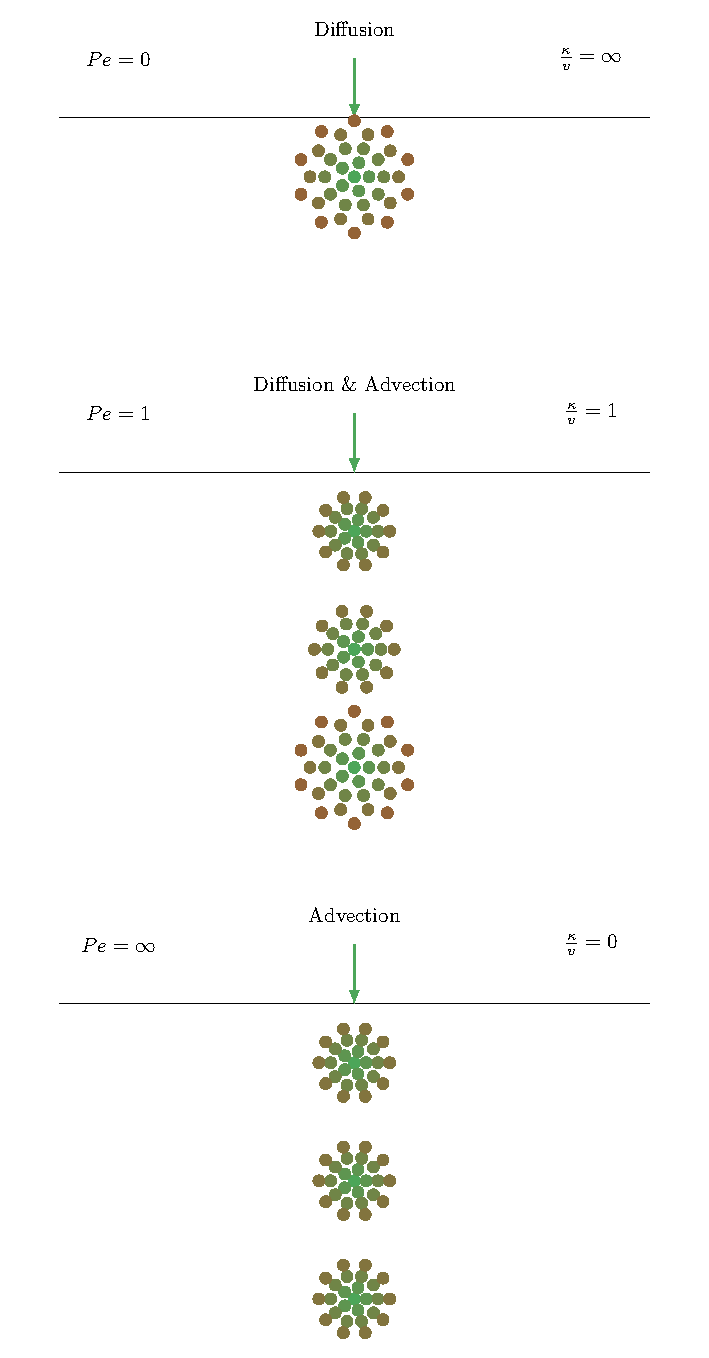
\includegraphics[scale=0.8]{Figures/AdvectionDiffusion.pdf} % requires the graphicx package
   \caption{Schematic representation of the role of the Péclet number, which is the inverse of the $\kappa/v$ ratio, on the type of vertical C transfer in a soil assuming a pulse of aboveground inputs. For a Péclet number of zero and $\kappa/v = \infty$, C entering the soil only moves due to diffusion (top); for a Péclet number and $\kappa/v = 1$, both diffusion and advection moves the carbon vertically (center); for a Péclet number of $\infty$ and $\kappa/v = 0$, C is only moved vertically by advective processes as in the case of DOC transport (bottom). }
   \label{fig:Peclet}
\end{figure}

In the analysis of partial differential equations, the Péclet number, defined as the ratio of advection to diffusion, plays a very important role in determining characteristics of the solution such as its numerical stability \citep{LeVeque2007}. In addition, the Péclet number can be used to determine the degree by which diffusion or advection may dominate the shape of a soil C profile (Figure \ref{fig:Peclet}). 

If soil C always decreases with depth \citep{Jobbagy2000}, the decomposition flux in equation \ref{eq:simpleCase} must be dominant across the entire soil profile so the rate of change with depth remains negative. In fact, this analysis suggests that the balance between lateral C inputs and decomposition is one of the main factors that affect the shape of soil C profiles where a continuous decrease in soil C is commonly observed. 

A corollary or implication provided by equation \ref{eq:simpleCase} is that if the decrease in soil C with depth follows a simple exponential function, the right hand side of equation \ref{eq:simpleCase} must be a constant value for all depths. This situation seems unlikely given the different interacting process that occur in a soil, and in fact, mathematical functions different than the simple exponential provide the best fit to observed data \citep{Jobbagy2000}.

\subsection{Numerical example} \label{sec:ex1}
We used equation \ref{eq:simpleCase} to investigate the role of diffusion, advection, decomposition and lateral inputs on the shape of idealized soil carbon profiles. 
We chose values of $\kappa$ and $v$ within the range of values obtained in previous models (Table \ref{tab:Models}) as well as representative functions for $k(d)$ and $u(d)$ within the range of previous studies \citep[e.g.][]{Elzein1995, Jackson1996, Jackson1997,Koven2013BGS}.

To investigate the effect of diffusion and advection, we ran simulations with values of $\kappa = \{0.1, 1, 5, 15\}$ cm$^2$ yr$^{-1}$ and $v = \{0.1, 1, 5, 10 \}$ cm yr$^{-1}$  (Figure \ref{fig:AdvectionDiffusion}), with root inputs and decomposition following equations \ref{eq:ud} and \ref{eq:kd} as described below. The results show that vertical transport processes tend to create a horizon with largest rate of change in concentrations of C with depth (1st derivative) close to the surface. This layer could be the result of either advection or diffusion (Figure \ref{fig:AdvectionDiffusion}). Because in these simulations, lateral root inputs and decomposition decrease with depth (see equations \ref{eq:ud}, and \ref{eq:kd} below), there is a general trend of C concentrations to decline to values close to zero. Therefore, vertical transport do not seem to play a major role in transporting carbon below 50 cm depth within the range of advection and diffusion values used in these simulations, which covers the entire range of values obtained in previous studies (Table \ref{tab:Models}). Only at high advection velocities ($v=10$ cm yr$^{-1}$) some carbon is transported below 50 cm depth, but this advection velocity is much higher than what has been used before in other models (Table \ref{tab:Models}).

\begin{figure}[htbp]
   \centering
   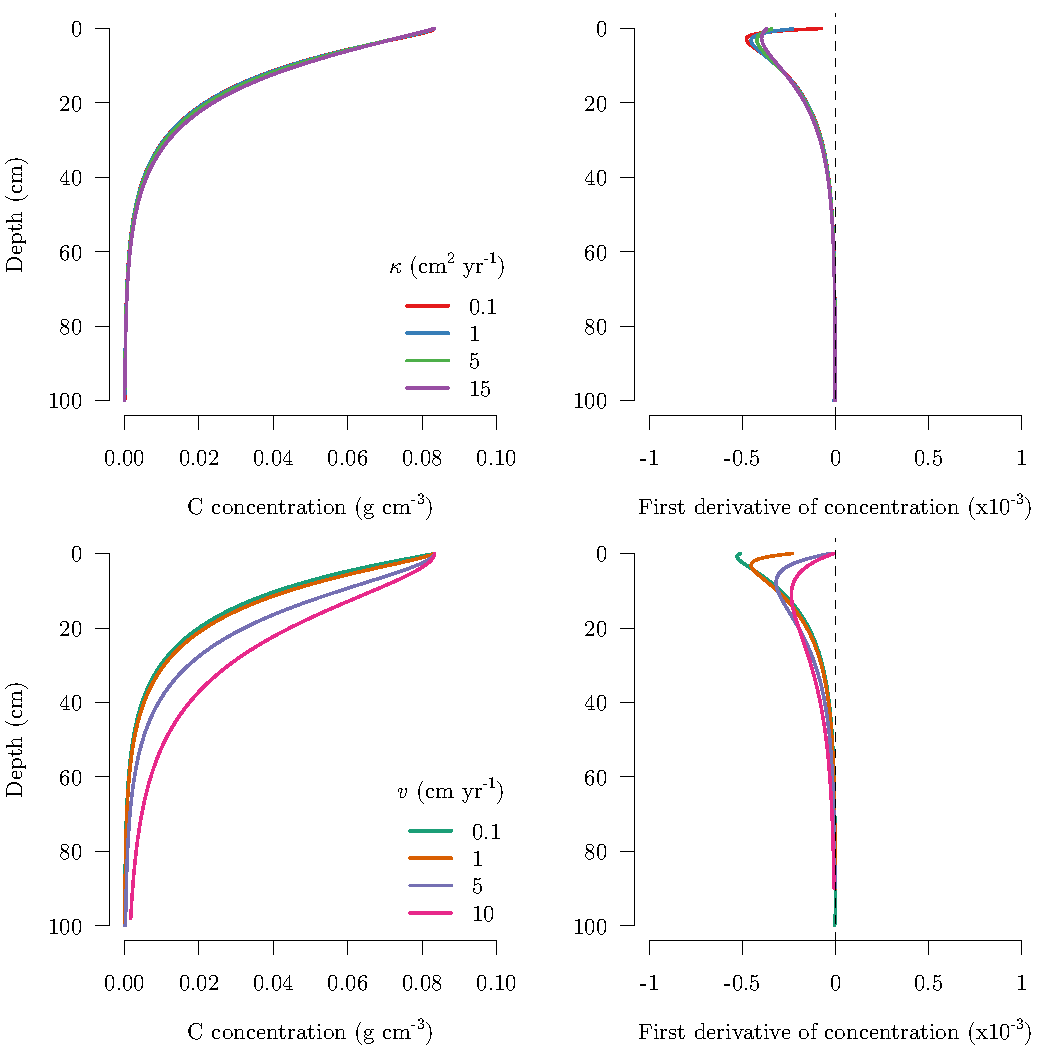
\includegraphics[width=\textwidth]{Figures/simulationsKappaV.pdf} % requires the graphicx package
   \caption{Numerical simulations of soil C depth profiles using the linear model with constant coefficients of equation \ref{eq:simpleCase}. The top panels show the C concentration and the first derivative of C concentrations for different values of $\kappa$ and a fixed value of $v = 1$ cm yr$^{-1}$. The bottom panels show C concentrations and their first derivative for different values of $v$ and a constant value of $\kappa = 1$ cm$^2$ yr$^{-1}$. }
   \label{fig:AdvectionDiffusion}
\end{figure}

The first derivative of the C concentration profiles with respect to depth from these simulations (Figure \ref{fig:AdvectionDiffusion} right panels), showed negative derivatives for the entire depth profile. According to equation \ref{eq:simpleCase}, the first derivative can only be positive if lateral root inputs and transport processes dominate over the decomposition flux, which is not the case in these simulations. The decomposition flux dominates over all other processes making the first derivative negative although approaching zero at deeper layers. As advection velocity increased, the first derivatives were less negative, indicating that as advective transport increases the change in C concentrations by depth is less pronounced.

In a second set of simulations, we practically removed advection and diffusion by making the value of these coefficients very small ($\kappa = v =0.01$) and represented lateral root inputs with the function

\begin{equation} \label{eq:ud}
u(d) = - \beta^d \ \ln \beta .
\end{equation}
This function predicts vertical root distributions and was originally proposed by \citet{Gale1987} and used by \citet{Jackson1996, Jackson1997} to obtain vertical root distributions at the biome level. The original function predicts the fraction of root biomass for each depth, and multiplied by an average root turnover rate of 1 yr$^{-1}$ \citep{Gill2000}, gives the proportion of root inputs per depth interval $u(d)$. For the simulations, we used values of $\beta : \{0.92, 0.95, 0.98 \}$ that include the observed extremes of values for shallow root systems ($\beta =0.92$) and deep root systems ($\beta = 0.98$) \citep{Gale1987, Jackson1996}.

The function used to represent decomposition rates by depth was extracted from \citet{Koven2013BGS}
\begin{equation} \label{eq:kd}
k(d) = k_0 \exp \left(\frac{-d}{d_e} \right),
\end{equation}
with the maximum decomposition rate at the surface given by $k_0 = k(d=0)$, and $d_e$ representing the e-folding depth of decomposition rates. In our simulations, we used values of $k_0 : \{1, 0.1, 0.01 \}$ yr$^{-1}$ and a constant value of $d_e = 90$ cm. Equation \ref{eq:kd} is an empirical function that accounts for unresolved processes such as changes in oxygen availability or microbial activity with depth, and therefore it could be considered as a place holder for other mechanistic representations of depth dependent microbial dynamics. 

The results from this second set of simulations evaluating the effect of lateral root inputs and decomposition showed that slowing down decomposition can have a significant effect on the shape of the vertical soil C profile (Figure \ref{fig:rootDecomp}). These results seem counterintuitive because equation \ref{eq:simpleCase} suggests that the negative term of the equation should be affected by larger values of $k(d)$, but because with slow decomposition higher amounts of C are obtained at steady-state, the entire term $k(d) x(d)$ is large, promoting a strong soil C gradient. The vertical distribution of root inputs has also a significant effect on the shape of the soil C profile, with shallow root inputs promoting a strong vertical gradient and deep rooting systems a more pronounced gradient with lower values of the first derivative (Figure \ref{fig:rootDecomp}). In this set of simulations, we observed also a maximum rate of change of C at the upper layers where the value of the first derivative reached a maximum. 

\begin{figure}[htbp]
   \centering
   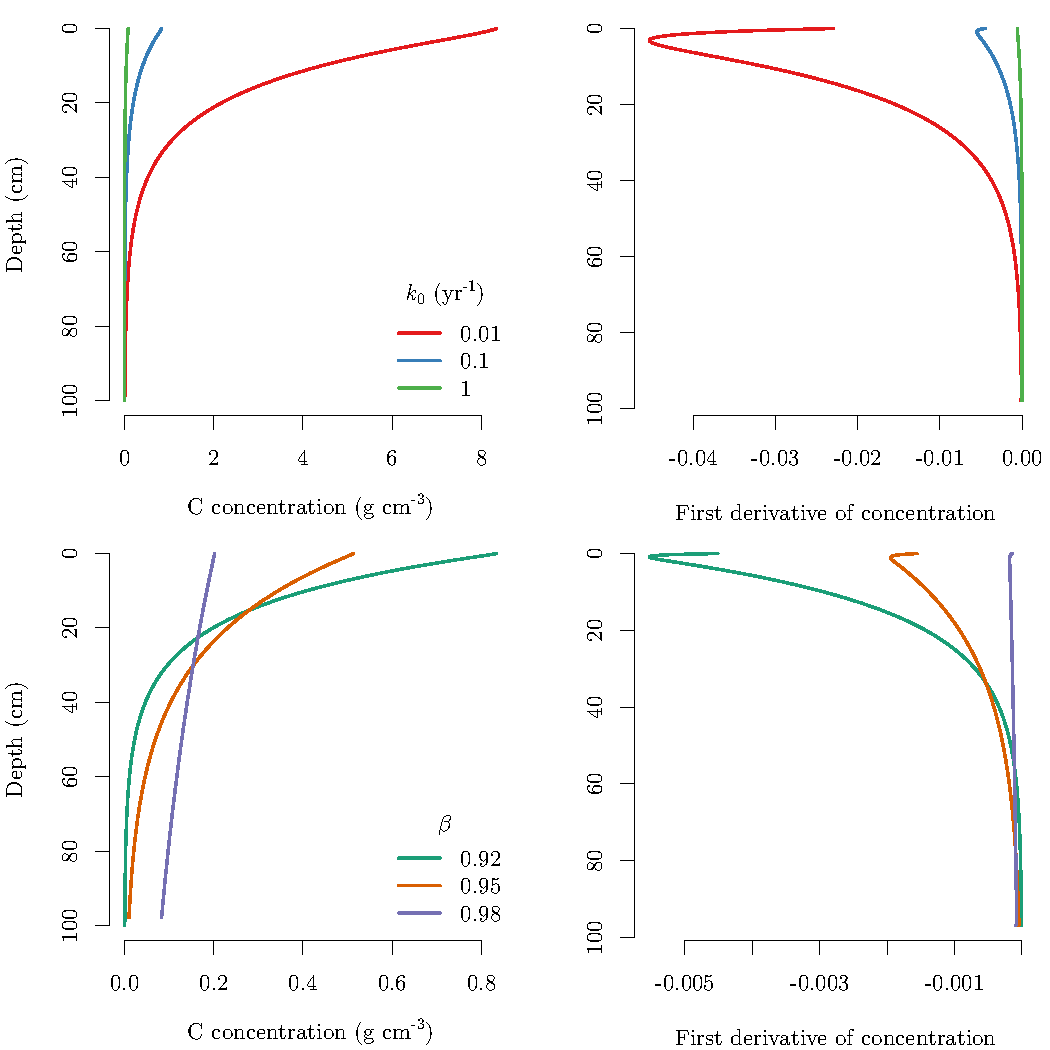
\includegraphics[width=\textwidth]{Figures/rootDecomp.pdf} % requires the graphicx package
%% Created by tikzDevice version 0.12.5 on 2023-12-13 16:26:35
% !TEX encoding = UTF-8 Unicode
\documentclass[10pt]{article}
\usepackage{tikz}

\usepackage[active,tightpage,psfixbb]{preview}

\PreviewEnvironment{pgfpicture}

\setlength\PreviewBorder{0pt}
\begin{document}

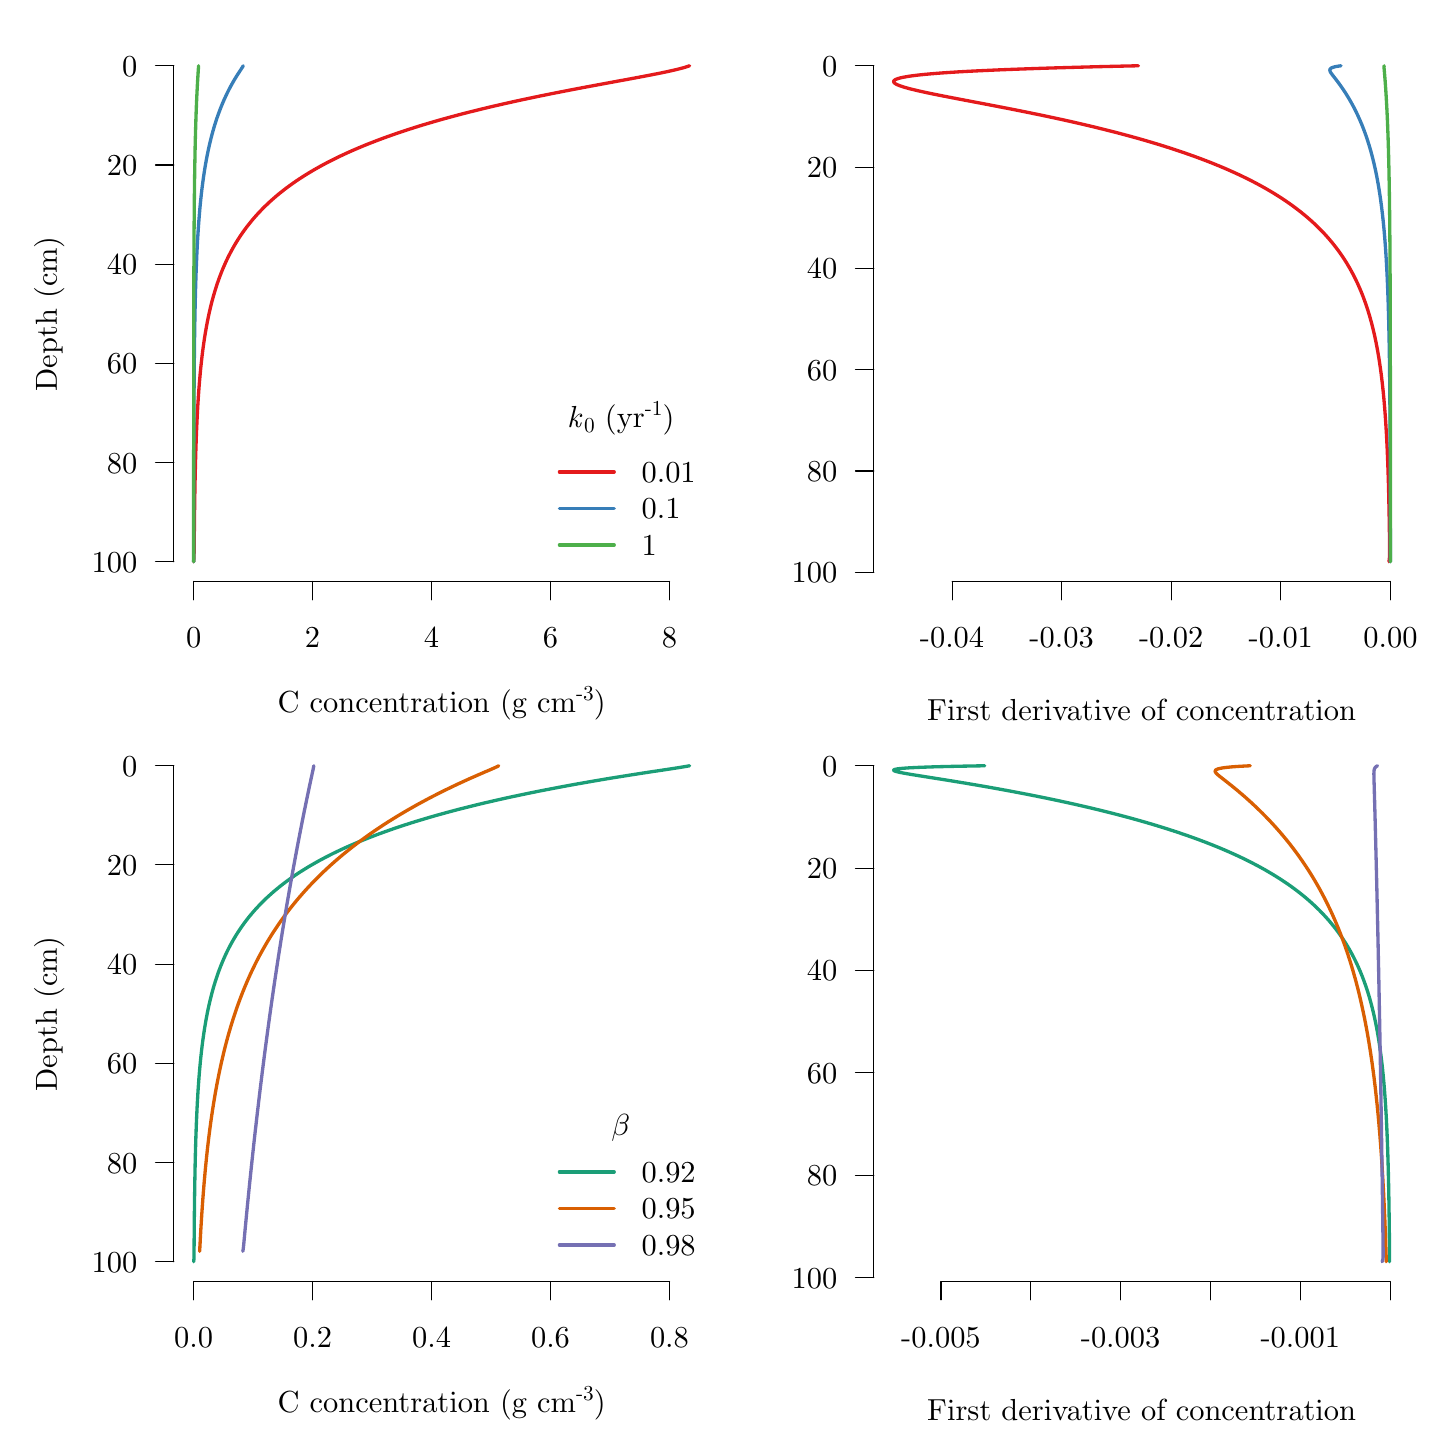
\begin{tikzpicture}[x=1pt,y=1pt]
\definecolor{fillColor}{RGB}{255,255,255}
\path[use as bounding box,fill=fillColor,fill opacity=0.00] (0,0) rectangle (505.89,505.89);
\begin{scope}
\path[clip] ( 52.80,305.75) rectangle (246.34,499.29);
\definecolor{drawColor}{RGB}{228,26,28}

\path[draw=drawColor,line width= 1.2pt,line join=round,line cap=round] (239.18,492.12) --
	(238.68,491.94) --
	(238.14,491.76) --
	(237.57,491.58) --
	(236.95,491.40) --
	(236.30,491.23) --
	(235.62,491.05) --
	(234.90,490.87) --
	(234.17,490.69) --
	(233.40,490.51) --
	(232.61,490.33) --
	(231.80,490.15) --
	(230.98,489.97) --
	(230.13,489.79) --
	(229.27,489.61) --
	(228.39,489.43) --
	(227.50,489.25) --
	(226.60,489.08) --
	(225.69,488.90) --
	(224.76,488.72) --
	(223.83,488.54) --
	(222.89,488.36) --
	(221.95,488.18) --
	(221.00,488.00) --
	(220.04,487.82) --
	(219.08,487.64) --
	(218.11,487.46) --
	(217.15,487.28) --
	(216.18,487.10) --
	(215.20,486.92) --
	(214.23,486.75) --
	(213.26,486.57) --
	(212.28,486.39) --
	(211.31,486.21) --
	(210.34,486.03) --
	(209.36,485.85) --
	(208.39,485.67) --
	(207.42,485.49) --
	(206.45,485.31) --
	(205.49,485.13) --
	(204.52,484.95) --
	(203.56,484.77) --
	(202.61,484.59) --
	(201.65,484.42) --
	(200.70,484.24) --
	(199.75,484.06) --
	(198.81,483.88) --
	(197.87,483.70) --
	(196.93,483.52) --
	(196.00,483.34) --
	(195.07,483.16) --
	(194.15,482.98) --
	(193.23,482.80) --
	(192.32,482.62) --
	(191.41,482.44) --
	(190.50,482.27) --
	(189.60,482.09) --
	(188.71,481.91) --
	(187.82,481.73) --
	(186.93,481.55) --
	(186.05,481.37) --
	(185.17,481.19) --
	(184.30,481.01) --
	(183.44,480.83) --
	(182.58,480.65) --
	(181.72,480.47) --
	(180.87,480.29) --
	(180.03,480.11) --
	(179.19,479.94) --
	(178.35,479.76) --
	(177.52,479.58) --
	(176.70,479.40) --
	(175.88,479.22) --
	(175.07,479.04) --
	(174.26,478.86) --
	(173.46,478.68) --
	(172.66,478.50) --
	(171.87,478.32) --
	(171.08,478.14) --
	(170.30,477.96) --
	(169.52,477.78) --
	(168.75,477.61) --
	(167.98,477.43) --
	(167.22,477.25) --
	(166.46,477.07) --
	(165.71,476.89) --
	(164.97,476.71) --
	(164.22,476.53) --
	(163.49,476.35) --
	(162.76,476.17) --
	(162.03,475.99) --
	(161.31,475.81) --
	(160.59,475.63) --
	(159.88,475.46) --
	(159.17,475.28) --
	(158.47,475.10) --
	(157.78,474.92) --
	(157.08,474.74) --
	(156.40,474.56) --
	(155.71,474.38) --
	(155.04,474.20) --
	(154.36,474.02) --
	(153.70,473.84) --
	(153.03,473.66) --
	(152.37,473.48) --
	(151.72,473.30) --
	(151.07,473.13) --
	(150.42,472.95) --
	(149.78,472.77) --
	(149.15,472.59) --
	(148.51,472.41) --
	(147.89,472.23) --
	(147.26,472.05) --
	(146.64,471.87) --
	(146.03,471.69) --
	(145.42,471.51) --
	(144.81,471.33) --
	(144.21,471.15) --
	(143.62,470.98) --
	(143.02,470.80) --
	(142.43,470.62) --
	(141.85,470.44) --
	(141.27,470.26) --
	(140.69,470.08) --
	(140.12,469.90) --
	(139.55,469.72) --
	(138.99,469.54) --
	(138.43,469.36) --
	(137.87,469.18) --
	(137.32,469.00) --
	(136.77,468.82) --
	(136.22,468.65) --
	(135.68,468.47) --
	(135.15,468.29) --
	(134.61,468.11) --
	(134.08,467.93) --
	(133.56,467.75) --
	(133.04,467.57) --
	(132.52,467.39) --
	(132.00,467.21) --
	(131.49,467.03) --
	(130.99,466.85) --
	(130.48,466.67) --
	(129.98,466.49) --
	(129.49,466.32) --
	(128.99,466.14) --
	(128.50,465.96) --
	(128.02,465.78) --
	(127.53,465.60) --
	(127.06,465.42) --
	(126.58,465.24) --
	(126.11,465.06) --
	(125.64,464.88) --
	(125.17,464.70) --
	(124.71,464.52) --
	(124.25,464.34) --
	(123.80,464.17) --
	(123.34,463.99) --
	(122.89,463.81) --
	(122.45,463.63) --
	(122.00,463.45) --
	(121.56,463.27) --
	(121.13,463.09) --
	(120.69,462.91) --
	(120.26,462.73) --
	(119.84,462.55) --
	(119.41,462.37) --
	(118.99,462.19) --
	(118.57,462.01) --
	(118.16,461.84) --
	(117.74,461.66) --
	(117.33,461.48) --
	(116.93,461.30) --
	(116.52,461.12) --
	(116.12,460.94) --
	(115.72,460.76) --
	(115.33,460.58) --
	(114.94,460.40) --
	(114.55,460.22) --
	(114.16,460.04) --
	(113.77,459.86) --
	(113.39,459.68) --
	(113.01,459.51) --
	(112.64,459.33) --
	(112.27,459.15) --
	(111.89,458.97) --
	(111.53,458.79) --
	(111.16,458.61) --
	(110.80,458.43) --
	(110.44,458.25) --
	(110.08,458.07) --
	(109.72,457.89) --
	(109.37,457.71) --
	(109.02,457.53) --
	(108.67,457.36) --
	(108.33,457.18) --
	(107.99,457.00) --
	(107.65,456.82) --
	(107.31,456.64) --
	(106.97,456.46) --
	(106.64,456.28) --
	(106.31,456.10) --
	(105.98,455.92) --
	(105.65,455.74) --
	(105.33,455.56) --
	(105.01,455.38) --
	(104.69,455.20) --
	(104.37,455.03) --
	(104.06,454.85) --
	(103.75,454.67) --
	(103.44,454.49) --
	(103.13,454.31) --
	(102.82,454.13) --
	(102.52,453.95) --
	(102.22,453.77) --
	(101.92,453.59) --
	(101.62,453.41) --
	(101.33,453.23) --
	(101.03,453.05) --
	(100.74,452.88) --
	(100.45,452.70) --
	(100.17,452.52) --
	( 99.88,452.34) --
	( 99.60,452.16) --
	( 99.32,451.98) --
	( 99.04,451.80) --
	( 98.76,451.62) --
	( 98.49,451.44) --
	( 98.21,451.26) --
	( 97.94,451.08) --
	( 97.67,450.90) --
	( 97.41,450.72) --
	( 97.14,450.55) --
	( 96.88,450.37) --
	( 96.62,450.19) --
	( 96.36,450.01) --
	( 96.10,449.83) --
	( 95.84,449.65) --
	( 95.59,449.47) --
	( 95.34,449.29) --
	( 95.09,449.11) --
	( 94.84,448.93) --
	( 94.59,448.75) --
	( 94.35,448.57) --
	( 94.10,448.39) --
	( 93.86,448.22) --
	( 93.62,448.04) --
	( 93.38,447.86) --
	( 93.15,447.68) --
	( 92.91,447.50) --
	( 92.68,447.32) --
	( 92.45,447.14) --
	( 92.22,446.96) --
	( 91.99,446.78) --
	( 91.76,446.60) --
	( 91.54,446.42) --
	( 91.31,446.24) --
	( 91.09,446.07) --
	( 90.87,445.89) --
	( 90.65,445.71) --
	( 90.44,445.53) --
	( 90.22,445.35) --
	( 90.01,445.17) --
	( 89.79,444.99) --
	( 89.58,444.81) --
	( 89.37,444.63) --
	( 89.16,444.45) --
	( 88.96,444.27) --
	( 88.75,444.09) --
	( 88.55,443.91) --
	( 88.35,443.74) --
	( 88.15,443.56) --
	( 87.95,443.38) --
	( 87.75,443.20) --
	( 87.55,443.02) --
	( 87.36,442.84) --
	( 87.16,442.66) --
	( 86.97,442.48) --
	( 86.78,442.30) --
	( 86.59,442.12) --
	( 86.40,441.94) --
	( 86.21,441.76) --
	( 86.03,441.58) --
	( 85.84,441.41) --
	( 85.66,441.23) --
	( 85.48,441.05) --
	( 85.30,440.87) --
	( 85.12,440.69) --
	( 84.94,440.51) --
	( 84.76,440.33) --
	( 84.59,440.15) --
	( 84.42,439.97) --
	( 84.24,439.79) --
	( 84.07,439.61) --
	( 83.90,439.43) --
	( 83.73,439.26) --
	( 83.56,439.08) --
	( 83.40,438.90) --
	( 83.23,438.72) --
	( 83.07,438.54) --
	( 82.90,438.36) --
	( 82.74,438.18) --
	( 82.58,438.00) --
	( 82.42,437.82) --
	( 82.26,437.64) --
	( 82.10,437.46) --
	( 81.95,437.28) --
	( 81.79,437.10) --
	( 81.64,436.93) --
	( 81.48,436.75) --
	( 81.33,436.57) --
	( 81.18,436.39) --
	( 81.03,436.21) --
	( 80.88,436.03) --
	( 80.73,435.85) --
	( 80.59,435.67) --
	( 80.44,435.49) --
	( 80.30,435.31) --
	( 80.15,435.13) --
	( 80.01,434.95) --
	( 79.87,434.77) --
	( 79.73,434.60) --
	( 79.59,434.42) --
	( 79.45,434.24) --
	( 79.31,434.06) --
	( 79.17,433.88) --
	( 79.04,433.70) --
	( 78.90,433.52) --
	( 78.77,433.34) --
	( 78.64,433.16) --
	( 78.50,432.98) --
	( 78.37,432.80) --
	( 78.24,432.62) --
	( 78.11,432.45) --
	( 77.99,432.27) --
	( 77.86,432.09) --
	( 77.73,431.91) --
	( 77.61,431.73) --
	( 77.48,431.55) --
	( 77.36,431.37) --
	( 77.24,431.19) --
	( 77.11,431.01) --
	( 76.99,430.83) --
	( 76.87,430.65) --
	( 76.75,430.47) --
	( 76.63,430.29) --
	( 76.52,430.12) --
	( 76.40,429.94) --
	( 76.28,429.76) --
	( 76.17,429.58) --
	( 76.05,429.40) --
	( 75.94,429.22) --
	( 75.83,429.04) --
	( 75.72,428.86) --
	( 75.60,428.68) --
	( 75.49,428.50) --
	( 75.38,428.32) --
	( 75.27,428.14) --
	( 75.17,427.97) --
	( 75.06,427.79) --
	( 74.95,427.61) --
	( 74.85,427.43) --
	( 74.74,427.25) --
	( 74.64,427.07) --
	( 74.53,426.89) --
	( 74.43,426.71) --
	( 74.33,426.53) --
	( 74.23,426.35) --
	( 74.13,426.17) --
	( 74.03,425.99) --
	( 73.93,425.81) --
	( 73.83,425.64) --
	( 73.73,425.46) --
	( 73.63,425.28) --
	( 73.54,425.10) --
	( 73.44,424.92) --
	( 73.35,424.74) --
	( 73.25,424.56) --
	( 73.16,424.38) --
	( 73.07,424.20) --
	( 72.97,424.02) --
	( 72.88,423.84) --
	( 72.79,423.66) --
	( 72.70,423.48) --
	( 72.61,423.31) --
	( 72.52,423.13) --
	( 72.43,422.95) --
	( 72.34,422.77) --
	( 72.26,422.59) --
	( 72.17,422.41) --
	( 72.08,422.23) --
	( 72.00,422.05) --
	( 71.91,421.87) --
	( 71.83,421.69) --
	( 71.74,421.51) --
	( 71.66,421.33) --
	( 71.58,421.16) --
	( 71.50,420.98) --
	( 71.42,420.80) --
	( 71.34,420.62) --
	( 71.26,420.44) --
	( 71.18,420.26) --
	( 71.10,420.08) --
	( 71.02,419.90) --
	( 70.94,419.72) --
	( 70.86,419.54) --
	( 70.79,419.36) --
	( 70.71,419.18) --
	( 70.63,419.00) --
	( 70.56,418.83) --
	( 70.48,418.65) --
	( 70.41,418.47) --
	( 70.34,418.29) --
	( 70.26,418.11) --
	( 70.19,417.93) --
	( 70.12,417.75) --
	( 70.05,417.57) --
	( 69.98,417.39) --
	( 69.90,417.21) --
	( 69.83,417.03) --
	( 69.76,416.85) --
	( 69.70,416.67) --
	( 69.63,416.50) --
	( 69.56,416.32) --
	( 69.49,416.14) --
	( 69.42,415.96) --
	( 69.36,415.78) --
	( 69.29,415.60) --
	( 69.23,415.42) --
	( 69.16,415.24) --
	( 69.10,415.06) --
	( 69.03,414.88) --
	( 68.97,414.70) --
	( 68.90,414.52) --
	( 68.84,414.35) --
	( 68.78,414.17) --
	( 68.72,413.99) --
	( 68.65,413.81) --
	( 68.59,413.63) --
	( 68.53,413.45) --
	( 68.47,413.27) --
	( 68.41,413.09) --
	( 68.35,412.91) --
	( 68.29,412.73) --
	( 68.23,412.55) --
	( 68.18,412.37) --
	( 68.12,412.19) --
	( 68.06,412.02) --
	( 68.00,411.84) --
	( 67.95,411.66) --
	( 67.89,411.48) --
	( 67.84,411.30) --
	( 67.78,411.12) --
	( 67.73,410.94) --
	( 67.67,410.76) --
	( 67.62,410.58) --
	( 67.56,410.40) --
	( 67.51,410.22) --
	( 67.46,410.04) --
	( 67.40,409.87) --
	( 67.35,409.69) --
	( 67.30,409.51) --
	( 67.25,409.33) --
	( 67.20,409.15) --
	( 67.14,408.97) --
	( 67.09,408.79) --
	( 67.04,408.61) --
	( 66.99,408.43) --
	( 66.94,408.25) --
	( 66.90,408.07) --
	( 66.85,407.89) --
	( 66.80,407.71) --
	( 66.75,407.54) --
	( 66.70,407.36) --
	( 66.65,407.18) --
	( 66.61,407.00) --
	( 66.56,406.82) --
	( 66.51,406.64) --
	( 66.47,406.46) --
	( 66.42,406.28) --
	( 66.38,406.10) --
	( 66.33,405.92) --
	( 66.29,405.74) --
	( 66.24,405.56) --
	( 66.20,405.38) --
	( 66.15,405.21) --
	( 66.11,405.03) --
	( 66.07,404.85) --
	( 66.02,404.67) --
	( 65.98,404.49) --
	( 65.94,404.31) --
	( 65.90,404.13) --
	( 65.86,403.95) --
	( 65.81,403.77) --
	( 65.77,403.59) --
	( 65.73,403.41) --
	( 65.69,403.23) --
	( 65.65,403.06) --
	( 65.61,402.88) --
	( 65.57,402.70) --
	( 65.53,402.52) --
	( 65.49,402.34) --
	( 65.45,402.16) --
	( 65.42,401.98) --
	( 65.38,401.80) --
	( 65.34,401.62) --
	( 65.30,401.44) --
	( 65.26,401.26) --
	( 65.23,401.08) --
	( 65.19,400.90) --
	( 65.15,400.73) --
	( 65.12,400.55) --
	( 65.08,400.37) --
	( 65.04,400.19) --
	( 65.01,400.01) --
	( 64.97,399.83) --
	( 64.94,399.65) --
	( 64.90,399.47) --
	( 64.87,399.29) --
	( 64.83,399.11) --
	( 64.80,398.93) --
	( 64.77,398.75) --
	( 64.73,398.57) --
	( 64.70,398.40) --
	( 64.67,398.22) --
	( 64.63,398.04) --
	( 64.60,397.86) --
	( 64.57,397.68) --
	( 64.53,397.50) --
	( 64.50,397.32) --
	( 64.47,397.14) --
	( 64.44,396.96) --
	( 64.41,396.78) --
	( 64.38,396.60) --
	( 64.35,396.42) --
	( 64.31,396.25) --
	( 64.28,396.07) --
	( 64.25,395.89) --
	( 64.22,395.71) --
	( 64.19,395.53) --
	( 64.16,395.35) --
	( 64.13,395.17) --
	( 64.11,394.99) --
	( 64.08,394.81) --
	( 64.05,394.63) --
	( 64.02,394.45) --
	( 63.99,394.27) --
	( 63.96,394.09) --
	( 63.93,393.92) --
	( 63.91,393.74) --
	( 63.88,393.56) --
	( 63.85,393.38) --
	( 63.82,393.20) --
	( 63.80,393.02) --
	( 63.77,392.84) --
	( 63.74,392.66) --
	( 63.72,392.48) --
	( 63.69,392.30) --
	( 63.66,392.12) --
	( 63.64,391.94) --
	( 63.61,391.76) --
	( 63.59,391.59) --
	( 63.56,391.41) --
	( 63.54,391.23) --
	( 63.51,391.05) --
	( 63.49,390.87) --
	( 63.46,390.69) --
	( 63.44,390.51) --
	( 63.41,390.33) --
	( 63.39,390.15) --
	( 63.36,389.97) --
	( 63.34,389.79) --
	( 63.32,389.61) --
	( 63.29,389.44) --
	( 63.27,389.26) --
	( 63.25,389.08) --
	( 63.22,388.90) --
	( 63.20,388.72) --
	( 63.18,388.54) --
	( 63.16,388.36) --
	( 63.13,388.18) --
	( 63.11,388.00) --
	( 63.09,387.82) --
	( 63.07,387.64) --
	( 63.04,387.46) --
	( 63.02,387.28) --
	( 63.00,387.11) --
	( 62.98,386.93) --
	( 62.96,386.75) --
	( 62.94,386.57) --
	( 62.92,386.39) --
	( 62.90,386.21) --
	( 62.88,386.03) --
	( 62.86,385.85) --
	( 62.84,385.67) --
	( 62.82,385.49) --
	( 62.80,385.31) --
	( 62.78,385.13) --
	( 62.76,384.96) --
	( 62.74,384.78) --
	( 62.72,384.60) --
	( 62.70,384.42) --
	( 62.68,384.24) --
	( 62.66,384.06) --
	( 62.64,383.88) --
	( 62.62,383.70) --
	( 62.60,383.52) --
	( 62.58,383.34) --
	( 62.57,383.16) --
	( 62.55,382.98) --
	( 62.53,382.80) --
	( 62.51,382.63) --
	( 62.49,382.45) --
	( 62.48,382.27) --
	( 62.46,382.09) --
	( 62.44,381.91) --
	( 62.42,381.73) --
	( 62.41,381.55) --
	( 62.39,381.37) --
	( 62.37,381.19) --
	( 62.36,381.01) --
	( 62.34,380.83) --
	( 62.32,380.65) --
	( 62.31,380.47) --
	( 62.29,380.30) --
	( 62.27,380.12) --
	( 62.26,379.94) --
	( 62.24,379.76) --
	( 62.23,379.58) --
	( 62.21,379.40) --
	( 62.19,379.22) --
	( 62.18,379.04) --
	( 62.16,378.86) --
	( 62.15,378.68) --
	( 62.13,378.50) --
	( 62.12,378.32) --
	( 62.10,378.15) --
	( 62.09,377.97) --
	( 62.07,377.79) --
	( 62.06,377.61) --
	( 62.04,377.43) --
	( 62.03,377.25) --
	( 62.01,377.07) --
	( 62.00,376.89) --
	( 61.99,376.71) --
	( 61.97,376.53) --
	( 61.96,376.35) --
	( 61.94,376.17) --
	( 61.93,375.99) --
	( 61.92,375.82) --
	( 61.90,375.64) --
	( 61.89,375.46) --
	( 61.87,375.28) --
	( 61.86,375.10) --
	( 61.85,374.92) --
	( 61.84,374.74) --
	( 61.82,374.56) --
	( 61.81,374.38) --
	( 61.80,374.20) --
	( 61.78,374.02) --
	( 61.77,373.84) --
	( 61.76,373.66) --
	( 61.75,373.49) --
	( 61.73,373.31) --
	( 61.72,373.13) --
	( 61.71,372.95) --
	( 61.70,372.77) --
	( 61.68,372.59) --
	( 61.67,372.41) --
	( 61.66,372.23) --
	( 61.65,372.05) --
	( 61.64,371.87) --
	( 61.62,371.69) --
	( 61.61,371.51) --
	( 61.60,371.34) --
	( 61.59,371.16) --
	( 61.58,370.98) --
	( 61.57,370.80) --
	( 61.56,370.62) --
	( 61.55,370.44) --
	( 61.53,370.26) --
	( 61.52,370.08) --
	( 61.51,369.90) --
	( 61.50,369.72) --
	( 61.49,369.54) --
	( 61.48,369.36) --
	( 61.47,369.18) --
	( 61.46,369.01) --
	( 61.45,368.83) --
	( 61.44,368.65) --
	( 61.43,368.47) --
	( 61.42,368.29) --
	( 61.41,368.11) --
	( 61.40,367.93) --
	( 61.39,367.75) --
	( 61.38,367.57) --
	( 61.37,367.39) --
	( 61.36,367.21) --
	( 61.35,367.03) --
	( 61.34,366.86) --
	( 61.33,366.68) --
	( 61.32,366.50) --
	( 61.31,366.32) --
	( 61.30,366.14) --
	( 61.29,365.96) --
	( 61.28,365.78) --
	( 61.27,365.60) --
	( 61.26,365.42) --
	( 61.25,365.24) --
	( 61.25,365.06) --
	( 61.24,364.88) --
	( 61.23,364.70) --
	( 61.22,364.53) --
	( 61.21,364.35) --
	( 61.20,364.17) --
	( 61.19,363.99) --
	( 61.18,363.81) --
	( 61.18,363.63) --
	( 61.17,363.45) --
	( 61.16,363.27) --
	( 61.15,363.09) --
	( 61.14,362.91) --
	( 61.13,362.73) --
	( 61.13,362.55) --
	( 61.12,362.37) --
	( 61.11,362.20) --
	( 61.10,362.02) --
	( 61.09,361.84) --
	( 61.09,361.66) --
	( 61.08,361.48) --
	( 61.07,361.30) --
	( 61.06,361.12) --
	( 61.06,360.94) --
	( 61.05,360.76) --
	( 61.04,360.58) --
	( 61.03,360.40) --
	( 61.03,360.22) --
	( 61.02,360.05) --
	( 61.01,359.87) --
	( 61.00,359.69) --
	( 61.00,359.51) --
	( 60.99,359.33) --
	( 60.98,359.15) --
	( 60.98,358.97) --
	( 60.97,358.79) --
	( 60.96,358.61) --
	( 60.95,358.43) --
	( 60.95,358.25) --
	( 60.94,358.07) --
	( 60.93,357.89) --
	( 60.93,357.72) --
	( 60.92,357.54) --
	( 60.91,357.36) --
	( 60.91,357.18) --
	( 60.90,357.00) --
	( 60.89,356.82) --
	( 60.89,356.64) --
	( 60.88,356.46) --
	( 60.87,356.28) --
	( 60.87,356.10) --
	( 60.86,355.92) --
	( 60.86,355.74) --
	( 60.85,355.56) --
	( 60.84,355.39) --
	( 60.84,355.21) --
	( 60.83,355.03) --
	( 60.83,354.85) --
	( 60.82,354.67) --
	( 60.81,354.49) --
	( 60.81,354.31) --
	( 60.80,354.13) --
	( 60.80,353.95) --
	( 60.79,353.77) --
	( 60.78,353.59) --
	( 60.78,353.41) --
	( 60.77,353.24) --
	( 60.77,353.06) --
	( 60.76,352.88) --
	( 60.76,352.70) --
	( 60.75,352.52) --
	( 60.75,352.34) --
	( 60.74,352.16) --
	( 60.73,351.98) --
	( 60.73,351.80) --
	( 60.72,351.62) --
	( 60.72,351.44) --
	( 60.71,351.26) --
	( 60.71,351.08) --
	( 60.70,350.91) --
	( 60.70,350.73) --
	( 60.69,350.55) --
	( 60.69,350.37) --
	( 60.68,350.19) --
	( 60.68,350.01) --
	( 60.67,349.83) --
	( 60.67,349.65) --
	( 60.66,349.47) --
	( 60.66,349.29) --
	( 60.65,349.11) --
	( 60.65,348.93) --
	( 60.64,348.75) --
	( 60.64,348.58) --
	( 60.63,348.40) --
	( 60.63,348.22) --
	( 60.63,348.04) --
	( 60.62,347.86) --
	( 60.62,347.68) --
	( 60.61,347.50) --
	( 60.61,347.32) --
	( 60.60,347.14) --
	( 60.60,346.96) --
	( 60.59,346.78) --
	( 60.59,346.60) --
	( 60.59,346.43) --
	( 60.58,346.25) --
	( 60.58,346.07) --
	( 60.57,345.89) --
	( 60.57,345.71) --
	( 60.56,345.53) --
	( 60.56,345.35) --
	( 60.56,345.17) --
	( 60.55,344.99) --
	( 60.55,344.81) --
	( 60.54,344.63) --
	( 60.54,344.45) --
	( 60.54,344.27) --
	( 60.53,344.10) --
	( 60.53,343.92) --
	( 60.52,343.74) --
	( 60.52,343.56) --
	( 60.52,343.38) --
	( 60.51,343.20) --
	( 60.51,343.02) --
	( 60.50,342.84) --
	( 60.50,342.66) --
	( 60.50,342.48) --
	( 60.49,342.30) --
	( 60.49,342.12) --
	( 60.49,341.95) --
	( 60.48,341.77) --
	( 60.48,341.59) --
	( 60.48,341.41) --
	( 60.47,341.23) --
	( 60.47,341.05) --
	( 60.47,340.87) --
	( 60.46,340.69) --
	( 60.46,340.51) --
	( 60.45,340.33) --
	( 60.45,340.15) --
	( 60.45,339.97) --
	( 60.44,339.79) --
	( 60.44,339.62) --
	( 60.44,339.44) --
	( 60.43,339.26) --
	( 60.43,339.08) --
	( 60.43,338.90) --
	( 60.43,338.72) --
	( 60.42,338.54) --
	( 60.42,338.36) --
	( 60.42,338.18) --
	( 60.41,338.00) --
	( 60.41,337.82) --
	( 60.41,337.64) --
	( 60.40,337.46) --
	( 60.40,337.29) --
	( 60.40,337.11) --
	( 60.39,336.93) --
	( 60.39,336.75) --
	( 60.39,336.57) --
	( 60.39,336.39) --
	( 60.38,336.21) --
	( 60.38,336.03) --
	( 60.38,335.85) --
	( 60.37,335.67) --
	( 60.37,335.49) --
	( 60.37,335.31) --
	( 60.37,335.14) --
	( 60.36,334.96) --
	( 60.36,334.78) --
	( 60.36,334.60) --
	( 60.35,334.42) --
	( 60.35,334.24) --
	( 60.35,334.06) --
	( 60.35,333.88) --
	( 60.34,333.70) --
	( 60.34,333.52) --
	( 60.34,333.34) --
	( 60.34,333.16) --
	( 60.33,332.98) --
	( 60.33,332.81) --
	( 60.33,332.63) --
	( 60.33,332.45) --
	( 60.32,332.27) --
	( 60.32,332.09) --
	( 60.32,331.91) --
	( 60.32,331.73) --
	( 60.31,331.55) --
	( 60.31,331.37) --
	( 60.31,331.19) --
	( 60.31,331.01) --
	( 60.30,330.83) --
	( 60.30,330.65) --
	( 60.30,330.48) --
	( 60.30,330.30) --
	( 60.30,330.12) --
	( 60.29,329.94) --
	( 60.29,329.76) --
	( 60.29,329.58) --
	( 60.29,329.40) --
	( 60.28,329.22) --
	( 60.28,329.04) --
	( 60.28,328.86) --
	( 60.28,328.68) --
	( 60.28,328.50) --
	( 60.27,328.33) --
	( 60.27,328.15) --
	( 60.27,327.97) --
	( 60.27,327.79) --
	( 60.27,327.61) --
	( 60.26,327.43) --
	( 60.26,327.25) --
	( 60.26,327.07) --
	( 60.26,326.89) --
	( 60.25,326.71) --
	( 60.25,326.53) --
	( 60.25,326.35) --
	( 60.25,326.17) --
	( 60.25,326.00) --
	( 60.25,325.82) --
	( 60.24,325.64) --
	( 60.24,325.46) --
	( 60.24,325.28) --
	( 60.24,325.10) --
	( 60.24,324.92) --
	( 60.23,324.74) --
	( 60.23,324.56) --
	( 60.23,324.38) --
	( 60.23,324.20) --
	( 60.23,324.02) --
	( 60.22,323.85) --
	( 60.22,323.67) --
	( 60.22,323.49) --
	( 60.22,323.31) --
	( 60.22,323.13) --
	( 60.22,322.95) --
	( 60.21,322.77) --
	( 60.21,322.59) --
	( 60.21,322.41) --
	( 60.21,322.23) --
	( 60.21,322.05) --
	( 60.21,321.87) --
	( 60.20,321.69) --
	( 60.20,321.52) --
	( 60.20,321.34) --
	( 60.20,321.16) --
	( 60.20,320.98) --
	( 60.20,320.80) --
	( 60.19,320.62) --
	( 60.19,320.44) --
	( 60.19,320.26) --
	( 60.19,320.08) --
	( 60.19,319.90) --
	( 60.19,319.72) --
	( 60.18,319.54) --
	( 60.18,319.36) --
	( 60.18,319.19) --
	( 60.18,319.01) --
	( 60.18,318.83) --
	( 60.18,318.65) --
	( 60.17,318.47) --
	( 60.17,318.29) --
	( 60.17,318.11) --
	( 60.17,317.93) --
	( 60.17,317.75) --
	( 60.16,317.57) --
	( 60.16,317.39) --
	( 60.16,317.21) --
	( 60.16,317.04) --
	( 60.15,316.86) --
	( 60.15,316.68) --
	( 60.15,316.50) --
	( 60.14,316.32) --
	( 60.14,316.14) --
	( 60.14,315.96) --
	( 60.13,315.78) --
	( 60.13,315.60) --
	( 60.12,315.42) --
	( 60.12,315.24) --
	( 60.11,315.06) --
	( 60.11,314.88) --
	( 60.10,314.71) --
	( 60.09,314.53) --
	( 60.08,314.35) --
	( 60.08,314.17) --
	( 60.06,313.99) --
	( 60.05,313.81) --
	( 60.04,313.63) --
	( 60.02,313.45) --
	( 60.01,313.27) --
	( 59.99,313.09) --
	( 59.97,312.91);
\end{scope}
\begin{scope}
\path[clip] (  0.00,  0.00) rectangle (505.89,505.89);
\definecolor{drawColor}{RGB}{0,0,0}

\path[draw=drawColor,line width= 0.4pt,line join=round,line cap=round] ( 59.97,305.75) -- (231.91,305.75);

\path[draw=drawColor,line width= 0.4pt,line join=round,line cap=round] ( 59.97,305.75) -- ( 59.97,299.14);

\path[draw=drawColor,line width= 0.4pt,line join=round,line cap=round] (102.95,305.75) -- (102.95,299.14);

\path[draw=drawColor,line width= 0.4pt,line join=round,line cap=round] (145.94,305.75) -- (145.94,299.14);

\path[draw=drawColor,line width= 0.4pt,line join=round,line cap=round] (188.92,305.75) -- (188.92,299.14);

\path[draw=drawColor,line width= 0.4pt,line join=round,line cap=round] (231.91,305.75) -- (231.91,299.14);

\node[text=drawColor,anchor=base,inner sep=0pt, outer sep=0pt, scale=  1.10] at ( 59.97,281.99) {0};

\node[text=drawColor,anchor=base,inner sep=0pt, outer sep=0pt, scale=  1.10] at (102.95,281.99) {2};

\node[text=drawColor,anchor=base,inner sep=0pt, outer sep=0pt, scale=  1.10] at (145.94,281.99) {4};

\node[text=drawColor,anchor=base,inner sep=0pt, outer sep=0pt, scale=  1.10] at (188.92,281.99) {6};

\node[text=drawColor,anchor=base,inner sep=0pt, outer sep=0pt, scale=  1.10] at (231.91,281.99) {8};
\end{scope}
\begin{scope}
\path[clip] (  0.00,252.94) rectangle (252.94,505.89);
\definecolor{drawColor}{RGB}{0,0,0}

\node[text=drawColor,anchor=base west,inner sep=0pt, outer sep=0pt, scale=  1.10] at ( 90.29,258.33) {C concentration (g c};

\node[text=drawColor,anchor=base west,inner sep=0pt, outer sep=0pt, scale=  1.10] at (189.00,258.33) {m};

\node[text=drawColor,anchor=base west,inner sep=0pt, outer sep=0pt, scale=  0.77] at (198.16,262.83) {-};

\node[text=drawColor,anchor=base west,inner sep=0pt, outer sep=0pt, scale=  0.77] at (200.73,262.83) {3};

\node[text=drawColor,anchor=base west,inner sep=0pt, outer sep=0pt, scale=  1.10] at (204.57,258.33) {)};

\node[text=drawColor,rotate= 90.00,anchor=base,inner sep=0pt, outer sep=0pt, scale=  1.10] at ( 10.56,402.52) {Depth (cm)};
\end{scope}
\begin{scope}
\path[clip] (  0.00,  0.00) rectangle (505.89,505.89);
\definecolor{drawColor}{RGB}{0,0,0}

\path[draw=drawColor,line width= 0.4pt,line join=round,line cap=round] ( 52.80,312.91) -- ( 52.80,492.12);

\path[draw=drawColor,line width= 0.4pt,line join=round,line cap=round] ( 52.80,312.91) -- ( 46.20,312.91);

\path[draw=drawColor,line width= 0.4pt,line join=round,line cap=round] ( 52.80,348.75) -- ( 46.20,348.75);

\path[draw=drawColor,line width= 0.4pt,line join=round,line cap=round] ( 52.80,384.60) -- ( 46.20,384.60);

\path[draw=drawColor,line width= 0.4pt,line join=round,line cap=round] ( 52.80,420.44) -- ( 46.20,420.44);

\path[draw=drawColor,line width= 0.4pt,line join=round,line cap=round] ( 52.80,456.28) -- ( 46.20,456.28);

\path[draw=drawColor,line width= 0.4pt,line join=round,line cap=round] ( 52.80,492.12) -- ( 46.20,492.12);

\node[text=drawColor,anchor=base east,inner sep=0pt, outer sep=0pt, scale=  1.10] at ( 39.60,309.13) {100};

\node[text=drawColor,anchor=base east,inner sep=0pt, outer sep=0pt, scale=  1.10] at ( 39.60,344.97) {80};

\node[text=drawColor,anchor=base east,inner sep=0pt, outer sep=0pt, scale=  1.10] at ( 39.60,380.81) {60};

\node[text=drawColor,anchor=base east,inner sep=0pt, outer sep=0pt, scale=  1.10] at ( 39.60,416.65) {40};

\node[text=drawColor,anchor=base east,inner sep=0pt, outer sep=0pt, scale=  1.10] at ( 39.60,452.49) {20};

\node[text=drawColor,anchor=base east,inner sep=0pt, outer sep=0pt, scale=  1.10] at ( 39.60,488.33) {0};
\end{scope}
\begin{scope}
\path[clip] ( 52.80,305.75) rectangle (246.34,499.29);
\definecolor{drawColor}{RGB}{55,126,184}

\path[draw=drawColor,line width= 1.2pt,line join=round,line cap=round] ( 77.89,492.12) --
	( 77.79,491.94) --
	( 77.69,491.76) --
	( 77.58,491.58) --
	( 77.47,491.40) --
	( 77.35,491.23) --
	( 77.24,491.05) --
	( 77.12,490.87) --
	( 77.00,490.69) --
	( 76.88,490.51) --
	( 76.76,490.33) --
	( 76.64,490.15) --
	( 76.52,489.97) --
	( 76.41,489.79) --
	( 76.29,489.61) --
	( 76.17,489.43) --
	( 76.06,489.25) --
	( 75.94,489.08) --
	( 75.83,488.90) --
	( 75.71,488.72) --
	( 75.60,488.54) --
	( 75.49,488.36) --
	( 75.38,488.18) --
	( 75.27,488.00) --
	( 75.16,487.82) --
	( 75.05,487.64) --
	( 74.94,487.46) --
	( 74.83,487.28) --
	( 74.72,487.10) --
	( 74.62,486.92) --
	( 74.51,486.75) --
	( 74.41,486.57) --
	( 74.30,486.39) --
	( 74.20,486.21) --
	( 74.10,486.03) --
	( 74.00,485.85) --
	( 73.90,485.67) --
	( 73.80,485.49) --
	( 73.70,485.31) --
	( 73.60,485.13) --
	( 73.50,484.95) --
	( 73.40,484.77) --
	( 73.31,484.59) --
	( 73.21,484.42) --
	( 73.11,484.24) --
	( 73.02,484.06) --
	( 72.93,483.88) --
	( 72.83,483.70) --
	( 72.74,483.52) --
	( 72.65,483.34) --
	( 72.56,483.16) --
	( 72.47,482.98) --
	( 72.38,482.80) --
	( 72.29,482.62) --
	( 72.20,482.44) --
	( 72.11,482.27) --
	( 72.02,482.09) --
	( 71.94,481.91) --
	( 71.85,481.73) --
	( 71.77,481.55) --
	( 71.68,481.37) --
	( 71.60,481.19) --
	( 71.51,481.01) --
	( 71.43,480.83) --
	( 71.35,480.65) --
	( 71.27,480.47) --
	( 71.18,480.29) --
	( 71.10,480.11) --
	( 71.02,479.94) --
	( 70.94,479.76) --
	( 70.87,479.58) --
	( 70.79,479.40) --
	( 70.71,479.22) --
	( 70.63,479.04) --
	( 70.56,478.86) --
	( 70.48,478.68) --
	( 70.40,478.50) --
	( 70.33,478.32) --
	( 70.25,478.14) --
	( 70.18,477.96) --
	( 70.11,477.78) --
	( 70.03,477.61) --
	( 69.96,477.43) --
	( 69.89,477.25) --
	( 69.82,477.07) --
	( 69.75,476.89) --
	( 69.68,476.71) --
	( 69.61,476.53) --
	( 69.54,476.35) --
	( 69.47,476.17) --
	( 69.40,475.99) --
	( 69.33,475.81) --
	( 69.27,475.63) --
	( 69.20,475.46) --
	( 69.13,475.28) --
	( 69.07,475.10) --
	( 69.00,474.92) --
	( 68.94,474.74) --
	( 68.87,474.56) --
	( 68.81,474.38) --
	( 68.74,474.20) --
	( 68.68,474.02) --
	( 68.62,473.84) --
	( 68.56,473.66) --
	( 68.49,473.48) --
	( 68.43,473.30) --
	( 68.37,473.13) --
	( 68.31,472.95) --
	( 68.25,472.77) --
	( 68.19,472.59) --
	( 68.13,472.41) --
	( 68.07,472.23) --
	( 68.02,472.05) --
	( 67.96,471.87) --
	( 67.90,471.69) --
	( 67.84,471.51) --
	( 67.79,471.33) --
	( 67.73,471.15) --
	( 67.67,470.98) --
	( 67.62,470.80) --
	( 67.56,470.62) --
	( 67.51,470.44) --
	( 67.46,470.26) --
	( 67.40,470.08) --
	( 67.35,469.90) --
	( 67.29,469.72) --
	( 67.24,469.54) --
	( 67.19,469.36) --
	( 67.14,469.18) --
	( 67.09,469.00) --
	( 67.04,468.82) --
	( 66.98,468.65) --
	( 66.93,468.47) --
	( 66.88,468.29) --
	( 66.83,468.11) --
	( 66.78,467.93) --
	( 66.74,467.75) --
	( 66.69,467.57) --
	( 66.64,467.39) --
	( 66.59,467.21) --
	( 66.54,467.03) --
	( 66.50,466.85) --
	( 66.45,466.67) --
	( 66.40,466.49) --
	( 66.36,466.32) --
	( 66.31,466.14) --
	( 66.26,465.96) --
	( 66.22,465.78) --
	( 66.17,465.60) --
	( 66.13,465.42) --
	( 66.09,465.24) --
	( 66.04,465.06) --
	( 66.00,464.88) --
	( 65.95,464.70) --
	( 65.91,464.52) --
	( 65.87,464.34) --
	( 65.83,464.17) --
	( 65.78,463.99) --
	( 65.74,463.81) --
	( 65.70,463.63) --
	( 65.66,463.45) --
	( 65.62,463.27) --
	( 65.58,463.09) --
	( 65.54,462.91) --
	( 65.50,462.73) --
	( 65.46,462.55) --
	( 65.42,462.37) --
	( 65.38,462.19) --
	( 65.34,462.01) --
	( 65.30,461.84) --
	( 65.26,461.66) --
	( 65.23,461.48) --
	( 65.19,461.30) --
	( 65.15,461.12) --
	( 65.11,460.94) --
	( 65.08,460.76) --
	( 65.04,460.58) --
	( 65.00,460.40) --
	( 64.97,460.22) --
	( 64.93,460.04) --
	( 64.89,459.86) --
	( 64.86,459.68) --
	( 64.82,459.51) --
	( 64.79,459.33) --
	( 64.75,459.15) --
	( 64.72,458.97) --
	( 64.69,458.79) --
	( 64.65,458.61) --
	( 64.62,458.43) --
	( 64.58,458.25) --
	( 64.55,458.07) --
	( 64.52,457.89) --
	( 64.49,457.71) --
	( 64.45,457.53) --
	( 64.42,457.36) --
	( 64.39,457.18) --
	( 64.36,457.00) --
	( 64.33,456.82) --
	( 64.29,456.64) --
	( 64.26,456.46) --
	( 64.23,456.28) --
	( 64.20,456.10) --
	( 64.17,455.92) --
	( 64.14,455.74) --
	( 64.11,455.56) --
	( 64.08,455.38) --
	( 64.05,455.20) --
	( 64.02,455.03) --
	( 63.99,454.85) --
	( 63.96,454.67) --
	( 63.94,454.49) --
	( 63.91,454.31) --
	( 63.88,454.13) --
	( 63.85,453.95) --
	( 63.82,453.77) --
	( 63.80,453.59) --
	( 63.77,453.41) --
	( 63.74,453.23) --
	( 63.71,453.05) --
	( 63.69,452.88) --
	( 63.66,452.70) --
	( 63.63,452.52) --
	( 63.61,452.34) --
	( 63.58,452.16) --
	( 63.55,451.98) --
	( 63.53,451.80) --
	( 63.50,451.62) --
	( 63.48,451.44) --
	( 63.45,451.26) --
	( 63.43,451.08) --
	( 63.40,450.90) --
	( 63.38,450.72) --
	( 63.35,450.55) --
	( 63.33,450.37) --
	( 63.30,450.19) --
	( 63.28,450.01) --
	( 63.26,449.83) --
	( 63.23,449.65) --
	( 63.21,449.47) --
	( 63.19,449.29) --
	( 63.16,449.11) --
	( 63.14,448.93) --
	( 63.12,448.75) --
	( 63.10,448.57) --
	( 63.07,448.39) --
	( 63.05,448.22) --
	( 63.03,448.04) --
	( 63.01,447.86) --
	( 62.98,447.68) --
	( 62.96,447.50) --
	( 62.94,447.32) --
	( 62.92,447.14) --
	( 62.90,446.96) --
	( 62.88,446.78) --
	( 62.86,446.60) --
	( 62.84,446.42) --
	( 62.82,446.24) --
	( 62.79,446.07) --
	( 62.77,445.89) --
	( 62.75,445.71) --
	( 62.73,445.53) --
	( 62.71,445.35) --
	( 62.69,445.17) --
	( 62.67,444.99) --
	( 62.66,444.81) --
	( 62.64,444.63) --
	( 62.62,444.45) --
	( 62.60,444.27) --
	( 62.58,444.09) --
	( 62.56,443.91) --
	( 62.54,443.74) --
	( 62.52,443.56) --
	( 62.50,443.38) --
	( 62.49,443.20) --
	( 62.47,443.02) --
	( 62.45,442.84) --
	( 62.43,442.66) --
	( 62.41,442.48) --
	( 62.40,442.30) --
	( 62.38,442.12) --
	( 62.36,441.94) --
	( 62.35,441.76) --
	( 62.33,441.58) --
	( 62.31,441.41) --
	( 62.29,441.23) --
	( 62.28,441.05) --
	( 62.26,440.87) --
	( 62.24,440.69) --
	( 62.23,440.51) --
	( 62.21,440.33) --
	( 62.20,440.15) --
	( 62.18,439.97) --
	( 62.16,439.79) --
	( 62.15,439.61) --
	( 62.13,439.43) --
	( 62.12,439.26) --
	( 62.10,439.08) --
	( 62.09,438.90) --
	( 62.07,438.72) --
	( 62.06,438.54) --
	( 62.04,438.36) --
	( 62.03,438.18) --
	( 62.01,438.00) --
	( 62.00,437.82) --
	( 61.98,437.64) --
	( 61.97,437.46) --
	( 61.95,437.28) --
	( 61.94,437.10) --
	( 61.92,436.93) --
	( 61.91,436.75) --
	( 61.90,436.57) --
	( 61.88,436.39) --
	( 61.87,436.21) --
	( 61.86,436.03) --
	( 61.84,435.85) --
	( 61.83,435.67) --
	( 61.81,435.49) --
	( 61.80,435.31) --
	( 61.79,435.13) --
	( 61.78,434.95) --
	( 61.76,434.77) --
	( 61.75,434.60) --
	( 61.74,434.42) --
	( 61.72,434.24) --
	( 61.71,434.06) --
	( 61.70,433.88) --
	( 61.69,433.70) --
	( 61.67,433.52) --
	( 61.66,433.34) --
	( 61.65,433.16) --
	( 61.64,432.98) --
	( 61.63,432.80) --
	( 61.61,432.62) --
	( 61.60,432.45) --
	( 61.59,432.27) --
	( 61.58,432.09) --
	( 61.57,431.91) --
	( 61.56,431.73) --
	( 61.54,431.55) --
	( 61.53,431.37) --
	( 61.52,431.19) --
	( 61.51,431.01) --
	( 61.50,430.83) --
	( 61.49,430.65) --
	( 61.48,430.47) --
	( 61.47,430.29) --
	( 61.46,430.12) --
	( 61.44,429.94) --
	( 61.43,429.76) --
	( 61.42,429.58) --
	( 61.41,429.40) --
	( 61.40,429.22) --
	( 61.39,429.04) --
	( 61.38,428.86) --
	( 61.37,428.68) --
	( 61.36,428.50) --
	( 61.35,428.32) --
	( 61.34,428.14) --
	( 61.33,427.97) --
	( 61.32,427.79) --
	( 61.31,427.61) --
	( 61.30,427.43) --
	( 61.29,427.25) --
	( 61.28,427.07) --
	( 61.27,426.89) --
	( 61.26,426.71) --
	( 61.26,426.53) --
	( 61.25,426.35) --
	( 61.24,426.17) --
	( 61.23,425.99) --
	( 61.22,425.81) --
	( 61.21,425.64) --
	( 61.20,425.46) --
	( 61.19,425.28) --
	( 61.18,425.10) --
	( 61.17,424.92) --
	( 61.17,424.74) --
	( 61.16,424.56) --
	( 61.15,424.38) --
	( 61.14,424.20) --
	( 61.13,424.02) --
	( 61.12,423.84) --
	( 61.12,423.66) --
	( 61.11,423.48) --
	( 61.10,423.31) --
	( 61.09,423.13) --
	( 61.08,422.95) --
	( 61.07,422.77) --
	( 61.07,422.59) --
	( 61.06,422.41) --
	( 61.05,422.23) --
	( 61.04,422.05) --
	( 61.04,421.87) --
	( 61.03,421.69) --
	( 61.02,421.51) --
	( 61.01,421.33) --
	( 61.01,421.16) --
	( 61.00,420.98) --
	( 60.99,420.80) --
	( 60.98,420.62) --
	( 60.98,420.44) --
	( 60.97,420.26) --
	( 60.96,420.08) --
	( 60.95,419.90) --
	( 60.95,419.72) --
	( 60.94,419.54) --
	( 60.93,419.36) --
	( 60.93,419.18) --
	( 60.92,419.00) --
	( 60.91,418.83) --
	( 60.91,418.65) --
	( 60.90,418.47) --
	( 60.89,418.29) --
	( 60.89,418.11) --
	( 60.88,417.93) --
	( 60.87,417.75) --
	( 60.87,417.57) --
	( 60.86,417.39) --
	( 60.85,417.21) --
	( 60.85,417.03) --
	( 60.84,416.85) --
	( 60.83,416.67) --
	( 60.83,416.50) --
	( 60.82,416.32) --
	( 60.82,416.14) --
	( 60.81,415.96) --
	( 60.80,415.78) --
	( 60.80,415.60) --
	( 60.79,415.42) --
	( 60.79,415.24) --
	( 60.78,415.06) --
	( 60.77,414.88) --
	( 60.77,414.70) --
	( 60.76,414.52) --
	( 60.76,414.35) --
	( 60.75,414.17) --
	( 60.75,413.99) --
	( 60.74,413.81) --
	( 60.73,413.63) --
	( 60.73,413.45) --
	( 60.72,413.27) --
	( 60.72,413.09) --
	( 60.71,412.91) --
	( 60.71,412.73) --
	( 60.70,412.55) --
	( 60.70,412.37) --
	( 60.69,412.19) --
	( 60.69,412.02) --
	( 60.68,411.84) --
	( 60.68,411.66) --
	( 60.67,411.48) --
	( 60.67,411.30) --
	( 60.66,411.12) --
	( 60.66,410.94) --
	( 60.65,410.76) --
	( 60.65,410.58) --
	( 60.64,410.40) --
	( 60.64,410.22) --
	( 60.63,410.04) --
	( 60.63,409.87) --
	( 60.62,409.69) --
	( 60.62,409.51) --
	( 60.61,409.33) --
	( 60.61,409.15) --
	( 60.60,408.97) --
	( 60.60,408.79) --
	( 60.59,408.61) --
	( 60.59,408.43) --
	( 60.59,408.25) --
	( 60.58,408.07) --
	( 60.58,407.89) --
	( 60.57,407.71) --
	( 60.57,407.54) --
	( 60.56,407.36) --
	( 60.56,407.18) --
	( 60.55,407.00) --
	( 60.55,406.82) --
	( 60.55,406.64) --
	( 60.54,406.46) --
	( 60.54,406.28) --
	( 60.53,406.10) --
	( 60.53,405.92) --
	( 60.53,405.74) --
	( 60.52,405.56) --
	( 60.52,405.38) --
	( 60.51,405.21) --
	( 60.51,405.03) --
	( 60.51,404.85) --
	( 60.50,404.67) --
	( 60.50,404.49) --
	( 60.49,404.31) --
	( 60.49,404.13) --
	( 60.49,403.95) --
	( 60.48,403.77) --
	( 60.48,403.59) --
	( 60.48,403.41) --
	( 60.47,403.23) --
	( 60.47,403.06) --
	( 60.47,402.88) --
	( 60.46,402.70) --
	( 60.46,402.52) --
	( 60.45,402.34) --
	( 60.45,402.16) --
	( 60.45,401.98) --
	( 60.44,401.80) --
	( 60.44,401.62) --
	( 60.44,401.44) --
	( 60.43,401.26) --
	( 60.43,401.08) --
	( 60.43,400.90) --
	( 60.42,400.73) --
	( 60.42,400.55) --
	( 60.42,400.37) --
	( 60.41,400.19) --
	( 60.41,400.01) --
	( 60.41,399.83) --
	( 60.40,399.65) --
	( 60.40,399.47) --
	( 60.40,399.29) --
	( 60.40,399.11) --
	( 60.39,398.93) --
	( 60.39,398.75) --
	( 60.39,398.57) --
	( 60.38,398.40) --
	( 60.38,398.22) --
	( 60.38,398.04) --
	( 60.37,397.86) --
	( 60.37,397.68) --
	( 60.37,397.50) --
	( 60.37,397.32) --
	( 60.36,397.14) --
	( 60.36,396.96) --
	( 60.36,396.78) --
	( 60.35,396.60) --
	( 60.35,396.42) --
	( 60.35,396.25) --
	( 60.35,396.07) --
	( 60.34,395.89) --
	( 60.34,395.71) --
	( 60.34,395.53) --
	( 60.34,395.35) --
	( 60.33,395.17) --
	( 60.33,394.99) --
	( 60.33,394.81) --
	( 60.32,394.63) --
	( 60.32,394.45) --
	( 60.32,394.27) --
	( 60.32,394.09) --
	( 60.31,393.92) --
	( 60.31,393.74) --
	( 60.31,393.56) --
	( 60.31,393.38) --
	( 60.30,393.20) --
	( 60.30,393.02) --
	( 60.30,392.84) --
	( 60.30,392.66) --
	( 60.30,392.48) --
	( 60.29,392.30) --
	( 60.29,392.12) --
	( 60.29,391.94) --
	( 60.29,391.76) --
	( 60.28,391.59) --
	( 60.28,391.41) --
	( 60.28,391.23) --
	( 60.28,391.05) --
	( 60.27,390.87) --
	( 60.27,390.69) --
	( 60.27,390.51) --
	( 60.27,390.33) --
	( 60.27,390.15) --
	( 60.26,389.97) --
	( 60.26,389.79) --
	( 60.26,389.61) --
	( 60.26,389.44) --
	( 60.26,389.26) --
	( 60.25,389.08) --
	( 60.25,388.90) --
	( 60.25,388.72) --
	( 60.25,388.54) --
	( 60.25,388.36) --
	( 60.24,388.18) --
	( 60.24,388.00) --
	( 60.24,387.82) --
	( 60.24,387.64) --
	( 60.24,387.46) --
	( 60.23,387.28) --
	( 60.23,387.11) --
	( 60.23,386.93) --
	( 60.23,386.75) --
	( 60.23,386.57) --
	( 60.22,386.39) --
	( 60.22,386.21) --
	( 60.22,386.03) --
	( 60.22,385.85) --
	( 60.22,385.67) --
	( 60.22,385.49) --
	( 60.21,385.31) --
	( 60.21,385.13) --
	( 60.21,384.96) --
	( 60.21,384.78) --
	( 60.21,384.60) --
	( 60.20,384.42) --
	( 60.20,384.24) --
	( 60.20,384.06) --
	( 60.20,383.88) --
	( 60.20,383.70) --
	( 60.20,383.52) --
	( 60.19,383.34) --
	( 60.19,383.16) --
	( 60.19,382.98) --
	( 60.19,382.80) --
	( 60.19,382.63) --
	( 60.19,382.45) --
	( 60.19,382.27) --
	( 60.18,382.09) --
	( 60.18,381.91) --
	( 60.18,381.73) --
	( 60.18,381.55) --
	( 60.18,381.37) --
	( 60.18,381.19) --
	( 60.17,381.01) --
	( 60.17,380.83) --
	( 60.17,380.65) --
	( 60.17,380.47) --
	( 60.17,380.30) --
	( 60.17,380.12) --
	( 60.17,379.94) --
	( 60.16,379.76) --
	( 60.16,379.58) --
	( 60.16,379.40) --
	( 60.16,379.22) --
	( 60.16,379.04) --
	( 60.16,378.86) --
	( 60.16,378.68) --
	( 60.15,378.50) --
	( 60.15,378.32) --
	( 60.15,378.15) --
	( 60.15,377.97) --
	( 60.15,377.79) --
	( 60.15,377.61) --
	( 60.15,377.43) --
	( 60.15,377.25) --
	( 60.14,377.07) --
	( 60.14,376.89) --
	( 60.14,376.71) --
	( 60.14,376.53) --
	( 60.14,376.35) --
	( 60.14,376.17) --
	( 60.14,375.99) --
	( 60.14,375.82) --
	( 60.13,375.64) --
	( 60.13,375.46) --
	( 60.13,375.28) --
	( 60.13,375.10) --
	( 60.13,374.92) --
	( 60.13,374.74) --
	( 60.13,374.56) --
	( 60.13,374.38) --
	( 60.13,374.20) --
	( 60.12,374.02) --
	( 60.12,373.84) --
	( 60.12,373.66) --
	( 60.12,373.49) --
	( 60.12,373.31) --
	( 60.12,373.13) --
	( 60.12,372.95) --
	( 60.12,372.77) --
	( 60.12,372.59) --
	( 60.11,372.41) --
	( 60.11,372.23) --
	( 60.11,372.05) --
	( 60.11,371.87) --
	( 60.11,371.69) --
	( 60.11,371.51) --
	( 60.11,371.34) --
	( 60.11,371.16) --
	( 60.11,370.98) --
	( 60.10,370.80) --
	( 60.10,370.62) --
	( 60.10,370.44) --
	( 60.10,370.26) --
	( 60.10,370.08) --
	( 60.10,369.90) --
	( 60.10,369.72) --
	( 60.10,369.54) --
	( 60.10,369.36) --
	( 60.10,369.18) --
	( 60.10,369.01) --
	( 60.09,368.83) --
	( 60.09,368.65) --
	( 60.09,368.47) --
	( 60.09,368.29) --
	( 60.09,368.11) --
	( 60.09,367.93) --
	( 60.09,367.75) --
	( 60.09,367.57) --
	( 60.09,367.39) --
	( 60.09,367.21) --
	( 60.09,367.03) --
	( 60.08,366.86) --
	( 60.08,366.68) --
	( 60.08,366.50) --
	( 60.08,366.32) --
	( 60.08,366.14) --
	( 60.08,365.96) --
	( 60.08,365.78) --
	( 60.08,365.60) --
	( 60.08,365.42) --
	( 60.08,365.24) --
	( 60.08,365.06) --
	( 60.08,364.88) --
	( 60.08,364.70) --
	( 60.07,364.53) --
	( 60.07,364.35) --
	( 60.07,364.17) --
	( 60.07,363.99) --
	( 60.07,363.81) --
	( 60.07,363.63) --
	( 60.07,363.45) --
	( 60.07,363.27) --
	( 60.07,363.09) --
	( 60.07,362.91) --
	( 60.07,362.73) --
	( 60.07,362.55) --
	( 60.07,362.37) --
	( 60.07,362.20) --
	( 60.06,362.02) --
	( 60.06,361.84) --
	( 60.06,361.66) --
	( 60.06,361.48) --
	( 60.06,361.30) --
	( 60.06,361.12) --
	( 60.06,360.94) --
	( 60.06,360.76) --
	( 60.06,360.58) --
	( 60.06,360.40) --
	( 60.06,360.22) --
	( 60.06,360.05) --
	( 60.06,359.87) --
	( 60.06,359.69) --
	( 60.06,359.51) --
	( 60.05,359.33) --
	( 60.05,359.15) --
	( 60.05,358.97) --
	( 60.05,358.79) --
	( 60.05,358.61) --
	( 60.05,358.43) --
	( 60.05,358.25) --
	( 60.05,358.07) --
	( 60.05,357.89) --
	( 60.05,357.72) --
	( 60.05,357.54) --
	( 60.05,357.36) --
	( 60.05,357.18) --
	( 60.05,357.00) --
	( 60.05,356.82) --
	( 60.05,356.64) --
	( 60.05,356.46) --
	( 60.04,356.28) --
	( 60.04,356.10) --
	( 60.04,355.92) --
	( 60.04,355.74) --
	( 60.04,355.56) --
	( 60.04,355.39) --
	( 60.04,355.21) --
	( 60.04,355.03) --
	( 60.04,354.85) --
	( 60.04,354.67) --
	( 60.04,354.49) --
	( 60.04,354.31) --
	( 60.04,354.13) --
	( 60.04,353.95) --
	( 60.04,353.77) --
	( 60.04,353.59) --
	( 60.04,353.41) --
	( 60.04,353.24) --
	( 60.04,353.06) --
	( 60.03,352.88) --
	( 60.03,352.70) --
	( 60.03,352.52) --
	( 60.03,352.34) --
	( 60.03,352.16) --
	( 60.03,351.98) --
	( 60.03,351.80) --
	( 60.03,351.62) --
	( 60.03,351.44) --
	( 60.03,351.26) --
	( 60.03,351.08) --
	( 60.03,350.91) --
	( 60.03,350.73) --
	( 60.03,350.55) --
	( 60.03,350.37) --
	( 60.03,350.19) --
	( 60.03,350.01) --
	( 60.03,349.83) --
	( 60.03,349.65) --
	( 60.03,349.47) --
	( 60.03,349.29) --
	( 60.03,349.11) --
	( 60.03,348.93) --
	( 60.02,348.75) --
	( 60.02,348.58) --
	( 60.02,348.40) --
	( 60.02,348.22) --
	( 60.02,348.04) --
	( 60.02,347.86) --
	( 60.02,347.68) --
	( 60.02,347.50) --
	( 60.02,347.32) --
	( 60.02,347.14) --
	( 60.02,346.96) --
	( 60.02,346.78) --
	( 60.02,346.60) --
	( 60.02,346.43) --
	( 60.02,346.25) --
	( 60.02,346.07) --
	( 60.02,345.89) --
	( 60.02,345.71) --
	( 60.02,345.53) --
	( 60.02,345.35) --
	( 60.02,345.17) --
	( 60.02,344.99) --
	( 60.02,344.81) --
	( 60.02,344.63) --
	( 60.02,344.45) --
	( 60.02,344.27) --
	( 60.02,344.10) --
	( 60.01,343.92) --
	( 60.01,343.74) --
	( 60.01,343.56) --
	( 60.01,343.38) --
	( 60.01,343.20) --
	( 60.01,343.02) --
	( 60.01,342.84) --
	( 60.01,342.66) --
	( 60.01,342.48) --
	( 60.01,342.30) --
	( 60.01,342.12) --
	( 60.01,341.95) --
	( 60.01,341.77) --
	( 60.01,341.59) --
	( 60.01,341.41) --
	( 60.01,341.23) --
	( 60.01,341.05) --
	( 60.01,340.87) --
	( 60.01,340.69) --
	( 60.01,340.51) --
	( 60.01,340.33) --
	( 60.01,340.15) --
	( 60.01,339.97) --
	( 60.01,339.79) --
	( 60.01,339.62) --
	( 60.01,339.44) --
	( 60.01,339.26) --
	( 60.01,339.08) --
	( 60.01,338.90) --
	( 60.01,338.72) --
	( 60.01,338.54) --
	( 60.01,338.36) --
	( 60.01,338.18) --
	( 60.00,338.00) --
	( 60.00,337.82) --
	( 60.00,337.64) --
	( 60.00,337.46) --
	( 60.00,337.29) --
	( 60.00,337.11) --
	( 60.00,336.93) --
	( 60.00,336.75) --
	( 60.00,336.57) --
	( 60.00,336.39) --
	( 60.00,336.21) --
	( 60.00,336.03) --
	( 60.00,335.85) --
	( 60.00,335.67) --
	( 60.00,335.49) --
	( 60.00,335.31) --
	( 60.00,335.14) --
	( 60.00,334.96) --
	( 60.00,334.78) --
	( 60.00,334.60) --
	( 60.00,334.42) --
	( 60.00,334.24) --
	( 60.00,334.06) --
	( 60.00,333.88) --
	( 60.00,333.70) --
	( 60.00,333.52) --
	( 60.00,333.34) --
	( 60.00,333.16) --
	( 60.00,332.98) --
	( 60.00,332.81) --
	( 60.00,332.63) --
	( 60.00,332.45) --
	( 60.00,332.27) --
	( 60.00,332.09) --
	( 60.00,331.91) --
	( 60.00,331.73) --
	( 60.00,331.55) --
	( 60.00,331.37) --
	( 60.00,331.19) --
	( 60.00,331.01) --
	( 60.00,330.83) --
	( 60.00,330.65) --
	( 60.00,330.48) --
	( 60.00,330.30) --
	( 59.99,330.12) --
	( 59.99,329.94) --
	( 59.99,329.76) --
	( 59.99,329.58) --
	( 59.99,329.40) --
	( 59.99,329.22) --
	( 59.99,329.04) --
	( 59.99,328.86) --
	( 59.99,328.68) --
	( 59.99,328.50) --
	( 59.99,328.33) --
	( 59.99,328.15) --
	( 59.99,327.97) --
	( 59.99,327.79) --
	( 59.99,327.61) --
	( 59.99,327.43) --
	( 59.99,327.25) --
	( 59.99,327.07) --
	( 59.99,326.89) --
	( 59.99,326.71) --
	( 59.99,326.53) --
	( 59.99,326.35) --
	( 59.99,326.17) --
	( 59.99,326.00) --
	( 59.99,325.82) --
	( 59.99,325.64) --
	( 59.99,325.46) --
	( 59.99,325.28) --
	( 59.99,325.10) --
	( 59.99,324.92) --
	( 59.99,324.74) --
	( 59.99,324.56) --
	( 59.99,324.38) --
	( 59.99,324.20) --
	( 59.99,324.02) --
	( 59.99,323.85) --
	( 59.99,323.67) --
	( 59.99,323.49) --
	( 59.99,323.31) --
	( 59.99,323.13) --
	( 59.99,322.95) --
	( 59.99,322.77) --
	( 59.99,322.59) --
	( 59.99,322.41) --
	( 59.99,322.23) --
	( 59.99,322.05) --
	( 59.99,321.87) --
	( 59.99,321.69) --
	( 59.99,321.52) --
	( 59.99,321.34) --
	( 59.99,321.16) --
	( 59.99,320.98) --
	( 59.99,320.80) --
	( 59.99,320.62) --
	( 59.99,320.44) --
	( 59.99,320.26) --
	( 59.99,320.08) --
	( 59.99,319.90) --
	( 59.99,319.72) --
	( 59.99,319.54) --
	( 59.99,319.36) --
	( 59.99,319.19) --
	( 59.99,319.01) --
	( 59.99,318.83) --
	( 59.99,318.65) --
	( 59.98,318.47) --
	( 59.98,318.29) --
	( 59.98,318.11) --
	( 59.98,317.93) --
	( 59.98,317.75) --
	( 59.98,317.57) --
	( 59.98,317.39) --
	( 59.98,317.21) --
	( 59.98,317.04) --
	( 59.98,316.86) --
	( 59.98,316.68) --
	( 59.98,316.50) --
	( 59.98,316.32) --
	( 59.98,316.14) --
	( 59.98,315.96) --
	( 59.98,315.78) --
	( 59.98,315.60) --
	( 59.98,315.42) --
	( 59.98,315.24) --
	( 59.98,315.06) --
	( 59.98,314.88) --
	( 59.98,314.71) --
	( 59.98,314.53) --
	( 59.98,314.35) --
	( 59.98,314.17) --
	( 59.98,313.99) --
	( 59.98,313.81) --
	( 59.98,313.63) --
	( 59.98,313.45) --
	( 59.97,313.27) --
	( 59.97,313.09) --
	( 59.97,312.91);
\definecolor{drawColor}{RGB}{77,175,74}

\path[draw=drawColor,line width= 1.2pt,line join=round,line cap=round] ( 61.76,492.12) --
	( 61.75,491.94) --
	( 61.74,491.76) --
	( 61.72,491.58) --
	( 61.71,491.40) --
	( 61.70,491.23) --
	( 61.69,491.05) --
	( 61.67,490.87) --
	( 61.66,490.69) --
	( 61.65,490.51) --
	( 61.64,490.33) --
	( 61.62,490.15) --
	( 61.61,489.97) --
	( 61.60,489.79) --
	( 61.59,489.61) --
	( 61.58,489.43) --
	( 61.57,489.25) --
	( 61.55,489.08) --
	( 61.54,488.90) --
	( 61.53,488.72) --
	( 61.52,488.54) --
	( 61.51,488.36) --
	( 61.50,488.18) --
	( 61.49,488.00) --
	( 61.48,487.82) --
	( 61.47,487.64) --
	( 61.45,487.46) --
	( 61.44,487.28) --
	( 61.43,487.10) --
	( 61.42,486.92) --
	( 61.41,486.75) --
	( 61.40,486.57) --
	( 61.39,486.39) --
	( 61.38,486.21) --
	( 61.37,486.03) --
	( 61.36,485.85) --
	( 61.35,485.67) --
	( 61.34,485.49) --
	( 61.33,485.31) --
	( 61.32,485.13) --
	( 61.31,484.95) --
	( 61.30,484.77) --
	( 61.29,484.59) --
	( 61.28,484.42) --
	( 61.27,484.24) --
	( 61.26,484.06) --
	( 61.25,483.88) --
	( 61.25,483.70) --
	( 61.24,483.52) --
	( 61.23,483.34) --
	( 61.22,483.16) --
	( 61.21,482.98) --
	( 61.20,482.80) --
	( 61.19,482.62) --
	( 61.18,482.44) --
	( 61.17,482.27) --
	( 61.16,482.09) --
	( 61.16,481.91) --
	( 61.15,481.73) --
	( 61.14,481.55) --
	( 61.13,481.37) --
	( 61.12,481.19) --
	( 61.11,481.01) --
	( 61.11,480.83) --
	( 61.10,480.65) --
	( 61.09,480.47) --
	( 61.08,480.29) --
	( 61.07,480.11) --
	( 61.07,479.94) --
	( 61.06,479.76) --
	( 61.05,479.58) --
	( 61.04,479.40) --
	( 61.03,479.22) --
	( 61.03,479.04) --
	( 61.02,478.86) --
	( 61.01,478.68) --
	( 61.00,478.50) --
	( 61.00,478.32) --
	( 60.99,478.14) --
	( 60.98,477.96) --
	( 60.97,477.78) --
	( 60.97,477.61) --
	( 60.96,477.43) --
	( 60.95,477.25) --
	( 60.95,477.07) --
	( 60.94,476.89) --
	( 60.93,476.71) --
	( 60.92,476.53) --
	( 60.92,476.35) --
	( 60.91,476.17) --
	( 60.90,475.99) --
	( 60.90,475.81) --
	( 60.89,475.63) --
	( 60.88,475.46) --
	( 60.88,475.28) --
	( 60.87,475.10) --
	( 60.86,474.92) --
	( 60.86,474.74) --
	( 60.85,474.56) --
	( 60.85,474.38) --
	( 60.84,474.20) --
	( 60.83,474.02) --
	( 60.83,473.84) --
	( 60.82,473.66) --
	( 60.81,473.48) --
	( 60.81,473.30) --
	( 60.80,473.13) --
	( 60.80,472.95) --
	( 60.79,472.77) --
	( 60.78,472.59) --
	( 60.78,472.41) --
	( 60.77,472.23) --
	( 60.77,472.05) --
	( 60.76,471.87) --
	( 60.76,471.69) --
	( 60.75,471.51) --
	( 60.74,471.33) --
	( 60.74,471.15) --
	( 60.73,470.98) --
	( 60.73,470.80) --
	( 60.72,470.62) --
	( 60.72,470.44) --
	( 60.71,470.26) --
	( 60.71,470.08) --
	( 60.70,469.90) --
	( 60.70,469.72) --
	( 60.69,469.54) --
	( 60.68,469.36) --
	( 60.68,469.18) --
	( 60.67,469.00) --
	( 60.67,468.82) --
	( 60.66,468.65) --
	( 60.66,468.47) --
	( 60.65,468.29) --
	( 60.65,468.11) --
	( 60.64,467.93) --
	( 60.64,467.75) --
	( 60.63,467.57) --
	( 60.63,467.39) --
	( 60.63,467.21) --
	( 60.62,467.03) --
	( 60.62,466.85) --
	( 60.61,466.67) --
	( 60.61,466.49) --
	( 60.60,466.32) --
	( 60.60,466.14) --
	( 60.59,465.96) --
	( 60.59,465.78) --
	( 60.58,465.60) --
	( 60.58,465.42) --
	( 60.58,465.24) --
	( 60.57,465.06) --
	( 60.57,464.88) --
	( 60.56,464.70) --
	( 60.56,464.52) --
	( 60.55,464.34) --
	( 60.55,464.17) --
	( 60.55,463.99) --
	( 60.54,463.81) --
	( 60.54,463.63) --
	( 60.53,463.45) --
	( 60.53,463.27) --
	( 60.52,463.09) --
	( 60.52,462.91) --
	( 60.52,462.73) --
	( 60.51,462.55) --
	( 60.51,462.37) --
	( 60.50,462.19) --
	( 60.50,462.01) --
	( 60.50,461.84) --
	( 60.49,461.66) --
	( 60.49,461.48) --
	( 60.49,461.30) --
	( 60.48,461.12) --
	( 60.48,460.94) --
	( 60.47,460.76) --
	( 60.47,460.58) --
	( 60.47,460.40) --
	( 60.46,460.22) --
	( 60.46,460.04) --
	( 60.46,459.86) --
	( 60.45,459.68) --
	( 60.45,459.51) --
	( 60.45,459.33) --
	( 60.44,459.15) --
	( 60.44,458.97) --
	( 60.44,458.79) --
	( 60.43,458.61) --
	( 60.43,458.43) --
	( 60.43,458.25) --
	( 60.42,458.07) --
	( 60.42,457.89) --
	( 60.42,457.71) --
	( 60.41,457.53) --
	( 60.41,457.36) --
	( 60.41,457.18) --
	( 60.40,457.00) --
	( 60.40,456.82) --
	( 60.40,456.64) --
	( 60.39,456.46) --
	( 60.39,456.28) --
	( 60.39,456.10) --
	( 60.38,455.92) --
	( 60.38,455.74) --
	( 60.38,455.56) --
	( 60.38,455.38) --
	( 60.37,455.20) --
	( 60.37,455.03) --
	( 60.37,454.85) --
	( 60.36,454.67) --
	( 60.36,454.49) --
	( 60.36,454.31) --
	( 60.36,454.13) --
	( 60.35,453.95) --
	( 60.35,453.77) --
	( 60.35,453.59) --
	( 60.34,453.41) --
	( 60.34,453.23) --
	( 60.34,453.05) --
	( 60.34,452.88) --
	( 60.33,452.70) --
	( 60.33,452.52) --
	( 60.33,452.34) --
	( 60.33,452.16) --
	( 60.32,451.98) --
	( 60.32,451.80) --
	( 60.32,451.62) --
	( 60.32,451.44) --
	( 60.31,451.26) --
	( 60.31,451.08) --
	( 60.31,450.90) --
	( 60.31,450.72) --
	( 60.30,450.55) --
	( 60.30,450.37) --
	( 60.30,450.19) --
	( 60.30,450.01) --
	( 60.29,449.83) --
	( 60.29,449.65) --
	( 60.29,449.47) --
	( 60.29,449.29) --
	( 60.28,449.11) --
	( 60.28,448.93) --
	( 60.28,448.75) --
	( 60.28,448.57) --
	( 60.28,448.39) --
	( 60.27,448.22) --
	( 60.27,448.04) --
	( 60.27,447.86) --
	( 60.27,447.68) --
	( 60.27,447.50) --
	( 60.26,447.32) --
	( 60.26,447.14) --
	( 60.26,446.96) --
	( 60.26,446.78) --
	( 60.25,446.60) --
	( 60.25,446.42) --
	( 60.25,446.24) --
	( 60.25,446.07) --
	( 60.25,445.89) --
	( 60.24,445.71) --
	( 60.24,445.53) --
	( 60.24,445.35) --
	( 60.24,445.17) --
	( 60.24,444.99) --
	( 60.23,444.81) --
	( 60.23,444.63) --
	( 60.23,444.45) --
	( 60.23,444.27) --
	( 60.23,444.09) --
	( 60.23,443.91) --
	( 60.22,443.74) --
	( 60.22,443.56) --
	( 60.22,443.38) --
	( 60.22,443.20) --
	( 60.22,443.02) --
	( 60.21,442.84) --
	( 60.21,442.66) --
	( 60.21,442.48) --
	( 60.21,442.30) --
	( 60.21,442.12) --
	( 60.21,441.94) --
	( 60.20,441.76) --
	( 60.20,441.58) --
	( 60.20,441.41) --
	( 60.20,441.23) --
	( 60.20,441.05) --
	( 60.20,440.87) --
	( 60.19,440.69) --
	( 60.19,440.51) --
	( 60.19,440.33) --
	( 60.19,440.15) --
	( 60.19,439.97) --
	( 60.19,439.79) --
	( 60.18,439.61) --
	( 60.18,439.43) --
	( 60.18,439.26) --
	( 60.18,439.08) --
	( 60.18,438.90) --
	( 60.18,438.72) --
	( 60.18,438.54) --
	( 60.17,438.36) --
	( 60.17,438.18) --
	( 60.17,438.00) --
	( 60.17,437.82) --
	( 60.17,437.64) --
	( 60.17,437.46) --
	( 60.16,437.28) --
	( 60.16,437.10) --
	( 60.16,436.93) --
	( 60.16,436.75) --
	( 60.16,436.57) --
	( 60.16,436.39) --
	( 60.16,436.21) --
	( 60.16,436.03) --
	( 60.15,435.85) --
	( 60.15,435.67) --
	( 60.15,435.49) --
	( 60.15,435.31) --
	( 60.15,435.13) --
	( 60.15,434.95) --
	( 60.15,434.77) --
	( 60.14,434.60) --
	( 60.14,434.42) --
	( 60.14,434.24) --
	( 60.14,434.06) --
	( 60.14,433.88) --
	( 60.14,433.70) --
	( 60.14,433.52) --
	( 60.14,433.34) --
	( 60.13,433.16) --
	( 60.13,432.98) --
	( 60.13,432.80) --
	( 60.13,432.62) --
	( 60.13,432.45) --
	( 60.13,432.27) --
	( 60.13,432.09) --
	( 60.13,431.91) --
	( 60.13,431.73) --
	( 60.12,431.55) --
	( 60.12,431.37) --
	( 60.12,431.19) --
	( 60.12,431.01) --
	( 60.12,430.83) --
	( 60.12,430.65) --
	( 60.12,430.47) --
	( 60.12,430.29) --
	( 60.12,430.12) --
	( 60.11,429.94) --
	( 60.11,429.76) --
	( 60.11,429.58) --
	( 60.11,429.40) --
	( 60.11,429.22) --
	( 60.11,429.04) --
	( 60.11,428.86) --
	( 60.11,428.68) --
	( 60.11,428.50) --
	( 60.11,428.32) --
	( 60.10,428.14) --
	( 60.10,427.97) --
	( 60.10,427.79) --
	( 60.10,427.61) --
	( 60.10,427.43) --
	( 60.10,427.25) --
	( 60.10,427.07) --
	( 60.10,426.89) --
	( 60.10,426.71) --
	( 60.10,426.53) --
	( 60.09,426.35) --
	( 60.09,426.17) --
	( 60.09,425.99) --
	( 60.09,425.81) --
	( 60.09,425.64) --
	( 60.09,425.46) --
	( 60.09,425.28) --
	( 60.09,425.10) --
	( 60.09,424.92) --
	( 60.09,424.74) --
	( 60.09,424.56) --
	( 60.09,424.38) --
	( 60.08,424.20) --
	( 60.08,424.02) --
	( 60.08,423.84) --
	( 60.08,423.66) --
	( 60.08,423.48) --
	( 60.08,423.31) --
	( 60.08,423.13) --
	( 60.08,422.95) --
	( 60.08,422.77) --
	( 60.08,422.59) --
	( 60.08,422.41) --
	( 60.08,422.23) --
	( 60.07,422.05) --
	( 60.07,421.87) --
	( 60.07,421.69) --
	( 60.07,421.51) --
	( 60.07,421.33) --
	( 60.07,421.16) --
	( 60.07,420.98) --
	( 60.07,420.80) --
	( 60.07,420.62) --
	( 60.07,420.44) --
	( 60.07,420.26) --
	( 60.07,420.08) --
	( 60.07,419.90) --
	( 60.07,419.72) --
	( 60.06,419.54) --
	( 60.06,419.36) --
	( 60.06,419.18) --
	( 60.06,419.00) --
	( 60.06,418.83) --
	( 60.06,418.65) --
	( 60.06,418.47) --
	( 60.06,418.29) --
	( 60.06,418.11) --
	( 60.06,417.93) --
	( 60.06,417.75) --
	( 60.06,417.57) --
	( 60.06,417.39) --
	( 60.06,417.21) --
	( 60.06,417.03) --
	( 60.05,416.85) --
	( 60.05,416.67) --
	( 60.05,416.50) --
	( 60.05,416.32) --
	( 60.05,416.14) --
	( 60.05,415.96) --
	( 60.05,415.78) --
	( 60.05,415.60) --
	( 60.05,415.42) --
	( 60.05,415.24) --
	( 60.05,415.06) --
	( 60.05,414.88) --
	( 60.05,414.70) --
	( 60.05,414.52) --
	( 60.05,414.35) --
	( 60.05,414.17) --
	( 60.05,413.99) --
	( 60.04,413.81) --
	( 60.04,413.63) --
	( 60.04,413.45) --
	( 60.04,413.27) --
	( 60.04,413.09) --
	( 60.04,412.91) --
	( 60.04,412.73) --
	( 60.04,412.55) --
	( 60.04,412.37) --
	( 60.04,412.19) --
	( 60.04,412.02) --
	( 60.04,411.84) --
	( 60.04,411.66) --
	( 60.04,411.48) --
	( 60.04,411.30) --
	( 60.04,411.12) --
	( 60.04,410.94) --
	( 60.04,410.76) --
	( 60.04,410.58) --
	( 60.03,410.40) --
	( 60.03,410.22) --
	( 60.03,410.04) --
	( 60.03,409.87) --
	( 60.03,409.69) --
	( 60.03,409.51) --
	( 60.03,409.33) --
	( 60.03,409.15) --
	( 60.03,408.97) --
	( 60.03,408.79) --
	( 60.03,408.61) --
	( 60.03,408.43) --
	( 60.03,408.25) --
	( 60.03,408.07) --
	( 60.03,407.89) --
	( 60.03,407.71) --
	( 60.03,407.54) --
	( 60.03,407.36) --
	( 60.03,407.18) --
	( 60.03,407.00) --
	( 60.03,406.82) --
	( 60.03,406.64) --
	( 60.03,406.46) --
	( 60.02,406.28) --
	( 60.02,406.10) --
	( 60.02,405.92) --
	( 60.02,405.74) --
	( 60.02,405.56) --
	( 60.02,405.38) --
	( 60.02,405.21) --
	( 60.02,405.03) --
	( 60.02,404.85) --
	( 60.02,404.67) --
	( 60.02,404.49) --
	( 60.02,404.31) --
	( 60.02,404.13) --
	( 60.02,403.95) --
	( 60.02,403.77) --
	( 60.02,403.59) --
	( 60.02,403.41) --
	( 60.02,403.23) --
	( 60.02,403.06) --
	( 60.02,402.88) --
	( 60.02,402.70) --
	( 60.02,402.52) --
	( 60.02,402.34) --
	( 60.02,402.16) --
	( 60.02,401.98) --
	( 60.02,401.80) --
	( 60.01,401.62) --
	( 60.01,401.44) --
	( 60.01,401.26) --
	( 60.01,401.08) --
	( 60.01,400.90) --
	( 60.01,400.73) --
	( 60.01,400.55) --
	( 60.01,400.37) --
	( 60.01,400.19) --
	( 60.01,400.01) --
	( 60.01,399.83) --
	( 60.01,399.65) --
	( 60.01,399.47) --
	( 60.01,399.29) --
	( 60.01,399.11) --
	( 60.01,398.93) --
	( 60.01,398.75) --
	( 60.01,398.57) --
	( 60.01,398.40) --
	( 60.01,398.22) --
	( 60.01,398.04) --
	( 60.01,397.86) --
	( 60.01,397.68) --
	( 60.01,397.50) --
	( 60.01,397.32) --
	( 60.01,397.14) --
	( 60.01,396.96) --
	( 60.01,396.78) --
	( 60.01,396.60) --
	( 60.01,396.42) --
	( 60.01,396.25) --
	( 60.01,396.07) --
	( 60.01,395.89) --
	( 60.01,395.71) --
	( 60.00,395.53) --
	( 60.00,395.35) --
	( 60.00,395.17) --
	( 60.00,394.99) --
	( 60.00,394.81) --
	( 60.00,394.63) --
	( 60.00,394.45) --
	( 60.00,394.27) --
	( 60.00,394.09) --
	( 60.00,393.92) --
	( 60.00,393.74) --
	( 60.00,393.56) --
	( 60.00,393.38) --
	( 60.00,393.20) --
	( 60.00,393.02) --
	( 60.00,392.84) --
	( 60.00,392.66) --
	( 60.00,392.48) --
	( 60.00,392.30) --
	( 60.00,392.12) --
	( 60.00,391.94) --
	( 60.00,391.76) --
	( 60.00,391.59) --
	( 60.00,391.41) --
	( 60.00,391.23) --
	( 60.00,391.05) --
	( 60.00,390.87) --
	( 60.00,390.69) --
	( 60.00,390.51) --
	( 60.00,390.33) --
	( 60.00,390.15) --
	( 60.00,389.97) --
	( 60.00,389.79) --
	( 60.00,389.61) --
	( 60.00,389.44) --
	( 60.00,389.26) --
	( 60.00,389.08) --
	( 60.00,388.90) --
	( 60.00,388.72) --
	( 60.00,388.54) --
	( 60.00,388.36) --
	( 60.00,388.18) --
	( 60.00,388.00) --
	( 60.00,387.82) --
	( 59.99,387.64) --
	( 59.99,387.46) --
	( 59.99,387.28) --
	( 59.99,387.11) --
	( 59.99,386.93) --
	( 59.99,386.75) --
	( 59.99,386.57) --
	( 59.99,386.39) --
	( 59.99,386.21) --
	( 59.99,386.03) --
	( 59.99,385.85) --
	( 59.99,385.67) --
	( 59.99,385.49) --
	( 59.99,385.31) --
	( 59.99,385.13) --
	( 59.99,384.96) --
	( 59.99,384.78) --
	( 59.99,384.60) --
	( 59.99,384.42) --
	( 59.99,384.24) --
	( 59.99,384.06) --
	( 59.99,383.88) --
	( 59.99,383.70) --
	( 59.99,383.52) --
	( 59.99,383.34) --
	( 59.99,383.16) --
	( 59.99,382.98) --
	( 59.99,382.80) --
	( 59.99,382.63) --
	( 59.99,382.45) --
	( 59.99,382.27) --
	( 59.99,382.09) --
	( 59.99,381.91) --
	( 59.99,381.73) --
	( 59.99,381.55) --
	( 59.99,381.37) --
	( 59.99,381.19) --
	( 59.99,381.01) --
	( 59.99,380.83) --
	( 59.99,380.65) --
	( 59.99,380.47) --
	( 59.99,380.30) --
	( 59.99,380.12) --
	( 59.99,379.94) --
	( 59.99,379.76) --
	( 59.99,379.58) --
	( 59.99,379.40) --
	( 59.99,379.22) --
	( 59.99,379.04) --
	( 59.99,378.86) --
	( 59.99,378.68) --
	( 59.99,378.50) --
	( 59.99,378.32) --
	( 59.99,378.15) --
	( 59.99,377.97) --
	( 59.99,377.79) --
	( 59.99,377.61) --
	( 59.99,377.43) --
	( 59.99,377.25) --
	( 59.99,377.07) --
	( 59.99,376.89) --
	( 59.99,376.71) --
	( 59.99,376.53) --
	( 59.99,376.35) --
	( 59.99,376.17) --
	( 59.98,375.99) --
	( 59.98,375.82) --
	( 59.98,375.64) --
	( 59.98,375.46) --
	( 59.98,375.28) --
	( 59.98,375.10) --
	( 59.98,374.92) --
	( 59.98,374.74) --
	( 59.98,374.56) --
	( 59.98,374.38) --
	( 59.98,374.20) --
	( 59.98,374.02) --
	( 59.98,373.84) --
	( 59.98,373.66) --
	( 59.98,373.49) --
	( 59.98,373.31) --
	( 59.98,373.13) --
	( 59.98,372.95) --
	( 59.98,372.77) --
	( 59.98,372.59) --
	( 59.98,372.41) --
	( 59.98,372.23) --
	( 59.98,372.05) --
	( 59.98,371.87) --
	( 59.98,371.69) --
	( 59.98,371.51) --
	( 59.98,371.34) --
	( 59.98,371.16) --
	( 59.98,370.98) --
	( 59.98,370.80) --
	( 59.98,370.62) --
	( 59.98,370.44) --
	( 59.98,370.26) --
	( 59.98,370.08) --
	( 59.98,369.90) --
	( 59.98,369.72) --
	( 59.98,369.54) --
	( 59.98,369.36) --
	( 59.98,369.18) --
	( 59.98,369.01) --
	( 59.98,368.83) --
	( 59.98,368.65) --
	( 59.98,368.47) --
	( 59.98,368.29) --
	( 59.98,368.11) --
	( 59.98,367.93) --
	( 59.98,367.75) --
	( 59.98,367.57) --
	( 59.98,367.39) --
	( 59.98,367.21) --
	( 59.98,367.03) --
	( 59.98,366.86) --
	( 59.98,366.68) --
	( 59.98,366.50) --
	( 59.98,366.32) --
	( 59.98,366.14) --
	( 59.98,365.96) --
	( 59.98,365.78) --
	( 59.98,365.60) --
	( 59.98,365.42) --
	( 59.98,365.24) --
	( 59.98,365.06) --
	( 59.98,364.88) --
	( 59.98,364.70) --
	( 59.98,364.53) --
	( 59.98,364.35) --
	( 59.98,364.17) --
	( 59.98,363.99) --
	( 59.98,363.81) --
	( 59.98,363.63) --
	( 59.98,363.45) --
	( 59.98,363.27) --
	( 59.98,363.09) --
	( 59.98,362.91) --
	( 59.98,362.73) --
	( 59.98,362.55) --
	( 59.98,362.37) --
	( 59.98,362.20) --
	( 59.98,362.02) --
	( 59.98,361.84) --
	( 59.98,361.66) --
	( 59.98,361.48) --
	( 59.98,361.30) --
	( 59.98,361.12) --
	( 59.98,360.94) --
	( 59.98,360.76) --
	( 59.98,360.58) --
	( 59.98,360.40) --
	( 59.98,360.22) --
	( 59.98,360.05) --
	( 59.98,359.87) --
	( 59.98,359.69) --
	( 59.98,359.51) --
	( 59.98,359.33) --
	( 59.98,359.15) --
	( 59.98,358.97) --
	( 59.98,358.79) --
	( 59.98,358.61) --
	( 59.98,358.43) --
	( 59.98,358.25) --
	( 59.98,358.07) --
	( 59.98,357.89) --
	( 59.98,357.72) --
	( 59.98,357.54) --
	( 59.98,357.36) --
	( 59.98,357.18) --
	( 59.98,357.00) --
	( 59.98,356.82) --
	( 59.98,356.64) --
	( 59.98,356.46) --
	( 59.98,356.28) --
	( 59.98,356.10) --
	( 59.98,355.92) --
	( 59.98,355.74) --
	( 59.98,355.56) --
	( 59.98,355.39) --
	( 59.98,355.21) --
	( 59.98,355.03) --
	( 59.98,354.85) --
	( 59.98,354.67) --
	( 59.98,354.49) --
	( 59.98,354.31) --
	( 59.98,354.13) --
	( 59.98,353.95) --
	( 59.98,353.77) --
	( 59.98,353.59) --
	( 59.98,353.41) --
	( 59.97,353.24) --
	( 59.97,353.06) --
	( 59.97,352.88) --
	( 59.97,352.70) --
	( 59.97,352.52) --
	( 59.97,352.34) --
	( 59.97,352.16) --
	( 59.97,351.98) --
	( 59.97,351.80) --
	( 59.97,351.62) --
	( 59.97,351.44) --
	( 59.97,351.26) --
	( 59.97,351.08) --
	( 59.97,350.91) --
	( 59.97,350.73) --
	( 59.97,350.55) --
	( 59.97,350.37) --
	( 59.97,350.19) --
	( 59.97,350.01) --
	( 59.97,349.83) --
	( 59.97,349.65) --
	( 59.97,349.47) --
	( 59.97,349.29) --
	( 59.97,349.11) --
	( 59.97,348.93) --
	( 59.97,348.75) --
	( 59.97,348.58) --
	( 59.97,348.40) --
	( 59.97,348.22) --
	( 59.97,348.04) --
	( 59.97,347.86) --
	( 59.97,347.68) --
	( 59.97,347.50) --
	( 59.97,347.32) --
	( 59.97,347.14) --
	( 59.97,346.96) --
	( 59.97,346.78) --
	( 59.97,346.60) --
	( 59.97,346.43) --
	( 59.97,346.25) --
	( 59.97,346.07) --
	( 59.97,345.89) --
	( 59.97,345.71) --
	( 59.97,345.53) --
	( 59.97,345.35) --
	( 59.97,345.17) --
	( 59.97,344.99) --
	( 59.97,344.81) --
	( 59.97,344.63) --
	( 59.97,344.45) --
	( 59.97,344.27) --
	( 59.97,344.10) --
	( 59.97,343.92) --
	( 59.97,343.74) --
	( 59.97,343.56) --
	( 59.97,343.38) --
	( 59.97,343.20) --
	( 59.97,343.02) --
	( 59.97,342.84) --
	( 59.97,342.66) --
	( 59.97,342.48) --
	( 59.97,342.30) --
	( 59.97,342.12) --
	( 59.97,341.95) --
	( 59.97,341.77) --
	( 59.97,341.59) --
	( 59.97,341.41) --
	( 59.97,341.23) --
	( 59.97,341.05) --
	( 59.97,340.87) --
	( 59.97,340.69) --
	( 59.97,340.51) --
	( 59.97,340.33) --
	( 59.97,340.15) --
	( 59.97,339.97) --
	( 59.97,339.79) --
	( 59.97,339.62) --
	( 59.97,339.44) --
	( 59.97,339.26) --
	( 59.97,339.08) --
	( 59.97,338.90) --
	( 59.97,338.72) --
	( 59.97,338.54) --
	( 59.97,338.36) --
	( 59.97,338.18) --
	( 59.97,338.00) --
	( 59.97,337.82) --
	( 59.97,337.64) --
	( 59.97,337.46) --
	( 59.97,337.29) --
	( 59.97,337.11) --
	( 59.97,336.93) --
	( 59.97,336.75) --
	( 59.97,336.57) --
	( 59.97,336.39) --
	( 59.97,336.21) --
	( 59.97,336.03) --
	( 59.97,335.85) --
	( 59.97,335.67) --
	( 59.97,335.49) --
	( 59.97,335.31) --
	( 59.97,335.14) --
	( 59.97,334.96) --
	( 59.97,334.78) --
	( 59.97,334.60) --
	( 59.97,334.42) --
	( 59.97,334.24) --
	( 59.97,334.06) --
	( 59.97,333.88) --
	( 59.97,333.70) --
	( 59.97,333.52) --
	( 59.97,333.34) --
	( 59.97,333.16) --
	( 59.97,332.98) --
	( 59.97,332.81) --
	( 59.97,332.63) --
	( 59.97,332.45) --
	( 59.97,332.27) --
	( 59.97,332.09) --
	( 59.97,331.91) --
	( 59.97,331.73) --
	( 59.97,331.55) --
	( 59.97,331.37) --
	( 59.97,331.19) --
	( 59.97,331.01) --
	( 59.97,330.83) --
	( 59.97,330.65) --
	( 59.97,330.48) --
	( 59.97,330.30) --
	( 59.97,330.12) --
	( 59.97,329.94) --
	( 59.97,329.76) --
	( 59.97,329.58) --
	( 59.97,329.40) --
	( 59.97,329.22) --
	( 59.97,329.04) --
	( 59.97,328.86) --
	( 59.97,328.68) --
	( 59.97,328.50) --
	( 59.97,328.33) --
	( 59.97,328.15) --
	( 59.97,327.97) --
	( 59.97,327.79) --
	( 59.97,327.61) --
	( 59.97,327.43) --
	( 59.97,327.25) --
	( 59.97,327.07) --
	( 59.97,326.89) --
	( 59.97,326.71) --
	( 59.97,326.53) --
	( 59.97,326.35) --
	( 59.97,326.17) --
	( 59.97,326.00) --
	( 59.97,325.82) --
	( 59.97,325.64) --
	( 59.97,325.46) --
	( 59.97,325.28) --
	( 59.97,325.10) --
	( 59.97,324.92) --
	( 59.97,324.74) --
	( 59.97,324.56) --
	( 59.97,324.38) --
	( 59.97,324.20) --
	( 59.97,324.02) --
	( 59.97,323.85) --
	( 59.97,323.67) --
	( 59.97,323.49) --
	( 59.97,323.31) --
	( 59.97,323.13) --
	( 59.97,322.95) --
	( 59.97,322.77) --
	( 59.97,322.59) --
	( 59.97,322.41) --
	( 59.97,322.23) --
	( 59.97,322.05) --
	( 59.97,321.87) --
	( 59.97,321.69) --
	( 59.97,321.52) --
	( 59.97,321.34) --
	( 59.97,321.16) --
	( 59.97,320.98) --
	( 59.97,320.80) --
	( 59.97,320.62) --
	( 59.97,320.44) --
	( 59.97,320.26) --
	( 59.97,320.08) --
	( 59.97,319.90) --
	( 59.97,319.72) --
	( 59.97,319.54) --
	( 59.97,319.36) --
	( 59.97,319.19) --
	( 59.97,319.01) --
	( 59.97,318.83) --
	( 59.97,318.65) --
	( 59.97,318.47) --
	( 59.97,318.29) --
	( 59.97,318.11) --
	( 59.97,317.93) --
	( 59.97,317.75) --
	( 59.97,317.57) --
	( 59.97,317.39) --
	( 59.97,317.21) --
	( 59.97,317.04) --
	( 59.97,316.86) --
	( 59.97,316.68) --
	( 59.97,316.50) --
	( 59.97,316.32) --
	( 59.97,316.14) --
	( 59.97,315.96) --
	( 59.97,315.78) --
	( 59.97,315.60) --
	( 59.97,315.42) --
	( 59.97,315.24) --
	( 59.97,315.06) --
	( 59.97,314.88) --
	( 59.97,314.71) --
	( 59.97,314.53) --
	( 59.97,314.35) --
	( 59.97,314.17) --
	( 59.97,313.99) --
	( 59.97,313.81) --
	( 59.97,313.63) --
	( 59.97,313.45) --
	( 59.97,313.27) --
	( 59.97,313.09) --
	( 59.97,312.91);
\definecolor{drawColor}{RGB}{228,26,28}

\path[draw=drawColor,line width= 1.2pt,line join=round,line cap=round] (192.14,345.34) -- (211.94,345.34);
\definecolor{drawColor}{RGB}{55,126,184}

\path[draw=drawColor,line width= 1.2pt,line join=round,line cap=round] (192.14,332.14) -- (211.94,332.14);
\definecolor{drawColor}{RGB}{77,175,74}

\path[draw=drawColor,line width= 1.2pt,line join=round,line cap=round] (192.14,318.94) -- (211.94,318.94);
\definecolor{drawColor}{RGB}{0,0,0}

\node[text=drawColor,anchor=base west,inner sep=0pt, outer sep=0pt, scale=  1.10] at (194.90,361.29) {\itshape k};

\node[text=drawColor,anchor=base west,inner sep=0pt, outer sep=0pt, scale=  0.77] at (201.09,359.64) {0};

\node[text=drawColor,anchor=base west,inner sep=0pt, outer sep=0pt, scale=  1.10] at (204.94,361.29) {\ (y};

\node[text=drawColor,anchor=base west,inner sep=0pt, outer sep=0pt, scale=  1.10] at (218.69,361.29) {r};

\node[text=drawColor,anchor=base west,inner sep=0pt, outer sep=0pt, scale=  0.77] at (223.00,365.79) {-};

\node[text=drawColor,anchor=base west,inner sep=0pt, outer sep=0pt, scale=  0.77] at (225.56,365.79) {1};

\node[text=drawColor,anchor=base west,inner sep=0pt, outer sep=0pt, scale=  1.10] at (229.41,361.29) {)};

\node[text=drawColor,anchor=base west,inner sep=0pt, outer sep=0pt, scale=  1.10] at (221.84,341.56) {0.01};

\node[text=drawColor,anchor=base west,inner sep=0pt, outer sep=0pt, scale=  1.10] at (221.84,328.36) {0.1};

\node[text=drawColor,anchor=base west,inner sep=0pt, outer sep=0pt, scale=  1.10] at (221.84,315.16) {1};
\end{scope}
\begin{scope}
\path[clip] (305.75,305.75) rectangle (499.29,499.29);
\definecolor{drawColor}{RGB}{228,26,28}

\path[draw=drawColor,line width= 1.2pt,line join=round,line cap=round] (401.34,492.12) --
	(393.30,491.94) --
	(385.84,491.76) --
	(378.94,491.57) --
	(372.55,491.39) --
	(366.65,491.21) --
	(361.21,491.02) --
	(356.19,490.84) --
	(351.57,490.66) --
	(347.32,490.47) --
	(343.42,490.29) --
	(339.85,490.11) --
	(336.58,489.93) --
	(333.61,489.74) --
	(330.90,489.56) --
	(328.45,489.38) --
	(326.23,489.19) --
	(324.23,489.01) --
	(322.44,488.83) --
	(320.84,488.64) --
	(319.42,488.46) --
	(318.17,488.28) --
	(317.09,488.09) --
	(316.14,487.91) --
	(315.34,487.73) --
	(314.67,487.55) --
	(314.12,487.36) --
	(313.68,487.18) --
	(313.35,487.00) --
	(313.11,486.81) --
	(312.97,486.63) --
	(312.91,486.45) --
	(312.94,486.26) --
	(313.04,486.08) --
	(313.21,485.90) --
	(313.44,485.71) --
	(313.73,485.53) --
	(314.08,485.35) --
	(314.49,485.17) --
	(314.94,484.98) --
	(315.44,484.80) --
	(315.98,484.62) --
	(316.55,484.43) --
	(317.17,484.25) --
	(317.82,484.07) --
	(318.49,483.88) --
	(319.20,483.70) --
	(319.94,483.52) --
	(320.69,483.34) --
	(321.47,483.15) --
	(322.28,482.97) --
	(323.10,482.79) --
	(323.93,482.60) --
	(324.78,482.42) --
	(325.65,482.24) --
	(326.53,482.05) --
	(327.42,481.87) --
	(328.33,481.69) --
	(329.24,481.50) --
	(330.16,481.32) --
	(331.09,481.14) --
	(332.02,480.96) --
	(332.96,480.77) --
	(333.91,480.59) --
	(334.86,480.41) --
	(335.81,480.22) --
	(336.77,480.04) --
	(337.73,479.86) --
	(338.69,479.67) --
	(339.65,479.49) --
	(340.62,479.31) --
	(341.58,479.12) --
	(342.54,478.94) --
	(343.51,478.76) --
	(344.47,478.58) --
	(345.43,478.39) --
	(346.39,478.21) --
	(347.35,478.03) --
	(348.30,477.84) --
	(349.25,477.66) --
	(350.21,477.48) --
	(351.15,477.29) --
	(352.10,477.11) --
	(353.04,476.93) --
	(353.98,476.75) --
	(354.91,476.56) --
	(355.84,476.38) --
	(356.77,476.20) --
	(357.69,476.01) --
	(358.61,475.83) --
	(359.53,475.65) --
	(360.44,475.46) --
	(361.34,475.28) --
	(362.24,475.10) --
	(363.14,474.91) --
	(364.03,474.73) --
	(364.92,474.55) --
	(365.80,474.37) --
	(366.68,474.18) --
	(367.55,474.00) --
	(368.42,473.82) --
	(369.28,473.63) --
	(370.14,473.45) --
	(370.99,473.27) --
	(371.84,473.08) --
	(372.68,472.90) --
	(373.52,472.72) --
	(374.35,472.54) --
	(375.18,472.35) --
	(376.00,472.17) --
	(376.82,471.99) --
	(377.63,471.80) --
	(378.43,471.62) --
	(379.23,471.44) --
	(380.03,471.25) --
	(380.82,471.07) --
	(381.61,470.89) --
	(382.39,470.70) --
	(383.16,470.52) --
	(383.93,470.34) --
	(384.70,470.16) --
	(385.46,469.97) --
	(386.21,469.79) --
	(386.96,469.61) --
	(387.71,469.42) --
	(388.45,469.24) --
	(389.18,469.06) --
	(389.91,468.87) --
	(390.64,468.69) --
	(391.36,468.51) --
	(392.07,468.32) --
	(392.78,468.14) --
	(393.49,467.96) --
	(394.19,467.78) --
	(394.89,467.59) --
	(395.58,467.41) --
	(396.26,467.23) --
	(396.95,467.04) --
	(397.62,466.86) --
	(398.29,466.68) --
	(398.96,466.49) --
	(399.62,466.31) --
	(400.28,466.13) --
	(400.94,465.95) --
	(401.59,465.76) --
	(402.23,465.58) --
	(402.87,465.40) --
	(403.51,465.21) --
	(404.14,465.03) --
	(404.76,464.85) --
	(405.39,464.66) --
	(406.00,464.48) --
	(406.62,464.30) --
	(407.23,464.11) --
	(407.83,463.93) --
	(408.43,463.75) --
	(409.03,463.57) --
	(409.62,463.38) --
	(410.21,463.20) --
	(410.79,463.02) --
	(411.37,462.83) --
	(411.95,462.65) --
	(412.52,462.47) --
	(413.09,462.28) --
	(413.65,462.10) --
	(414.21,461.92) --
	(414.77,461.73) --
	(415.32,461.55) --
	(415.86,461.37) --
	(416.41,461.19) --
	(416.95,461.00) --
	(417.48,460.82) --
	(418.02,460.64) --
	(418.55,460.45) --
	(419.07,460.27) --
	(419.59,460.09) --
	(420.11,459.90) --
	(420.62,459.72) --
	(421.13,459.54) --
	(421.64,459.36) --
	(422.14,459.17) --
	(422.64,458.99) --
	(423.14,458.81) --
	(423.63,458.62) --
	(424.12,458.44) --
	(424.60,458.26) --
	(425.09,458.07) --
	(425.57,457.89) --
	(426.04,457.71) --
	(426.51,457.52) --
	(426.98,457.34) --
	(427.45,457.16) --
	(427.91,456.98) --
	(428.37,456.79) --
	(428.82,456.61) --
	(429.27,456.43) --
	(429.72,456.24) --
	(430.17,456.06) --
	(430.61,455.88) --
	(431.05,455.69) --
	(431.48,455.51) --
	(431.92,455.33) --
	(432.35,455.15) --
	(432.77,454.96) --
	(433.20,454.78) --
	(433.62,454.60) --
	(434.04,454.41) --
	(434.45,454.23) --
	(434.86,454.05) --
	(435.27,453.86) --
	(435.68,453.68) --
	(436.08,453.50) --
	(436.48,453.31) --
	(436.88,453.13) --
	(437.27,452.95) --
	(437.67,452.77) --
	(438.05,452.58) --
	(438.44,452.40) --
	(438.82,452.22) --
	(439.20,452.03) --
	(439.58,451.85) --
	(439.96,451.67) --
	(440.33,451.48) --
	(440.70,451.30) --
	(441.07,451.12) --
	(441.43,450.93) --
	(441.80,450.75) --
	(442.16,450.57) --
	(442.51,450.39) --
	(442.87,450.20) --
	(443.22,450.02) --
	(443.57,449.84) --
	(443.92,449.65) --
	(444.26,449.47) --
	(444.60,449.29) --
	(444.94,449.10) --
	(445.28,448.92) --
	(445.61,448.74) --
	(445.95,448.56) --
	(446.28,448.37) --
	(446.60,448.19) --
	(446.93,448.01) --
	(447.25,447.82) --
	(447.57,447.64) --
	(447.89,447.46) --
	(448.21,447.27) --
	(448.52,447.09) --
	(448.83,446.91) --
	(449.14,446.72) --
	(449.45,446.54) --
	(449.76,446.36) --
	(450.06,446.18) --
	(450.36,445.99) --
	(450.66,445.81) --
	(450.95,445.63) --
	(451.25,445.44) --
	(451.54,445.26) --
	(451.83,445.08) --
	(452.12,444.89) --
	(452.41,444.71) --
	(452.69,444.53) --
	(452.97,444.34) --
	(453.25,444.16) --
	(453.53,443.98) --
	(453.81,443.80) --
	(454.08,443.61) --
	(454.35,443.43) --
	(454.62,443.25) --
	(454.89,443.06) --
	(455.16,442.88) --
	(455.42,442.70) --
	(455.69,442.51) --
	(455.95,442.33) --
	(456.20,442.15) --
	(456.46,441.97) --
	(456.72,441.78) --
	(456.97,441.60) --
	(457.22,441.42) --
	(457.47,441.23) --
	(457.72,441.05) --
	(457.97,440.87) --
	(458.21,440.68) --
	(458.45,440.50) --
	(458.70,440.32) --
	(458.93,440.13) --
	(459.17,439.95) --
	(459.41,439.77) --
	(459.64,439.59) --
	(459.88,439.40) --
	(460.11,439.22) --
	(460.34,439.04) --
	(460.56,438.85) --
	(460.79,438.67) --
	(461.01,438.49) --
	(461.24,438.30) --
	(461.46,438.12) --
	(461.68,437.94) --
	(461.90,437.76) --
	(462.11,437.57) --
	(462.33,437.39) --
	(462.54,437.21) --
	(462.75,437.02) --
	(462.96,436.84) --
	(463.17,436.66) --
	(463.38,436.47) --
	(463.59,436.29) --
	(463.79,436.11) --
	(463.99,435.92) --
	(464.20,435.74) --
	(464.40,435.56) --
	(464.59,435.38) --
	(464.79,435.19) --
	(464.99,435.01) --
	(465.18,434.83) --
	(465.38,434.64) --
	(465.57,434.46) --
	(465.76,434.28) --
	(465.95,434.09) --
	(466.14,433.91) --
	(466.32,433.73) --
	(466.51,433.54) --
	(466.69,433.36) --
	(466.87,433.18) --
	(467.05,433.00) --
	(467.23,432.81) --
	(467.41,432.63) --
	(467.59,432.45) --
	(467.77,432.26) --
	(467.94,432.08) --
	(468.11,431.90) --
	(468.29,431.71) --
	(468.46,431.53) --
	(468.63,431.35) --
	(468.80,431.17) --
	(468.96,430.98) --
	(469.13,430.80) --
	(469.30,430.62) --
	(469.46,430.43) --
	(469.62,430.25) --
	(469.78,430.07) --
	(469.95,429.88) --
	(470.10,429.70) --
	(470.26,429.52) --
	(470.42,429.33) --
	(470.58,429.15) --
	(470.73,428.97) --
	(470.88,428.79) --
	(471.04,428.60) --
	(471.19,428.42) --
	(471.34,428.24) --
	(471.49,428.05) --
	(471.64,427.87) --
	(471.78,427.69) --
	(471.93,427.50) --
	(472.08,427.32) --
	(472.22,427.14) --
	(472.36,426.95) --
	(472.51,426.77) --
	(472.65,426.59) --
	(472.79,426.41) --
	(472.93,426.22) --
	(473.06,426.04) --
	(473.20,425.86) --
	(473.34,425.67) --
	(473.47,425.49) --
	(473.61,425.31) --
	(473.74,425.12) --
	(473.87,424.94) --
	(474.00,424.76) --
	(474.14,424.58) --
	(474.27,424.39) --
	(474.39,424.21) --
	(474.52,424.03) --
	(474.65,423.84) --
	(474.77,423.66) --
	(474.90,423.48) --
	(475.02,423.29) --
	(475.15,423.11) --
	(475.27,422.93) --
	(475.39,422.74) --
	(475.51,422.56) --
	(475.63,422.38) --
	(475.75,422.20) --
	(475.87,422.01) --
	(475.99,421.83) --
	(476.10,421.65) --
	(476.22,421.46) --
	(476.33,421.28) --
	(476.45,421.10) --
	(476.56,420.91) --
	(476.67,420.73) --
	(476.78,420.55) --
	(476.89,420.37) --
	(477.00,420.18) --
	(477.11,420.00) --
	(477.22,419.82) --
	(477.33,419.63) --
	(477.44,419.45) --
	(477.54,419.27) --
	(477.65,419.08) --
	(477.75,418.90) --
	(477.86,418.72) --
	(477.96,418.53) --
	(478.06,418.35) --
	(478.16,418.17) --
	(478.27,417.99) --
	(478.37,417.80) --
	(478.47,417.62) --
	(478.56,417.44) --
	(478.66,417.25) --
	(478.76,417.07) --
	(478.86,416.89) --
	(478.95,416.70) --
	(479.05,416.52) --
	(479.14,416.34) --
	(479.24,416.15) --
	(479.33,415.97) --
	(479.42,415.79) --
	(479.51,415.61) --
	(479.61,415.42) --
	(479.70,415.24) --
	(479.79,415.06) --
	(479.88,414.87) --
	(479.97,414.69) --
	(480.05,414.51) --
	(480.14,414.32) --
	(480.23,414.14) --
	(480.31,413.96) --
	(480.40,413.78) --
	(480.49,413.59) --
	(480.57,413.41) --
	(480.65,413.23) --
	(480.74,413.04) --
	(480.82,412.86) --
	(480.90,412.68) --
	(480.98,412.49) --
	(481.06,412.31) --
	(481.14,412.13) --
	(481.22,411.94) --
	(481.30,411.76) --
	(481.38,411.58) --
	(481.46,411.40) --
	(481.54,411.21) --
	(481.62,411.03) --
	(481.69,410.85) --
	(481.77,410.66) --
	(481.84,410.48) --
	(481.92,410.30) --
	(481.99,410.11) --
	(482.07,409.93) --
	(482.14,409.75) --
	(482.21,409.57) --
	(482.28,409.38) --
	(482.36,409.20) --
	(482.43,409.02) --
	(482.50,408.83) --
	(482.57,408.65) --
	(482.64,408.47) --
	(482.71,408.28) --
	(482.78,408.10) --
	(482.84,407.92) --
	(482.91,407.73) --
	(482.98,407.55) --
	(483.05,407.37) --
	(483.11,407.19) --
	(483.18,407.00) --
	(483.24,406.82) --
	(483.31,406.64) --
	(483.37,406.45) --
	(483.44,406.27) --
	(483.50,406.09) --
	(483.56,405.90) --
	(483.63,405.72) --
	(483.69,405.54) --
	(483.75,405.35) --
	(483.81,405.17) --
	(483.87,404.99) --
	(483.93,404.81) --
	(483.99,404.62) --
	(484.05,404.44) --
	(484.11,404.26) --
	(484.17,404.07) --
	(484.23,403.89) --
	(484.29,403.71) --
	(484.35,403.52) --
	(484.40,403.34) --
	(484.46,403.16) --
	(484.52,402.98) --
	(484.57,402.79) --
	(484.63,402.61) --
	(484.68,402.43) --
	(484.74,402.24) --
	(484.79,402.06) --
	(484.84,401.88) --
	(484.90,401.69) --
	(484.95,401.51) --
	(485.00,401.33) --
	(485.06,401.14) --
	(485.11,400.96) --
	(485.16,400.78) --
	(485.21,400.60) --
	(485.26,400.41) --
	(485.31,400.23) --
	(485.36,400.05) --
	(485.41,399.86) --
	(485.46,399.68) --
	(485.51,399.50) --
	(485.56,399.31) --
	(485.61,399.13) --
	(485.66,398.95) --
	(485.71,398.76) --
	(485.75,398.58) --
	(485.80,398.40) --
	(485.85,398.22) --
	(485.89,398.03) --
	(485.94,397.85) --
	(485.99,397.67) --
	(486.03,397.48) --
	(486.08,397.30) --
	(486.12,397.12) --
	(486.17,396.93) --
	(486.21,396.75) --
	(486.25,396.57) --
	(486.30,396.39) --
	(486.34,396.20) --
	(486.38,396.02) --
	(486.43,395.84) --
	(486.47,395.65) --
	(486.51,395.47) --
	(486.55,395.29) --
	(486.59,395.10) --
	(486.64,394.92) --
	(486.68,394.74) --
	(486.72,394.55) --
	(486.76,394.37) --
	(486.80,394.19) --
	(486.84,394.01) --
	(486.88,393.82) --
	(486.92,393.64) --
	(486.95,393.46) --
	(486.99,393.27) --
	(487.03,393.09) --
	(487.07,392.91) --
	(487.11,392.72) --
	(487.15,392.54) --
	(487.18,392.36) --
	(487.22,392.18) --
	(487.26,391.99) --
	(487.29,391.81) --
	(487.33,391.63) --
	(487.36,391.44) --
	(487.40,391.26) --
	(487.44,391.08) --
	(487.47,390.89) --
	(487.51,390.71) --
	(487.54,390.53) --
	(487.58,390.34) --
	(487.61,390.16) --
	(487.64,389.98) --
	(487.68,389.80) --
	(487.71,389.61) --
	(487.74,389.43) --
	(487.78,389.25) --
	(487.81,389.06) --
	(487.84,388.88) --
	(487.88,388.70) --
	(487.91,388.51) --
	(487.94,388.33) --
	(487.97,388.15) --
	(488.00,387.96) --
	(488.03,387.78) --
	(488.06,387.60) --
	(488.10,387.42) --
	(488.13,387.23) --
	(488.16,387.05) --
	(488.19,386.87) --
	(488.22,386.68) --
	(488.25,386.50) --
	(488.28,386.32) --
	(488.30,386.13) --
	(488.33,385.95) --
	(488.36,385.77) --
	(488.39,385.59) --
	(488.42,385.40) --
	(488.45,385.22) --
	(488.48,385.04) --
	(488.50,384.85) --
	(488.53,384.67) --
	(488.56,384.49) --
	(488.59,384.30) --
	(488.61,384.12) --
	(488.64,383.94) --
	(488.67,383.75) --
	(488.69,383.57) --
	(488.72,383.39) --
	(488.75,383.21) --
	(488.77,383.02) --
	(488.80,382.84) --
	(488.82,382.66) --
	(488.85,382.47) --
	(488.87,382.29) --
	(488.90,382.11) --
	(488.92,381.92) --
	(488.95,381.74) --
	(488.97,381.56) --
	(489.00,381.37) --
	(489.02,381.19) --
	(489.05,381.01) --
	(489.07,380.83) --
	(489.09,380.64) --
	(489.12,380.46) --
	(489.14,380.28) --
	(489.16,380.09) --
	(489.19,379.91) --
	(489.21,379.73) --
	(489.23,379.54) --
	(489.25,379.36) --
	(489.28,379.18) --
	(489.30,379.00) --
	(489.32,378.81) --
	(489.34,378.63) --
	(489.36,378.45) --
	(489.39,378.26) --
	(489.41,378.08) --
	(489.43,377.90) --
	(489.45,377.71) --
	(489.47,377.53) --
	(489.49,377.35) --
	(489.51,377.16) --
	(489.53,376.98) --
	(489.55,376.80) --
	(489.57,376.62) --
	(489.59,376.43) --
	(489.61,376.25) --
	(489.63,376.07) --
	(489.65,375.88) --
	(489.67,375.70) --
	(489.69,375.52) --
	(489.71,375.33) --
	(489.73,375.15) --
	(489.75,374.97) --
	(489.77,374.79) --
	(489.79,374.60) --
	(489.81,374.42) --
	(489.82,374.24) --
	(489.84,374.05) --
	(489.86,373.87) --
	(489.88,373.69) --
	(489.90,373.50) --
	(489.91,373.32) --
	(489.93,373.14) --
	(489.95,372.95) --
	(489.97,372.77) --
	(489.98,372.59) --
	(490.00,372.41) --
	(490.02,372.22) --
	(490.04,372.04) --
	(490.05,371.86) --
	(490.07,371.67) --
	(490.09,371.49) --
	(490.10,371.31) --
	(490.12,371.12) --
	(490.13,370.94) --
	(490.15,370.76) --
	(490.17,370.57) --
	(490.18,370.39) --
	(490.20,370.21) --
	(490.21,370.03) --
	(490.23,369.84) --
	(490.25,369.66) --
	(490.26,369.48) --
	(490.28,369.29) --
	(490.29,369.11) --
	(490.31,368.93) --
	(490.32,368.74) --
	(490.34,368.56) --
	(490.35,368.38) --
	(490.37,368.20) --
	(490.38,368.01) --
	(490.39,367.83) --
	(490.41,367.65) --
	(490.42,367.46) --
	(490.44,367.28) --
	(490.45,367.10) --
	(490.46,366.91) --
	(490.48,366.73) --
	(490.49,366.55) --
	(490.51,366.36) --
	(490.52,366.18) --
	(490.53,366.00) --
	(490.55,365.82) --
	(490.56,365.63) --
	(490.57,365.45) --
	(490.59,365.27) --
	(490.60,365.08) --
	(490.61,364.90) --
	(490.62,364.72) --
	(490.64,364.53) --
	(490.65,364.35) --
	(490.66,364.17) --
	(490.67,363.98) --
	(490.69,363.80) --
	(490.70,363.62) --
	(490.71,363.44) --
	(490.72,363.25) --
	(490.74,363.07) --
	(490.75,362.89) --
	(490.76,362.70) --
	(490.77,362.52) --
	(490.78,362.34) --
	(490.79,362.15) --
	(490.81,361.97) --
	(490.82,361.79) --
	(490.83,361.61) --
	(490.84,361.42) --
	(490.85,361.24) --
	(490.86,361.06) --
	(490.87,360.87) --
	(490.88,360.69) --
	(490.89,360.51) --
	(490.91,360.32) --
	(490.92,360.14) --
	(490.93,359.96) --
	(490.94,359.77) --
	(490.95,359.59) --
	(490.96,359.41) --
	(490.97,359.23) --
	(490.98,359.04) --
	(490.99,358.86) --
	(491.00,358.68) --
	(491.01,358.49) --
	(491.02,358.31) --
	(491.03,358.13) --
	(491.04,357.94) --
	(491.05,357.76) --
	(491.06,357.58) --
	(491.07,357.40) --
	(491.08,357.21) --
	(491.09,357.03) --
	(491.10,356.85) --
	(491.11,356.66) --
	(491.11,356.48) --
	(491.12,356.30) --
	(491.13,356.11) --
	(491.14,355.93) --
	(491.15,355.75) --
	(491.16,355.56) --
	(491.17,355.38) --
	(491.18,355.20) --
	(491.19,355.02) --
	(491.20,354.83) --
	(491.20,354.65) --
	(491.21,354.47) --
	(491.22,354.28) --
	(491.23,354.10) --
	(491.24,353.92) --
	(491.25,353.73) --
	(491.25,353.55) --
	(491.26,353.37) --
	(491.27,353.18) --
	(491.28,353.00) --
	(491.29,352.82) --
	(491.30,352.64) --
	(491.30,352.45) --
	(491.31,352.27) --
	(491.32,352.09) --
	(491.33,351.90) --
	(491.33,351.72) --
	(491.34,351.54) --
	(491.35,351.35) --
	(491.36,351.17) --
	(491.36,350.99) --
	(491.37,350.81) --
	(491.38,350.62) --
	(491.39,350.44) --
	(491.39,350.26) --
	(491.40,350.07) --
	(491.41,349.89) --
	(491.42,349.71) --
	(491.42,349.52) --
	(491.43,349.34) --
	(491.44,349.16) --
	(491.44,348.97) --
	(491.45,348.79) --
	(491.46,348.61) --
	(491.46,348.43) --
	(491.47,348.24) --
	(491.48,348.06) --
	(491.48,347.88) --
	(491.49,347.69) --
	(491.50,347.51) --
	(491.50,347.33) --
	(491.51,347.14) --
	(491.52,346.96) --
	(491.52,346.78) --
	(491.53,346.59) --
	(491.54,346.41) --
	(491.54,346.23) --
	(491.55,346.05) --
	(491.55,345.86) --
	(491.56,345.68) --
	(491.57,345.50) --
	(491.57,345.31) --
	(491.58,345.13) --
	(491.58,344.95) --
	(491.59,344.76) --
	(491.60,344.58) --
	(491.60,344.40) --
	(491.61,344.22) --
	(491.61,344.03) --
	(491.62,343.85) --
	(491.63,343.67) --
	(491.63,343.48) --
	(491.64,343.30) --
	(491.64,343.12) --
	(491.65,342.93) --
	(491.65,342.75) --
	(491.66,342.57) --
	(491.66,342.38) --
	(491.67,342.20) --
	(491.67,342.02) --
	(491.68,341.84) --
	(491.69,341.65) --
	(491.69,341.47) --
	(491.70,341.29) --
	(491.70,341.10) --
	(491.71,340.92) --
	(491.71,340.74) --
	(491.72,340.55) --
	(491.72,340.37) --
	(491.73,340.19) --
	(491.73,340.01) --
	(491.74,339.82) --
	(491.74,339.64) --
	(491.75,339.46) --
	(491.75,339.27) --
	(491.75,339.09) --
	(491.76,338.91) --
	(491.76,338.72) --
	(491.77,338.54) --
	(491.77,338.36) --
	(491.78,338.17) --
	(491.78,337.99) --
	(491.79,337.81) --
	(491.79,337.63) --
	(491.80,337.44) --
	(491.80,337.26) --
	(491.80,337.08) --
	(491.81,336.89) --
	(491.81,336.71) --
	(491.82,336.53) --
	(491.82,336.34) --
	(491.83,336.16) --
	(491.83,335.98) --
	(491.83,335.79) --
	(491.84,335.61) --
	(491.84,335.43) --
	(491.85,335.25) --
	(491.85,335.06) --
	(491.86,334.88) --
	(491.86,334.70) --
	(491.86,334.51) --
	(491.87,334.33) --
	(491.87,334.15) --
	(491.87,333.96) --
	(491.88,333.78) --
	(491.88,333.60) --
	(491.89,333.42) --
	(491.89,333.23) --
	(491.89,333.05) --
	(491.90,332.87) --
	(491.90,332.68) --
	(491.90,332.50) --
	(491.91,332.32) --
	(491.91,332.13) --
	(491.92,331.95) --
	(491.92,331.77) --
	(491.92,331.58) --
	(491.93,331.40) --
	(491.93,331.22) --
	(491.93,331.04) --
	(491.94,330.85) --
	(491.94,330.67) --
	(491.94,330.49) --
	(491.95,330.30) --
	(491.95,330.12) --
	(491.95,329.94) --
	(491.96,329.75) --
	(491.96,329.57) --
	(491.96,329.39) --
	(491.97,329.20) --
	(491.97,329.02) --
	(491.97,328.84) --
	(491.98,328.66) --
	(491.98,328.47) --
	(491.98,328.29) --
	(491.99,328.11) --
	(491.99,327.92) --
	(491.99,327.74) --
	(492.00,327.56) --
	(492.00,327.37) --
	(492.00,327.19) --
	(492.00,327.01) --
	(492.01,326.83) --
	(492.01,326.64) --
	(492.01,326.46) --
	(492.02,326.28) --
	(492.02,326.09) --
	(492.02,325.91) --
	(492.02,325.73) --
	(492.03,325.54) --
	(492.03,325.36) --
	(492.03,325.18) --
	(492.04,324.99) --
	(492.04,324.81) --
	(492.04,324.63) --
	(492.04,324.45) --
	(492.05,324.26) --
	(492.05,324.08) --
	(492.05,323.90) --
	(492.05,323.71) --
	(492.06,323.53) --
	(492.06,323.35) --
	(492.06,323.16) --
	(492.06,322.98) --
	(492.07,322.80) --
	(492.07,322.62) --
	(492.07,322.43) --
	(492.07,322.25) --
	(492.08,322.07) --
	(492.08,321.88) --
	(492.08,321.70) --
	(492.08,321.52) --
	(492.09,321.33) --
	(492.09,321.15) --
	(492.09,320.97) --
	(492.09,320.78) --
	(492.09,320.60) --
	(492.10,320.42) --
	(492.10,320.24) --
	(492.10,320.05) --
	(492.10,319.87) --
	(492.10,319.69) --
	(492.11,319.50) --
	(492.11,319.32) --
	(492.11,319.14) --
	(492.11,318.95) --
	(492.11,318.77) --
	(492.12,318.59) --
	(492.12,318.40) --
	(492.12,318.22) --
	(492.12,318.04) --
	(492.12,317.86) --
	(492.12,317.67) --
	(492.12,317.49) --
	(492.12,317.31) --
	(492.12,317.12) --
	(492.12,316.94) --
	(492.12,316.76) --
	(492.12,316.57) --
	(492.12,316.39) --
	(492.12,316.21) --
	(492.12,316.03) --
	(492.11,315.84) --
	(492.11,315.66) --
	(492.11,315.48) --
	(492.10,315.29) --
	(492.09,315.11) --
	(492.09,314.93) --
	(492.08,314.74) --
	(492.07,314.56) --
	(492.06,314.38) --
	(492.05,314.19) --
	(492.03,314.01) --
	(492.02,313.83) --
	(492.00,313.65) --
	(491.97,313.46) --
	(491.95,313.28) --
	(491.92,313.10) --
	(491.89,312.91);
\end{scope}
\begin{scope}
\path[clip] (  0.00,  0.00) rectangle (505.89,505.89);
\definecolor{drawColor}{RGB}{0,0,0}

\path[draw=drawColor,line width= 0.4pt,line join=round,line cap=round] (334.02,305.75) -- (492.43,305.75);

\path[draw=drawColor,line width= 0.4pt,line join=round,line cap=round] (334.02,305.75) -- (334.02,299.14);

\path[draw=drawColor,line width= 0.4pt,line join=round,line cap=round] (373.62,305.75) -- (373.62,299.14);

\path[draw=drawColor,line width= 0.4pt,line join=round,line cap=round] (413.22,305.75) -- (413.22,299.14);

\path[draw=drawColor,line width= 0.4pt,line join=round,line cap=round] (452.83,305.75) -- (452.83,299.14);

\path[draw=drawColor,line width= 0.4pt,line join=round,line cap=round] (492.43,305.75) -- (492.43,299.14);

\node[text=drawColor,anchor=base,inner sep=0pt, outer sep=0pt, scale=  1.10] at (334.02,281.99) {-0.04};

\node[text=drawColor,anchor=base,inner sep=0pt, outer sep=0pt, scale=  1.10] at (373.62,281.99) {-0.03};

\node[text=drawColor,anchor=base,inner sep=0pt, outer sep=0pt, scale=  1.10] at (413.22,281.99) {-0.02};

\node[text=drawColor,anchor=base,inner sep=0pt, outer sep=0pt, scale=  1.10] at (452.83,281.99) {-0.01};

\node[text=drawColor,anchor=base,inner sep=0pt, outer sep=0pt, scale=  1.10] at (492.43,281.99) {0.00};
\end{scope}
\begin{scope}
\path[clip] (252.94,252.94) rectangle (505.89,505.89);
\definecolor{drawColor}{RGB}{0,0,0}

\node[text=drawColor,anchor=base,inner sep=0pt, outer sep=0pt, scale=  1.10] at (402.52,255.58) {First derivative of concentration};

\node[text=drawColor,rotate= 90.00,anchor=base,inner sep=0pt, outer sep=0pt, scale=  1.10] at (263.50,402.52) { };
\end{scope}
\begin{scope}
\path[clip] (  0.00,  0.00) rectangle (505.89,505.89);
\definecolor{drawColor}{RGB}{0,0,0}

\path[draw=drawColor,line width= 0.4pt,line join=round,line cap=round] (305.75,309.07) -- (305.75,492.12);

\path[draw=drawColor,line width= 0.4pt,line join=round,line cap=round] (305.75,309.07) -- (299.14,309.07);

\path[draw=drawColor,line width= 0.4pt,line join=round,line cap=round] (305.75,345.68) -- (299.14,345.68);

\path[draw=drawColor,line width= 0.4pt,line join=round,line cap=round] (305.75,382.29) -- (299.14,382.29);

\path[draw=drawColor,line width= 0.4pt,line join=round,line cap=round] (305.75,418.90) -- (299.14,418.90);

\path[draw=drawColor,line width= 0.4pt,line join=round,line cap=round] (305.75,455.51) -- (299.14,455.51);

\path[draw=drawColor,line width= 0.4pt,line join=round,line cap=round] (305.75,492.12) -- (299.14,492.12);

\node[text=drawColor,anchor=base east,inner sep=0pt, outer sep=0pt, scale=  1.10] at (292.55,305.28) {100};

\node[text=drawColor,anchor=base east,inner sep=0pt, outer sep=0pt, scale=  1.10] at (292.55,341.89) {80};

\node[text=drawColor,anchor=base east,inner sep=0pt, outer sep=0pt, scale=  1.10] at (292.55,378.50) {60};

\node[text=drawColor,anchor=base east,inner sep=0pt, outer sep=0pt, scale=  1.10] at (292.55,415.11) {40};

\node[text=drawColor,anchor=base east,inner sep=0pt, outer sep=0pt, scale=  1.10] at (292.55,451.72) {20};

\node[text=drawColor,anchor=base east,inner sep=0pt, outer sep=0pt, scale=  1.10] at (292.55,488.33) {0};
\end{scope}
\begin{scope}
\path[clip] (305.75,305.75) rectangle (499.29,499.29);
\definecolor{drawColor}{RGB}{55,126,184}

\path[draw=drawColor,line width= 1.2pt,line join=round,line cap=round] (474.56,492.12) --
	(473.30,491.94) --
	(472.38,491.76) --
	(471.71,491.57) --
	(471.24,491.39) --
	(470.92,491.21) --
	(470.72,491.02) --
	(470.60,490.84) --
	(470.54,490.66) --
	(470.54,490.47) --
	(470.57,490.29) --
	(470.64,490.11) --
	(470.72,489.93) --
	(470.82,489.74) --
	(470.94,489.56) --
	(471.06,489.38) --
	(471.19,489.19) --
	(471.32,489.01) --
	(471.46,488.83) --
	(471.60,488.64) --
	(471.74,488.46) --
	(471.88,488.28) --
	(472.03,488.09) --
	(472.17,487.91) --
	(472.31,487.73) --
	(472.45,487.55) --
	(472.60,487.36) --
	(472.74,487.18) --
	(472.88,487.00) --
	(473.02,486.81) --
	(473.16,486.63) --
	(473.29,486.45) --
	(473.43,486.26) --
	(473.57,486.08) --
	(473.70,485.90) --
	(473.84,485.71) --
	(473.97,485.53) --
	(474.10,485.35) --
	(474.24,485.17) --
	(474.37,484.98) --
	(474.50,484.80) --
	(474.63,484.62) --
	(474.75,484.43) --
	(474.88,484.25) --
	(475.01,484.07) --
	(475.13,483.88) --
	(475.26,483.70) --
	(475.38,483.52) --
	(475.50,483.34) --
	(475.62,483.15) --
	(475.75,482.97) --
	(475.87,482.79) --
	(475.98,482.60) --
	(476.10,482.42) --
	(476.22,482.24) --
	(476.34,482.05) --
	(476.45,481.87) --
	(476.57,481.69) --
	(476.68,481.50) --
	(476.79,481.32) --
	(476.91,481.14) --
	(477.02,480.96) --
	(477.13,480.77) --
	(477.24,480.59) --
	(477.35,480.41) --
	(477.46,480.22) --
	(477.57,480.04) --
	(477.67,479.86) --
	(477.78,479.67) --
	(477.88,479.49) --
	(477.99,479.31) --
	(478.09,479.12) --
	(478.20,478.94) --
	(478.30,478.76) --
	(478.40,478.58) --
	(478.50,478.39) --
	(478.60,478.21) --
	(478.70,478.03) --
	(478.80,477.84) --
	(478.90,477.66) --
	(478.99,477.48) --
	(479.09,477.29) --
	(479.19,477.11) --
	(479.28,476.93) --
	(479.38,476.75) --
	(479.47,476.56) --
	(479.56,476.38) --
	(479.66,476.20) --
	(479.75,476.01) --
	(479.84,475.83) --
	(479.93,475.65) --
	(480.02,475.46) --
	(480.11,475.28) --
	(480.20,475.10) --
	(480.29,474.91) --
	(480.37,474.73) --
	(480.46,474.55) --
	(480.55,474.37) --
	(480.63,474.18) --
	(480.72,474.00) --
	(480.80,473.82) --
	(480.88,473.63) --
	(480.97,473.45) --
	(481.05,473.27) --
	(481.13,473.08) --
	(481.21,472.90) --
	(481.29,472.72) --
	(481.37,472.54) --
	(481.45,472.35) --
	(481.53,472.17) --
	(481.61,471.99) --
	(481.69,471.80) --
	(481.76,471.62) --
	(481.84,471.44) --
	(481.92,471.25) --
	(481.99,471.07) --
	(482.07,470.89) --
	(482.14,470.70) --
	(482.22,470.52) --
	(482.29,470.34) --
	(482.36,470.16) --
	(482.44,469.97) --
	(482.51,469.79) --
	(482.58,469.61) --
	(482.65,469.42) --
	(482.72,469.24) --
	(482.79,469.06) --
	(482.86,468.87) --
	(482.93,468.69) --
	(483.00,468.51) --
	(483.06,468.32) --
	(483.13,468.14) --
	(483.20,467.96) --
	(483.26,467.78) --
	(483.33,467.59) --
	(483.40,467.41) --
	(483.46,467.23) --
	(483.53,467.04) --
	(483.59,466.86) --
	(483.65,466.68) --
	(483.72,466.49) --
	(483.78,466.31) --
	(483.84,466.13) --
	(483.90,465.95) --
	(483.96,465.76) --
	(484.03,465.58) --
	(484.09,465.40) --
	(484.15,465.21) --
	(484.21,465.03) --
	(484.26,464.85) --
	(484.32,464.66) --
	(484.38,464.48) --
	(484.44,464.30) --
	(484.50,464.11) --
	(484.55,463.93) --
	(484.61,463.75) --
	(484.67,463.57) --
	(484.72,463.38) --
	(484.78,463.20) --
	(484.83,463.02) --
	(484.89,462.83) --
	(484.94,462.65) --
	(485.00,462.47) --
	(485.05,462.28) --
	(485.10,462.10) --
	(485.15,461.92) --
	(485.21,461.73) --
	(485.26,461.55) --
	(485.31,461.37) --
	(485.36,461.19) --
	(485.41,461.00) --
	(485.46,460.82) --
	(485.51,460.64) --
	(485.56,460.45) --
	(485.61,460.27) --
	(485.66,460.09) --
	(485.71,459.90) --
	(485.76,459.72) --
	(485.81,459.54) --
	(485.85,459.36) --
	(485.90,459.17) --
	(485.95,458.99) --
	(485.99,458.81) --
	(486.04,458.62) --
	(486.09,458.44) --
	(486.13,458.26) --
	(486.18,458.07) --
	(486.22,457.89) --
	(486.27,457.71) --
	(486.31,457.52) --
	(486.36,457.34) --
	(486.40,457.16) --
	(486.44,456.98) --
	(486.49,456.79) --
	(486.53,456.61) --
	(486.57,456.43) --
	(486.61,456.24) --
	(486.65,456.06) --
	(486.70,455.88) --
	(486.74,455.69) --
	(486.78,455.51) --
	(486.82,455.33) --
	(486.86,455.15) --
	(486.90,454.96) --
	(486.94,454.78) --
	(486.98,454.60) --
	(487.02,454.41) --
	(487.06,454.23) --
	(487.10,454.05) --
	(487.13,453.86) --
	(487.17,453.68) --
	(487.21,453.50) --
	(487.25,453.31) --
	(487.28,453.13) --
	(487.32,452.95) --
	(487.36,452.77) --
	(487.39,452.58) --
	(487.43,452.40) --
	(487.47,452.22) --
	(487.50,452.03) --
	(487.54,451.85) --
	(487.57,451.67) --
	(487.61,451.48) --
	(487.64,451.30) --
	(487.68,451.12) --
	(487.71,450.93) --
	(487.75,450.75) --
	(487.78,450.57) --
	(487.81,450.39) --
	(487.85,450.20) --
	(487.88,450.02) --
	(487.91,449.84) --
	(487.94,449.65) --
	(487.98,449.47) --
	(488.01,449.29) --
	(488.04,449.10) --
	(488.07,448.92) --
	(488.10,448.74) --
	(488.13,448.56) --
	(488.16,448.37) --
	(488.20,448.19) --
	(488.23,448.01) --
	(488.26,447.82) --
	(488.29,447.64) --
	(488.32,447.46) --
	(488.35,447.27) --
	(488.37,447.09) --
	(488.40,446.91) --
	(488.43,446.72) --
	(488.46,446.54) --
	(488.49,446.36) --
	(488.52,446.18) --
	(488.55,445.99) --
	(488.57,445.81) --
	(488.60,445.63) --
	(488.63,445.44) --
	(488.66,445.26) --
	(488.68,445.08) --
	(488.71,444.89) --
	(488.74,444.71) --
	(488.76,444.53) --
	(488.79,444.34) --
	(488.82,444.16) --
	(488.84,443.98) --
	(488.87,443.80) --
	(488.89,443.61) --
	(488.92,443.43) --
	(488.94,443.25) --
	(488.97,443.06) --
	(488.99,442.88) --
	(489.02,442.70) --
	(489.04,442.51) --
	(489.07,442.33) --
	(489.09,442.15) --
	(489.12,441.97) --
	(489.14,441.78) --
	(489.16,441.60) --
	(489.19,441.42) --
	(489.21,441.23) --
	(489.23,441.05) --
	(489.26,440.87) --
	(489.28,440.68) --
	(489.30,440.50) --
	(489.32,440.32) --
	(489.35,440.13) --
	(489.37,439.95) --
	(489.39,439.77) --
	(489.41,439.59) --
	(489.43,439.40) --
	(489.46,439.22) --
	(489.48,439.04) --
	(489.50,438.85) --
	(489.52,438.67) --
	(489.54,438.49) --
	(489.56,438.30) --
	(489.58,438.12) --
	(489.60,437.94) --
	(489.62,437.76) --
	(489.64,437.57) --
	(489.66,437.39) --
	(489.68,437.21) --
	(489.70,437.02) --
	(489.72,436.84) --
	(489.74,436.66) --
	(489.76,436.47) --
	(489.78,436.29) --
	(489.80,436.11) --
	(489.82,435.92) --
	(489.84,435.74) --
	(489.86,435.56) --
	(489.87,435.38) --
	(489.89,435.19) --
	(489.91,435.01) --
	(489.93,434.83) --
	(489.95,434.64) --
	(489.96,434.46) --
	(489.98,434.28) --
	(490.00,434.09) --
	(490.02,433.91) --
	(490.03,433.73) --
	(490.05,433.54) --
	(490.07,433.36) --
	(490.09,433.18) --
	(490.10,433.00) --
	(490.12,432.81) --
	(490.14,432.63) --
	(490.15,432.45) --
	(490.17,432.26) --
	(490.18,432.08) --
	(490.20,431.90) --
	(490.22,431.71) --
	(490.23,431.53) --
	(490.25,431.35) --
	(490.26,431.17) --
	(490.28,430.98) --
	(490.30,430.80) --
	(490.31,430.62) --
	(490.33,430.43) --
	(490.34,430.25) --
	(490.36,430.07) --
	(490.37,429.88) --
	(490.39,429.70) --
	(490.40,429.52) --
	(490.42,429.33) --
	(490.43,429.15) --
	(490.44,428.97) --
	(490.46,428.79) --
	(490.47,428.60) --
	(490.49,428.42) --
	(490.50,428.24) --
	(490.51,428.05) --
	(490.53,427.87) --
	(490.54,427.69) --
	(490.56,427.50) --
	(490.57,427.32) --
	(490.58,427.14) --
	(490.60,426.95) --
	(490.61,426.77) --
	(490.62,426.59) --
	(490.63,426.41) --
	(490.65,426.22) --
	(490.66,426.04) --
	(490.67,425.86) --
	(490.69,425.67) --
	(490.70,425.49) --
	(490.71,425.31) --
	(490.72,425.12) --
	(490.74,424.94) --
	(490.75,424.76) --
	(490.76,424.58) --
	(490.77,424.39) --
	(490.78,424.21) --
	(490.80,424.03) --
	(490.81,423.84) --
	(490.82,423.66) --
	(490.83,423.48) --
	(490.84,423.29) --
	(490.85,423.11) --
	(490.86,422.93) --
	(490.88,422.74) --
	(490.89,422.56) --
	(490.90,422.38) --
	(490.91,422.20) --
	(490.92,422.01) --
	(490.93,421.83) --
	(490.94,421.65) --
	(490.95,421.46) --
	(490.96,421.28) --
	(490.97,421.10) --
	(490.98,420.91) --
	(490.99,420.73) --
	(491.00,420.55) --
	(491.01,420.37) --
	(491.02,420.18) --
	(491.03,420.00) --
	(491.04,419.82) --
	(491.05,419.63) --
	(491.06,419.45) --
	(491.07,419.27) --
	(491.08,419.08) --
	(491.09,418.90) --
	(491.10,418.72) --
	(491.11,418.53) --
	(491.12,418.35) --
	(491.13,418.17) --
	(491.14,417.99) --
	(491.15,417.80) --
	(491.16,417.62) --
	(491.17,417.44) --
	(491.18,417.25) --
	(491.19,417.07) --
	(491.20,416.89) --
	(491.20,416.70) --
	(491.21,416.52) --
	(491.22,416.34) --
	(491.23,416.15) --
	(491.24,415.97) --
	(491.25,415.79) --
	(491.26,415.61) --
	(491.26,415.42) --
	(491.27,415.24) --
	(491.28,415.06) --
	(491.29,414.87) --
	(491.30,414.69) --
	(491.31,414.51) --
	(491.31,414.32) --
	(491.32,414.14) --
	(491.33,413.96) --
	(491.34,413.78) --
	(491.35,413.59) --
	(491.35,413.41) --
	(491.36,413.23) --
	(491.37,413.04) --
	(491.38,412.86) --
	(491.38,412.68) --
	(491.39,412.49) --
	(491.40,412.31) --
	(491.41,412.13) --
	(491.41,411.94) --
	(491.42,411.76) --
	(491.43,411.58) --
	(491.44,411.40) --
	(491.44,411.21) --
	(491.45,411.03) --
	(491.46,410.85) --
	(491.46,410.66) --
	(491.47,410.48) --
	(491.48,410.30) --
	(491.48,410.11) --
	(491.49,409.93) --
	(491.50,409.75) --
	(491.50,409.57) --
	(491.51,409.38) --
	(491.52,409.20) --
	(491.52,409.02) --
	(491.53,408.83) --
	(491.54,408.65) --
	(491.54,408.47) --
	(491.55,408.28) --
	(491.56,408.10) --
	(491.56,407.92) --
	(491.57,407.73) --
	(491.57,407.55) --
	(491.58,407.37) --
	(491.59,407.19) --
	(491.59,407.00) --
	(491.60,406.82) --
	(491.61,406.64) --
	(491.61,406.45) --
	(491.62,406.27) --
	(491.62,406.09) --
	(491.63,405.90) --
	(491.63,405.72) --
	(491.64,405.54) --
	(491.65,405.35) --
	(491.65,405.17) --
	(491.66,404.99) --
	(491.66,404.81) --
	(491.67,404.62) --
	(491.67,404.44) --
	(491.68,404.26) --
	(491.68,404.07) --
	(491.69,403.89) --
	(491.69,403.71) --
	(491.70,403.52) --
	(491.71,403.34) --
	(491.71,403.16) --
	(491.72,402.98) --
	(491.72,402.79) --
	(491.73,402.61) --
	(491.73,402.43) --
	(491.74,402.24) --
	(491.74,402.06) --
	(491.75,401.88) --
	(491.75,401.69) --
	(491.76,401.51) --
	(491.76,401.33) --
	(491.77,401.14) --
	(491.77,400.96) --
	(491.77,400.78) --
	(491.78,400.60) --
	(491.78,400.41) --
	(491.79,400.23) --
	(491.79,400.05) --
	(491.80,399.86) --
	(491.80,399.68) --
	(491.81,399.50) --
	(491.81,399.31) --
	(491.82,399.13) --
	(491.82,398.95) --
	(491.82,398.76) --
	(491.83,398.58) --
	(491.83,398.40) --
	(491.84,398.22) --
	(491.84,398.03) --
	(491.85,397.85) --
	(491.85,397.67) --
	(491.85,397.48) --
	(491.86,397.30) --
	(491.86,397.12) --
	(491.87,396.93) --
	(491.87,396.75) --
	(491.87,396.57) --
	(491.88,396.39) --
	(491.88,396.20) --
	(491.89,396.02) --
	(491.89,395.84) --
	(491.89,395.65) --
	(491.90,395.47) --
	(491.90,395.29) --
	(491.91,395.10) --
	(491.91,394.92) --
	(491.91,394.74) --
	(491.92,394.55) --
	(491.92,394.37) --
	(491.92,394.19) --
	(491.93,394.01) --
	(491.93,393.82) --
	(491.93,393.64) --
	(491.94,393.46) --
	(491.94,393.27) --
	(491.95,393.09) --
	(491.95,392.91) --
	(491.95,392.72) --
	(491.96,392.54) --
	(491.96,392.36) --
	(491.96,392.18) --
	(491.97,391.99) --
	(491.97,391.81) --
	(491.97,391.63) --
	(491.98,391.44) --
	(491.98,391.26) --
	(491.98,391.08) --
	(491.99,390.89) --
	(491.99,390.71) --
	(491.99,390.53) --
	(491.99,390.34) --
	(492.00,390.16) --
	(492.00,389.98) --
	(492.00,389.80) --
	(492.01,389.61) --
	(492.01,389.43) --
	(492.01,389.25) --
	(492.02,389.06) --
	(492.02,388.88) --
	(492.02,388.70) --
	(492.03,388.51) --
	(492.03,388.33) --
	(492.03,388.15) --
	(492.03,387.96) --
	(492.04,387.78) --
	(492.04,387.60) --
	(492.04,387.42) --
	(492.04,387.23) --
	(492.05,387.05) --
	(492.05,386.87) --
	(492.05,386.68) --
	(492.06,386.50) --
	(492.06,386.32) --
	(492.06,386.13) --
	(492.06,385.95) --
	(492.07,385.77) --
	(492.07,385.59) --
	(492.07,385.40) --
	(492.07,385.22) --
	(492.08,385.04) --
	(492.08,384.85) --
	(492.08,384.67) --
	(492.08,384.49) --
	(492.09,384.30) --
	(492.09,384.12) --
	(492.09,383.94) --
	(492.09,383.75) --
	(492.10,383.57) --
	(492.10,383.39) --
	(492.10,383.21) --
	(492.10,383.02) --
	(492.11,382.84) --
	(492.11,382.66) --
	(492.11,382.47) --
	(492.11,382.29) --
	(492.11,382.11) --
	(492.12,381.92) --
	(492.12,381.74) --
	(492.12,381.56) --
	(492.12,381.37) --
	(492.13,381.19) --
	(492.13,381.01) --
	(492.13,380.83) --
	(492.13,380.64) --
	(492.13,380.46) --
	(492.14,380.28) --
	(492.14,380.09) --
	(492.14,379.91) --
	(492.14,379.73) --
	(492.15,379.54) --
	(492.15,379.36) --
	(492.15,379.18) --
	(492.15,379.00) --
	(492.15,378.81) --
	(492.16,378.63) --
	(492.16,378.45) --
	(492.16,378.26) --
	(492.16,378.08) --
	(492.16,377.90) --
	(492.16,377.71) --
	(492.17,377.53) --
	(492.17,377.35) --
	(492.17,377.16) --
	(492.17,376.98) --
	(492.17,376.80) --
	(492.18,376.62) --
	(492.18,376.43) --
	(492.18,376.25) --
	(492.18,376.07) --
	(492.18,375.88) --
	(492.18,375.70) --
	(492.19,375.52) --
	(492.19,375.33) --
	(492.19,375.15) --
	(492.19,374.97) --
	(492.19,374.79) --
	(492.20,374.60) --
	(492.20,374.42) --
	(492.20,374.24) --
	(492.20,374.05) --
	(492.20,373.87) --
	(492.20,373.69) --
	(492.20,373.50) --
	(492.21,373.32) --
	(492.21,373.14) --
	(492.21,372.95) --
	(492.21,372.77) --
	(492.21,372.59) --
	(492.21,372.41) --
	(492.22,372.22) --
	(492.22,372.04) --
	(492.22,371.86) --
	(492.22,371.67) --
	(492.22,371.49) --
	(492.22,371.31) --
	(492.22,371.12) --
	(492.23,370.94) --
	(492.23,370.76) --
	(492.23,370.57) --
	(492.23,370.39) --
	(492.23,370.21) --
	(492.23,370.03) --
	(492.23,369.84) --
	(492.24,369.66) --
	(492.24,369.48) --
	(492.24,369.29) --
	(492.24,369.11) --
	(492.24,368.93) --
	(492.24,368.74) --
	(492.24,368.56) --
	(492.25,368.38) --
	(492.25,368.20) --
	(492.25,368.01) --
	(492.25,367.83) --
	(492.25,367.65) --
	(492.25,367.46) --
	(492.25,367.28) --
	(492.25,367.10) --
	(492.26,366.91) --
	(492.26,366.73) --
	(492.26,366.55) --
	(492.26,366.36) --
	(492.26,366.18) --
	(492.26,366.00) --
	(492.26,365.82) --
	(492.26,365.63) --
	(492.27,365.45) --
	(492.27,365.27) --
	(492.27,365.08) --
	(492.27,364.90) --
	(492.27,364.72) --
	(492.27,364.53) --
	(492.27,364.35) --
	(492.27,364.17) --
	(492.27,363.98) --
	(492.28,363.80) --
	(492.28,363.62) --
	(492.28,363.44) --
	(492.28,363.25) --
	(492.28,363.07) --
	(492.28,362.89) --
	(492.28,362.70) --
	(492.28,362.52) --
	(492.28,362.34) --
	(492.29,362.15) --
	(492.29,361.97) --
	(492.29,361.79) --
	(492.29,361.61) --
	(492.29,361.42) --
	(492.29,361.24) --
	(492.29,361.06) --
	(492.29,360.87) --
	(492.29,360.69) --
	(492.29,360.51) --
	(492.30,360.32) --
	(492.30,360.14) --
	(492.30,359.96) --
	(492.30,359.77) --
	(492.30,359.59) --
	(492.30,359.41) --
	(492.30,359.23) --
	(492.30,359.04) --
	(492.30,358.86) --
	(492.30,358.68) --
	(492.30,358.49) --
	(492.31,358.31) --
	(492.31,358.13) --
	(492.31,357.94) --
	(492.31,357.76) --
	(492.31,357.58) --
	(492.31,357.40) --
	(492.31,357.21) --
	(492.31,357.03) --
	(492.31,356.85) --
	(492.31,356.66) --
	(492.31,356.48) --
	(492.31,356.30) --
	(492.32,356.11) --
	(492.32,355.93) --
	(492.32,355.75) --
	(492.32,355.56) --
	(492.32,355.38) --
	(492.32,355.20) --
	(492.32,355.02) --
	(492.32,354.83) --
	(492.32,354.65) --
	(492.32,354.47) --
	(492.32,354.28) --
	(492.32,354.10) --
	(492.32,353.92) --
	(492.33,353.73) --
	(492.33,353.55) --
	(492.33,353.37) --
	(492.33,353.18) --
	(492.33,353.00) --
	(492.33,352.82) --
	(492.33,352.64) --
	(492.33,352.45) --
	(492.33,352.27) --
	(492.33,352.09) --
	(492.33,351.90) --
	(492.33,351.72) --
	(492.33,351.54) --
	(492.33,351.35) --
	(492.34,351.17) --
	(492.34,350.99) --
	(492.34,350.81) --
	(492.34,350.62) --
	(492.34,350.44) --
	(492.34,350.26) --
	(492.34,350.07) --
	(492.34,349.89) --
	(492.34,349.71) --
	(492.34,349.52) --
	(492.34,349.34) --
	(492.34,349.16) --
	(492.34,348.97) --
	(492.34,348.79) --
	(492.34,348.61) --
	(492.34,348.43) --
	(492.35,348.24) --
	(492.35,348.06) --
	(492.35,347.88) --
	(492.35,347.69) --
	(492.35,347.51) --
	(492.35,347.33) --
	(492.35,347.14) --
	(492.35,346.96) --
	(492.35,346.78) --
	(492.35,346.59) --
	(492.35,346.41) --
	(492.35,346.23) --
	(492.35,346.05) --
	(492.35,345.86) --
	(492.35,345.68) --
	(492.35,345.50) --
	(492.35,345.31) --
	(492.35,345.13) --
	(492.36,344.95) --
	(492.36,344.76) --
	(492.36,344.58) --
	(492.36,344.40) --
	(492.36,344.22) --
	(492.36,344.03) --
	(492.36,343.85) --
	(492.36,343.67) --
	(492.36,343.48) --
	(492.36,343.30) --
	(492.36,343.12) --
	(492.36,342.93) --
	(492.36,342.75) --
	(492.36,342.57) --
	(492.36,342.38) --
	(492.36,342.20) --
	(492.36,342.02) --
	(492.36,341.84) --
	(492.36,341.65) --
	(492.36,341.47) --
	(492.37,341.29) --
	(492.37,341.10) --
	(492.37,340.92) --
	(492.37,340.74) --
	(492.37,340.55) --
	(492.37,340.37) --
	(492.37,340.19) --
	(492.37,340.01) --
	(492.37,339.82) --
	(492.37,339.64) --
	(492.37,339.46) --
	(492.37,339.27) --
	(492.37,339.09) --
	(492.37,338.91) --
	(492.37,338.72) --
	(492.37,338.54) --
	(492.37,338.36) --
	(492.37,338.17) --
	(492.37,337.99) --
	(492.37,337.81) --
	(492.37,337.63) --
	(492.37,337.44) --
	(492.37,337.26) --
	(492.37,337.08) --
	(492.38,336.89) --
	(492.38,336.71) --
	(492.38,336.53) --
	(492.38,336.34) --
	(492.38,336.16) --
	(492.38,335.98) --
	(492.38,335.79) --
	(492.38,335.61) --
	(492.38,335.43) --
	(492.38,335.25) --
	(492.38,335.06) --
	(492.38,334.88) --
	(492.38,334.70) --
	(492.38,334.51) --
	(492.38,334.33) --
	(492.38,334.15) --
	(492.38,333.96) --
	(492.38,333.78) --
	(492.38,333.60) --
	(492.38,333.42) --
	(492.38,333.23) --
	(492.38,333.05) --
	(492.38,332.87) --
	(492.38,332.68) --
	(492.38,332.50) --
	(492.38,332.32) --
	(492.38,332.13) --
	(492.38,331.95) --
	(492.38,331.77) --
	(492.39,331.58) --
	(492.39,331.40) --
	(492.39,331.22) --
	(492.39,331.04) --
	(492.39,330.85) --
	(492.39,330.67) --
	(492.39,330.49) --
	(492.39,330.30) --
	(492.39,330.12) --
	(492.39,329.94) --
	(492.39,329.75) --
	(492.39,329.57) --
	(492.39,329.39) --
	(492.39,329.20) --
	(492.39,329.02) --
	(492.39,328.84) --
	(492.39,328.66) --
	(492.39,328.47) --
	(492.39,328.29) --
	(492.39,328.11) --
	(492.39,327.92) --
	(492.39,327.74) --
	(492.39,327.56) --
	(492.39,327.37) --
	(492.39,327.19) --
	(492.39,327.01) --
	(492.39,326.83) --
	(492.39,326.64) --
	(492.39,326.46) --
	(492.39,326.28) --
	(492.39,326.09) --
	(492.39,325.91) --
	(492.39,325.73) --
	(492.39,325.54) --
	(492.39,325.36) --
	(492.39,325.18) --
	(492.39,324.99) --
	(492.40,324.81) --
	(492.40,324.63) --
	(492.40,324.45) --
	(492.40,324.26) --
	(492.40,324.08) --
	(492.40,323.90) --
	(492.40,323.71) --
	(492.40,323.53) --
	(492.40,323.35) --
	(492.40,323.16) --
	(492.40,322.98) --
	(492.40,322.80) --
	(492.40,322.62) --
	(492.40,322.43) --
	(492.40,322.25) --
	(492.40,322.07) --
	(492.40,321.88) --
	(492.40,321.70) --
	(492.40,321.52) --
	(492.40,321.33) --
	(492.40,321.15) --
	(492.40,320.97) --
	(492.40,320.78) --
	(492.40,320.60) --
	(492.40,320.42) --
	(492.40,320.24) --
	(492.40,320.05) --
	(492.40,319.87) --
	(492.40,319.69) --
	(492.40,319.50) --
	(492.40,319.32) --
	(492.40,319.14) --
	(492.40,318.95) --
	(492.40,318.77) --
	(492.40,318.59) --
	(492.40,318.40) --
	(492.40,318.22) --
	(492.40,318.04) --
	(492.40,317.86) --
	(492.40,317.67) --
	(492.40,317.49) --
	(492.40,317.31) --
	(492.40,317.12) --
	(492.40,316.94) --
	(492.40,316.76) --
	(492.40,316.57) --
	(492.40,316.39) --
	(492.40,316.21) --
	(492.40,316.03) --
	(492.40,315.84) --
	(492.40,315.66) --
	(492.41,315.48) --
	(492.41,315.29) --
	(492.41,315.11) --
	(492.41,314.93) --
	(492.41,314.74) --
	(492.41,314.56) --
	(492.41,314.38) --
	(492.41,314.19) --
	(492.41,314.01) --
	(492.41,313.83) --
	(492.41,313.65) --
	(492.40,313.46) --
	(492.40,313.28) --
	(492.40,313.10) --
	(492.40,312.91);
\definecolor{drawColor}{RGB}{77,175,74}

\path[draw=drawColor,line width= 1.2pt,line join=round,line cap=round] (490.20,492.12) --
	(490.13,491.94) --
	(490.11,491.76) --
	(490.11,491.57) --
	(490.12,491.39) --
	(490.13,491.21) --
	(490.15,491.02) --
	(490.17,490.84) --
	(490.18,490.66) --
	(490.20,490.47) --
	(490.21,490.29) --
	(490.23,490.11) --
	(490.25,489.93) --
	(490.26,489.74) --
	(490.28,489.56) --
	(490.29,489.38) --
	(490.31,489.19) --
	(490.32,489.01) --
	(490.34,488.83) --
	(490.35,488.64) --
	(490.37,488.46) --
	(490.38,488.28) --
	(490.40,488.09) --
	(490.41,487.91) --
	(490.43,487.73) --
	(490.44,487.55) --
	(490.46,487.36) --
	(490.47,487.18) --
	(490.48,487.00) --
	(490.50,486.81) --
	(490.51,486.63) --
	(490.53,486.45) --
	(490.54,486.26) --
	(490.55,486.08) --
	(490.57,485.90) --
	(490.58,485.71) --
	(490.59,485.53) --
	(490.61,485.35) --
	(490.62,485.17) --
	(490.63,484.98) --
	(490.65,484.80) --
	(490.66,484.62) --
	(490.67,484.43) --
	(490.68,484.25) --
	(490.70,484.07) --
	(490.71,483.88) --
	(490.72,483.70) --
	(490.73,483.52) --
	(490.75,483.34) --
	(490.76,483.15) --
	(490.77,482.97) --
	(490.78,482.79) --
	(490.79,482.60) --
	(490.81,482.42) --
	(490.82,482.24) --
	(490.83,482.05) --
	(490.84,481.87) --
	(490.85,481.69) --
	(490.86,481.50) --
	(490.87,481.32) --
	(490.89,481.14) --
	(490.90,480.96) --
	(490.91,480.77) --
	(490.92,480.59) --
	(490.93,480.41) --
	(490.94,480.22) --
	(490.95,480.04) --
	(490.96,479.86) --
	(490.97,479.67) --
	(490.98,479.49) --
	(490.99,479.31) --
	(491.00,479.12) --
	(491.01,478.94) --
	(491.02,478.76) --
	(491.03,478.58) --
	(491.04,478.39) --
	(491.05,478.21) --
	(491.06,478.03) --
	(491.07,477.84) --
	(491.08,477.66) --
	(491.09,477.48) --
	(491.10,477.29) --
	(491.11,477.11) --
	(491.12,476.93) --
	(491.13,476.75) --
	(491.14,476.56) --
	(491.15,476.38) --
	(491.16,476.20) --
	(491.17,476.01) --
	(491.18,475.83) --
	(491.19,475.65) --
	(491.20,475.46) --
	(491.20,475.28) --
	(491.21,475.10) --
	(491.22,474.91) --
	(491.23,474.73) --
	(491.24,474.55) --
	(491.25,474.37) --
	(491.26,474.18) --
	(491.26,474.00) --
	(491.27,473.82) --
	(491.28,473.63) --
	(491.29,473.45) --
	(491.30,473.27) --
	(491.31,473.08) --
	(491.31,472.90) --
	(491.32,472.72) --
	(491.33,472.54) --
	(491.34,472.35) --
	(491.35,472.17) --
	(491.35,471.99) --
	(491.36,471.80) --
	(491.37,471.62) --
	(491.38,471.44) --
	(491.38,471.25) --
	(491.39,471.07) --
	(491.40,470.89) --
	(491.41,470.70) --
	(491.41,470.52) --
	(491.42,470.34) --
	(491.43,470.16) --
	(491.44,469.97) --
	(491.44,469.79) --
	(491.45,469.61) --
	(491.46,469.42) --
	(491.46,469.24) --
	(491.47,469.06) --
	(491.48,468.87) --
	(491.48,468.69) --
	(491.49,468.51) --
	(491.50,468.32) --
	(491.50,468.14) --
	(491.51,467.96) --
	(491.52,467.78) --
	(491.52,467.59) --
	(491.53,467.41) --
	(491.54,467.23) --
	(491.54,467.04) --
	(491.55,466.86) --
	(491.56,466.68) --
	(491.56,466.49) --
	(491.57,466.31) --
	(491.58,466.13) --
	(491.58,465.95) --
	(491.59,465.76) --
	(491.59,465.58) --
	(491.60,465.40) --
	(491.61,465.21) --
	(491.61,465.03) --
	(491.62,464.85) --
	(491.62,464.66) --
	(491.63,464.48) --
	(491.63,464.30) --
	(491.64,464.11) --
	(491.65,463.93) --
	(491.65,463.75) --
	(491.66,463.57) --
	(491.66,463.38) --
	(491.67,463.20) --
	(491.67,463.02) --
	(491.68,462.83) --
	(491.68,462.65) --
	(491.69,462.47) --
	(491.70,462.28) --
	(491.70,462.10) --
	(491.71,461.92) --
	(491.71,461.73) --
	(491.72,461.55) --
	(491.72,461.37) --
	(491.73,461.19) --
	(491.73,461.00) --
	(491.74,460.82) --
	(491.74,460.64) --
	(491.75,460.45) --
	(491.75,460.27) --
	(491.76,460.09) --
	(491.76,459.90) --
	(491.77,459.72) --
	(491.77,459.54) --
	(491.78,459.36) --
	(491.78,459.17) --
	(491.78,458.99) --
	(491.79,458.81) --
	(491.79,458.62) --
	(491.80,458.44) --
	(491.80,458.26) --
	(491.81,458.07) --
	(491.81,457.89) --
	(491.82,457.71) --
	(491.82,457.52) --
	(491.83,457.34) --
	(491.83,457.16) --
	(491.83,456.98) --
	(491.84,456.79) --
	(491.84,456.61) --
	(491.85,456.43) --
	(491.85,456.24) --
	(491.85,456.06) --
	(491.86,455.88) --
	(491.86,455.69) --
	(491.87,455.51) --
	(491.87,455.33) --
	(491.88,455.15) --
	(491.88,454.96) --
	(491.88,454.78) --
	(491.89,454.60) --
	(491.89,454.41) --
	(491.89,454.23) --
	(491.90,454.05) --
	(491.90,453.86) --
	(491.91,453.68) --
	(491.91,453.50) --
	(491.91,453.31) --
	(491.92,453.13) --
	(491.92,452.95) --
	(491.92,452.77) --
	(491.93,452.58) --
	(491.93,452.40) --
	(491.94,452.22) --
	(491.94,452.03) --
	(491.94,451.85) --
	(491.95,451.67) --
	(491.95,451.48) --
	(491.95,451.30) --
	(491.96,451.12) --
	(491.96,450.93) --
	(491.96,450.75) --
	(491.97,450.57) --
	(491.97,450.39) --
	(491.97,450.20) --
	(491.98,450.02) --
	(491.98,449.84) --
	(491.98,449.65) --
	(491.99,449.47) --
	(491.99,449.29) --
	(491.99,449.10) --
	(492.00,448.92) --
	(492.00,448.74) --
	(492.00,448.56) --
	(492.00,448.37) --
	(492.01,448.19) --
	(492.01,448.01) --
	(492.01,447.82) --
	(492.02,447.64) --
	(492.02,447.46) --
	(492.02,447.27) --
	(492.03,447.09) --
	(492.03,446.91) --
	(492.03,446.72) --
	(492.03,446.54) --
	(492.04,446.36) --
	(492.04,446.18) --
	(492.04,445.99) --
	(492.05,445.81) --
	(492.05,445.63) --
	(492.05,445.44) --
	(492.05,445.26) --
	(492.06,445.08) --
	(492.06,444.89) --
	(492.06,444.71) --
	(492.06,444.53) --
	(492.07,444.34) --
	(492.07,444.16) --
	(492.07,443.98) --
	(492.07,443.80) --
	(492.08,443.61) --
	(492.08,443.43) --
	(492.08,443.25) --
	(492.08,443.06) --
	(492.09,442.88) --
	(492.09,442.70) --
	(492.09,442.51) --
	(492.09,442.33) --
	(492.10,442.15) --
	(492.10,441.97) --
	(492.10,441.78) --
	(492.10,441.60) --
	(492.11,441.42) --
	(492.11,441.23) --
	(492.11,441.05) --
	(492.11,440.87) --
	(492.12,440.68) --
	(492.12,440.50) --
	(492.12,440.32) --
	(492.12,440.13) --
	(492.12,439.95) --
	(492.13,439.77) --
	(492.13,439.59) --
	(492.13,439.40) --
	(492.13,439.22) --
	(492.14,439.04) --
	(492.14,438.85) --
	(492.14,438.67) --
	(492.14,438.49) --
	(492.14,438.30) --
	(492.15,438.12) --
	(492.15,437.94) --
	(492.15,437.76) --
	(492.15,437.57) --
	(492.15,437.39) --
	(492.16,437.21) --
	(492.16,437.02) --
	(492.16,436.84) --
	(492.16,436.66) --
	(492.16,436.47) --
	(492.17,436.29) --
	(492.17,436.11) --
	(492.17,435.92) --
	(492.17,435.74) --
	(492.17,435.56) --
	(492.17,435.38) --
	(492.18,435.19) --
	(492.18,435.01) --
	(492.18,434.83) --
	(492.18,434.64) --
	(492.18,434.46) --
	(492.19,434.28) --
	(492.19,434.09) --
	(492.19,433.91) --
	(492.19,433.73) --
	(492.19,433.54) --
	(492.19,433.36) --
	(492.20,433.18) --
	(492.20,433.00) --
	(492.20,432.81) --
	(492.20,432.63) --
	(492.20,432.45) --
	(492.20,432.26) --
	(492.21,432.08) --
	(492.21,431.90) --
	(492.21,431.71) --
	(492.21,431.53) --
	(492.21,431.35) --
	(492.21,431.17) --
	(492.21,430.98) --
	(492.22,430.80) --
	(492.22,430.62) --
	(492.22,430.43) --
	(492.22,430.25) --
	(492.22,430.07) --
	(492.22,429.88) --
	(492.23,429.70) --
	(492.23,429.52) --
	(492.23,429.33) --
	(492.23,429.15) --
	(492.23,428.97) --
	(492.23,428.79) --
	(492.23,428.60) --
	(492.24,428.42) --
	(492.24,428.24) --
	(492.24,428.05) --
	(492.24,427.87) --
	(492.24,427.69) --
	(492.24,427.50) --
	(492.24,427.32) --
	(492.24,427.14) --
	(492.25,426.95) --
	(492.25,426.77) --
	(492.25,426.59) --
	(492.25,426.41) --
	(492.25,426.22) --
	(492.25,426.04) --
	(492.25,425.86) --
	(492.26,425.67) --
	(492.26,425.49) --
	(492.26,425.31) --
	(492.26,425.12) --
	(492.26,424.94) --
	(492.26,424.76) --
	(492.26,424.58) --
	(492.26,424.39) --
	(492.26,424.21) --
	(492.27,424.03) --
	(492.27,423.84) --
	(492.27,423.66) --
	(492.27,423.48) --
	(492.27,423.29) --
	(492.27,423.11) --
	(492.27,422.93) --
	(492.27,422.74) --
	(492.28,422.56) --
	(492.28,422.38) --
	(492.28,422.20) --
	(492.28,422.01) --
	(492.28,421.83) --
	(492.28,421.65) --
	(492.28,421.46) --
	(492.28,421.28) --
	(492.28,421.10) --
	(492.28,420.91) --
	(492.29,420.73) --
	(492.29,420.55) --
	(492.29,420.37) --
	(492.29,420.18) --
	(492.29,420.00) --
	(492.29,419.82) --
	(492.29,419.63) --
	(492.29,419.45) --
	(492.29,419.27) --
	(492.29,419.08) --
	(492.30,418.90) --
	(492.30,418.72) --
	(492.30,418.53) --
	(492.30,418.35) --
	(492.30,418.17) --
	(492.30,417.99) --
	(492.30,417.80) --
	(492.30,417.62) --
	(492.30,417.44) --
	(492.30,417.25) --
	(492.30,417.07) --
	(492.31,416.89) --
	(492.31,416.70) --
	(492.31,416.52) --
	(492.31,416.34) --
	(492.31,416.15) --
	(492.31,415.97) --
	(492.31,415.79) --
	(492.31,415.61) --
	(492.31,415.42) --
	(492.31,415.24) --
	(492.31,415.06) --
	(492.32,414.87) --
	(492.32,414.69) --
	(492.32,414.51) --
	(492.32,414.32) --
	(492.32,414.14) --
	(492.32,413.96) --
	(492.32,413.78) --
	(492.32,413.59) --
	(492.32,413.41) --
	(492.32,413.23) --
	(492.32,413.04) --
	(492.32,412.86) --
	(492.32,412.68) --
	(492.33,412.49) --
	(492.33,412.31) --
	(492.33,412.13) --
	(492.33,411.94) --
	(492.33,411.76) --
	(492.33,411.58) --
	(492.33,411.40) --
	(492.33,411.21) --
	(492.33,411.03) --
	(492.33,410.85) --
	(492.33,410.66) --
	(492.33,410.48) --
	(492.33,410.30) --
	(492.33,410.11) --
	(492.34,409.93) --
	(492.34,409.75) --
	(492.34,409.57) --
	(492.34,409.38) --
	(492.34,409.20) --
	(492.34,409.02) --
	(492.34,408.83) --
	(492.34,408.65) --
	(492.34,408.47) --
	(492.34,408.28) --
	(492.34,408.10) --
	(492.34,407.92) --
	(492.34,407.73) --
	(492.34,407.55) --
	(492.34,407.37) --
	(492.34,407.19) --
	(492.35,407.00) --
	(492.35,406.82) --
	(492.35,406.64) --
	(492.35,406.45) --
	(492.35,406.27) --
	(492.35,406.09) --
	(492.35,405.90) --
	(492.35,405.72) --
	(492.35,405.54) --
	(492.35,405.35) --
	(492.35,405.17) --
	(492.35,404.99) --
	(492.35,404.81) --
	(492.35,404.62) --
	(492.35,404.44) --
	(492.35,404.26) --
	(492.35,404.07) --
	(492.35,403.89) --
	(492.36,403.71) --
	(492.36,403.52) --
	(492.36,403.34) --
	(492.36,403.16) --
	(492.36,402.98) --
	(492.36,402.79) --
	(492.36,402.61) --
	(492.36,402.43) --
	(492.36,402.24) --
	(492.36,402.06) --
	(492.36,401.88) --
	(492.36,401.69) --
	(492.36,401.51) --
	(492.36,401.33) --
	(492.36,401.14) --
	(492.36,400.96) --
	(492.36,400.78) --
	(492.36,400.60) --
	(492.36,400.41) --
	(492.36,400.23) --
	(492.37,400.05) --
	(492.37,399.86) --
	(492.37,399.68) --
	(492.37,399.50) --
	(492.37,399.31) --
	(492.37,399.13) --
	(492.37,398.95) --
	(492.37,398.76) --
	(492.37,398.58) --
	(492.37,398.40) --
	(492.37,398.22) --
	(492.37,398.03) --
	(492.37,397.85) --
	(492.37,397.67) --
	(492.37,397.48) --
	(492.37,397.30) --
	(492.37,397.12) --
	(492.37,396.93) --
	(492.37,396.75) --
	(492.37,396.57) --
	(492.37,396.39) --
	(492.37,396.20) --
	(492.37,396.02) --
	(492.37,395.84) --
	(492.38,395.65) --
	(492.38,395.47) --
	(492.38,395.29) --
	(492.38,395.10) --
	(492.38,394.92) --
	(492.38,394.74) --
	(492.38,394.55) --
	(492.38,394.37) --
	(492.38,394.19) --
	(492.38,394.01) --
	(492.38,393.82) --
	(492.38,393.64) --
	(492.38,393.46) --
	(492.38,393.27) --
	(492.38,393.09) --
	(492.38,392.91) --
	(492.38,392.72) --
	(492.38,392.54) --
	(492.38,392.36) --
	(492.38,392.18) --
	(492.38,391.99) --
	(492.38,391.81) --
	(492.38,391.63) --
	(492.38,391.44) --
	(492.38,391.26) --
	(492.38,391.08) --
	(492.38,390.89) --
	(492.38,390.71) --
	(492.38,390.53) --
	(492.39,390.34) --
	(492.39,390.16) --
	(492.39,389.98) --
	(492.39,389.80) --
	(492.39,389.61) --
	(492.39,389.43) --
	(492.39,389.25) --
	(492.39,389.06) --
	(492.39,388.88) --
	(492.39,388.70) --
	(492.39,388.51) --
	(492.39,388.33) --
	(492.39,388.15) --
	(492.39,387.96) --
	(492.39,387.78) --
	(492.39,387.60) --
	(492.39,387.42) --
	(492.39,387.23) --
	(492.39,387.05) --
	(492.39,386.87) --
	(492.39,386.68) --
	(492.39,386.50) --
	(492.39,386.32) --
	(492.39,386.13) --
	(492.39,385.95) --
	(492.39,385.77) --
	(492.39,385.59) --
	(492.39,385.40) --
	(492.39,385.22) --
	(492.39,385.04) --
	(492.39,384.85) --
	(492.39,384.67) --
	(492.39,384.49) --
	(492.39,384.30) --
	(492.39,384.12) --
	(492.39,383.94) --
	(492.39,383.75) --
	(492.40,383.57) --
	(492.40,383.39) --
	(492.40,383.21) --
	(492.40,383.02) --
	(492.40,382.84) --
	(492.40,382.66) --
	(492.40,382.47) --
	(492.40,382.29) --
	(492.40,382.11) --
	(492.40,381.92) --
	(492.40,381.74) --
	(492.40,381.56) --
	(492.40,381.37) --
	(492.40,381.19) --
	(492.40,381.01) --
	(492.40,380.83) --
	(492.40,380.64) --
	(492.40,380.46) --
	(492.40,380.28) --
	(492.40,380.09) --
	(492.40,379.91) --
	(492.40,379.73) --
	(492.40,379.54) --
	(492.40,379.36) --
	(492.40,379.18) --
	(492.40,379.00) --
	(492.40,378.81) --
	(492.40,378.63) --
	(492.40,378.45) --
	(492.40,378.26) --
	(492.40,378.08) --
	(492.40,377.90) --
	(492.40,377.71) --
	(492.40,377.53) --
	(492.40,377.35) --
	(492.40,377.16) --
	(492.40,376.98) --
	(492.40,376.80) --
	(492.40,376.62) --
	(492.40,376.43) --
	(492.40,376.25) --
	(492.40,376.07) --
	(492.40,375.88) --
	(492.40,375.70) --
	(492.40,375.52) --
	(492.40,375.33) --
	(492.40,375.15) --
	(492.40,374.97) --
	(492.40,374.79) --
	(492.40,374.60) --
	(492.41,374.42) --
	(492.41,374.24) --
	(492.41,374.05) --
	(492.41,373.87) --
	(492.41,373.69) --
	(492.41,373.50) --
	(492.41,373.32) --
	(492.41,373.14) --
	(492.41,372.95) --
	(492.41,372.77) --
	(492.41,372.59) --
	(492.41,372.41) --
	(492.41,372.22) --
	(492.41,372.04) --
	(492.41,371.86) --
	(492.41,371.67) --
	(492.41,371.49) --
	(492.41,371.31) --
	(492.41,371.12) --
	(492.41,370.94) --
	(492.41,370.76) --
	(492.41,370.57) --
	(492.41,370.39) --
	(492.41,370.21) --
	(492.41,370.03) --
	(492.41,369.84) --
	(492.41,369.66) --
	(492.41,369.48) --
	(492.41,369.29) --
	(492.41,369.11) --
	(492.41,368.93) --
	(492.41,368.74) --
	(492.41,368.56) --
	(492.41,368.38) --
	(492.41,368.20) --
	(492.41,368.01) --
	(492.41,367.83) --
	(492.41,367.65) --
	(492.41,367.46) --
	(492.41,367.28) --
	(492.41,367.10) --
	(492.41,366.91) --
	(492.41,366.73) --
	(492.41,366.55) --
	(492.41,366.36) --
	(492.41,366.18) --
	(492.41,366.00) --
	(492.41,365.82) --
	(492.41,365.63) --
	(492.41,365.45) --
	(492.41,365.27) --
	(492.41,365.08) --
	(492.41,364.90) --
	(492.41,364.72) --
	(492.41,364.53) --
	(492.41,364.35) --
	(492.41,364.17) --
	(492.41,363.98) --
	(492.41,363.80) --
	(492.41,363.62) --
	(492.41,363.44) --
	(492.41,363.25) --
	(492.41,363.07) --
	(492.41,362.89) --
	(492.41,362.70) --
	(492.41,362.52) --
	(492.41,362.34) --
	(492.41,362.15) --
	(492.41,361.97) --
	(492.41,361.79) --
	(492.41,361.61) --
	(492.41,361.42) --
	(492.41,361.24) --
	(492.41,361.06) --
	(492.41,360.87) --
	(492.41,360.69) --
	(492.41,360.51) --
	(492.41,360.32) --
	(492.41,360.14) --
	(492.41,359.96) --
	(492.42,359.77) --
	(492.42,359.59) --
	(492.42,359.41) --
	(492.42,359.23) --
	(492.42,359.04) --
	(492.42,358.86) --
	(492.42,358.68) --
	(492.42,358.49) --
	(492.42,358.31) --
	(492.42,358.13) --
	(492.42,357.94) --
	(492.42,357.76) --
	(492.42,357.58) --
	(492.42,357.40) --
	(492.42,357.21) --
	(492.42,357.03) --
	(492.42,356.85) --
	(492.42,356.66) --
	(492.42,356.48) --
	(492.42,356.30) --
	(492.42,356.11) --
	(492.42,355.93) --
	(492.42,355.75) --
	(492.42,355.56) --
	(492.42,355.38) --
	(492.42,355.20) --
	(492.42,355.02) --
	(492.42,354.83) --
	(492.42,354.65) --
	(492.42,354.47) --
	(492.42,354.28) --
	(492.42,354.10) --
	(492.42,353.92) --
	(492.42,353.73) --
	(492.42,353.55) --
	(492.42,353.37) --
	(492.42,353.18) --
	(492.42,353.00) --
	(492.42,352.82) --
	(492.42,352.64) --
	(492.42,352.45) --
	(492.42,352.27) --
	(492.42,352.09) --
	(492.42,351.90) --
	(492.42,351.72) --
	(492.42,351.54) --
	(492.42,351.35) --
	(492.42,351.17) --
	(492.42,350.99) --
	(492.42,350.81) --
	(492.42,350.62) --
	(492.42,350.44) --
	(492.42,350.26) --
	(492.42,350.07) --
	(492.42,349.89) --
	(492.42,349.71) --
	(492.42,349.52) --
	(492.42,349.34) --
	(492.42,349.16) --
	(492.42,348.97) --
	(492.42,348.79) --
	(492.42,348.61) --
	(492.42,348.43) --
	(492.42,348.24) --
	(492.42,348.06) --
	(492.42,347.88) --
	(492.42,347.69) --
	(492.42,347.51) --
	(492.42,347.33) --
	(492.42,347.14) --
	(492.42,346.96) --
	(492.42,346.78) --
	(492.42,346.59) --
	(492.42,346.41) --
	(492.42,346.23) --
	(492.42,346.05) --
	(492.42,345.86) --
	(492.42,345.68) --
	(492.42,345.50) --
	(492.42,345.31) --
	(492.42,345.13) --
	(492.42,344.95) --
	(492.42,344.76) --
	(492.42,344.58) --
	(492.42,344.40) --
	(492.42,344.22) --
	(492.42,344.03) --
	(492.42,343.85) --
	(492.42,343.67) --
	(492.42,343.48) --
	(492.42,343.30) --
	(492.42,343.12) --
	(492.42,342.93) --
	(492.42,342.75) --
	(492.42,342.57) --
	(492.42,342.38) --
	(492.42,342.20) --
	(492.42,342.02) --
	(492.42,341.84) --
	(492.42,341.65) --
	(492.42,341.47) --
	(492.42,341.29) --
	(492.42,341.10) --
	(492.42,340.92) --
	(492.42,340.74) --
	(492.42,340.55) --
	(492.42,340.37) --
	(492.42,340.19) --
	(492.42,340.01) --
	(492.42,339.82) --
	(492.42,339.64) --
	(492.42,339.46) --
	(492.42,339.27) --
	(492.42,339.09) --
	(492.42,338.91) --
	(492.42,338.72) --
	(492.42,338.54) --
	(492.42,338.36) --
	(492.42,338.17) --
	(492.42,337.99) --
	(492.42,337.81) --
	(492.42,337.63) --
	(492.42,337.44) --
	(492.42,337.26) --
	(492.42,337.08) --
	(492.42,336.89) --
	(492.42,336.71) --
	(492.42,336.53) --
	(492.42,336.34) --
	(492.42,336.16) --
	(492.42,335.98) --
	(492.42,335.79) --
	(492.42,335.61) --
	(492.42,335.43) --
	(492.42,335.25) --
	(492.42,335.06) --
	(492.42,334.88) --
	(492.42,334.70) --
	(492.42,334.51) --
	(492.42,334.33) --
	(492.42,334.15) --
	(492.42,333.96) --
	(492.42,333.78) --
	(492.42,333.60) --
	(492.42,333.42) --
	(492.42,333.23) --
	(492.42,333.05) --
	(492.42,332.87) --
	(492.42,332.68) --
	(492.42,332.50) --
	(492.42,332.32) --
	(492.42,332.13) --
	(492.42,331.95) --
	(492.42,331.77) --
	(492.42,331.58) --
	(492.42,331.40) --
	(492.42,331.22) --
	(492.42,331.04) --
	(492.42,330.85) --
	(492.42,330.67) --
	(492.42,330.49) --
	(492.42,330.30) --
	(492.42,330.12) --
	(492.42,329.94) --
	(492.42,329.75) --
	(492.42,329.57) --
	(492.42,329.39) --
	(492.42,329.20) --
	(492.42,329.02) --
	(492.42,328.84) --
	(492.42,328.66) --
	(492.42,328.47) --
	(492.42,328.29) --
	(492.42,328.11) --
	(492.42,327.92) --
	(492.42,327.74) --
	(492.42,327.56) --
	(492.42,327.37) --
	(492.42,327.19) --
	(492.42,327.01) --
	(492.42,326.83) --
	(492.42,326.64) --
	(492.42,326.46) --
	(492.42,326.28) --
	(492.42,326.09) --
	(492.42,325.91) --
	(492.42,325.73) --
	(492.42,325.54) --
	(492.42,325.36) --
	(492.42,325.18) --
	(492.42,324.99) --
	(492.42,324.81) --
	(492.42,324.63) --
	(492.42,324.45) --
	(492.42,324.26) --
	(492.42,324.08) --
	(492.42,323.90) --
	(492.42,323.71) --
	(492.42,323.53) --
	(492.42,323.35) --
	(492.42,323.16) --
	(492.42,322.98) --
	(492.42,322.80) --
	(492.42,322.62) --
	(492.42,322.43) --
	(492.42,322.25) --
	(492.42,322.07) --
	(492.42,321.88) --
	(492.43,321.70) --
	(492.43,321.52) --
	(492.43,321.33) --
	(492.43,321.15) --
	(492.43,320.97) --
	(492.43,320.78) --
	(492.43,320.60) --
	(492.43,320.42) --
	(492.43,320.24) --
	(492.43,320.05) --
	(492.43,319.87) --
	(492.43,319.69) --
	(492.43,319.50) --
	(492.43,319.32) --
	(492.43,319.14) --
	(492.43,318.95) --
	(492.43,318.77) --
	(492.43,318.59) --
	(492.43,318.40) --
	(492.43,318.22) --
	(492.43,318.04) --
	(492.43,317.86) --
	(492.43,317.67) --
	(492.43,317.49) --
	(492.43,317.31) --
	(492.43,317.12) --
	(492.43,316.94) --
	(492.43,316.76) --
	(492.43,316.57) --
	(492.43,316.39) --
	(492.43,316.21) --
	(492.43,316.03) --
	(492.43,315.84) --
	(492.43,315.66) --
	(492.43,315.48) --
	(492.43,315.29) --
	(492.43,315.11) --
	(492.43,314.93) --
	(492.43,314.74) --
	(492.43,314.56) --
	(492.43,314.38) --
	(492.43,314.19) --
	(492.43,314.01) --
	(492.43,313.83) --
	(492.43,313.65) --
	(492.43,313.46) --
	(492.43,313.28) --
	(492.43,313.10) --
	(492.43,312.91);
\end{scope}
\begin{scope}
\path[clip] ( 52.80, 52.80) rectangle (246.34,246.34);
\definecolor{drawColor}{RGB}{27,158,119}

\path[draw=drawColor,line width= 1.2pt,line join=round,line cap=round] (239.18,239.18) --
	(238.21,239.00) --
	(237.17,238.82) --
	(236.08,238.64) --
	(234.96,238.46) --
	(233.81,238.28) --
	(232.64,238.10) --
	(231.46,237.92) --
	(230.28,237.74) --
	(229.09,237.56) --
	(227.90,237.38) --
	(226.72,237.21) --
	(225.53,237.03) --
	(224.35,236.85) --
	(223.18,236.67) --
	(222.02,236.49) --
	(220.86,236.31) --
	(219.70,236.13) --
	(218.56,235.95) --
	(217.42,235.77) --
	(216.29,235.59) --
	(215.17,235.41) --
	(214.05,235.23) --
	(212.94,235.05) --
	(211.84,234.88) --
	(210.75,234.70) --
	(209.67,234.52) --
	(208.59,234.34) --
	(207.52,234.16) --
	(206.46,233.98) --
	(205.41,233.80) --
	(204.36,233.62) --
	(203.32,233.44) --
	(202.29,233.26) --
	(201.27,233.08) --
	(200.25,232.90) --
	(199.24,232.73) --
	(198.24,232.55) --
	(197.25,232.37) --
	(196.26,232.19) --
	(195.28,232.01) --
	(194.31,231.83) --
	(193.34,231.65) --
	(192.38,231.47) --
	(191.43,231.29) --
	(190.48,231.11) --
	(189.55,230.93) --
	(188.61,230.75) --
	(187.69,230.57) --
	(186.77,230.40) --
	(185.86,230.22) --
	(184.95,230.04) --
	(184.05,229.86) --
	(183.16,229.68) --
	(182.28,229.50) --
	(181.40,229.32) --
	(180.52,229.14) --
	(179.66,228.96) --
	(178.80,228.78) --
	(177.94,228.60) --
	(177.09,228.42) --
	(176.25,228.24) --
	(175.41,228.07) --
	(174.58,227.89) --
	(173.76,227.71) --
	(172.94,227.53) --
	(172.13,227.35) --
	(171.32,227.17) --
	(170.52,226.99) --
	(169.73,226.81) --
	(168.94,226.63) --
	(168.15,226.45) --
	(167.37,226.27) --
	(166.60,226.09) --
	(165.84,225.92) --
	(165.07,225.74) --
	(164.32,225.56) --
	(163.57,225.38) --
	(162.82,225.20) --
	(162.08,225.02) --
	(161.35,224.84) --
	(160.62,224.66) --
	(159.90,224.48) --
	(159.18,224.30) --
	(158.46,224.12) --
	(157.76,223.94) --
	(157.05,223.76) --
	(156.35,223.59) --
	(155.66,223.41) --
	(154.97,223.23) --
	(154.29,223.05) --
	(153.61,222.87) --
	(152.94,222.69) --
	(152.27,222.51) --
	(151.61,222.33) --
	(150.95,222.15) --
	(150.29,221.97) --
	(149.64,221.79) --
	(149.00,221.61) --
	(148.36,221.44) --
	(147.72,221.26) --
	(147.09,221.08) --
	(146.46,220.90) --
	(145.84,220.72) --
	(145.22,220.54) --
	(144.61,220.36) --
	(144.00,220.18) --
	(143.40,220.00) --
	(142.80,219.82) --
	(142.20,219.64) --
	(141.61,219.46) --
	(141.02,219.28) --
	(140.44,219.11) --
	(139.86,218.93) --
	(139.29,218.75) --
	(138.72,218.57) --
	(138.15,218.39) --
	(137.59,218.21) --
	(137.03,218.03) --
	(136.48,217.85) --
	(135.93,217.67) --
	(135.38,217.49) --
	(134.84,217.31) --
	(134.30,217.13) --
	(133.77,216.95) --
	(133.23,216.78) --
	(132.71,216.60) --
	(132.18,216.42) --
	(131.67,216.24) --
	(131.15,216.06) --
	(130.64,215.88) --
	(130.13,215.70) --
	(129.63,215.52) --
	(129.12,215.34) --
	(128.63,215.16) --
	(128.13,214.98) --
	(127.64,214.80) --
	(127.16,214.63) --
	(126.67,214.45) --
	(126.19,214.27) --
	(125.72,214.09) --
	(125.24,213.91) --
	(124.78,213.73) --
	(124.31,213.55) --
	(123.85,213.37) --
	(123.39,213.19) --
	(122.93,213.01) --
	(122.48,212.83) --
	(122.03,212.65) --
	(121.58,212.47) --
	(121.14,212.30) --
	(120.70,212.12) --
	(120.26,211.94) --
	(119.83,211.76) --
	(119.40,211.58) --
	(118.97,211.40) --
	(118.55,211.22) --
	(118.13,211.04) --
	(117.71,210.86) --
	(117.29,210.68) --
	(116.88,210.50) --
	(116.47,210.32) --
	(116.06,210.14) --
	(115.66,209.97) --
	(115.26,209.79) --
	(114.86,209.61) --
	(114.47,209.43) --
	(114.08,209.25) --
	(113.69,209.07) --
	(113.30,208.89) --
	(112.92,208.71) --
	(112.54,208.53) --
	(112.16,208.35) --
	(111.78,208.17) --
	(111.41,207.99) --
	(111.04,207.82) --
	(110.67,207.64) --
	(110.31,207.46) --
	(109.95,207.28) --
	(109.59,207.10) --
	(109.23,206.92) --
	(108.88,206.74) --
	(108.53,206.56) --
	(108.18,206.38) --
	(107.83,206.20) --
	(107.49,206.02) --
	(107.14,205.84) --
	(106.80,205.66) --
	(106.47,205.49) --
	(106.13,205.31) --
	(105.80,205.13) --
	(105.47,204.95) --
	(105.14,204.77) --
	(104.82,204.59) --
	(104.50,204.41) --
	(104.18,204.23) --
	(103.86,204.05) --
	(103.54,203.87) --
	(103.23,203.69) --
	(102.92,203.51) --
	(102.61,203.34) --
	(102.30,203.16) --
	(102.00,202.98) --
	(101.70,202.80) --
	(101.40,202.62) --
	(101.10,202.44) --
	(100.80,202.26) --
	(100.51,202.08) --
	(100.22,201.90) --
	( 99.93,201.72) --
	( 99.64,201.54) --
	( 99.36,201.36) --
	( 99.07,201.18) --
	( 98.79,201.01) --
	( 98.51,200.83) --
	( 98.24,200.65) --
	( 97.96,200.47) --
	( 97.69,200.29) --
	( 97.42,200.11) --
	( 97.15,199.93) --
	( 96.88,199.75) --
	( 96.61,199.57) --
	( 96.35,199.39) --
	( 96.09,199.21) --
	( 95.83,199.03) --
	( 95.57,198.85) --
	( 95.32,198.68) --
	( 95.06,198.50) --
	( 94.81,198.32) --
	( 94.56,198.14) --
	( 94.31,197.96) --
	( 94.06,197.78) --
	( 93.82,197.60) --
	( 93.57,197.42) --
	( 93.33,197.24) --
	( 93.09,197.06) --
	( 92.86,196.88) --
	( 92.62,196.70) --
	( 92.38,196.53) --
	( 92.15,196.35) --
	( 91.92,196.17) --
	( 91.69,195.99) --
	( 91.46,195.81) --
	( 91.24,195.63) --
	( 91.01,195.45) --
	( 90.79,195.27) --
	( 90.57,195.09) --
	( 90.35,194.91) --
	( 90.13,194.73) --
	( 89.91,194.55) --
	( 89.70,194.37) --
	( 89.48,194.20) --
	( 89.27,194.02) --
	( 89.06,193.84) --
	( 88.85,193.66) --
	( 88.64,193.48) --
	( 88.44,193.30) --
	( 88.23,193.12) --
	( 88.03,192.94) --
	( 87.83,192.76) --
	( 87.63,192.58) --
	( 87.43,192.40) --
	( 87.23,192.22) --
	( 87.03,192.04) --
	( 86.84,191.87) --
	( 86.65,191.69) --
	( 86.45,191.51) --
	( 86.26,191.33) --
	( 86.07,191.15) --
	( 85.89,190.97) --
	( 85.70,190.79) --
	( 85.52,190.61) --
	( 85.33,190.43) --
	( 85.15,190.25) --
	( 84.97,190.07) --
	( 84.79,189.89) --
	( 84.61,189.72) --
	( 84.43,189.54) --
	( 84.26,189.36) --
	( 84.08,189.18) --
	( 83.91,189.00) --
	( 83.74,188.82) --
	( 83.57,188.64) --
	( 83.40,188.46) --
	( 83.23,188.28) --
	( 83.06,188.10) --
	( 82.89,187.92) --
	( 82.73,187.74) --
	( 82.57,187.56) --
	( 82.40,187.39) --
	( 82.24,187.21) --
	( 82.08,187.03) --
	( 81.92,186.85) --
	( 81.77,186.67) --
	( 81.61,186.49) --
	( 81.45,186.31) --
	( 81.30,186.13) --
	( 81.15,185.95) --
	( 80.99,185.77) --
	( 80.84,185.59) --
	( 80.69,185.41) --
	( 80.54,185.23) --
	( 80.40,185.06) --
	( 80.25,184.88) --
	( 80.10,184.70) --
	( 79.96,184.52) --
	( 79.81,184.34) --
	( 79.67,184.16) --
	( 79.53,183.98) --
	( 79.39,183.80) --
	( 79.25,183.62) --
	( 79.11,183.44) --
	( 78.97,183.26) --
	( 78.84,183.08) --
	( 78.70,182.91) --
	( 78.57,182.73) --
	( 78.43,182.55) --
	( 78.30,182.37) --
	( 78.17,182.19) --
	( 78.04,182.01) --
	( 77.91,181.83) --
	( 77.78,181.65) --
	( 77.65,181.47) --
	( 77.52,181.29) --
	( 77.40,181.11) --
	( 77.27,180.93) --
	( 77.15,180.75) --
	( 77.02,180.58) --
	( 76.90,180.40) --
	( 76.78,180.22) --
	( 76.66,180.04) --
	( 76.54,179.86) --
	( 76.42,179.68) --
	( 76.30,179.50) --
	( 76.18,179.32) --
	( 76.07,179.14) --
	( 75.95,178.96) --
	( 75.84,178.78) --
	( 75.72,178.60) --
	( 75.61,178.43) --
	( 75.50,178.25) --
	( 75.39,178.07) --
	( 75.27,177.89) --
	( 75.16,177.71) --
	( 75.06,177.53) --
	( 74.95,177.35) --
	( 74.84,177.17) --
	( 74.73,176.99) --
	( 74.63,176.81) --
	( 74.52,176.63) --
	( 74.42,176.45) --
	( 74.31,176.27) --
	( 74.21,176.10) --
	( 74.11,175.92) --
	( 74.01,175.74) --
	( 73.90,175.56) --
	( 73.80,175.38) --
	( 73.70,175.20) --
	( 73.61,175.02) --
	( 73.51,174.84) --
	( 73.41,174.66) --
	( 73.31,174.48) --
	( 73.22,174.30) --
	( 73.12,174.12) --
	( 73.03,173.94) --
	( 72.93,173.77) --
	( 72.84,173.59) --
	( 72.75,173.41) --
	( 72.66,173.23) --
	( 72.57,173.05) --
	( 72.48,172.87) --
	( 72.39,172.69) --
	( 72.30,172.51) --
	( 72.21,172.33) --
	( 72.12,172.15) --
	( 72.03,171.97) --
	( 71.95,171.79) --
	( 71.86,171.62) --
	( 71.77,171.44) --
	( 71.69,171.26) --
	( 71.60,171.08) --
	( 71.52,170.90) --
	( 71.44,170.72) --
	( 71.36,170.54) --
	( 71.27,170.36) --
	( 71.19,170.18) --
	( 71.11,170.00) --
	( 71.03,169.82) --
	( 70.95,169.64) --
	( 70.87,169.46) --
	( 70.79,169.29) --
	( 70.72,169.11) --
	( 70.64,168.93) --
	( 70.56,168.75) --
	( 70.49,168.57) --
	( 70.41,168.39) --
	( 70.34,168.21) --
	( 70.26,168.03) --
	( 70.19,167.85) --
	( 70.11,167.67) --
	( 70.04,167.49) --
	( 69.97,167.31) --
	( 69.90,167.13) --
	( 69.83,166.96) --
	( 69.75,166.78) --
	( 69.68,166.60) --
	( 69.61,166.42) --
	( 69.55,166.24) --
	( 69.48,166.06) --
	( 69.41,165.88) --
	( 69.34,165.70) --
	( 69.27,165.52) --
	( 69.21,165.34) --
	( 69.14,165.16) --
	( 69.07,164.98) --
	( 69.01,164.81) --
	( 68.94,164.63) --
	( 68.88,164.45) --
	( 68.81,164.27) --
	( 68.75,164.09) --
	( 68.69,163.91) --
	( 68.63,163.73) --
	( 68.56,163.55) --
	( 68.50,163.37) --
	( 68.44,163.19) --
	( 68.38,163.01) --
	( 68.32,162.83) --
	( 68.26,162.65) --
	( 68.20,162.48) --
	( 68.14,162.30) --
	( 68.08,162.12) --
	( 68.02,161.94) --
	( 67.97,161.76) --
	( 67.91,161.58) --
	( 67.85,161.40) --
	( 67.79,161.22) --
	( 67.74,161.04) --
	( 67.68,160.86) --
	( 67.63,160.68) --
	( 67.57,160.50) --
	( 67.52,160.32) --
	( 67.46,160.15) --
	( 67.41,159.97) --
	( 67.36,159.79) --
	( 67.30,159.61) --
	( 67.25,159.43) --
	( 67.20,159.25) --
	( 67.15,159.07) --
	( 67.09,158.89) --
	( 67.04,158.71) --
	( 66.99,158.53) --
	( 66.94,158.35) --
	( 66.89,158.17) --
	( 66.84,158.00) --
	( 66.79,157.82) --
	( 66.74,157.64) --
	( 66.69,157.46) --
	( 66.65,157.28) --
	( 66.60,157.10) --
	( 66.55,156.92) --
	( 66.50,156.74) --
	( 66.46,156.56) --
	( 66.41,156.38) --
	( 66.36,156.20) --
	( 66.32,156.02) --
	( 66.27,155.84) --
	( 66.23,155.67) --
	( 66.18,155.49) --
	( 66.14,155.31) --
	( 66.09,155.13) --
	( 66.05,154.95) --
	( 66.00,154.77) --
	( 65.96,154.59) --
	( 65.92,154.41) --
	( 65.88,154.23) --
	( 65.83,154.05) --
	( 65.79,153.87) --
	( 65.75,153.69) --
	( 65.71,153.52) --
	( 65.67,153.34) --
	( 65.62,153.16) --
	( 65.58,152.98) --
	( 65.54,152.80) --
	( 65.50,152.62) --
	( 65.46,152.44) --
	( 65.42,152.26) --
	( 65.39,152.08) --
	( 65.35,151.90) --
	( 65.31,151.72) --
	( 65.27,151.54) --
	( 65.23,151.36) --
	( 65.19,151.19) --
	( 65.16,151.01) --
	( 65.12,150.83) --
	( 65.08,150.65) --
	( 65.04,150.47) --
	( 65.01,150.29) --
	( 64.97,150.11) --
	( 64.94,149.93) --
	( 64.90,149.75) --
	( 64.87,149.57) --
	( 64.83,149.39) --
	( 64.80,149.21) --
	( 64.76,149.03) --
	( 64.73,148.86) --
	( 64.69,148.68) --
	( 64.66,148.50) --
	( 64.62,148.32) --
	( 64.59,148.14) --
	( 64.56,147.96) --
	( 64.52,147.78) --
	( 64.49,147.60) --
	( 64.46,147.42) --
	( 64.43,147.24) --
	( 64.39,147.06) --
	( 64.36,146.88) --
	( 64.33,146.71) --
	( 64.30,146.53) --
	( 64.27,146.35) --
	( 64.24,146.17) --
	( 64.21,145.99) --
	( 64.18,145.81) --
	( 64.15,145.63) --
	( 64.12,145.45) --
	( 64.09,145.27) --
	( 64.06,145.09) --
	( 64.03,144.91) --
	( 64.00,144.73) --
	( 63.97,144.55) --
	( 63.94,144.38) --
	( 63.91,144.20) --
	( 63.88,144.02) --
	( 63.86,143.84) --
	( 63.83,143.66) --
	( 63.80,143.48) --
	( 63.77,143.30) --
	( 63.75,143.12) --
	( 63.72,142.94) --
	( 63.69,142.76) --
	( 63.66,142.58) --
	( 63.64,142.40) --
	( 63.61,142.22) --
	( 63.59,142.05) --
	( 63.56,141.87) --
	( 63.53,141.69) --
	( 63.51,141.51) --
	( 63.48,141.33) --
	( 63.46,141.15) --
	( 63.43,140.97) --
	( 63.41,140.79) --
	( 63.38,140.61) --
	( 63.36,140.43) --
	( 63.33,140.25) --
	( 63.31,140.07) --
	( 63.29,139.90) --
	( 63.26,139.72) --
	( 63.24,139.54) --
	( 63.21,139.36) --
	( 63.19,139.18) --
	( 63.17,139.00) --
	( 63.15,138.82) --
	( 63.12,138.64) --
	( 63.10,138.46) --
	( 63.08,138.28) --
	( 63.05,138.10) --
	( 63.03,137.92) --
	( 63.01,137.74) --
	( 62.99,137.57) --
	( 62.97,137.39) --
	( 62.95,137.21) --
	( 62.92,137.03) --
	( 62.90,136.85) --
	( 62.88,136.67) --
	( 62.86,136.49) --
	( 62.84,136.31) --
	( 62.82,136.13) --
	( 62.80,135.95) --
	( 62.78,135.77) --
	( 62.76,135.59) --
	( 62.74,135.42) --
	( 62.72,135.24) --
	( 62.70,135.06) --
	( 62.68,134.88) --
	( 62.66,134.70) --
	( 62.64,134.52) --
	( 62.62,134.34) --
	( 62.60,134.16) --
	( 62.58,133.98) --
	( 62.56,133.80) --
	( 62.55,133.62) --
	( 62.53,133.44) --
	( 62.51,133.26) --
	( 62.49,133.09) --
	( 62.47,132.91) --
	( 62.45,132.73) --
	( 62.44,132.55) --
	( 62.42,132.37) --
	( 62.40,132.19) --
	( 62.38,132.01) --
	( 62.37,131.83) --
	( 62.35,131.65) --
	( 62.33,131.47) --
	( 62.32,131.29) --
	( 62.30,131.11) --
	( 62.28,130.93) --
	( 62.26,130.76) --
	( 62.25,130.58) --
	( 62.23,130.40) --
	( 62.22,130.22) --
	( 62.20,130.04) --
	( 62.18,129.86) --
	( 62.17,129.68) --
	( 62.15,129.50) --
	( 62.14,129.32) --
	( 62.12,129.14) --
	( 62.11,128.96) --
	( 62.09,128.78) --
	( 62.07,128.61) --
	( 62.06,128.43) --
	( 62.04,128.25) --
	( 62.03,128.07) --
	( 62.01,127.89) --
	( 62.00,127.71) --
	( 61.99,127.53) --
	( 61.97,127.35) --
	( 61.96,127.17) --
	( 61.94,126.99) --
	( 61.93,126.81) --
	( 61.91,126.63) --
	( 61.90,126.45) --
	( 61.89,126.28) --
	( 61.87,126.10) --
	( 61.86,125.92) --
	( 61.85,125.74) --
	( 61.83,125.56) --
	( 61.82,125.38) --
	( 61.80,125.20) --
	( 61.79,125.02) --
	( 61.78,124.84) --
	( 61.77,124.66) --
	( 61.75,124.48) --
	( 61.74,124.30) --
	( 61.73,124.12) --
	( 61.71,123.95) --
	( 61.70,123.77) --
	( 61.69,123.59) --
	( 61.68,123.41) --
	( 61.66,123.23) --
	( 61.65,123.05) --
	( 61.64,122.87) --
	( 61.63,122.69) --
	( 61.62,122.51) --
	( 61.60,122.33) --
	( 61.59,122.15) --
	( 61.58,121.97) --
	( 61.57,121.80) --
	( 61.56,121.62) --
	( 61.55,121.44) --
	( 61.54,121.26) --
	( 61.52,121.08) --
	( 61.51,120.90) --
	( 61.50,120.72) --
	( 61.49,120.54) --
	( 61.48,120.36) --
	( 61.47,120.18) --
	( 61.46,120.00) --
	( 61.45,119.82) --
	( 61.44,119.64) --
	( 61.43,119.47) --
	( 61.42,119.29) --
	( 61.41,119.11) --
	( 61.40,118.93) --
	( 61.39,118.75) --
	( 61.37,118.57) --
	( 61.36,118.39) --
	( 61.35,118.21) --
	( 61.34,118.03) --
	( 61.33,117.85) --
	( 61.33,117.67) --
	( 61.32,117.49) --
	( 61.31,117.31) --
	( 61.30,117.14) --
	( 61.29,116.96) --
	( 61.28,116.78) --
	( 61.27,116.60) --
	( 61.26,116.42) --
	( 61.25,116.24) --
	( 61.24,116.06) --
	( 61.23,115.88) --
	( 61.22,115.70) --
	( 61.21,115.52) --
	( 61.20,115.34) --
	( 61.19,115.16) --
	( 61.19,114.99) --
	( 61.18,114.81) --
	( 61.17,114.63) --
	( 61.16,114.45) --
	( 61.15,114.27) --
	( 61.14,114.09) --
	( 61.13,113.91) --
	( 61.13,113.73) --
	( 61.12,113.55) --
	( 61.11,113.37) --
	( 61.10,113.19) --
	( 61.09,113.01) --
	( 61.09,112.83) --
	( 61.08,112.66) --
	( 61.07,112.48) --
	( 61.06,112.30) --
	( 61.05,112.12) --
	( 61.05,111.94) --
	( 61.04,111.76) --
	( 61.03,111.58) --
	( 61.02,111.40) --
	( 61.02,111.22) --
	( 61.01,111.04) --
	( 61.00,110.86) --
	( 60.99,110.68) --
	( 60.99,110.51) --
	( 60.98,110.33) --
	( 60.97,110.15) --
	( 60.96,109.97) --
	( 60.96,109.79) --
	( 60.95,109.61) --
	( 60.94,109.43) --
	( 60.94,109.25) --
	( 60.93,109.07) --
	( 60.92,108.89) --
	( 60.91,108.71) --
	( 60.91,108.53) --
	( 60.90,108.35) --
	( 60.89,108.18) --
	( 60.89,108.00) --
	( 60.88,107.82) --
	( 60.87,107.64) --
	( 60.87,107.46) --
	( 60.86,107.28) --
	( 60.86,107.10) --
	( 60.85,106.92) --
	( 60.84,106.74) --
	( 60.84,106.56) --
	( 60.83,106.38) --
	( 60.82,106.20) --
	( 60.82,106.02) --
	( 60.81,105.85) --
	( 60.81,105.67) --
	( 60.80,105.49) --
	( 60.79,105.31) --
	( 60.79,105.13) --
	( 60.78,104.95) --
	( 60.78,104.77) --
	( 60.77,104.59) --
	( 60.76,104.41) --
	( 60.76,104.23) --
	( 60.75,104.05) --
	( 60.75,103.87) --
	( 60.74,103.70) --
	( 60.74,103.52) --
	( 60.73,103.34) --
	( 60.73,103.16) --
	( 60.72,102.98) --
	( 60.71,102.80) --
	( 60.71,102.62) --
	( 60.70,102.44) --
	( 60.70,102.26) --
	( 60.69,102.08) --
	( 60.69,101.90) --
	( 60.68,101.72) --
	( 60.68,101.54) --
	( 60.67,101.37) --
	( 60.67,101.19) --
	( 60.66,101.01) --
	( 60.66,100.83) --
	( 60.65,100.65) --
	( 60.65,100.47) --
	( 60.64,100.29) --
	( 60.64,100.11) --
	( 60.63, 99.93) --
	( 60.63, 99.75) --
	( 60.62, 99.57) --
	( 60.62, 99.39) --
	( 60.61, 99.21) --
	( 60.61, 99.04) --
	( 60.60, 98.86) --
	( 60.60, 98.68) --
	( 60.60, 98.50) --
	( 60.59, 98.32) --
	( 60.59, 98.14) --
	( 60.58, 97.96) --
	( 60.58, 97.78) --
	( 60.57, 97.60) --
	( 60.57, 97.42) --
	( 60.56, 97.24) --
	( 60.56, 97.06) --
	( 60.56, 96.89) --
	( 60.55, 96.71) --
	( 60.55, 96.53) --
	( 60.54, 96.35) --
	( 60.54, 96.17) --
	( 60.54, 95.99) --
	( 60.53, 95.81) --
	( 60.53, 95.63) --
	( 60.52, 95.45) --
	( 60.52, 95.27) --
	( 60.52, 95.09) --
	( 60.51, 94.91) --
	( 60.51, 94.73) --
	( 60.50, 94.56) --
	( 60.50, 94.38) --
	( 60.50, 94.20) --
	( 60.49, 94.02) --
	( 60.49, 93.84) --
	( 60.48, 93.66) --
	( 60.48, 93.48) --
	( 60.48, 93.30) --
	( 60.47, 93.12) --
	( 60.47, 92.94) --
	( 60.47, 92.76) --
	( 60.46, 92.58) --
	( 60.46, 92.41) --
	( 60.46, 92.23) --
	( 60.45, 92.05) --
	( 60.45, 91.87) --
	( 60.45, 91.69) --
	( 60.44, 91.51) --
	( 60.44, 91.33) --
	( 60.44, 91.15) --
	( 60.43, 90.97) --
	( 60.43, 90.79) --
	( 60.43, 90.61) --
	( 60.42, 90.43) --
	( 60.42, 90.25) --
	( 60.42, 90.08) --
	( 60.41, 89.90) --
	( 60.41, 89.72) --
	( 60.41, 89.54) --
	( 60.40, 89.36) --
	( 60.40, 89.18) --
	( 60.40, 89.00) --
	( 60.39, 88.82) --
	( 60.39, 88.64) --
	( 60.39, 88.46) --
	( 60.38, 88.28) --
	( 60.38, 88.10) --
	( 60.38, 87.92) --
	( 60.38, 87.75) --
	( 60.37, 87.57) --
	( 60.37, 87.39) --
	( 60.37, 87.21) --
	( 60.36, 87.03) --
	( 60.36, 86.85) --
	( 60.36, 86.67) --
	( 60.36, 86.49) --
	( 60.35, 86.31) --
	( 60.35, 86.13) --
	( 60.35, 85.95) --
	( 60.34, 85.77) --
	( 60.34, 85.60) --
	( 60.34, 85.42) --
	( 60.34, 85.24) --
	( 60.33, 85.06) --
	( 60.33, 84.88) --
	( 60.33, 84.70) --
	( 60.33, 84.52) --
	( 60.32, 84.34) --
	( 60.32, 84.16) --
	( 60.32, 83.98) --
	( 60.32, 83.80) --
	( 60.31, 83.62) --
	( 60.31, 83.44) --
	( 60.31, 83.27) --
	( 60.31, 83.09) --
	( 60.30, 82.91) --
	( 60.30, 82.73) --
	( 60.30, 82.55) --
	( 60.30, 82.37) --
	( 60.29, 82.19) --
	( 60.29, 82.01) --
	( 60.29, 81.83) --
	( 60.29, 81.65) --
	( 60.28, 81.47) --
	( 60.28, 81.29) --
	( 60.28, 81.11) --
	( 60.28, 80.94) --
	( 60.28, 80.76) --
	( 60.27, 80.58) --
	( 60.27, 80.40) --
	( 60.27, 80.22) --
	( 60.27, 80.04) --
	( 60.26, 79.86) --
	( 60.26, 79.68) --
	( 60.26, 79.50) --
	( 60.26, 79.32) --
	( 60.26, 79.14) --
	( 60.25, 78.96) --
	( 60.25, 78.79) --
	( 60.25, 78.61) --
	( 60.25, 78.43) --
	( 60.25, 78.25) --
	( 60.24, 78.07) --
	( 60.24, 77.89) --
	( 60.24, 77.71) --
	( 60.24, 77.53) --
	( 60.24, 77.35) --
	( 60.23, 77.17) --
	( 60.23, 76.99) --
	( 60.23, 76.81) --
	( 60.23, 76.63) --
	( 60.23, 76.46) --
	( 60.23, 76.28) --
	( 60.22, 76.10) --
	( 60.22, 75.92) --
	( 60.22, 75.74) --
	( 60.22, 75.56) --
	( 60.22, 75.38) --
	( 60.21, 75.20) --
	( 60.21, 75.02) --
	( 60.21, 74.84) --
	( 60.21, 74.66) --
	( 60.21, 74.48) --
	( 60.21, 74.31) --
	( 60.20, 74.13) --
	( 60.20, 73.95) --
	( 60.20, 73.77) --
	( 60.20, 73.59) --
	( 60.20, 73.41) --
	( 60.20, 73.23) --
	( 60.19, 73.05) --
	( 60.19, 72.87) --
	( 60.19, 72.69) --
	( 60.19, 72.51) --
	( 60.19, 72.33) --
	( 60.19, 72.15) --
	( 60.18, 71.98) --
	( 60.18, 71.80) --
	( 60.18, 71.62) --
	( 60.18, 71.44) --
	( 60.18, 71.26) --
	( 60.18, 71.08) --
	( 60.18, 70.90) --
	( 60.17, 70.72) --
	( 60.17, 70.54) --
	( 60.17, 70.36) --
	( 60.17, 70.18) --
	( 60.17, 70.00) --
	( 60.17, 69.82) --
	( 60.17, 69.65) --
	( 60.16, 69.47) --
	( 60.16, 69.29) --
	( 60.16, 69.11) --
	( 60.16, 68.93) --
	( 60.16, 68.75) --
	( 60.16, 68.57) --
	( 60.16, 68.39) --
	( 60.15, 68.21) --
	( 60.15, 68.03) --
	( 60.15, 67.85) --
	( 60.15, 67.67) --
	( 60.15, 67.50) --
	( 60.15, 67.32) --
	( 60.15, 67.14) --
	( 60.14, 66.96) --
	( 60.14, 66.78) --
	( 60.14, 66.60) --
	( 60.14, 66.42) --
	( 60.14, 66.24) --
	( 60.14, 66.06) --
	( 60.14, 65.88) --
	( 60.14, 65.70) --
	( 60.13, 65.52) --
	( 60.13, 65.34) --
	( 60.13, 65.17) --
	( 60.13, 64.99) --
	( 60.13, 64.81) --
	( 60.13, 64.63) --
	( 60.13, 64.45) --
	( 60.13, 64.27) --
	( 60.13, 64.09) --
	( 60.12, 63.91) --
	( 60.12, 63.73) --
	( 60.12, 63.55) --
	( 60.12, 63.37) --
	( 60.12, 63.19) --
	( 60.12, 63.01) --
	( 60.12, 62.84) --
	( 60.11, 62.66) --
	( 60.11, 62.48) --
	( 60.11, 62.30) --
	( 60.11, 62.12) --
	( 60.10, 61.94) --
	( 60.10, 61.76) --
	( 60.10, 61.58) --
	( 60.09, 61.40) --
	( 60.08, 61.22) --
	( 60.08, 61.04) --
	( 60.07, 60.86) --
	( 60.05, 60.69) --
	( 60.04, 60.51) --
	( 60.02, 60.33) --
	( 60.00, 60.15) --
	( 59.97, 59.97);
\end{scope}
\begin{scope}
\path[clip] (  0.00,  0.00) rectangle (505.89,505.89);
\definecolor{drawColor}{RGB}{0,0,0}

\path[draw=drawColor,line width= 0.4pt,line join=round,line cap=round] ( 59.97, 52.80) -- (231.91, 52.80);

\path[draw=drawColor,line width= 0.4pt,line join=round,line cap=round] ( 59.97, 52.80) -- ( 59.97, 46.20);

\path[draw=drawColor,line width= 0.4pt,line join=round,line cap=round] (102.95, 52.80) -- (102.95, 46.20);

\path[draw=drawColor,line width= 0.4pt,line join=round,line cap=round] (145.94, 52.80) -- (145.94, 46.20);

\path[draw=drawColor,line width= 0.4pt,line join=round,line cap=round] (188.92, 52.80) -- (188.92, 46.20);

\path[draw=drawColor,line width= 0.4pt,line join=round,line cap=round] (231.91, 52.80) -- (231.91, 46.20);

\node[text=drawColor,anchor=base,inner sep=0pt, outer sep=0pt, scale=  1.10] at ( 59.97, 29.04) {0.0};

\node[text=drawColor,anchor=base,inner sep=0pt, outer sep=0pt, scale=  1.10] at (102.95, 29.04) {0.2};

\node[text=drawColor,anchor=base,inner sep=0pt, outer sep=0pt, scale=  1.10] at (145.94, 29.04) {0.4};

\node[text=drawColor,anchor=base,inner sep=0pt, outer sep=0pt, scale=  1.10] at (188.92, 29.04) {0.6};

\node[text=drawColor,anchor=base,inner sep=0pt, outer sep=0pt, scale=  1.10] at (231.91, 29.04) {0.8};
\end{scope}
\begin{scope}
\path[clip] (  0.00,  0.00) rectangle (252.94,252.94);
\definecolor{drawColor}{RGB}{0,0,0}

\node[text=drawColor,anchor=base west,inner sep=0pt, outer sep=0pt, scale=  1.10] at ( 90.29,  5.39) {C concentration (g c};

\node[text=drawColor,anchor=base west,inner sep=0pt, outer sep=0pt, scale=  1.10] at (189.00,  5.39) {m};

\node[text=drawColor,anchor=base west,inner sep=0pt, outer sep=0pt, scale=  0.77] at (198.16,  9.89) {-};

\node[text=drawColor,anchor=base west,inner sep=0pt, outer sep=0pt, scale=  0.77] at (200.73,  9.89) {3};

\node[text=drawColor,anchor=base west,inner sep=0pt, outer sep=0pt, scale=  1.10] at (204.57,  5.39) {)};

\node[text=drawColor,rotate= 90.00,anchor=base,inner sep=0pt, outer sep=0pt, scale=  1.10] at ( 10.56,149.57) {Depth (cm)};
\end{scope}
\begin{scope}
\path[clip] (  0.00,  0.00) rectangle (505.89,505.89);
\definecolor{drawColor}{RGB}{0,0,0}

\path[draw=drawColor,line width= 0.4pt,line join=round,line cap=round] ( 52.80, 59.97) -- ( 52.80,239.18);

\path[draw=drawColor,line width= 0.4pt,line join=round,line cap=round] ( 52.80, 59.97) -- ( 46.20, 59.97);

\path[draw=drawColor,line width= 0.4pt,line join=round,line cap=round] ( 52.80, 95.81) -- ( 46.20, 95.81);

\path[draw=drawColor,line width= 0.4pt,line join=round,line cap=round] ( 52.80,131.65) -- ( 46.20,131.65);

\path[draw=drawColor,line width= 0.4pt,line join=round,line cap=round] ( 52.80,167.49) -- ( 46.20,167.49);

\path[draw=drawColor,line width= 0.4pt,line join=round,line cap=round] ( 52.80,203.34) -- ( 46.20,203.34);

\path[draw=drawColor,line width= 0.4pt,line join=round,line cap=round] ( 52.80,239.18) -- ( 46.20,239.18);

\node[text=drawColor,anchor=base east,inner sep=0pt, outer sep=0pt, scale=  1.10] at ( 39.60, 56.18) {100};

\node[text=drawColor,anchor=base east,inner sep=0pt, outer sep=0pt, scale=  1.10] at ( 39.60, 92.02) {80};

\node[text=drawColor,anchor=base east,inner sep=0pt, outer sep=0pt, scale=  1.10] at ( 39.60,127.86) {60};

\node[text=drawColor,anchor=base east,inner sep=0pt, outer sep=0pt, scale=  1.10] at ( 39.60,163.71) {40};

\node[text=drawColor,anchor=base east,inner sep=0pt, outer sep=0pt, scale=  1.10] at ( 39.60,199.55) {20};

\node[text=drawColor,anchor=base east,inner sep=0pt, outer sep=0pt, scale=  1.10] at ( 39.60,235.39) {0};
\end{scope}
\begin{scope}
\path[clip] ( 52.80, 52.80) rectangle (246.34,246.34);
\definecolor{drawColor}{RGB}{217,95,2}

\path[draw=drawColor,line width= 1.2pt,line join=round,line cap=round] (170.21,239.18) --
	(169.88,239.00) --
	(169.52,238.82) --
	(169.14,238.64) --
	(168.75,238.46) --
	(168.35,238.28) --
	(167.95,238.10) --
	(167.54,237.92) --
	(167.12,237.74) --
	(166.70,237.56) --
	(166.29,237.38) --
	(165.87,237.21) --
	(165.45,237.03) --
	(165.03,236.85) --
	(164.61,236.67) --
	(164.20,236.49) --
	(163.78,236.31) --
	(163.37,236.13) --
	(162.95,235.95) --
	(162.54,235.77) --
	(162.13,235.59) --
	(161.72,235.41) --
	(161.32,235.23) --
	(160.91,235.05) --
	(160.51,234.88) --
	(160.10,234.70) --
	(159.70,234.52) --
	(159.30,234.34) --
	(158.91,234.16) --
	(158.51,233.98) --
	(158.11,233.80) --
	(157.72,233.62) --
	(157.33,233.44) --
	(156.94,233.26) --
	(156.55,233.08) --
	(156.16,232.90) --
	(155.78,232.73) --
	(155.40,232.55) --
	(155.01,232.37) --
	(154.63,232.19) --
	(154.25,232.01) --
	(153.88,231.83) --
	(153.50,231.65) --
	(153.13,231.47) --
	(152.75,231.29) --
	(152.38,231.11) --
	(152.01,230.93) --
	(151.64,230.75) --
	(151.27,230.57) --
	(150.91,230.40) --
	(150.54,230.22) --
	(150.18,230.04) --
	(149.82,229.86) --
	(149.46,229.68) --
	(149.10,229.50) --
	(148.75,229.32) --
	(148.39,229.14) --
	(148.04,228.96) --
	(147.68,228.78) --
	(147.33,228.60) --
	(146.98,228.42) --
	(146.63,228.24) --
	(146.29,228.07) --
	(145.94,227.89) --
	(145.60,227.71) --
	(145.25,227.53) --
	(144.91,227.35) --
	(144.57,227.17) --
	(144.23,226.99) --
	(143.89,226.81) --
	(143.56,226.63) --
	(143.22,226.45) --
	(142.89,226.27) --
	(142.56,226.09) --
	(142.23,225.92) --
	(141.90,225.74) --
	(141.57,225.56) --
	(141.24,225.38) --
	(140.92,225.20) --
	(140.59,225.02) --
	(140.27,224.84) --
	(139.95,224.66) --
	(139.63,224.48) --
	(139.31,224.30) --
	(138.99,224.12) --
	(138.68,223.94) --
	(138.36,223.76) --
	(138.05,223.59) --
	(137.73,223.41) --
	(137.42,223.23) --
	(137.11,223.05) --
	(136.80,222.87) --
	(136.50,222.69) --
	(136.19,222.51) --
	(135.88,222.33) --
	(135.58,222.15) --
	(135.28,221.97) --
	(134.97,221.79) --
	(134.67,221.61) --
	(134.38,221.44) --
	(134.08,221.26) --
	(133.78,221.08) --
	(133.48,220.90) --
	(133.19,220.72) --
	(132.90,220.54) --
	(132.61,220.36) --
	(132.31,220.18) --
	(132.02,220.00) --
	(131.74,219.82) --
	(131.45,219.64) --
	(131.16,219.46) --
	(130.88,219.28) --
	(130.59,219.11) --
	(130.31,218.93) --
	(130.03,218.75) --
	(129.75,218.57) --
	(129.47,218.39) --
	(129.19,218.21) --
	(128.91,218.03) --
	(128.64,217.85) --
	(128.36,217.67) --
	(128.09,217.49) --
	(127.81,217.31) --
	(127.54,217.13) --
	(127.27,216.95) --
	(127.00,216.78) --
	(126.73,216.60) --
	(126.47,216.42) --
	(126.20,216.24) --
	(125.94,216.06) --
	(125.67,215.88) --
	(125.41,215.70) --
	(125.15,215.52) --
	(124.89,215.34) --
	(124.63,215.16) --
	(124.37,214.98) --
	(124.11,214.80) --
	(123.85,214.63) --
	(123.60,214.45) --
	(123.34,214.27) --
	(123.09,214.09) --
	(122.83,213.91) --
	(122.58,213.73) --
	(122.33,213.55) --
	(122.08,213.37) --
	(121.83,213.19) --
	(121.59,213.01) --
	(121.34,212.83) --
	(121.09,212.65) --
	(120.85,212.47) --
	(120.60,212.30) --
	(120.36,212.12) --
	(120.12,211.94) --
	(119.88,211.76) --
	(119.64,211.58) --
	(119.40,211.40) --
	(119.16,211.22) --
	(118.92,211.04) --
	(118.69,210.86) --
	(118.45,210.68) --
	(118.22,210.50) --
	(117.99,210.32) --
	(117.75,210.14) --
	(117.52,209.97) --
	(117.29,209.79) --
	(117.06,209.61) --
	(116.83,209.43) --
	(116.61,209.25) --
	(116.38,209.07) --
	(116.15,208.89) --
	(115.93,208.71) --
	(115.70,208.53) --
	(115.48,208.35) --
	(115.26,208.17) --
	(115.04,207.99) --
	(114.82,207.82) --
	(114.60,207.64) --
	(114.38,207.46) --
	(114.16,207.28) --
	(113.94,207.10) --
	(113.73,206.92) --
	(113.51,206.74) --
	(113.30,206.56) --
	(113.08,206.38) --
	(112.87,206.20) --
	(112.66,206.02) --
	(112.45,205.84) --
	(112.24,205.66) --
	(112.03,205.49) --
	(111.82,205.31) --
	(111.61,205.13) --
	(111.41,204.95) --
	(111.20,204.77) --
	(111.00,204.59) --
	(110.79,204.41) --
	(110.59,204.23) --
	(110.38,204.05) --
	(110.18,203.87) --
	(109.98,203.69) --
	(109.78,203.51) --
	(109.58,203.34) --
	(109.38,203.16) --
	(109.19,202.98) --
	(108.99,202.80) --
	(108.79,202.62) --
	(108.60,202.44) --
	(108.40,202.26) --
	(108.21,202.08) --
	(108.01,201.90) --
	(107.82,201.72) --
	(107.63,201.54) --
	(107.44,201.36) --
	(107.25,201.18) --
	(107.06,201.01) --
	(106.87,200.83) --
	(106.68,200.65) --
	(106.50,200.47) --
	(106.31,200.29) --
	(106.12,200.11) --
	(105.94,199.93) --
	(105.76,199.75) --
	(105.57,199.57) --
	(105.39,199.39) --
	(105.21,199.21) --
	(105.03,199.03) --
	(104.85,198.85) --
	(104.67,198.68) --
	(104.49,198.50) --
	(104.31,198.32) --
	(104.13,198.14) --
	(103.96,197.96) --
	(103.78,197.78) --
	(103.60,197.60) --
	(103.43,197.42) --
	(103.26,197.24) --
	(103.08,197.06) --
	(102.91,196.88) --
	(102.74,196.70) --
	(102.57,196.53) --
	(102.40,196.35) --
	(102.23,196.17) --
	(102.06,195.99) --
	(101.89,195.81) --
	(101.72,195.63) --
	(101.55,195.45) --
	(101.39,195.27) --
	(101.22,195.09) --
	(101.06,194.91) --
	(100.89,194.73) --
	(100.73,194.55) --
	(100.56,194.37) --
	(100.40,194.20) --
	(100.24,194.02) --
	(100.08,193.84) --
	( 99.92,193.66) --
	( 99.76,193.48) --
	( 99.60,193.30) --
	( 99.44,193.12) --
	( 99.28,192.94) --
	( 99.12,192.76) --
	( 98.97,192.58) --
	( 98.81,192.40) --
	( 98.66,192.22) --
	( 98.50,192.04) --
	( 98.35,191.87) --
	( 98.19,191.69) --
	( 98.04,191.51) --
	( 97.89,191.33) --
	( 97.74,191.15) --
	( 97.58,190.97) --
	( 97.43,190.79) --
	( 97.28,190.61) --
	( 97.13,190.43) --
	( 96.99,190.25) --
	( 96.84,190.07) --
	( 96.69,189.89) --
	( 96.54,189.72) --
	( 96.40,189.54) --
	( 96.25,189.36) --
	( 96.10,189.18) --
	( 95.96,189.00) --
	( 95.82,188.82) --
	( 95.67,188.64) --
	( 95.53,188.46) --
	( 95.39,188.28) --
	( 95.25,188.10) --
	( 95.10,187.92) --
	( 94.96,187.74) --
	( 94.82,187.56) --
	( 94.68,187.39) --
	( 94.54,187.21) --
	( 94.41,187.03) --
	( 94.27,186.85) --
	( 94.13,186.67) --
	( 93.99,186.49) --
	( 93.86,186.31) --
	( 93.72,186.13) --
	( 93.59,185.95) --
	( 93.45,185.77) --
	( 93.32,185.59) --
	( 93.19,185.41) --
	( 93.05,185.23) --
	( 92.92,185.06) --
	( 92.79,184.88) --
	( 92.66,184.70) --
	( 92.53,184.52) --
	( 92.40,184.34) --
	( 92.27,184.16) --
	( 92.14,183.98) --
	( 92.01,183.80) --
	( 91.88,183.62) --
	( 91.75,183.44) --
	( 91.62,183.26) --
	( 91.50,183.08) --
	( 91.37,182.91) --
	( 91.25,182.73) --
	( 91.12,182.55) --
	( 91.00,182.37) --
	( 90.87,182.19) --
	( 90.75,182.01) --
	( 90.62,181.83) --
	( 90.50,181.65) --
	( 90.38,181.47) --
	( 90.26,181.29) --
	( 90.14,181.11) --
	( 90.02,180.93) --
	( 89.90,180.75) --
	( 89.78,180.58) --
	( 89.66,180.40) --
	( 89.54,180.22) --
	( 89.42,180.04) --
	( 89.30,179.86) --
	( 89.18,179.68) --
	( 89.07,179.50) --
	( 88.95,179.32) --
	( 88.83,179.14) --
	( 88.72,178.96) --
	( 88.60,178.78) --
	( 88.49,178.60) --
	( 88.37,178.43) --
	( 88.26,178.25) --
	( 88.15,178.07) --
	( 88.03,177.89) --
	( 87.92,177.71) --
	( 87.81,177.53) --
	( 87.70,177.35) --
	( 87.59,177.17) --
	( 87.48,176.99) --
	( 87.37,176.81) --
	( 87.26,176.63) --
	( 87.15,176.45) --
	( 87.04,176.27) --
	( 86.93,176.10) --
	( 86.82,175.92) --
	( 86.72,175.74) --
	( 86.61,175.56) --
	( 86.50,175.38) --
	( 86.40,175.20) --
	( 86.29,175.02) --
	( 86.18,174.84) --
	( 86.08,174.66) --
	( 85.98,174.48) --
	( 85.87,174.30) --
	( 85.77,174.12) --
	( 85.66,173.94) --
	( 85.56,173.77) --
	( 85.46,173.59) --
	( 85.36,173.41) --
	( 85.25,173.23) --
	( 85.15,173.05) --
	( 85.05,172.87) --
	( 84.95,172.69) --
	( 84.85,172.51) --
	( 84.75,172.33) --
	( 84.65,172.15) --
	( 84.55,171.97) --
	( 84.46,171.79) --
	( 84.36,171.62) --
	( 84.26,171.44) --
	( 84.16,171.26) --
	( 84.07,171.08) --
	( 83.97,170.90) --
	( 83.87,170.72) --
	( 83.78,170.54) --
	( 83.68,170.36) --
	( 83.59,170.18) --
	( 83.49,170.00) --
	( 83.40,169.82) --
	( 83.31,169.64) --
	( 83.21,169.46) --
	( 83.12,169.29) --
	( 83.03,169.11) --
	( 82.93,168.93) --
	( 82.84,168.75) --
	( 82.75,168.57) --
	( 82.66,168.39) --
	( 82.57,168.21) --
	( 82.48,168.03) --
	( 82.39,167.85) --
	( 82.30,167.67) --
	( 82.21,167.49) --
	( 82.12,167.31) --
	( 82.03,167.13) --
	( 81.94,166.96) --
	( 81.86,166.78) --
	( 81.77,166.60) --
	( 81.68,166.42) --
	( 81.59,166.24) --
	( 81.51,166.06) --
	( 81.42,165.88) --
	( 81.33,165.70) --
	( 81.25,165.52) --
	( 81.16,165.34) --
	( 81.08,165.16) --
	( 80.99,164.98) --
	( 80.91,164.81) --
	( 80.83,164.63) --
	( 80.74,164.45) --
	( 80.66,164.27) --
	( 80.58,164.09) --
	( 80.49,163.91) --
	( 80.41,163.73) --
	( 80.33,163.55) --
	( 80.25,163.37) --
	( 80.17,163.19) --
	( 80.09,163.01) --
	( 80.01,162.83) --
	( 79.93,162.65) --
	( 79.85,162.48) --
	( 79.77,162.30) --
	( 79.69,162.12) --
	( 79.61,161.94) --
	( 79.53,161.76) --
	( 79.45,161.58) --
	( 79.37,161.40) --
	( 79.30,161.22) --
	( 79.22,161.04) --
	( 79.14,160.86) --
	( 79.06,160.68) --
	( 78.99,160.50) --
	( 78.91,160.32) --
	( 78.84,160.15) --
	( 78.76,159.97) --
	( 78.69,159.79) --
	( 78.61,159.61) --
	( 78.54,159.43) --
	( 78.46,159.25) --
	( 78.39,159.07) --
	( 78.31,158.89) --
	( 78.24,158.71) --
	( 78.17,158.53) --
	( 78.09,158.35) --
	( 78.02,158.17) --
	( 77.95,158.00) --
	( 77.88,157.82) --
	( 77.81,157.64) --
	( 77.73,157.46) --
	( 77.66,157.28) --
	( 77.59,157.10) --
	( 77.52,156.92) --
	( 77.45,156.74) --
	( 77.38,156.56) --
	( 77.31,156.38) --
	( 77.24,156.20) --
	( 77.17,156.02) --
	( 77.11,155.84) --
	( 77.04,155.67) --
	( 76.97,155.49) --
	( 76.90,155.31) --
	( 76.83,155.13) --
	( 76.76,154.95) --
	( 76.70,154.77) --
	( 76.63,154.59) --
	( 76.56,154.41) --
	( 76.50,154.23) --
	( 76.43,154.05) --
	( 76.37,153.87) --
	( 76.30,153.69) --
	( 76.23,153.52) --
	( 76.17,153.34) --
	( 76.10,153.16) --
	( 76.04,152.98) --
	( 75.98,152.80) --
	( 75.91,152.62) --
	( 75.85,152.44) --
	( 75.78,152.26) --
	( 75.72,152.08) --
	( 75.66,151.90) --
	( 75.60,151.72) --
	( 75.53,151.54) --
	( 75.47,151.36) --
	( 75.41,151.19) --
	( 75.35,151.01) --
	( 75.28,150.83) --
	( 75.22,150.65) --
	( 75.16,150.47) --
	( 75.10,150.29) --
	( 75.04,150.11) --
	( 74.98,149.93) --
	( 74.92,149.75) --
	( 74.86,149.57) --
	( 74.80,149.39) --
	( 74.74,149.21) --
	( 74.68,149.03) --
	( 74.62,148.86) --
	( 74.57,148.68) --
	( 74.51,148.50) --
	( 74.45,148.32) --
	( 74.39,148.14) --
	( 74.33,147.96) --
	( 74.28,147.78) --
	( 74.22,147.60) --
	( 74.16,147.42) --
	( 74.10,147.24) --
	( 74.05,147.06) --
	( 73.99,146.88) --
	( 73.94,146.71) --
	( 73.88,146.53) --
	( 73.82,146.35) --
	( 73.77,146.17) --
	( 73.71,145.99) --
	( 73.66,145.81) --
	( 73.60,145.63) --
	( 73.55,145.45) --
	( 73.49,145.27) --
	( 73.44,145.09) --
	( 73.39,144.91) --
	( 73.33,144.73) --
	( 73.28,144.55) --
	( 73.23,144.38) --
	( 73.17,144.20) --
	( 73.12,144.02) --
	( 73.07,143.84) --
	( 73.02,143.66) --
	( 72.96,143.48) --
	( 72.91,143.30) --
	( 72.86,143.12) --
	( 72.81,142.94) --
	( 72.76,142.76) --
	( 72.70,142.58) --
	( 72.65,142.40) --
	( 72.60,142.22) --
	( 72.55,142.05) --
	( 72.50,141.87) --
	( 72.45,141.69) --
	( 72.40,141.51) --
	( 72.35,141.33) --
	( 72.30,141.15) --
	( 72.25,140.97) --
	( 72.20,140.79) --
	( 72.16,140.61) --
	( 72.11,140.43) --
	( 72.06,140.25) --
	( 72.01,140.07) --
	( 71.96,139.90) --
	( 71.91,139.72) --
	( 71.87,139.54) --
	( 71.82,139.36) --
	( 71.77,139.18) --
	( 71.72,139.00) --
	( 71.68,138.82) --
	( 71.63,138.64) --
	( 71.58,138.46) --
	( 71.54,138.28) --
	( 71.49,138.10) --
	( 71.44,137.92) --
	( 71.40,137.74) --
	( 71.35,137.57) --
	( 71.31,137.39) --
	( 71.26,137.21) --
	( 71.22,137.03) --
	( 71.17,136.85) --
	( 71.13,136.67) --
	( 71.08,136.49) --
	( 71.04,136.31) --
	( 70.99,136.13) --
	( 70.95,135.95) --
	( 70.90,135.77) --
	( 70.86,135.59) --
	( 70.82,135.42) --
	( 70.77,135.24) --
	( 70.73,135.06) --
	( 70.69,134.88) --
	( 70.65,134.70) --
	( 70.60,134.52) --
	( 70.56,134.34) --
	( 70.52,134.16) --
	( 70.48,133.98) --
	( 70.43,133.80) --
	( 70.39,133.62) --
	( 70.35,133.44) --
	( 70.31,133.26) --
	( 70.27,133.09) --
	( 70.23,132.91) --
	( 70.18,132.73) --
	( 70.14,132.55) --
	( 70.10,132.37) --
	( 70.06,132.19) --
	( 70.02,132.01) --
	( 69.98,131.83) --
	( 69.94,131.65) --
	( 69.90,131.47) --
	( 69.86,131.29) --
	( 69.82,131.11) --
	( 69.78,130.93) --
	( 69.74,130.76) --
	( 69.70,130.58) --
	( 69.67,130.40) --
	( 69.63,130.22) --
	( 69.59,130.04) --
	( 69.55,129.86) --
	( 69.51,129.68) --
	( 69.47,129.50) --
	( 69.44,129.32) --
	( 69.40,129.14) --
	( 69.36,128.96) --
	( 69.32,128.78) --
	( 69.28,128.61) --
	( 69.25,128.43) --
	( 69.21,128.25) --
	( 69.17,128.07) --
	( 69.14,127.89) --
	( 69.10,127.71) --
	( 69.06,127.53) --
	( 69.03,127.35) --
	( 68.99,127.17) --
	( 68.95,126.99) --
	( 68.92,126.81) --
	( 68.88,126.63) --
	( 68.85,126.45) --
	( 68.81,126.28) --
	( 68.78,126.10) --
	( 68.74,125.92) --
	( 68.71,125.74) --
	( 68.67,125.56) --
	( 68.64,125.38) --
	( 68.60,125.20) --
	( 68.57,125.02) --
	( 68.53,124.84) --
	( 68.50,124.66) --
	( 68.46,124.48) --
	( 68.43,124.30) --
	( 68.40,124.12) --
	( 68.36,123.95) --
	( 68.33,123.77) --
	( 68.30,123.59) --
	( 68.26,123.41) --
	( 68.23,123.23) --
	( 68.20,123.05) --
	( 68.16,122.87) --
	( 68.13,122.69) --
	( 68.10,122.51) --
	( 68.06,122.33) --
	( 68.03,122.15) --
	( 68.00,121.97) --
	( 67.97,121.80) --
	( 67.94,121.62) --
	( 67.90,121.44) --
	( 67.87,121.26) --
	( 67.84,121.08) --
	( 67.81,120.90) --
	( 67.78,120.72) --
	( 67.75,120.54) --
	( 67.72,120.36) --
	( 67.68,120.18) --
	( 67.65,120.00) --
	( 67.62,119.82) --
	( 67.59,119.64) --
	( 67.56,119.47) --
	( 67.53,119.29) --
	( 67.50,119.11) --
	( 67.47,118.93) --
	( 67.44,118.75) --
	( 67.41,118.57) --
	( 67.38,118.39) --
	( 67.35,118.21) --
	( 67.32,118.03) --
	( 67.29,117.85) --
	( 67.26,117.67) --
	( 67.23,117.49) --
	( 67.21,117.31) --
	( 67.18,117.14) --
	( 67.15,116.96) --
	( 67.12,116.78) --
	( 67.09,116.60) --
	( 67.06,116.42) --
	( 67.03,116.24) --
	( 67.01,116.06) --
	( 66.98,115.88) --
	( 66.95,115.70) --
	( 66.92,115.52) --
	( 66.89,115.34) --
	( 66.87,115.16) --
	( 66.84,114.99) --
	( 66.81,114.81) --
	( 66.78,114.63) --
	( 66.76,114.45) --
	( 66.73,114.27) --
	( 66.70,114.09) --
	( 66.67,113.91) --
	( 66.65,113.73) --
	( 66.62,113.55) --
	( 66.59,113.37) --
	( 66.57,113.19) --
	( 66.54,113.01) --
	( 66.52,112.83) --
	( 66.49,112.66) --
	( 66.46,112.48) --
	( 66.44,112.30) --
	( 66.41,112.12) --
	( 66.39,111.94) --
	( 66.36,111.76) --
	( 66.33,111.58) --
	( 66.31,111.40) --
	( 66.28,111.22) --
	( 66.26,111.04) --
	( 66.23,110.86) --
	( 66.21,110.68) --
	( 66.18,110.51) --
	( 66.16,110.33) --
	( 66.13,110.15) --
	( 66.11,109.97) --
	( 66.08,109.79) --
	( 66.06,109.61) --
	( 66.04,109.43) --
	( 66.01,109.25) --
	( 65.99,109.07) --
	( 65.96,108.89) --
	( 65.94,108.71) --
	( 65.91,108.53) --
	( 65.89,108.35) --
	( 65.87,108.18) --
	( 65.84,108.00) --
	( 65.82,107.82) --
	( 65.80,107.64) --
	( 65.77,107.46) --
	( 65.75,107.28) --
	( 65.73,107.10) --
	( 65.70,106.92) --
	( 65.68,106.74) --
	( 65.66,106.56) --
	( 65.64,106.38) --
	( 65.61,106.20) --
	( 65.59,106.02) --
	( 65.57,105.85) --
	( 65.55,105.67) --
	( 65.52,105.49) --
	( 65.50,105.31) --
	( 65.48,105.13) --
	( 65.46,104.95) --
	( 65.43,104.77) --
	( 65.41,104.59) --
	( 65.39,104.41) --
	( 65.37,104.23) --
	( 65.35,104.05) --
	( 65.33,103.87) --
	( 65.31,103.70) --
	( 65.28,103.52) --
	( 65.26,103.34) --
	( 65.24,103.16) --
	( 65.22,102.98) --
	( 65.20,102.80) --
	( 65.18,102.62) --
	( 65.16,102.44) --
	( 65.14,102.26) --
	( 65.12,102.08) --
	( 65.10,101.90) --
	( 65.07,101.72) --
	( 65.05,101.54) --
	( 65.03,101.37) --
	( 65.01,101.19) --
	( 64.99,101.01) --
	( 64.97,100.83) --
	( 64.95,100.65) --
	( 64.93,100.47) --
	( 64.91,100.29) --
	( 64.89,100.11) --
	( 64.87, 99.93) --
	( 64.85, 99.75) --
	( 64.84, 99.57) --
	( 64.82, 99.39) --
	( 64.80, 99.21) --
	( 64.78, 99.04) --
	( 64.76, 98.86) --
	( 64.74, 98.68) --
	( 64.72, 98.50) --
	( 64.70, 98.32) --
	( 64.68, 98.14) --
	( 64.66, 97.96) --
	( 64.64, 97.78) --
	( 64.63, 97.60) --
	( 64.61, 97.42) --
	( 64.59, 97.24) --
	( 64.57, 97.06) --
	( 64.55, 96.89) --
	( 64.53, 96.71) --
	( 64.51, 96.53) --
	( 64.50, 96.35) --
	( 64.48, 96.17) --
	( 64.46, 95.99) --
	( 64.44, 95.81) --
	( 64.42, 95.63) --
	( 64.41, 95.45) --
	( 64.39, 95.27) --
	( 64.37, 95.09) --
	( 64.35, 94.91) --
	( 64.34, 94.73) --
	( 64.32, 94.56) --
	( 64.30, 94.38) --
	( 64.28, 94.20) --
	( 64.27, 94.02) --
	( 64.25, 93.84) --
	( 64.23, 93.66) --
	( 64.22, 93.48) --
	( 64.20, 93.30) --
	( 64.18, 93.12) --
	( 64.16, 92.94) --
	( 64.15, 92.76) --
	( 64.13, 92.58) --
	( 64.11, 92.41) --
	( 64.10, 92.23) --
	( 64.08, 92.05) --
	( 64.06, 91.87) --
	( 64.05, 91.69) --
	( 64.03, 91.51) --
	( 64.02, 91.33) --
	( 64.00, 91.15) --
	( 63.98, 90.97) --
	( 63.97, 90.79) --
	( 63.95, 90.61) --
	( 63.94, 90.43) --
	( 63.92, 90.25) --
	( 63.90, 90.08) --
	( 63.89, 89.90) --
	( 63.87, 89.72) --
	( 63.86, 89.54) --
	( 63.84, 89.36) --
	( 63.83, 89.18) --
	( 63.81, 89.00) --
	( 63.80, 88.82) --
	( 63.78, 88.64) --
	( 63.76, 88.46) --
	( 63.75, 88.28) --
	( 63.73, 88.10) --
	( 63.72, 87.92) --
	( 63.70, 87.75) --
	( 63.69, 87.57) --
	( 63.67, 87.39) --
	( 63.66, 87.21) --
	( 63.64, 87.03) --
	( 63.63, 86.85) --
	( 63.62, 86.67) --
	( 63.60, 86.49) --
	( 63.59, 86.31) --
	( 63.57, 86.13) --
	( 63.56, 85.95) --
	( 63.54, 85.77) --
	( 63.53, 85.60) --
	( 63.51, 85.42) --
	( 63.50, 85.24) --
	( 63.49, 85.06) --
	( 63.47, 84.88) --
	( 63.46, 84.70) --
	( 63.44, 84.52) --
	( 63.43, 84.34) --
	( 63.42, 84.16) --
	( 63.40, 83.98) --
	( 63.39, 83.80) --
	( 63.38, 83.62) --
	( 63.36, 83.44) --
	( 63.35, 83.27) --
	( 63.33, 83.09) --
	( 63.32, 82.91) --
	( 63.31, 82.73) --
	( 63.29, 82.55) --
	( 63.28, 82.37) --
	( 63.27, 82.19) --
	( 63.25, 82.01) --
	( 63.24, 81.83) --
	( 63.23, 81.65) --
	( 63.22, 81.47) --
	( 63.20, 81.29) --
	( 63.19, 81.11) --
	( 63.18, 80.94) --
	( 63.16, 80.76) --
	( 63.15, 80.58) --
	( 63.14, 80.40) --
	( 63.13, 80.22) --
	( 63.11, 80.04) --
	( 63.10, 79.86) --
	( 63.09, 79.68) --
	( 63.08, 79.50) --
	( 63.06, 79.32) --
	( 63.05, 79.14) --
	( 63.04, 78.96) --
	( 63.03, 78.79) --
	( 63.01, 78.61) --
	( 63.00, 78.43) --
	( 62.99, 78.25) --
	( 62.98, 78.07) --
	( 62.97, 77.89) --
	( 62.95, 77.71) --
	( 62.94, 77.53) --
	( 62.93, 77.35) --
	( 62.92, 77.17) --
	( 62.91, 76.99) --
	( 62.89, 76.81) --
	( 62.88, 76.63) --
	( 62.87, 76.46) --
	( 62.86, 76.28) --
	( 62.85, 76.10) --
	( 62.84, 75.92) --
	( 62.82, 75.74) --
	( 62.81, 75.56) --
	( 62.80, 75.38) --
	( 62.79, 75.20) --
	( 62.78, 75.02) --
	( 62.77, 74.84) --
	( 62.76, 74.66) --
	( 62.75, 74.48) --
	( 62.73, 74.31) --
	( 62.72, 74.13) --
	( 62.71, 73.95) --
	( 62.70, 73.77) --
	( 62.69, 73.59) --
	( 62.68, 73.41) --
	( 62.67, 73.23) --
	( 62.66, 73.05) --
	( 62.65, 72.87) --
	( 62.64, 72.69) --
	( 62.63, 72.51) --
	( 62.62, 72.33) --
	( 62.60, 72.15) --
	( 62.59, 71.98) --
	( 62.58, 71.80) --
	( 62.57, 71.62) --
	( 62.56, 71.44) --
	( 62.55, 71.26) --
	( 62.54, 71.08) --
	( 62.53, 70.90) --
	( 62.52, 70.72) --
	( 62.51, 70.54) --
	( 62.50, 70.36) --
	( 62.49, 70.18) --
	( 62.48, 70.00) --
	( 62.47, 69.82) --
	( 62.46, 69.65) --
	( 62.45, 69.47) --
	( 62.44, 69.29) --
	( 62.43, 69.11) --
	( 62.42, 68.93) --
	( 62.41, 68.75) --
	( 62.40, 68.57) --
	( 62.39, 68.39) --
	( 62.38, 68.21) --
	( 62.37, 68.03) --
	( 62.36, 67.85) --
	( 62.35, 67.67) --
	( 62.34, 67.50) --
	( 62.33, 67.32) --
	( 62.33, 67.14) --
	( 62.32, 66.96) --
	( 62.31, 66.78) --
	( 62.30, 66.60) --
	( 62.29, 66.42) --
	( 62.28, 66.24) --
	( 62.27, 66.06) --
	( 62.26, 65.88) --
	( 62.25, 65.70) --
	( 62.24, 65.52) --
	( 62.23, 65.34) --
	( 62.22, 65.17) --
	( 62.21, 64.99) --
	( 62.20, 64.81) --
	( 62.19, 64.63) --
	( 62.18, 64.45) --
	( 62.17, 64.27) --
	( 62.16, 64.09) --
	( 62.15, 63.91) --
	( 62.14, 63.73);
\definecolor{drawColor}{RGB}{117,112,179}

\path[draw=drawColor,line width= 1.2pt,line join=round,line cap=round] (103.39,239.18) --
	(103.36,239.00) --
	(103.33,238.82) --
	(103.29,238.64) --
	(103.26,238.46) --
	(103.22,238.28) --
	(103.18,238.10) --
	(103.15,237.92) --
	(103.11,237.74) --
	(103.07,237.56) --
	(103.03,237.38) --
	(102.99,237.21) --
	(102.96,237.03) --
	(102.92,236.85) --
	(102.88,236.67) --
	(102.84,236.49) --
	(102.80,236.31) --
	(102.76,236.13) --
	(102.72,235.95) --
	(102.69,235.77) --
	(102.65,235.59) --
	(102.61,235.41) --
	(102.57,235.23) --
	(102.53,235.05) --
	(102.49,234.88) --
	(102.45,234.70) --
	(102.41,234.52) --
	(102.38,234.34) --
	(102.34,234.16) --
	(102.30,233.98) --
	(102.26,233.80) --
	(102.22,233.62) --
	(102.18,233.44) --
	(102.15,233.26) --
	(102.11,233.08) --
	(102.07,232.90) --
	(102.03,232.73) --
	(101.99,232.55) --
	(101.95,232.37) --
	(101.92,232.19) --
	(101.88,232.01) --
	(101.84,231.83) --
	(101.80,231.65) --
	(101.76,231.47) --
	(101.73,231.29) --
	(101.69,231.11) --
	(101.65,230.93) --
	(101.61,230.75) --
	(101.58,230.57) --
	(101.54,230.40) --
	(101.50,230.22) --
	(101.46,230.04) --
	(101.42,229.86) --
	(101.39,229.68) --
	(101.35,229.50) --
	(101.31,229.32) --
	(101.27,229.14) --
	(101.24,228.96) --
	(101.20,228.78) --
	(101.16,228.60) --
	(101.12,228.42) --
	(101.09,228.24) --
	(101.05,228.07) --
	(101.01,227.89) --
	(100.98,227.71) --
	(100.94,227.53) --
	(100.90,227.35) --
	(100.86,227.17) --
	(100.83,226.99) --
	(100.79,226.81) --
	(100.75,226.63) --
	(100.72,226.45) --
	(100.68,226.27) --
	(100.64,226.09) --
	(100.60,225.92) --
	(100.57,225.74) --
	(100.53,225.56) --
	(100.49,225.38) --
	(100.46,225.20) --
	(100.42,225.02) --
	(100.38,224.84) --
	(100.35,224.66) --
	(100.31,224.48) --
	(100.27,224.30) --
	(100.24,224.12) --
	(100.20,223.94) --
	(100.16,223.76) --
	(100.13,223.59) --
	(100.09,223.41) --
	(100.05,223.23) --
	(100.02,223.05) --
	( 99.98,222.87) --
	( 99.95,222.69) --
	( 99.91,222.51) --
	( 99.87,222.33) --
	( 99.84,222.15) --
	( 99.80,221.97) --
	( 99.76,221.79) --
	( 99.73,221.61) --
	( 99.69,221.44) --
	( 99.66,221.26) --
	( 99.62,221.08) --
	( 99.58,220.90) --
	( 99.55,220.72) --
	( 99.51,220.54) --
	( 99.48,220.36) --
	( 99.44,220.18) --
	( 99.40,220.00) --
	( 99.37,219.82) --
	( 99.33,219.64) --
	( 99.30,219.46) --
	( 99.26,219.28) --
	( 99.23,219.11) --
	( 99.19,218.93) --
	( 99.15,218.75) --
	( 99.12,218.57) --
	( 99.08,218.39) --
	( 99.05,218.21) --
	( 99.01,218.03) --
	( 98.98,217.85) --
	( 98.94,217.67) --
	( 98.91,217.49) --
	( 98.87,217.31) --
	( 98.84,217.13) --
	( 98.80,216.95) --
	( 98.77,216.78) --
	( 98.73,216.60) --
	( 98.70,216.42) --
	( 98.66,216.24) --
	( 98.62,216.06) --
	( 98.59,215.88) --
	( 98.55,215.70) --
	( 98.52,215.52) --
	( 98.48,215.34) --
	( 98.45,215.16) --
	( 98.41,214.98) --
	( 98.38,214.80) --
	( 98.35,214.63) --
	( 98.31,214.45) --
	( 98.28,214.27) --
	( 98.24,214.09) --
	( 98.21,213.91) --
	( 98.17,213.73) --
	( 98.14,213.55) --
	( 98.10,213.37) --
	( 98.07,213.19) --
	( 98.03,213.01) --
	( 98.00,212.83) --
	( 97.96,212.65) --
	( 97.93,212.47) --
	( 97.89,212.30) --
	( 97.86,212.12) --
	( 97.83,211.94) --
	( 97.79,211.76) --
	( 97.76,211.58) --
	( 97.72,211.40) --
	( 97.69,211.22) --
	( 97.65,211.04) --
	( 97.62,210.86) --
	( 97.59,210.68) --
	( 97.55,210.50) --
	( 97.52,210.32) --
	( 97.48,210.14) --
	( 97.45,209.97) --
	( 97.42,209.79) --
	( 97.38,209.61) --
	( 97.35,209.43) --
	( 97.31,209.25) --
	( 97.28,209.07) --
	( 97.25,208.89) --
	( 97.21,208.71) --
	( 97.18,208.53) --
	( 97.14,208.35) --
	( 97.11,208.17) --
	( 97.08,207.99) --
	( 97.04,207.82) --
	( 97.01,207.64) --
	( 96.98,207.46) --
	( 96.94,207.28) --
	( 96.91,207.10) --
	( 96.88,206.92) --
	( 96.84,206.74) --
	( 96.81,206.56) --
	( 96.78,206.38) --
	( 96.74,206.20) --
	( 96.71,206.02) --
	( 96.68,205.84) --
	( 96.64,205.66) --
	( 96.61,205.49) --
	( 96.58,205.31) --
	( 96.54,205.13) --
	( 96.51,204.95) --
	( 96.48,204.77) --
	( 96.44,204.59) --
	( 96.41,204.41) --
	( 96.38,204.23) --
	( 96.34,204.05) --
	( 96.31,203.87) --
	( 96.28,203.69) --
	( 96.24,203.51) --
	( 96.21,203.34) --
	( 96.18,203.16) --
	( 96.15,202.98) --
	( 96.11,202.80) --
	( 96.08,202.62) --
	( 96.05,202.44) --
	( 96.01,202.26) --
	( 95.98,202.08) --
	( 95.95,201.90) --
	( 95.92,201.72) --
	( 95.88,201.54) --
	( 95.85,201.36) --
	( 95.82,201.18) --
	( 95.79,201.01) --
	( 95.75,200.83) --
	( 95.72,200.65) --
	( 95.69,200.47) --
	( 95.66,200.29) --
	( 95.62,200.11) --
	( 95.59,199.93) --
	( 95.56,199.75) --
	( 95.53,199.57) --
	( 95.49,199.39) --
	( 95.46,199.21) --
	( 95.43,199.03) --
	( 95.40,198.85) --
	( 95.37,198.68) --
	( 95.33,198.50) --
	( 95.30,198.32) --
	( 95.27,198.14) --
	( 95.24,197.96) --
	( 95.21,197.78) --
	( 95.17,197.60) --
	( 95.14,197.42) --
	( 95.11,197.24) --
	( 95.08,197.06) --
	( 95.05,196.88) --
	( 95.01,196.70) --
	( 94.98,196.53) --
	( 94.95,196.35) --
	( 94.92,196.17) --
	( 94.89,195.99) --
	( 94.86,195.81) --
	( 94.82,195.63) --
	( 94.79,195.45) --
	( 94.76,195.27) --
	( 94.73,195.09) --
	( 94.70,194.91) --
	( 94.67,194.73) --
	( 94.63,194.55) --
	( 94.60,194.37) --
	( 94.57,194.20) --
	( 94.54,194.02) --
	( 94.51,193.84) --
	( 94.48,193.66) --
	( 94.45,193.48) --
	( 94.41,193.30) --
	( 94.38,193.12) --
	( 94.35,192.94) --
	( 94.32,192.76) --
	( 94.29,192.58) --
	( 94.26,192.40) --
	( 94.23,192.22) --
	( 94.20,192.04) --
	( 94.17,191.87) --
	( 94.13,191.69) --
	( 94.10,191.51) --
	( 94.07,191.33) --
	( 94.04,191.15) --
	( 94.01,190.97) --
	( 93.98,190.79) --
	( 93.95,190.61) --
	( 93.92,190.43) --
	( 93.89,190.25) --
	( 93.86,190.07) --
	( 93.83,189.89) --
	( 93.80,189.72) --
	( 93.76,189.54) --
	( 93.73,189.36) --
	( 93.70,189.18) --
	( 93.67,189.00) --
	( 93.64,188.82) --
	( 93.61,188.64) --
	( 93.58,188.46) --
	( 93.55,188.28) --
	( 93.52,188.10) --
	( 93.49,187.92) --
	( 93.46,187.74) --
	( 93.43,187.56) --
	( 93.40,187.39) --
	( 93.37,187.21) --
	( 93.34,187.03) --
	( 93.31,186.85) --
	( 93.28,186.67) --
	( 93.25,186.49) --
	( 93.22,186.31) --
	( 93.19,186.13) --
	( 93.16,185.95) --
	( 93.13,185.77) --
	( 93.10,185.59) --
	( 93.07,185.41) --
	( 93.04,185.23) --
	( 93.01,185.06) --
	( 92.98,184.88) --
	( 92.95,184.70) --
	( 92.92,184.52) --
	( 92.89,184.34) --
	( 92.86,184.16) --
	( 92.83,183.98) --
	( 92.80,183.80) --
	( 92.77,183.62) --
	( 92.74,183.44) --
	( 92.71,183.26) --
	( 92.68,183.08) --
	( 92.65,182.91) --
	( 92.62,182.73) --
	( 92.59,182.55) --
	( 92.56,182.37) --
	( 92.53,182.19) --
	( 92.50,182.01) --
	( 92.47,181.83) --
	( 92.44,181.65) --
	( 92.41,181.47) --
	( 92.38,181.29) --
	( 92.35,181.11) --
	( 92.32,180.93) --
	( 92.29,180.75) --
	( 92.26,180.58) --
	( 92.24,180.40) --
	( 92.21,180.22) --
	( 92.18,180.04) --
	( 92.15,179.86) --
	( 92.12,179.68) --
	( 92.09,179.50) --
	( 92.06,179.32) --
	( 92.03,179.14) --
	( 92.00,178.96) --
	( 91.97,178.78) --
	( 91.94,178.60) --
	( 91.92,178.43) --
	( 91.89,178.25) --
	( 91.86,178.07) --
	( 91.83,177.89) --
	( 91.80,177.71) --
	( 91.77,177.53) --
	( 91.74,177.35) --
	( 91.71,177.17) --
	( 91.68,176.99) --
	( 91.66,176.81) --
	( 91.63,176.63) --
	( 91.60,176.45) --
	( 91.57,176.27) --
	( 91.54,176.10) --
	( 91.51,175.92) --
	( 91.48,175.74) --
	( 91.45,175.56) --
	( 91.43,175.38) --
	( 91.40,175.20) --
	( 91.37,175.02) --
	( 91.34,174.84) --
	( 91.31,174.66) --
	( 91.28,174.48) --
	( 91.26,174.30) --
	( 91.23,174.12) --
	( 91.20,173.94) --
	( 91.17,173.77) --
	( 91.14,173.59) --
	( 91.11,173.41) --
	( 91.09,173.23) --
	( 91.06,173.05) --
	( 91.03,172.87) --
	( 91.00,172.69) --
	( 90.97,172.51) --
	( 90.94,172.33) --
	( 90.92,172.15) --
	( 90.89,171.97) --
	( 90.86,171.79) --
	( 90.83,171.62) --
	( 90.80,171.44) --
	( 90.78,171.26) --
	( 90.75,171.08) --
	( 90.72,170.90) --
	( 90.69,170.72) --
	( 90.66,170.54) --
	( 90.64,170.36) --
	( 90.61,170.18) --
	( 90.58,170.00) --
	( 90.55,169.82) --
	( 90.53,169.64) --
	( 90.50,169.46) --
	( 90.47,169.29) --
	( 90.44,169.11) --
	( 90.41,168.93) --
	( 90.39,168.75) --
	( 90.36,168.57) --
	( 90.33,168.39) --
	( 90.30,168.21) --
	( 90.28,168.03) --
	( 90.25,167.85) --
	( 90.22,167.67) --
	( 90.19,167.49) --
	( 90.17,167.31) --
	( 90.14,167.13) --
	( 90.11,166.96) --
	( 90.08,166.78) --
	( 90.06,166.60) --
	( 90.03,166.42) --
	( 90.00,166.24) --
	( 89.98,166.06) --
	( 89.95,165.88) --
	( 89.92,165.70) --
	( 89.89,165.52) --
	( 89.87,165.34) --
	( 89.84,165.16) --
	( 89.81,164.98) --
	( 89.79,164.81) --
	( 89.76,164.63) --
	( 89.73,164.45) --
	( 89.70,164.27) --
	( 89.68,164.09) --
	( 89.65,163.91) --
	( 89.62,163.73) --
	( 89.60,163.55) --
	( 89.57,163.37) --
	( 89.54,163.19) --
	( 89.52,163.01) --
	( 89.49,162.83) --
	( 89.46,162.65) --
	( 89.44,162.48) --
	( 89.41,162.30) --
	( 89.38,162.12) --
	( 89.36,161.94) --
	( 89.33,161.76) --
	( 89.30,161.58) --
	( 89.28,161.40) --
	( 89.25,161.22) --
	( 89.22,161.04) --
	( 89.20,160.86) --
	( 89.17,160.68) --
	( 89.14,160.50) --
	( 89.12,160.32) --
	( 89.09,160.15) --
	( 89.06,159.97) --
	( 89.04,159.79) --
	( 89.01,159.61) --
	( 88.98,159.43) --
	( 88.96,159.25) --
	( 88.93,159.07) --
	( 88.91,158.89) --
	( 88.88,158.71) --
	( 88.85,158.53) --
	( 88.83,158.35) --
	( 88.80,158.17) --
	( 88.77,158.00) --
	( 88.75,157.82) --
	( 88.72,157.64) --
	( 88.70,157.46) --
	( 88.67,157.28) --
	( 88.64,157.10) --
	( 88.62,156.92) --
	( 88.59,156.74) --
	( 88.57,156.56) --
	( 88.54,156.38) --
	( 88.51,156.20) --
	( 88.49,156.02) --
	( 88.46,155.84) --
	( 88.44,155.67) --
	( 88.41,155.49) --
	( 88.39,155.31) --
	( 88.36,155.13) --
	( 88.33,154.95) --
	( 88.31,154.77) --
	( 88.28,154.59) --
	( 88.26,154.41) --
	( 88.23,154.23) --
	( 88.21,154.05) --
	( 88.18,153.87) --
	( 88.15,153.69) --
	( 88.13,153.52) --
	( 88.10,153.34) --
	( 88.08,153.16) --
	( 88.05,152.98) --
	( 88.03,152.80) --
	( 88.00,152.62) --
	( 87.98,152.44) --
	( 87.95,152.26) --
	( 87.93,152.08) --
	( 87.90,151.90) --
	( 87.87,151.72) --
	( 87.85,151.54) --
	( 87.82,151.36) --
	( 87.80,151.19) --
	( 87.77,151.01) --
	( 87.75,150.83) --
	( 87.72,150.65) --
	( 87.70,150.47) --
	( 87.67,150.29) --
	( 87.65,150.11) --
	( 87.62,149.93) --
	( 87.60,149.75) --
	( 87.57,149.57) --
	( 87.55,149.39) --
	( 87.52,149.21) --
	( 87.50,149.03) --
	( 87.47,148.86) --
	( 87.45,148.68) --
	( 87.42,148.50) --
	( 87.40,148.32) --
	( 87.37,148.14) --
	( 87.35,147.96) --
	( 87.32,147.78) --
	( 87.30,147.60) --
	( 87.27,147.42) --
	( 87.25,147.24) --
	( 87.22,147.06) --
	( 87.20,146.88) --
	( 87.17,146.71) --
	( 87.15,146.53) --
	( 87.12,146.35) --
	( 87.10,146.17) --
	( 87.08,145.99) --
	( 87.05,145.81) --
	( 87.03,145.63) --
	( 87.00,145.45) --
	( 86.98,145.27) --
	( 86.95,145.09) --
	( 86.93,144.91) --
	( 86.90,144.73) --
	( 86.88,144.55) --
	( 86.86,144.38) --
	( 86.83,144.20) --
	( 86.81,144.02) --
	( 86.78,143.84) --
	( 86.76,143.66) --
	( 86.73,143.48) --
	( 86.71,143.30) --
	( 86.69,143.12) --
	( 86.66,142.94) --
	( 86.64,142.76) --
	( 86.61,142.58) --
	( 86.59,142.40) --
	( 86.56,142.22) --
	( 86.54,142.05) --
	( 86.52,141.87) --
	( 86.49,141.69) --
	( 86.47,141.51) --
	( 86.44,141.33) --
	( 86.42,141.15) --
	( 86.40,140.97) --
	( 86.37,140.79) --
	( 86.35,140.61) --
	( 86.32,140.43) --
	( 86.30,140.25) --
	( 86.28,140.07) --
	( 86.25,139.90) --
	( 86.23,139.72) --
	( 86.20,139.54) --
	( 86.18,139.36) --
	( 86.16,139.18) --
	( 86.13,139.00) --
	( 86.11,138.82) --
	( 86.09,138.64) --
	( 86.06,138.46) --
	( 86.04,138.28) --
	( 86.01,138.10) --
	( 85.99,137.92) --
	( 85.97,137.74) --
	( 85.94,137.57) --
	( 85.92,137.39) --
	( 85.90,137.21) --
	( 85.87,137.03) --
	( 85.85,136.85) --
	( 85.83,136.67) --
	( 85.80,136.49) --
	( 85.78,136.31) --
	( 85.76,136.13) --
	( 85.73,135.95) --
	( 85.71,135.77) --
	( 85.69,135.59) --
	( 85.66,135.42) --
	( 85.64,135.24) --
	( 85.62,135.06) --
	( 85.59,134.88) --
	( 85.57,134.70) --
	( 85.55,134.52) --
	( 85.52,134.34) --
	( 85.50,134.16) --
	( 85.48,133.98) --
	( 85.45,133.80) --
	( 85.43,133.62) --
	( 85.41,133.44) --
	( 85.38,133.26) --
	( 85.36,133.09) --
	( 85.34,132.91) --
	( 85.32,132.73) --
	( 85.29,132.55) --
	( 85.27,132.37) --
	( 85.25,132.19) --
	( 85.22,132.01) --
	( 85.20,131.83) --
	( 85.18,131.65) --
	( 85.16,131.47) --
	( 85.13,131.29) --
	( 85.11,131.11) --
	( 85.09,130.93) --
	( 85.06,130.76) --
	( 85.04,130.58) --
	( 85.02,130.40) --
	( 85.00,130.22) --
	( 84.97,130.04) --
	( 84.95,129.86) --
	( 84.93,129.68) --
	( 84.91,129.50) --
	( 84.88,129.32) --
	( 84.86,129.14) --
	( 84.84,128.96) --
	( 84.81,128.78) --
	( 84.79,128.61) --
	( 84.77,128.43) --
	( 84.75,128.25) --
	( 84.72,128.07) --
	( 84.70,127.89) --
	( 84.68,127.71) --
	( 84.66,127.53) --
	( 84.64,127.35) --
	( 84.61,127.17) --
	( 84.59,126.99) --
	( 84.57,126.81) --
	( 84.55,126.63) --
	( 84.52,126.45) --
	( 84.50,126.28) --
	( 84.48,126.10) --
	( 84.46,125.92) --
	( 84.43,125.74) --
	( 84.41,125.56) --
	( 84.39,125.38) --
	( 84.37,125.20) --
	( 84.35,125.02) --
	( 84.32,124.84) --
	( 84.30,124.66) --
	( 84.28,124.48) --
	( 84.26,124.30) --
	( 84.24,124.12) --
	( 84.21,123.95) --
	( 84.19,123.77) --
	( 84.17,123.59) --
	( 84.15,123.41) --
	( 84.13,123.23) --
	( 84.10,123.05) --
	( 84.08,122.87) --
	( 84.06,122.69) --
	( 84.04,122.51) --
	( 84.02,122.33) --
	( 83.99,122.15) --
	( 83.97,121.97) --
	( 83.95,121.80) --
	( 83.93,121.62) --
	( 83.91,121.44) --
	( 83.89,121.26) --
	( 83.86,121.08) --
	( 83.84,120.90) --
	( 83.82,120.72) --
	( 83.80,120.54) --
	( 83.78,120.36) --
	( 83.76,120.18) --
	( 83.73,120.00) --
	( 83.71,119.82) --
	( 83.69,119.64) --
	( 83.67,119.47) --
	( 83.65,119.29) --
	( 83.63,119.11) --
	( 83.61,118.93) --
	( 83.58,118.75) --
	( 83.56,118.57) --
	( 83.54,118.39) --
	( 83.52,118.21) --
	( 83.50,118.03) --
	( 83.48,117.85) --
	( 83.46,117.67) --
	( 83.43,117.49) --
	( 83.41,117.31) --
	( 83.39,117.14) --
	( 83.37,116.96) --
	( 83.35,116.78) --
	( 83.33,116.60) --
	( 83.31,116.42) --
	( 83.29,116.24) --
	( 83.27,116.06) --
	( 83.24,115.88) --
	( 83.22,115.70) --
	( 83.20,115.52) --
	( 83.18,115.34) --
	( 83.16,115.16) --
	( 83.14,114.99) --
	( 83.12,114.81) --
	( 83.10,114.63) --
	( 83.08,114.45) --
	( 83.05,114.27) --
	( 83.03,114.09) --
	( 83.01,113.91) --
	( 82.99,113.73) --
	( 82.97,113.55) --
	( 82.95,113.37) --
	( 82.93,113.19) --
	( 82.91,113.01) --
	( 82.89,112.83) --
	( 82.87,112.66) --
	( 82.85,112.48) --
	( 82.83,112.30) --
	( 82.80,112.12) --
	( 82.78,111.94) --
	( 82.76,111.76) --
	( 82.74,111.58) --
	( 82.72,111.40) --
	( 82.70,111.22) --
	( 82.68,111.04) --
	( 82.66,110.86) --
	( 82.64,110.68) --
	( 82.62,110.51) --
	( 82.60,110.33) --
	( 82.58,110.15) --
	( 82.56,109.97) --
	( 82.54,109.79) --
	( 82.52,109.61) --
	( 82.50,109.43) --
	( 82.48,109.25) --
	( 82.46,109.07) --
	( 82.44,108.89) --
	( 82.41,108.71) --
	( 82.39,108.53) --
	( 82.37,108.35) --
	( 82.35,108.18) --
	( 82.33,108.00) --
	( 82.31,107.82) --
	( 82.29,107.64) --
	( 82.27,107.46) --
	( 82.25,107.28) --
	( 82.23,107.10) --
	( 82.21,106.92) --
	( 82.19,106.74) --
	( 82.17,106.56) --
	( 82.15,106.38) --
	( 82.13,106.20) --
	( 82.11,106.02) --
	( 82.09,105.85) --
	( 82.07,105.67) --
	( 82.05,105.49) --
	( 82.03,105.31) --
	( 82.01,105.13) --
	( 81.99,104.95) --
	( 81.97,104.77) --
	( 81.95,104.59) --
	( 81.93,104.41) --
	( 81.91,104.23) --
	( 81.89,104.05) --
	( 81.87,103.87) --
	( 81.85,103.70) --
	( 81.83,103.52) --
	( 81.81,103.34) --
	( 81.79,103.16) --
	( 81.77,102.98) --
	( 81.75,102.80) --
	( 81.73,102.62) --
	( 81.71,102.44) --
	( 81.69,102.26) --
	( 81.67,102.08) --
	( 81.65,101.90) --
	( 81.63,101.72) --
	( 81.62,101.54) --
	( 81.60,101.37) --
	( 81.58,101.19) --
	( 81.56,101.01) --
	( 81.54,100.83) --
	( 81.52,100.65) --
	( 81.50,100.47) --
	( 81.48,100.29) --
	( 81.46,100.11) --
	( 81.44, 99.93) --
	( 81.42, 99.75) --
	( 81.40, 99.57) --
	( 81.38, 99.39) --
	( 81.36, 99.21) --
	( 81.34, 99.04) --
	( 81.32, 98.86) --
	( 81.30, 98.68) --
	( 81.28, 98.50) --
	( 81.26, 98.32) --
	( 81.25, 98.14) --
	( 81.23, 97.96) --
	( 81.21, 97.78) --
	( 81.19, 97.60) --
	( 81.17, 97.42) --
	( 81.15, 97.24) --
	( 81.13, 97.06) --
	( 81.11, 96.89) --
	( 81.09, 96.71) --
	( 81.07, 96.53) --
	( 81.05, 96.35) --
	( 81.03, 96.17) --
	( 81.02, 95.99) --
	( 81.00, 95.81) --
	( 80.98, 95.63) --
	( 80.96, 95.45) --
	( 80.94, 95.27) --
	( 80.92, 95.09) --
	( 80.90, 94.91) --
	( 80.88, 94.73) --
	( 80.86, 94.56) --
	( 80.84, 94.38) --
	( 80.83, 94.20) --
	( 80.81, 94.02) --
	( 80.79, 93.84) --
	( 80.77, 93.66) --
	( 80.75, 93.48) --
	( 80.73, 93.30) --
	( 80.71, 93.12) --
	( 80.69, 92.94) --
	( 80.67, 92.76) --
	( 80.66, 92.58) --
	( 80.64, 92.41) --
	( 80.62, 92.23) --
	( 80.60, 92.05) --
	( 80.58, 91.87) --
	( 80.56, 91.69) --
	( 80.54, 91.51) --
	( 80.52, 91.33) --
	( 80.51, 91.15) --
	( 80.49, 90.97) --
	( 80.47, 90.79) --
	( 80.45, 90.61) --
	( 80.43, 90.43) --
	( 80.41, 90.25) --
	( 80.39, 90.08) --
	( 80.38, 89.90) --
	( 80.36, 89.72) --
	( 80.34, 89.54) --
	( 80.32, 89.36) --
	( 80.30, 89.18) --
	( 80.28, 89.00) --
	( 80.27, 88.82) --
	( 80.25, 88.64) --
	( 80.23, 88.46) --
	( 80.21, 88.28) --
	( 80.19, 88.10) --
	( 80.17, 87.92) --
	( 80.16, 87.75) --
	( 80.14, 87.57) --
	( 80.12, 87.39) --
	( 80.10, 87.21) --
	( 80.08, 87.03) --
	( 80.06, 86.85) --
	( 80.05, 86.67) --
	( 80.03, 86.49) --
	( 80.01, 86.31) --
	( 79.99, 86.13) --
	( 79.97, 85.95) --
	( 79.96, 85.77) --
	( 79.94, 85.60) --
	( 79.92, 85.42) --
	( 79.90, 85.24) --
	( 79.88, 85.06) --
	( 79.86, 84.88) --
	( 79.85, 84.70) --
	( 79.83, 84.52) --
	( 79.81, 84.34) --
	( 79.79, 84.16) --
	( 79.77, 83.98) --
	( 79.76, 83.80) --
	( 79.74, 83.62) --
	( 79.72, 83.44) --
	( 79.70, 83.27) --
	( 79.69, 83.09) --
	( 79.67, 82.91) --
	( 79.65, 82.73) --
	( 79.63, 82.55) --
	( 79.61, 82.37) --
	( 79.60, 82.19) --
	( 79.58, 82.01) --
	( 79.56, 81.83) --
	( 79.54, 81.65) --
	( 79.52, 81.47) --
	( 79.51, 81.29) --
	( 79.49, 81.11) --
	( 79.47, 80.94) --
	( 79.45, 80.76) --
	( 79.44, 80.58) --
	( 79.42, 80.40) --
	( 79.40, 80.22) --
	( 79.38, 80.04) --
	( 79.37, 79.86) --
	( 79.35, 79.68) --
	( 79.33, 79.50) --
	( 79.31, 79.32) --
	( 79.30, 79.14) --
	( 79.28, 78.96) --
	( 79.26, 78.79) --
	( 79.24, 78.61) --
	( 79.23, 78.43) --
	( 79.21, 78.25) --
	( 79.19, 78.07) --
	( 79.17, 77.89) --
	( 79.16, 77.71) --
	( 79.14, 77.53) --
	( 79.12, 77.35) --
	( 79.10, 77.17) --
	( 79.09, 76.99) --
	( 79.07, 76.81) --
	( 79.05, 76.63) --
	( 79.03, 76.46) --
	( 79.02, 76.28) --
	( 79.00, 76.10) --
	( 78.98, 75.92) --
	( 78.97, 75.74) --
	( 78.95, 75.56) --
	( 78.93, 75.38) --
	( 78.91, 75.20) --
	( 78.90, 75.02) --
	( 78.88, 74.84) --
	( 78.86, 74.66) --
	( 78.85, 74.48) --
	( 78.83, 74.31) --
	( 78.81, 74.13) --
	( 78.79, 73.95) --
	( 78.78, 73.77) --
	( 78.76, 73.59) --
	( 78.74, 73.41) --
	( 78.73, 73.23) --
	( 78.71, 73.05) --
	( 78.69, 72.87) --
	( 78.68, 72.69) --
	( 78.66, 72.51) --
	( 78.64, 72.33) --
	( 78.62, 72.15) --
	( 78.61, 71.98) --
	( 78.59, 71.80) --
	( 78.57, 71.62) --
	( 78.56, 71.44) --
	( 78.54, 71.26) --
	( 78.52, 71.08) --
	( 78.51, 70.90) --
	( 78.49, 70.72) --
	( 78.47, 70.54) --
	( 78.46, 70.36) --
	( 78.44, 70.18) --
	( 78.42, 70.00) --
	( 78.41, 69.82) --
	( 78.39, 69.65) --
	( 78.37, 69.47) --
	( 78.36, 69.29) --
	( 78.34, 69.11) --
	( 78.32, 68.93) --
	( 78.31, 68.75) --
	( 78.29, 68.57) --
	( 78.27, 68.39) --
	( 78.26, 68.21) --
	( 78.24, 68.03) --
	( 78.22, 67.85) --
	( 78.21, 67.67) --
	( 78.19, 67.50) --
	( 78.17, 67.32) --
	( 78.16, 67.14) --
	( 78.14, 66.96) --
	( 78.12, 66.78) --
	( 78.11, 66.60) --
	( 78.09, 66.42) --
	( 78.07, 66.24) --
	( 78.05, 66.06) --
	( 78.04, 65.88) --
	( 78.02, 65.70) --
	( 78.00, 65.52) --
	( 77.98, 65.34) --
	( 77.96, 65.17) --
	( 77.94, 64.99) --
	( 77.92, 64.81) --
	( 77.89, 64.63) --
	( 77.87, 64.45) --
	( 77.84, 64.27) --
	( 77.81, 64.09) --
	( 77.77, 63.91) --
	( 77.73, 63.73);
\definecolor{drawColor}{RGB}{27,158,119}

\path[draw=drawColor,line width= 1.2pt,line join=round,line cap=round] (192.14, 92.40) -- (211.94, 92.40);
\definecolor{drawColor}{RGB}{217,95,2}

\path[draw=drawColor,line width= 1.2pt,line join=round,line cap=round] (192.14, 79.20) -- (211.94, 79.20);
\definecolor{drawColor}{RGB}{117,112,179}

\path[draw=drawColor,line width= 1.2pt,line join=round,line cap=round] (192.14, 66.00) -- (211.94, 66.00);
\definecolor{drawColor}{RGB}{0,0,0}

\node[text=drawColor,anchor=base,inner sep=0pt, outer sep=0pt, scale=  1.10] at (214.29,105.60) {$\beta$};

\node[text=drawColor,anchor=base west,inner sep=0pt, outer sep=0pt, scale=  1.10] at (221.84, 88.61) {0.92};

\node[text=drawColor,anchor=base west,inner sep=0pt, outer sep=0pt, scale=  1.10] at (221.84, 75.41) {0.95};

\node[text=drawColor,anchor=base west,inner sep=0pt, outer sep=0pt, scale=  1.10] at (221.84, 62.21) {0.98};
\end{scope}
\begin{scope}
\path[clip] (305.75, 52.80) rectangle (499.29,246.34);
\definecolor{drawColor}{RGB}{27,158,119}

\path[draw=drawColor,line width= 1.2pt,line join=round,line cap=round] (345.86,239.18) --
	(335.54,238.99) --
	(327.98,238.81) --
	(322.52,238.62) --
	(318.68,238.44) --
	(316.06,238.25) --
	(314.37,238.07) --
	(313.39,237.88) --
	(312.94,237.70) --
	(312.91,237.51) --
	(313.19,237.33) --
	(313.71,237.14) --
	(314.40,236.96) --
	(315.23,236.77) --
	(316.16,236.59) --
	(317.16,236.40) --
	(318.22,236.22) --
	(319.32,236.03) --
	(320.44,235.85) --
	(321.59,235.66) --
	(322.75,235.48) --
	(323.91,235.29) --
	(325.08,235.11) --
	(326.25,234.92) --
	(327.42,234.74) --
	(328.59,234.55) --
	(329.76,234.37) --
	(330.91,234.18) --
	(332.07,234.00) --
	(333.21,233.81) --
	(334.35,233.63) --
	(335.49,233.44) --
	(336.61,233.26) --
	(337.73,233.07) --
	(338.84,232.89) --
	(339.94,232.70) --
	(341.04,232.52) --
	(342.12,232.33) --
	(343.20,232.15) --
	(344.28,231.96) --
	(345.34,231.78) --
	(346.40,231.59) --
	(347.45,231.41) --
	(348.49,231.22) --
	(349.52,231.04) --
	(350.55,230.85) --
	(351.57,230.67) --
	(352.58,230.48) --
	(353.59,230.30) --
	(354.58,230.11) --
	(355.57,229.93) --
	(356.56,229.74) --
	(357.53,229.56) --
	(358.50,229.37) --
	(359.47,229.19) --
	(360.42,229.00) --
	(361.37,228.82) --
	(362.31,228.63) --
	(363.25,228.45) --
	(364.18,228.27) --
	(365.10,228.08) --
	(366.01,227.90) --
	(366.92,227.71) --
	(367.82,227.53) --
	(368.72,227.34) --
	(369.61,227.16) --
	(370.49,226.97) --
	(371.37,226.79) --
	(372.24,226.60) --
	(373.10,226.42) --
	(373.96,226.23) --
	(374.81,226.05) --
	(375.65,225.86) --
	(376.49,225.68) --
	(377.33,225.49) --
	(378.15,225.31) --
	(378.97,225.12) --
	(379.79,224.94) --
	(380.60,224.75) --
	(381.40,224.57) --
	(382.20,224.38) --
	(382.99,224.20) --
	(383.78,224.01) --
	(384.56,223.83) --
	(385.33,223.64) --
	(386.10,223.46) --
	(386.87,223.27) --
	(387.63,223.09) --
	(388.38,222.90) --
	(389.13,222.72) --
	(389.87,222.53) --
	(390.61,222.35) --
	(391.34,222.16) --
	(392.06,221.98) --
	(392.78,221.79) --
	(393.50,221.61) --
	(394.21,221.42) --
	(394.92,221.24) --
	(395.62,221.05) --
	(396.31,220.87) --
	(397.00,220.68) --
	(397.69,220.50) --
	(398.37,220.31) --
	(399.04,220.13) --
	(399.72,219.94) --
	(400.38,219.76) --
	(401.04,219.57) --
	(401.70,219.39) --
	(402.35,219.20) --
	(403.00,219.02) --
	(403.64,218.83) --
	(404.28,218.65) --
	(404.91,218.46) --
	(405.54,218.28) --
	(406.16,218.09) --
	(406.78,217.91) --
	(407.40,217.72) --
	(408.01,217.54) --
	(408.62,217.35) --
	(409.22,217.17) --
	(409.81,216.98) --
	(410.41,216.80) --
	(411.00,216.61) --
	(411.58,216.43) --
	(412.16,216.24) --
	(412.74,216.06) --
	(413.31,215.87) --
	(413.88,215.69) --
	(414.44,215.50) --
	(415.00,215.32) --
	(415.56,215.13) --
	(416.11,214.95) --
	(416.66,214.76) --
	(417.20,214.58) --
	(417.74,214.39) --
	(418.28,214.21) --
	(418.81,214.02) --
	(419.34,213.84) --
	(419.87,213.65) --
	(420.39,213.47) --
	(420.90,213.28) --
	(421.42,213.10) --
	(421.93,212.91) --
	(422.43,212.73) --
	(422.94,212.55) --
	(423.44,212.36) --
	(423.93,212.18) --
	(424.42,211.99) --
	(424.91,211.81) --
	(425.40,211.62) --
	(425.88,211.44) --
	(426.35,211.25) --
	(426.83,211.07) --
	(427.30,210.88) --
	(427.77,210.70) --
	(428.23,210.51) --
	(428.69,210.33) --
	(429.15,210.14) --
	(429.60,209.96) --
	(430.06,209.77) --
	(430.50,209.59) --
	(430.95,209.40) --
	(431.39,209.22) --
	(431.83,209.03) --
	(432.26,208.85) --
	(432.69,208.66) --
	(433.12,208.48) --
	(433.55,208.29) --
	(433.97,208.11) --
	(434.39,207.92) --
	(434.81,207.74) --
	(435.22,207.55) --
	(435.63,207.37) --
	(436.04,207.18) --
	(436.44,207.00) --
	(436.85,206.81) --
	(437.24,206.63) --
	(437.64,206.44) --
	(438.03,206.26) --
	(438.42,206.07) --
	(438.81,205.89) --
	(439.20,205.70) --
	(439.58,205.52) --
	(439.96,205.33) --
	(440.33,205.15) --
	(440.71,204.96) --
	(441.08,204.78) --
	(441.45,204.59) --
	(441.81,204.41) --
	(442.18,204.22) --
	(442.54,204.04) --
	(442.89,203.85) --
	(443.25,203.67) --
	(443.60,203.48) --
	(443.95,203.30) --
	(444.30,203.11) --
	(444.65,202.93) --
	(444.99,202.74) --
	(445.33,202.56) --
	(445.67,202.37) --
	(446.00,202.19) --
	(446.33,202.00) --
	(446.67,201.82) --
	(446.99,201.63) --
	(447.32,201.45) --
	(447.64,201.26) --
	(447.96,201.08) --
	(448.28,200.89) --
	(448.60,200.71) --
	(448.91,200.52) --
	(449.23,200.34) --
	(449.54,200.15) --
	(449.84,199.97) --
	(450.15,199.78) --
	(450.45,199.60) --
	(450.75,199.41) --
	(451.05,199.23) --
	(451.35,199.04) --
	(451.64,198.86) --
	(451.94,198.67) --
	(452.23,198.49) --
	(452.51,198.30) --
	(452.80,198.12) --
	(453.08,197.93) --
	(453.37,197.75) --
	(453.65,197.56) --
	(453.92,197.38) --
	(454.20,197.19) --
	(454.47,197.01) --
	(454.75,196.83) --
	(455.02,196.64) --
	(455.29,196.46) --
	(455.55,196.27) --
	(455.82,196.09) --
	(456.08,195.90) --
	(456.34,195.72) --
	(456.60,195.53) --
	(456.85,195.35) --
	(457.11,195.16) --
	(457.36,194.98) --
	(457.61,194.79) --
	(457.86,194.61) --
	(458.11,194.42) --
	(458.36,194.24) --
	(458.60,194.05) --
	(458.84,193.87) --
	(459.08,193.68) --
	(459.32,193.50) --
	(459.56,193.31) --
	(459.80,193.13) --
	(460.03,192.94) --
	(460.26,192.76) --
	(460.49,192.57) --
	(460.72,192.39) --
	(460.95,192.20) --
	(461.17,192.02) --
	(461.40,191.83) --
	(461.62,191.65) --
	(461.84,191.46) --
	(462.06,191.28) --
	(462.28,191.09) --
	(462.49,190.91) --
	(462.71,190.72) --
	(462.92,190.54) --
	(463.13,190.35) --
	(463.34,190.17) --
	(463.55,189.98) --
	(463.76,189.80) --
	(463.96,189.61) --
	(464.17,189.43) --
	(464.37,189.24) --
	(464.57,189.06) --
	(464.77,188.87) --
	(464.97,188.69) --
	(465.16,188.50) --
	(465.36,188.32) --
	(465.55,188.13) --
	(465.74,187.95) --
	(465.93,187.76) --
	(466.12,187.58) --
	(466.31,187.39) --
	(466.50,187.21) --
	(466.69,187.02) --
	(466.87,186.84) --
	(467.05,186.65) --
	(467.23,186.47) --
	(467.41,186.28) --
	(467.59,186.10) --
	(467.77,185.91) --
	(467.95,185.73) --
	(468.12,185.54) --
	(468.30,185.36) --
	(468.47,185.17) --
	(468.64,184.99) --
	(468.81,184.80) --
	(468.98,184.62) --
	(469.15,184.43) --
	(469.31,184.25) --
	(469.48,184.06) --
	(469.64,183.88) --
	(469.81,183.69) --
	(469.97,183.51) --
	(470.13,183.32) --
	(470.29,183.14) --
	(470.45,182.95) --
	(470.60,182.77) --
	(470.76,182.58) --
	(470.91,182.40) --
	(471.07,182.21) --
	(471.22,182.03) --
	(471.37,181.84) --
	(471.52,181.66) --
	(471.67,181.47) --
	(471.82,181.29) --
	(471.97,181.11) --
	(472.11,180.92) --
	(472.26,180.74) --
	(472.40,180.55) --
	(472.55,180.37) --
	(472.69,180.18) --
	(472.83,180.00) --
	(472.97,179.81) --
	(473.11,179.63) --
	(473.25,179.44) --
	(473.38,179.26) --
	(473.52,179.07) --
	(473.66,178.89) --
	(473.79,178.70) --
	(473.92,178.52) --
	(474.05,178.33) --
	(474.19,178.15) --
	(474.32,177.96) --
	(474.45,177.78) --
	(474.57,177.59) --
	(474.70,177.41) --
	(474.83,177.22) --
	(474.95,177.04) --
	(475.08,176.85) --
	(475.20,176.67) --
	(475.33,176.48) --
	(475.45,176.30) --
	(475.57,176.11) --
	(475.69,175.93) --
	(475.81,175.74) --
	(475.93,175.56) --
	(476.05,175.37) --
	(476.16,175.19) --
	(476.28,175.00) --
	(476.39,174.82) --
	(476.51,174.63) --
	(476.62,174.45) --
	(476.73,174.26) --
	(476.85,174.08) --
	(476.96,173.89) --
	(477.07,173.71) --
	(477.18,173.52) --
	(477.29,173.34) --
	(477.39,173.15) --
	(477.50,172.97) --
	(477.61,172.78) --
	(477.71,172.60) --
	(477.82,172.41) --
	(477.92,172.23) --
	(478.03,172.04) --
	(478.13,171.86) --
	(478.23,171.67) --
	(478.33,171.49) --
	(478.43,171.30) --
	(478.53,171.12) --
	(478.63,170.93) --
	(478.73,170.75) --
	(478.83,170.56) --
	(478.92,170.38) --
	(479.02,170.19) --
	(479.12,170.01) --
	(479.21,169.82) --
	(479.30,169.64) --
	(479.40,169.45) --
	(479.49,169.27) --
	(479.58,169.08) --
	(479.67,168.90) --
	(479.77,168.71) --
	(479.86,168.53) --
	(479.94,168.34) --
	(480.03,168.16) --
	(480.12,167.97) --
	(480.21,167.79) --
	(480.30,167.60) --
	(480.38,167.42) --
	(480.47,167.23) --
	(480.55,167.05) --
	(480.64,166.86) --
	(480.72,166.68) --
	(480.81,166.49) --
	(480.89,166.31) --
	(480.97,166.12) --
	(481.05,165.94) --
	(481.13,165.75) --
	(481.21,165.57) --
	(481.29,165.38) --
	(481.37,165.20) --
	(481.45,165.02) --
	(481.53,164.83) --
	(481.61,164.65) --
	(481.68,164.46) --
	(481.76,164.28) --
	(481.83,164.09) --
	(481.91,163.91) --
	(481.98,163.72) --
	(482.06,163.54) --
	(482.13,163.35) --
	(482.21,163.17) --
	(482.28,162.98) --
	(482.35,162.80) --
	(482.42,162.61) --
	(482.49,162.43) --
	(482.56,162.24) --
	(482.63,162.06) --
	(482.70,161.87) --
	(482.77,161.69) --
	(482.84,161.50) --
	(482.91,161.32) --
	(482.98,161.13) --
	(483.04,160.95) --
	(483.11,160.76) --
	(483.18,160.58) --
	(483.24,160.39) --
	(483.31,160.21) --
	(483.37,160.02) --
	(483.44,159.84) --
	(483.50,159.65) --
	(483.56,159.47) --
	(483.63,159.28) --
	(483.69,159.10) --
	(483.75,158.91) --
	(483.81,158.73) --
	(483.87,158.54) --
	(483.93,158.36) --
	(483.99,158.17) --
	(484.05,157.99) --
	(484.11,157.80) --
	(484.17,157.62) --
	(484.23,157.43) --
	(484.29,157.25) --
	(484.35,157.06) --
	(484.40,156.88) --
	(484.46,156.69) --
	(484.52,156.51) --
	(484.57,156.32) --
	(484.63,156.14) --
	(484.68,155.95) --
	(484.74,155.77) --
	(484.79,155.58) --
	(484.85,155.40) --
	(484.90,155.21) --
	(484.95,155.03) --
	(485.01,154.84) --
	(485.06,154.66) --
	(485.11,154.47) --
	(485.16,154.29) --
	(485.21,154.10) --
	(485.26,153.92) --
	(485.32,153.73) --
	(485.37,153.55) --
	(485.42,153.36) --
	(485.46,153.18) --
	(485.51,152.99) --
	(485.56,152.81) --
	(485.61,152.62) --
	(485.66,152.44) --
	(485.71,152.25) --
	(485.75,152.07) --
	(485.80,151.88) --
	(485.85,151.70) --
	(485.90,151.51) --
	(485.94,151.33) --
	(485.99,151.14) --
	(486.03,150.96) --
	(486.08,150.77) --
	(486.12,150.59) --
	(486.17,150.40) --
	(486.21,150.22) --
	(486.25,150.03) --
	(486.30,149.85) --
	(486.34,149.66) --
	(486.38,149.48) --
	(486.43,149.30) --
	(486.47,149.11) --
	(486.51,148.93) --
	(486.55,148.74) --
	(486.59,148.56) --
	(486.63,148.37) --
	(486.68,148.19) --
	(486.72,148.00) --
	(486.76,147.82) --
	(486.80,147.63) --
	(486.84,147.45) --
	(486.88,147.26) --
	(486.91,147.08) --
	(486.95,146.89) --
	(486.99,146.71) --
	(487.03,146.52) --
	(487.07,146.34) --
	(487.11,146.15) --
	(487.14,145.97) --
	(487.18,145.78) --
	(487.22,145.60) --
	(487.25,145.41) --
	(487.29,145.23) --
	(487.33,145.04) --
	(487.36,144.86) --
	(487.40,144.67) --
	(487.43,144.49) --
	(487.47,144.30) --
	(487.50,144.12) --
	(487.54,143.93) --
	(487.57,143.75) --
	(487.60,143.56) --
	(487.64,143.38) --
	(487.67,143.19) --
	(487.71,143.01) --
	(487.74,142.82) --
	(487.77,142.64) --
	(487.80,142.45) --
	(487.84,142.27) --
	(487.87,142.08) --
	(487.90,141.90) --
	(487.93,141.71) --
	(487.96,141.53) --
	(487.99,141.34) --
	(488.03,141.16) --
	(488.06,140.97) --
	(488.09,140.79) --
	(488.12,140.60) --
	(488.15,140.42) --
	(488.18,140.23) --
	(488.21,140.05) --
	(488.24,139.86) --
	(488.27,139.68) --
	(488.29,139.49) --
	(488.32,139.31) --
	(488.35,139.12) --
	(488.38,138.94) --
	(488.41,138.75) --
	(488.44,138.57) --
	(488.46,138.38) --
	(488.49,138.20) --
	(488.52,138.01) --
	(488.55,137.83) --
	(488.57,137.64) --
	(488.60,137.46) --
	(488.63,137.27) --
	(488.65,137.09) --
	(488.68,136.90) --
	(488.71,136.72) --
	(488.73,136.53) --
	(488.76,136.35) --
	(488.78,136.16) --
	(488.81,135.98) --
	(488.83,135.79) --
	(488.86,135.61) --
	(488.88,135.42) --
	(488.91,135.24) --
	(488.93,135.05) --
	(488.96,134.87) --
	(488.98,134.68) --
	(489.00,134.50) --
	(489.03,134.31) --
	(489.05,134.13) --
	(489.08,133.94) --
	(489.10,133.76) --
	(489.12,133.58) --
	(489.14,133.39) --
	(489.17,133.21) --
	(489.19,133.02) --
	(489.21,132.84) --
	(489.23,132.65) --
	(489.26,132.47) --
	(489.28,132.28) --
	(489.30,132.10) --
	(489.32,131.91) --
	(489.34,131.73) --
	(489.36,131.54) --
	(489.39,131.36) --
	(489.41,131.17) --
	(489.43,130.99) --
	(489.45,130.80) --
	(489.47,130.62) --
	(489.49,130.43) --
	(489.51,130.25) --
	(489.53,130.06) --
	(489.55,129.88) --
	(489.57,129.69) --
	(489.59,129.51) --
	(489.61,129.32) --
	(489.63,129.14) --
	(489.65,128.95) --
	(489.67,128.77) --
	(489.68,128.58) --
	(489.70,128.40) --
	(489.72,128.21) --
	(489.74,128.03) --
	(489.76,127.84) --
	(489.78,127.66) --
	(489.80,127.47) --
	(489.81,127.29) --
	(489.83,127.10) --
	(489.85,126.92) --
	(489.87,126.73) --
	(489.88,126.55) --
	(489.90,126.36) --
	(489.92,126.18) --
	(489.94,125.99) --
	(489.95,125.81) --
	(489.97,125.62) --
	(489.99,125.44) --
	(490.00,125.25) --
	(490.02,125.07) --
	(490.04,124.88) --
	(490.05,124.70) --
	(490.07,124.51) --
	(490.09,124.33) --
	(490.10,124.14) --
	(490.12,123.96) --
	(490.13,123.77) --
	(490.15,123.59) --
	(490.16,123.40) --
	(490.18,123.22) --
	(490.19,123.03) --
	(490.21,122.85) --
	(490.22,122.66) --
	(490.24,122.48) --
	(490.25,122.29) --
	(490.27,122.11) --
	(490.28,121.92) --
	(490.30,121.74) --
	(490.31,121.55) --
	(490.33,121.37) --
	(490.34,121.18) --
	(490.36,121.00) --
	(490.37,120.81) --
	(490.38,120.63) --
	(490.40,120.44) --
	(490.41,120.26) --
	(490.42,120.07) --
	(490.44,119.89) --
	(490.45,119.70) --
	(490.47,119.52) --
	(490.48,119.33) --
	(490.49,119.15) --
	(490.50,118.96) --
	(490.52,118.78) --
	(490.53,118.59) --
	(490.54,118.41) --
	(490.56,118.22) --
	(490.57,118.04) --
	(490.58,117.86) --
	(490.59,117.67) --
	(490.61,117.49) --
	(490.62,117.30) --
	(490.63,117.12) --
	(490.64,116.93) --
	(490.65,116.75) --
	(490.67,116.56) --
	(490.68,116.38) --
	(490.69,116.19) --
	(490.70,116.01) --
	(490.71,115.82) --
	(490.72,115.64) --
	(490.74,115.45) --
	(490.75,115.27) --
	(490.76,115.08) --
	(490.77,114.90) --
	(490.78,114.71) --
	(490.79,114.53) --
	(490.80,114.34) --
	(490.81,114.16) --
	(490.82,113.97) --
	(490.83,113.79) --
	(490.84,113.60) --
	(490.85,113.42) --
	(490.87,113.23) --
	(490.88,113.05) --
	(490.89,112.86) --
	(490.90,112.68) --
	(490.91,112.49) --
	(490.92,112.31) --
	(490.93,112.12) --
	(490.94,111.94) --
	(490.95,111.75) --
	(490.96,111.57) --
	(490.97,111.38) --
	(490.98,111.20) --
	(490.98,111.01) --
	(490.99,110.83) --
	(491.00,110.64) --
	(491.01,110.46) --
	(491.02,110.27) --
	(491.03,110.09) --
	(491.04,109.90) --
	(491.05,109.72) --
	(491.06,109.53) --
	(491.07,109.35) --
	(491.08,109.16) --
	(491.09,108.98) --
	(491.09,108.79) --
	(491.10,108.61) --
	(491.11,108.42) --
	(491.12,108.24) --
	(491.13,108.05) --
	(491.14,107.87) --
	(491.15,107.68) --
	(491.15,107.50) --
	(491.16,107.31) --
	(491.17,107.13) --
	(491.18,106.94) --
	(491.19,106.76) --
	(491.19,106.57) --
	(491.20,106.39) --
	(491.21,106.20) --
	(491.22,106.02) --
	(491.23,105.83) --
	(491.23,105.65) --
	(491.24,105.46) --
	(491.25,105.28) --
	(491.26,105.09) --
	(491.26,104.91) --
	(491.27,104.72) --
	(491.28,104.54) --
	(491.29,104.35) --
	(491.29,104.17) --
	(491.30,103.98) --
	(491.31,103.80) --
	(491.32,103.61) --
	(491.32,103.43) --
	(491.33,103.24) --
	(491.34,103.06) --
	(491.34,102.87) --
	(491.35,102.69) --
	(491.36,102.50) --
	(491.36,102.32) --
	(491.37,102.14) --
	(491.38,101.95) --
	(491.38,101.77) --
	(491.39,101.58) --
	(491.40,101.40) --
	(491.40,101.21) --
	(491.41,101.03) --
	(491.42,100.84) --
	(491.42,100.66) --
	(491.43,100.47) --
	(491.44,100.29) --
	(491.44,100.10) --
	(491.45, 99.92) --
	(491.45, 99.73) --
	(491.46, 99.55) --
	(491.47, 99.36) --
	(491.47, 99.18) --
	(491.48, 98.99) --
	(491.48, 98.81) --
	(491.49, 98.62) --
	(491.50, 98.44) --
	(491.50, 98.25) --
	(491.51, 98.07) --
	(491.51, 97.88) --
	(491.52, 97.70) --
	(491.53, 97.51) --
	(491.53, 97.33) --
	(491.54, 97.14) --
	(491.54, 96.96) --
	(491.55, 96.77) --
	(491.55, 96.59) --
	(491.56, 96.40) --
	(491.56, 96.22) --
	(491.57, 96.03) --
	(491.57, 95.85) --
	(491.58, 95.66) --
	(491.58, 95.48) --
	(491.59, 95.29) --
	(491.60, 95.11) --
	(491.60, 94.92) --
	(491.61, 94.74) --
	(491.61, 94.55) --
	(491.62, 94.37) --
	(491.62, 94.18) --
	(491.63, 94.00) --
	(491.63, 93.81) --
	(491.63, 93.63) --
	(491.64, 93.44) --
	(491.64, 93.26) --
	(491.65, 93.07) --
	(491.65, 92.89) --
	(491.66, 92.70) --
	(491.66, 92.52) --
	(491.67, 92.33) --
	(491.67, 92.15) --
	(491.68, 91.96) --
	(491.68, 91.78) --
	(491.69, 91.59) --
	(491.69, 91.41) --
	(491.69, 91.22) --
	(491.70, 91.04) --
	(491.70, 90.85) --
	(491.71, 90.67) --
	(491.71, 90.48) --
	(491.72, 90.30) --
	(491.72, 90.11) --
	(491.72, 89.93) --
	(491.73, 89.74) --
	(491.73, 89.56) --
	(491.74, 89.37) --
	(491.74, 89.19) --
	(491.75, 89.00) --
	(491.75, 88.82) --
	(491.75, 88.63) --
	(491.76, 88.45) --
	(491.76, 88.26) --
	(491.77, 88.08) --
	(491.77, 87.89) --
	(491.77, 87.71) --
	(491.78, 87.52) --
	(491.78, 87.34) --
	(491.78, 87.15) --
	(491.79, 86.97) --
	(491.79, 86.78) --
	(491.80, 86.60) --
	(491.80, 86.41) --
	(491.80, 86.23) --
	(491.81, 86.05) --
	(491.81, 85.86) --
	(491.81, 85.68) --
	(491.82, 85.49) --
	(491.82, 85.31) --
	(491.82, 85.12) --
	(491.83, 84.94) --
	(491.83, 84.75) --
	(491.83, 84.57) --
	(491.84, 84.38) --
	(491.84, 84.20) --
	(491.84, 84.01) --
	(491.85, 83.83) --
	(491.85, 83.64) --
	(491.85, 83.46) --
	(491.86, 83.27) --
	(491.86, 83.09) --
	(491.86, 82.90) --
	(491.87, 82.72) --
	(491.87, 82.53) --
	(491.87, 82.35) --
	(491.88, 82.16) --
	(491.88, 81.98) --
	(491.88, 81.79) --
	(491.89, 81.61) --
	(491.89, 81.42) --
	(491.89, 81.24) --
	(491.89, 81.05) --
	(491.90, 80.87) --
	(491.90, 80.68) --
	(491.90, 80.50) --
	(491.91, 80.31) --
	(491.91, 80.13) --
	(491.91, 79.94) --
	(491.91, 79.76) --
	(491.92, 79.57) --
	(491.92, 79.39) --
	(491.92, 79.20) --
	(491.93, 79.02) --
	(491.93, 78.83) --
	(491.93, 78.65) --
	(491.93, 78.46) --
	(491.94, 78.28) --
	(491.94, 78.09) --
	(491.94, 77.91) --
	(491.94, 77.72) --
	(491.95, 77.54) --
	(491.95, 77.35) --
	(491.95, 77.17) --
	(491.95, 76.98) --
	(491.96, 76.80) --
	(491.96, 76.61) --
	(491.96, 76.43) --
	(491.96, 76.24) --
	(491.97, 76.06) --
	(491.97, 75.87) --
	(491.97, 75.69) --
	(491.97, 75.50) --
	(491.98, 75.32) --
	(491.98, 75.13) --
	(491.98, 74.95) --
	(491.98, 74.76) --
	(491.99, 74.58) --
	(491.99, 74.39) --
	(491.99, 74.21) --
	(491.99, 74.02) --
	(492.00, 73.84) --
	(492.00, 73.65) --
	(492.00, 73.47) --
	(492.00, 73.28) --
	(492.00, 73.10) --
	(492.01, 72.91) --
	(492.01, 72.73) --
	(492.01, 72.54) --
	(492.01, 72.36) --
	(492.01, 72.17) --
	(492.02, 71.99) --
	(492.02, 71.80) --
	(492.02, 71.62) --
	(492.02, 71.43) --
	(492.03, 71.25) --
	(492.03, 71.06) --
	(492.03, 70.88) --
	(492.03, 70.69) --
	(492.03, 70.51) --
	(492.04, 70.33) --
	(492.04, 70.14) --
	(492.04, 69.96) --
	(492.04, 69.77) --
	(492.04, 69.59) --
	(492.04, 69.40) --
	(492.05, 69.22) --
	(492.05, 69.03) --
	(492.05, 68.85) --
	(492.05, 68.66) --
	(492.05, 68.48) --
	(492.06, 68.29) --
	(492.06, 68.11) --
	(492.06, 67.92) --
	(492.06, 67.74) --
	(492.06, 67.55) --
	(492.06, 67.37) --
	(492.07, 67.18) --
	(492.07, 67.00) --
	(492.07, 66.81) --
	(492.07, 66.63) --
	(492.07, 66.44) --
	(492.07, 66.26) --
	(492.08, 66.07) --
	(492.08, 65.89) --
	(492.08, 65.70) --
	(492.08, 65.52) --
	(492.08, 65.33) --
	(492.08, 65.15) --
	(492.09, 64.96) --
	(492.09, 64.78) --
	(492.09, 64.59) --
	(492.09, 64.41) --
	(492.09, 64.22) --
	(492.09, 64.04) --
	(492.10, 63.85) --
	(492.10, 63.67) --
	(492.10, 63.48) --
	(492.10, 63.30) --
	(492.10, 63.11) --
	(492.10, 62.93) --
	(492.10, 62.74) --
	(492.11, 62.56) --
	(492.11, 62.37) --
	(492.11, 62.19) --
	(492.11, 62.00) --
	(492.11, 61.82) --
	(492.11, 61.63) --
	(492.11, 61.45) --
	(492.11, 61.26) --
	(492.12, 61.08) --
	(492.12, 60.89) --
	(492.12, 60.71) --
	(492.12, 60.52) --
	(492.12, 60.34) --
	(492.12, 60.15) --
	(492.12, 59.97);
\end{scope}
\begin{scope}
\path[clip] (  0.00,  0.00) rectangle (505.89,505.89);
\definecolor{drawColor}{RGB}{0,0,0}

\path[draw=drawColor,line width= 0.4pt,line join=round,line cap=round] (330.02, 52.80) -- (492.31, 52.80);

\path[draw=drawColor,line width= 0.4pt,line join=round,line cap=round] (330.02, 52.80) -- (330.02, 46.20);

\path[draw=drawColor,line width= 0.4pt,line join=round,line cap=round] (362.47, 52.80) -- (362.47, 46.20);

\path[draw=drawColor,line width= 0.4pt,line join=round,line cap=round] (394.93, 52.80) -- (394.93, 46.20);

\path[draw=drawColor,line width= 0.4pt,line join=round,line cap=round] (427.39, 52.80) -- (427.39, 46.20);

\path[draw=drawColor,line width= 0.4pt,line join=round,line cap=round] (459.85, 52.80) -- (459.85, 46.20);

\path[draw=drawColor,line width= 0.4pt,line join=round,line cap=round] (492.31, 52.80) -- (492.31, 46.20);

\node[text=drawColor,anchor=base,inner sep=0pt, outer sep=0pt, scale=  1.10] at (330.02, 29.04) {-0.005};

\node[text=drawColor,anchor=base,inner sep=0pt, outer sep=0pt, scale=  1.10] at (394.93, 29.04) {-0.003};

\node[text=drawColor,anchor=base,inner sep=0pt, outer sep=0pt, scale=  1.10] at (459.85, 29.04) {-0.001};
\end{scope}
\begin{scope}
\path[clip] (252.94,  0.00) rectangle (505.89,252.94);
\definecolor{drawColor}{RGB}{0,0,0}

\node[text=drawColor,anchor=base,inner sep=0pt, outer sep=0pt, scale=  1.10] at (402.52,  2.64) {First derivative of concentration};

\node[text=drawColor,rotate= 90.00,anchor=base,inner sep=0pt, outer sep=0pt, scale=  1.10] at (263.50,149.57) { };
\end{scope}
\begin{scope}
\path[clip] (  0.00,  0.00) rectangle (505.89,505.89);
\definecolor{drawColor}{RGB}{0,0,0}

\path[draw=drawColor,line width= 0.4pt,line join=round,line cap=round] (305.75, 54.24) -- (305.75,239.18);

\path[draw=drawColor,line width= 0.4pt,line join=round,line cap=round] (305.75, 54.24) -- (299.14, 54.24);

\path[draw=drawColor,line width= 0.4pt,line join=round,line cap=round] (305.75, 91.22) -- (299.14, 91.22);

\path[draw=drawColor,line width= 0.4pt,line join=round,line cap=round] (305.75,128.21) -- (299.14,128.21);

\path[draw=drawColor,line width= 0.4pt,line join=round,line cap=round] (305.75,165.20) -- (299.14,165.20);

\path[draw=drawColor,line width= 0.4pt,line join=round,line cap=round] (305.75,202.19) -- (299.14,202.19);

\path[draw=drawColor,line width= 0.4pt,line join=round,line cap=round] (305.75,239.18) -- (299.14,239.18);

\node[text=drawColor,anchor=base east,inner sep=0pt, outer sep=0pt, scale=  1.10] at (292.55, 50.45) {100};

\node[text=drawColor,anchor=base east,inner sep=0pt, outer sep=0pt, scale=  1.10] at (292.55, 87.44) {80};

\node[text=drawColor,anchor=base east,inner sep=0pt, outer sep=0pt, scale=  1.10] at (292.55,124.42) {60};

\node[text=drawColor,anchor=base east,inner sep=0pt, outer sep=0pt, scale=  1.10] at (292.55,161.41) {40};

\node[text=drawColor,anchor=base east,inner sep=0pt, outer sep=0pt, scale=  1.10] at (292.55,198.40) {20};

\node[text=drawColor,anchor=base east,inner sep=0pt, outer sep=0pt, scale=  1.10] at (292.55,235.39) {0};
\end{scope}
\begin{scope}
\path[clip] (305.75, 52.80) rectangle (499.29,246.34);
\definecolor{drawColor}{RGB}{217,95,2}

\path[draw=drawColor,line width= 1.2pt,line join=round,line cap=round] (441.78,239.18) --
	(438.17,238.99) --
	(435.47,238.81) --
	(433.48,238.62) --
	(432.01,238.44) --
	(430.96,238.25) --
	(430.21,238.07) --
	(429.70,237.88) --
	(429.37,237.70) --
	(429.18,237.51) --
	(429.10,237.33) --
	(429.09,237.14) --
	(429.15,236.96) --
	(429.25,236.77) --
	(429.39,236.59) --
	(429.55,236.40) --
	(429.73,236.22) --
	(429.93,236.03) --
	(430.14,235.85) --
	(430.36,235.66) --
	(430.58,235.48) --
	(430.81,235.29) --
	(431.05,235.11) --
	(431.28,234.92) --
	(431.52,234.74) --
	(431.76,234.55) --
	(431.99,234.37) --
	(432.23,234.18) --
	(432.47,234.00) --
	(432.71,233.81) --
	(432.94,233.63) --
	(433.18,233.44) --
	(433.42,233.26) --
	(433.65,233.07) --
	(433.89,232.89) --
	(434.12,232.70) --
	(434.35,232.52) --
	(434.58,232.33) --
	(434.82,232.15) --
	(435.05,231.96) --
	(435.27,231.78) --
	(435.50,231.59) --
	(435.73,231.41) --
	(435.96,231.22) --
	(436.18,231.04) --
	(436.41,230.85) --
	(436.63,230.67) --
	(436.86,230.48) --
	(437.08,230.30) --
	(437.30,230.11) --
	(437.52,229.93) --
	(437.74,229.74) --
	(437.96,229.56) --
	(438.17,229.37) --
	(438.39,229.19) --
	(438.61,229.00) --
	(438.82,228.82) --
	(439.04,228.63) --
	(439.25,228.45) --
	(439.46,228.27) --
	(439.67,228.08) --
	(439.89,227.90) --
	(440.10,227.71) --
	(440.30,227.53) --
	(440.51,227.34) --
	(440.72,227.16) --
	(440.93,226.97) --
	(441.13,226.79) --
	(441.34,226.60) --
	(441.54,226.42) --
	(441.75,226.23) --
	(441.95,226.05) --
	(442.15,225.86) --
	(442.35,225.68) --
	(442.55,225.49) --
	(442.75,225.31) --
	(442.95,225.12) --
	(443.15,224.94) --
	(443.34,224.75) --
	(443.54,224.57) --
	(443.74,224.38) --
	(443.93,224.20) --
	(444.12,224.01) --
	(444.32,223.83) --
	(444.51,223.64) --
	(444.70,223.46) --
	(444.89,223.27) --
	(445.08,223.09) --
	(445.27,222.90) --
	(445.46,222.72) --
	(445.65,222.53) --
	(445.83,222.35) --
	(446.02,222.16) --
	(446.21,221.98) --
	(446.39,221.79) --
	(446.57,221.61) --
	(446.76,221.42) --
	(446.94,221.24) --
	(447.12,221.05) --
	(447.30,220.87) --
	(447.48,220.68) --
	(447.66,220.50) --
	(447.84,220.31) --
	(448.02,220.13) --
	(448.20,219.94) --
	(448.37,219.76) --
	(448.55,219.57) --
	(448.72,219.39) --
	(448.90,219.20) --
	(449.07,219.02) --
	(449.25,218.83) --
	(449.42,218.65) --
	(449.59,218.46) --
	(449.76,218.28) --
	(449.93,218.09) --
	(450.10,217.91) --
	(450.27,217.72) --
	(450.44,217.54) --
	(450.61,217.35) --
	(450.77,217.17) --
	(450.94,216.98) --
	(451.11,216.80) --
	(451.27,216.61) --
	(451.44,216.43) --
	(451.60,216.24) --
	(451.76,216.06) --
	(451.93,215.87) --
	(452.09,215.69) --
	(452.25,215.50) --
	(452.41,215.32) --
	(452.57,215.13) --
	(452.73,214.95) --
	(452.89,214.76) --
	(453.04,214.58) --
	(453.20,214.39) --
	(453.36,214.21) --
	(453.51,214.02) --
	(453.67,213.84) --
	(453.82,213.65) --
	(453.98,213.47) --
	(454.13,213.28) --
	(454.28,213.10) --
	(454.44,212.91) --
	(454.59,212.73) --
	(454.74,212.55) --
	(454.89,212.36) --
	(455.04,212.18) --
	(455.19,211.99) --
	(455.34,211.81) --
	(455.49,211.62) --
	(455.63,211.44) --
	(455.78,211.25) --
	(455.93,211.07) --
	(456.07,210.88) --
	(456.22,210.70) --
	(456.36,210.51) --
	(456.51,210.33) --
	(456.65,210.14) --
	(456.79,209.96) --
	(456.94,209.77) --
	(457.08,209.59) --
	(457.22,209.40) --
	(457.36,209.22) --
	(457.50,209.03) --
	(457.64,208.85) --
	(457.78,208.66) --
	(457.92,208.48) --
	(458.05,208.29) --
	(458.19,208.11) --
	(458.33,207.92) --
	(458.46,207.74) --
	(458.60,207.55) --
	(458.73,207.37) --
	(458.87,207.18) --
	(459.00,207.00) --
	(459.14,206.81) --
	(459.27,206.63) --
	(459.40,206.44) --
	(459.53,206.26) --
	(459.66,206.07) --
	(459.79,205.89) --
	(459.92,205.70) --
	(460.05,205.52) --
	(460.18,205.33) --
	(460.31,205.15) --
	(460.44,204.96) --
	(460.57,204.78) --
	(460.70,204.59) --
	(460.82,204.41) --
	(460.95,204.22) --
	(461.07,204.04) --
	(461.20,203.85) --
	(461.32,203.67) --
	(461.45,203.48) --
	(461.57,203.30) --
	(461.69,203.11) --
	(461.82,202.93) --
	(461.94,202.74) --
	(462.06,202.56) --
	(462.18,202.37) --
	(462.30,202.19) --
	(462.42,202.00) --
	(462.54,201.82) --
	(462.66,201.63) --
	(462.78,201.45) --
	(462.90,201.26) --
	(463.02,201.08) --
	(463.13,200.89) --
	(463.25,200.71) --
	(463.37,200.52) --
	(463.48,200.34) --
	(463.60,200.15) --
	(463.71,199.97) --
	(463.83,199.78) --
	(463.94,199.60) --
	(464.06,199.41) --
	(464.17,199.23) --
	(464.28,199.04) --
	(464.39,198.86) --
	(464.51,198.67) --
	(464.62,198.49) --
	(464.73,198.30) --
	(464.84,198.12) --
	(464.95,197.93) --
	(465.06,197.75) --
	(465.17,197.56) --
	(465.28,197.38) --
	(465.38,197.19) --
	(465.49,197.01) --
	(465.60,196.83) --
	(465.71,196.64) --
	(465.81,196.46) --
	(465.92,196.27) --
	(466.02,196.09) --
	(466.13,195.90) --
	(466.23,195.72) --
	(466.34,195.53) --
	(466.44,195.35) --
	(466.55,195.16) --
	(466.65,194.98) --
	(466.75,194.79) --
	(466.86,194.61) --
	(466.96,194.42) --
	(467.06,194.24) --
	(467.16,194.05) --
	(467.26,193.87) --
	(467.36,193.68) --
	(467.46,193.50) --
	(467.56,193.31) --
	(467.66,193.13) --
	(467.76,192.94) --
	(467.86,192.76) --
	(467.95,192.57) --
	(468.05,192.39) --
	(468.15,192.20) --
	(468.25,192.02) --
	(468.34,191.83) --
	(468.44,191.65) --
	(468.53,191.46) --
	(468.63,191.28) --
	(468.72,191.09) --
	(468.82,190.91) --
	(468.91,190.72) --
	(469.01,190.54) --
	(469.10,190.35) --
	(469.19,190.17) --
	(469.29,189.98) --
	(469.38,189.80) --
	(469.47,189.61) --
	(469.56,189.43) --
	(469.65,189.24) --
	(469.74,189.06) --
	(469.83,188.87) --
	(469.92,188.69) --
	(470.01,188.50) --
	(470.10,188.32) --
	(470.19,188.13) --
	(470.28,187.95) --
	(470.37,187.76) --
	(470.46,187.58) --
	(470.54,187.39) --
	(470.63,187.21) --
	(470.72,187.02) --
	(470.80,186.84) --
	(470.89,186.65) --
	(470.98,186.47) --
	(471.06,186.28) --
	(471.15,186.10) --
	(471.23,185.91) --
	(471.32,185.73) --
	(471.40,185.54) --
	(471.48,185.36) --
	(471.57,185.17) --
	(471.65,184.99) --
	(471.73,184.80) --
	(471.81,184.62) --
	(471.90,184.43) --
	(471.98,184.25) --
	(472.06,184.06) --
	(472.14,183.88) --
	(472.22,183.69) --
	(472.30,183.51) --
	(472.38,183.32) --
	(472.46,183.14) --
	(472.54,182.95) --
	(472.62,182.77) --
	(472.70,182.58) --
	(472.78,182.40) --
	(472.86,182.21) --
	(472.93,182.03) --
	(473.01,181.84) --
	(473.09,181.66) --
	(473.17,181.47) --
	(473.24,181.29) --
	(473.32,181.11) --
	(473.40,180.92) --
	(473.47,180.74) --
	(473.55,180.55) --
	(473.62,180.37) --
	(473.70,180.18) --
	(473.77,180.00) --
	(473.85,179.81) --
	(473.92,179.63) --
	(473.99,179.44) --
	(474.07,179.26) --
	(474.14,179.07) --
	(474.21,178.89) --
	(474.28,178.70) --
	(474.36,178.52) --
	(474.43,178.33) --
	(474.50,178.15) --
	(474.57,177.96) --
	(474.64,177.78) --
	(474.71,177.59) --
	(474.78,177.41) --
	(474.85,177.22) --
	(474.92,177.04) --
	(474.99,176.85) --
	(475.06,176.67) --
	(475.13,176.48) --
	(475.20,176.30) --
	(475.27,176.11) --
	(475.34,175.93) --
	(475.41,175.74) --
	(475.47,175.56) --
	(475.54,175.37) --
	(475.61,175.19) --
	(475.67,175.00) --
	(475.74,174.82) --
	(475.81,174.63) --
	(475.87,174.45) --
	(475.94,174.26) --
	(476.00,174.08) --
	(476.07,173.89) --
	(476.13,173.71) --
	(476.20,173.52) --
	(476.26,173.34) --
	(476.33,173.15) --
	(476.39,172.97) --
	(476.46,172.78) --
	(476.52,172.60) --
	(476.58,172.41) --
	(476.65,172.23) --
	(476.71,172.04) --
	(476.77,171.86) --
	(476.83,171.67) --
	(476.90,171.49) --
	(476.96,171.30) --
	(477.02,171.12) --
	(477.08,170.93) --
	(477.14,170.75) --
	(477.20,170.56) --
	(477.26,170.38) --
	(477.32,170.19) --
	(477.38,170.01) --
	(477.44,169.82) --
	(477.50,169.64) --
	(477.56,169.45) --
	(477.62,169.27) --
	(477.68,169.08) --
	(477.74,168.90) --
	(477.80,168.71) --
	(477.85,168.53) --
	(477.91,168.34) --
	(477.97,168.16) --
	(478.03,167.97) --
	(478.08,167.79) --
	(478.14,167.60) --
	(478.20,167.42) --
	(478.25,167.23) --
	(478.31,167.05) --
	(478.37,166.86) --
	(478.42,166.68) --
	(478.48,166.49) --
	(478.53,166.31) --
	(478.59,166.12) --
	(478.64,165.94) --
	(478.70,165.75) --
	(478.75,165.57) --
	(478.81,165.38) --
	(478.86,165.20) --
	(478.91,165.02) --
	(478.97,164.83) --
	(479.02,164.65) --
	(479.07,164.46) --
	(479.13,164.28) --
	(479.18,164.09) --
	(479.23,163.91) --
	(479.29,163.72) --
	(479.34,163.54) --
	(479.39,163.35) --
	(479.44,163.17) --
	(479.49,162.98) --
	(479.54,162.80) --
	(479.60,162.61) --
	(479.65,162.43) --
	(479.70,162.24) --
	(479.75,162.06) --
	(479.80,161.87) --
	(479.85,161.69) --
	(479.90,161.50) --
	(479.95,161.32) --
	(480.00,161.13) --
	(480.05,160.95) --
	(480.10,160.76) --
	(480.14,160.58) --
	(480.19,160.39) --
	(480.24,160.21) --
	(480.29,160.02) --
	(480.34,159.84) --
	(480.39,159.65) --
	(480.43,159.47) --
	(480.48,159.28) --
	(480.53,159.10) --
	(480.58,158.91) --
	(480.62,158.73) --
	(480.67,158.54) --
	(480.72,158.36) --
	(480.76,158.17) --
	(480.81,157.99) --
	(480.85,157.80) --
	(480.90,157.62) --
	(480.95,157.43) --
	(480.99,157.25) --
	(481.04,157.06) --
	(481.08,156.88) --
	(481.13,156.69) --
	(481.17,156.51) --
	(481.22,156.32) --
	(481.26,156.14) --
	(481.30,155.95) --
	(481.35,155.77) --
	(481.39,155.58) --
	(481.44,155.40) --
	(481.48,155.21) --
	(481.52,155.03) --
	(481.57,154.84) --
	(481.61,154.66) --
	(481.65,154.47) --
	(481.70,154.29) --
	(481.74,154.10) --
	(481.78,153.92) --
	(481.82,153.73) --
	(481.86,153.55) --
	(481.91,153.36) --
	(481.95,153.18) --
	(481.99,152.99) --
	(482.03,152.81) --
	(482.07,152.62) --
	(482.11,152.44) --
	(482.15,152.25) --
	(482.19,152.07) --
	(482.23,151.88) --
	(482.27,151.70) --
	(482.31,151.51) --
	(482.35,151.33) --
	(482.39,151.14) --
	(482.43,150.96) --
	(482.47,150.77) --
	(482.51,150.59) --
	(482.55,150.40) --
	(482.59,150.22) --
	(482.63,150.03) --
	(482.67,149.85) --
	(482.71,149.66) --
	(482.75,149.48) --
	(482.78,149.30) --
	(482.82,149.11) --
	(482.86,148.93) --
	(482.90,148.74) --
	(482.94,148.56) --
	(482.97,148.37) --
	(483.01,148.19) --
	(483.05,148.00) --
	(483.09,147.82) --
	(483.12,147.63) --
	(483.16,147.45) --
	(483.20,147.26) --
	(483.23,147.08) --
	(483.27,146.89) --
	(483.30,146.71) --
	(483.34,146.52) --
	(483.38,146.34) --
	(483.41,146.15) --
	(483.45,145.97) --
	(483.48,145.78) --
	(483.52,145.60) --
	(483.55,145.41) --
	(483.59,145.23) --
	(483.62,145.04) --
	(483.66,144.86) --
	(483.69,144.67) --
	(483.73,144.49) --
	(483.76,144.30) --
	(483.80,144.12) --
	(483.83,143.93) --
	(483.86,143.75) --
	(483.90,143.56) --
	(483.93,143.38) --
	(483.97,143.19) --
	(484.00,143.01) --
	(484.03,142.82) --
	(484.07,142.64) --
	(484.10,142.45) --
	(484.13,142.27) --
	(484.16,142.08) --
	(484.20,141.90) --
	(484.23,141.71) --
	(484.26,141.53) --
	(484.29,141.34) --
	(484.33,141.16) --
	(484.36,140.97) --
	(484.39,140.79) --
	(484.42,140.60) --
	(484.45,140.42) --
	(484.48,140.23) --
	(484.52,140.05) --
	(484.55,139.86) --
	(484.58,139.68) --
	(484.61,139.49) --
	(484.64,139.31) --
	(484.67,139.12) --
	(484.70,138.94) --
	(484.73,138.75) --
	(484.76,138.57) --
	(484.79,138.38) --
	(484.82,138.20) --
	(484.85,138.01) --
	(484.88,137.83) --
	(484.91,137.64) --
	(484.94,137.46) --
	(484.97,137.27) --
	(485.00,137.09) --
	(485.03,136.90) --
	(485.06,136.72) --
	(485.09,136.53) --
	(485.12,136.35) --
	(485.14,136.16) --
	(485.17,135.98) --
	(485.20,135.79) --
	(485.23,135.61) --
	(485.26,135.42) --
	(485.29,135.24) --
	(485.31,135.05) --
	(485.34,134.87) --
	(485.37,134.68) --
	(485.40,134.50) --
	(485.43,134.31) --
	(485.45,134.13) --
	(485.48,133.94) --
	(485.51,133.76) --
	(485.54,133.58) --
	(485.56,133.39) --
	(485.59,133.21) --
	(485.62,133.02) --
	(485.64,132.84) --
	(485.67,132.65) --
	(485.70,132.47) --
	(485.72,132.28) --
	(485.75,132.10) --
	(485.78,131.91) --
	(485.80,131.73) --
	(485.83,131.54) --
	(485.85,131.36) --
	(485.88,131.17) --
	(485.91,130.99) --
	(485.93,130.80) --
	(485.96,130.62) --
	(485.98,130.43) --
	(486.01,130.25) --
	(486.03,130.06) --
	(486.06,129.88) --
	(486.08,129.69) --
	(486.11,129.51) --
	(486.13,129.32) --
	(486.16,129.14) --
	(486.18,128.95) --
	(486.21,128.77) --
	(486.23,128.58) --
	(486.26,128.40) --
	(486.28,128.21) --
	(486.30,128.03) --
	(486.33,127.84) --
	(486.35,127.66) --
	(486.38,127.47) --
	(486.40,127.29) --
	(486.42,127.10) --
	(486.45,126.92) --
	(486.47,126.73) --
	(486.49,126.55) --
	(486.52,126.36) --
	(486.54,126.18) --
	(486.56,125.99) --
	(486.59,125.81) --
	(486.61,125.62) --
	(486.63,125.44) --
	(486.65,125.25) --
	(486.68,125.07) --
	(486.70,124.88) --
	(486.72,124.70) --
	(486.74,124.51) --
	(486.77,124.33) --
	(486.79,124.14) --
	(486.81,123.96) --
	(486.83,123.77) --
	(486.85,123.59) --
	(486.88,123.40) --
	(486.90,123.22) --
	(486.92,123.03) --
	(486.94,122.85) --
	(486.96,122.66) --
	(486.98,122.48) --
	(487.01,122.29) --
	(487.03,122.11) --
	(487.05,121.92) --
	(487.07,121.74) --
	(487.09,121.55) --
	(487.11,121.37) --
	(487.13,121.18) --
	(487.15,121.00) --
	(487.17,120.81) --
	(487.19,120.63) --
	(487.21,120.44) --
	(487.23,120.26) --
	(487.25,120.07) --
	(487.27,119.89) --
	(487.29,119.70) --
	(487.31,119.52) --
	(487.33,119.33) --
	(487.35,119.15) --
	(487.37,118.96) --
	(487.39,118.78) --
	(487.41,118.59) --
	(487.43,118.41) --
	(487.45,118.22) --
	(487.47,118.04) --
	(487.49,117.86) --
	(487.51,117.67) --
	(487.53,117.49) --
	(487.55,117.30) --
	(487.57,117.12) --
	(487.59,116.93) --
	(487.61,116.75) --
	(487.63,116.56) --
	(487.64,116.38) --
	(487.66,116.19) --
	(487.68,116.01) --
	(487.70,115.82) --
	(487.72,115.64) --
	(487.74,115.45) --
	(487.75,115.27) --
	(487.77,115.08) --
	(487.79,114.90) --
	(487.81,114.71) --
	(487.83,114.53) --
	(487.85,114.34) --
	(487.86,114.16) --
	(487.88,113.97) --
	(487.90,113.79) --
	(487.92,113.60) --
	(487.93,113.42) --
	(487.95,113.23) --
	(487.97,113.05) --
	(487.99,112.86) --
	(488.00,112.68) --
	(488.02,112.49) --
	(488.04,112.31) --
	(488.05,112.12) --
	(488.07,111.94) --
	(488.09,111.75) --
	(488.11,111.57) --
	(488.12,111.38) --
	(488.14,111.20) --
	(488.16,111.01) --
	(488.17,110.83) --
	(488.19,110.64) --
	(488.21,110.46) --
	(488.22,110.27) --
	(488.24,110.09) --
	(488.25,109.90) --
	(488.27,109.72) --
	(488.29,109.53) --
	(488.30,109.35) --
	(488.32,109.16) --
	(488.33,108.98) --
	(488.35,108.79) --
	(488.37,108.61) --
	(488.38,108.42) --
	(488.40,108.24) --
	(488.41,108.05) --
	(488.43,107.87) --
	(488.44,107.68) --
	(488.46,107.50) --
	(488.48,107.31) --
	(488.49,107.13) --
	(488.51,106.94) --
	(488.52,106.76) --
	(488.54,106.57) --
	(488.55,106.39) --
	(488.57,106.20) --
	(488.58,106.02) --
	(488.60,105.83) --
	(488.61,105.65) --
	(488.63,105.46) --
	(488.64,105.28) --
	(488.66,105.09) --
	(488.67,104.91) --
	(488.68,104.72) --
	(488.70,104.54) --
	(488.71,104.35) --
	(488.73,104.17) --
	(488.74,103.98) --
	(488.76,103.80) --
	(488.77,103.61) --
	(488.78,103.43) --
	(488.80,103.24) --
	(488.81,103.06) --
	(488.83,102.87) --
	(488.84,102.69) --
	(488.85,102.50) --
	(488.87,102.32) --
	(488.88,102.14) --
	(488.90,101.95) --
	(488.91,101.77) --
	(488.92,101.58) --
	(488.94,101.40) --
	(488.95,101.21) --
	(488.96,101.03) --
	(488.98,100.84) --
	(488.99,100.66) --
	(489.00,100.47) --
	(489.02,100.29) --
	(489.03,100.10) --
	(489.04, 99.92) --
	(489.06, 99.73) --
	(489.07, 99.55) --
	(489.08, 99.36) --
	(489.10, 99.18) --
	(489.11, 98.99) --
	(489.12, 98.81) --
	(489.13, 98.62) --
	(489.15, 98.44) --
	(489.16, 98.25) --
	(489.17, 98.07) --
	(489.18, 97.88) --
	(489.20, 97.70) --
	(489.21, 97.51) --
	(489.22, 97.33) --
	(489.23, 97.14) --
	(489.25, 96.96) --
	(489.26, 96.77) --
	(489.27, 96.59) --
	(489.28, 96.40) --
	(489.29, 96.22) --
	(489.31, 96.03) --
	(489.32, 95.85) --
	(489.33, 95.66) --
	(489.34, 95.48) --
	(489.35, 95.29) --
	(489.37, 95.11) --
	(489.38, 94.92) --
	(489.39, 94.74) --
	(489.40, 94.55) --
	(489.41, 94.37) --
	(489.42, 94.18) --
	(489.44, 94.00) --
	(489.45, 93.81) --
	(489.46, 93.63) --
	(489.47, 93.44) --
	(489.48, 93.26) --
	(489.49, 93.07) --
	(489.50, 92.89) --
	(489.52, 92.70) --
	(489.53, 92.52) --
	(489.54, 92.33) --
	(489.55, 92.15) --
	(489.56, 91.96) --
	(489.57, 91.78) --
	(489.58, 91.59) --
	(489.59, 91.41) --
	(489.60, 91.22) --
	(489.61, 91.04) --
	(489.63, 90.85) --
	(489.64, 90.67) --
	(489.65, 90.48) --
	(489.66, 90.30) --
	(489.67, 90.11) --
	(489.68, 89.93) --
	(489.69, 89.74) --
	(489.70, 89.56) --
	(489.71, 89.37) --
	(489.72, 89.19) --
	(489.73, 89.00) --
	(489.74, 88.82) --
	(489.75, 88.63) --
	(489.76, 88.45) --
	(489.77, 88.26) --
	(489.78, 88.08) --
	(489.79, 87.89) --
	(489.80, 87.71) --
	(489.81, 87.52) --
	(489.82, 87.34) --
	(489.83, 87.15) --
	(489.84, 86.97) --
	(489.85, 86.78) --
	(489.86, 86.60) --
	(489.87, 86.41) --
	(489.88, 86.23) --
	(489.89, 86.05) --
	(489.90, 85.86) --
	(489.91, 85.68) --
	(489.92, 85.49) --
	(489.93, 85.31) --
	(489.94, 85.12) --
	(489.95, 84.94) --
	(489.96, 84.75) --
	(489.97, 84.57) --
	(489.98, 84.38) --
	(489.99, 84.20) --
	(489.99, 84.01) --
	(490.00, 83.83) --
	(490.01, 83.64) --
	(490.02, 83.46) --
	(490.03, 83.27) --
	(490.04, 83.09) --
	(490.05, 82.90) --
	(490.06, 82.72) --
	(490.07, 82.53) --
	(490.08, 82.35) --
	(490.09, 82.16) --
	(490.09, 81.98) --
	(490.10, 81.79) --
	(490.11, 81.61) --
	(490.12, 81.42) --
	(490.13, 81.24) --
	(490.14, 81.05) --
	(490.15, 80.87) --
	(490.16, 80.68) --
	(490.16, 80.50) --
	(490.17, 80.31) --
	(490.18, 80.13) --
	(490.19, 79.94) --
	(490.20, 79.76) --
	(490.21, 79.57) --
	(490.22, 79.39) --
	(490.22, 79.20) --
	(490.23, 79.02) --
	(490.24, 78.83) --
	(490.25, 78.65) --
	(490.26, 78.46) --
	(490.26, 78.28) --
	(490.27, 78.09) --
	(490.28, 77.91) --
	(490.29, 77.72) --
	(490.30, 77.54) --
	(490.31, 77.35) --
	(490.31, 77.17) --
	(490.32, 76.98) --
	(490.33, 76.80) --
	(490.34, 76.61) --
	(490.35, 76.43) --
	(490.35, 76.24) --
	(490.36, 76.06) --
	(490.37, 75.87) --
	(490.38, 75.69) --
	(490.38, 75.50) --
	(490.39, 75.32) --
	(490.40, 75.13) --
	(490.41, 74.95) --
	(490.41, 74.76) --
	(490.42, 74.58) --
	(490.43, 74.39) --
	(490.44, 74.21) --
	(490.44, 74.02) --
	(490.45, 73.84) --
	(490.46, 73.65) --
	(490.47, 73.47) --
	(490.47, 73.28) --
	(490.48, 73.10) --
	(490.49, 72.91) --
	(490.50, 72.73) --
	(490.50, 72.54) --
	(490.51, 72.36) --
	(490.52, 72.17) --
	(490.52, 71.99) --
	(490.53, 71.80) --
	(490.54, 71.62) --
	(490.55, 71.43) --
	(490.55, 71.25) --
	(490.56, 71.06) --
	(490.57, 70.88) --
	(490.57, 70.69) --
	(490.58, 70.51) --
	(490.59, 70.33) --
	(490.59, 70.14) --
	(490.60, 69.96) --
	(490.61, 69.77) --
	(490.62, 69.59) --
	(490.62, 69.40) --
	(490.63, 69.22) --
	(490.64, 69.03) --
	(490.64, 68.85) --
	(490.65, 68.66) --
	(490.66, 68.48) --
	(490.66, 68.29) --
	(490.67, 68.11) --
	(490.68, 67.92) --
	(490.68, 67.74) --
	(490.69, 67.55) --
	(490.69, 67.37) --
	(490.70, 67.18) --
	(490.71, 67.00) --
	(490.71, 66.81) --
	(490.72, 66.63) --
	(490.73, 66.44) --
	(490.73, 66.26) --
	(490.74, 66.07) --
	(490.75, 65.89) --
	(490.75, 65.70) --
	(490.76, 65.52) --
	(490.76, 65.33) --
	(490.77, 65.15) --
	(490.78, 64.96) --
	(490.78, 64.78) --
	(490.79, 64.59) --
	(490.79, 64.41) --
	(490.80, 64.22) --
	(490.81, 64.04) --
	(490.81, 63.85) --
	(490.82, 63.67) --
	(490.82, 63.48) --
	(490.83, 63.30) --
	(490.84, 63.11) --
	(490.84, 62.93) --
	(490.85, 62.74) --
	(490.85, 62.56) --
	(490.86, 62.37) --
	(490.86, 62.19) --
	(490.87, 62.00) --
	(490.87, 61.82) --
	(490.88, 61.63) --
	(490.88, 61.45) --
	(490.89, 61.26) --
	(490.89, 61.08) --
	(490.89, 60.89) --
	(490.89, 60.71) --
	(490.89, 60.52) --
	(490.89, 60.34) --
	(490.89, 60.15) --
	(490.88, 59.97);
\definecolor{drawColor}{RGB}{117,112,179}

\path[draw=drawColor,line width= 1.2pt,line join=round,line cap=round] (487.76,239.18) --
	(487.44,238.99) --
	(487.19,238.81) --
	(487.00,238.62) --
	(486.85,238.44) --
	(486.74,238.25) --
	(486.66,238.07) --
	(486.60,237.88) --
	(486.56,237.70) --
	(486.52,237.51) --
	(486.50,237.33) --
	(486.48,237.14) --
	(486.47,236.96) --
	(486.46,236.77) --
	(486.46,236.59) --
	(486.45,236.40) --
	(486.45,236.22) --
	(486.45,236.03) --
	(486.46,235.85) --
	(486.46,235.66) --
	(486.46,235.48) --
	(486.47,235.29) --
	(486.47,235.11) --
	(486.47,234.92) --
	(486.48,234.74) --
	(486.48,234.55) --
	(486.49,234.37) --
	(486.49,234.18) --
	(486.50,234.00) --
	(486.50,233.81) --
	(486.51,233.63) --
	(486.51,233.44) --
	(486.52,233.26) --
	(486.52,233.07) --
	(486.53,232.89) --
	(486.53,232.70) --
	(486.54,232.52) --
	(486.55,232.33) --
	(486.55,232.15) --
	(486.56,231.96) --
	(486.56,231.78) --
	(486.57,231.59) --
	(486.57,231.41) --
	(486.58,231.22) --
	(486.58,231.04) --
	(486.59,230.85) --
	(486.59,230.67) --
	(486.60,230.48) --
	(486.60,230.30) --
	(486.61,230.11) --
	(486.61,229.93) --
	(486.62,229.74) --
	(486.62,229.56) --
	(486.63,229.37) --
	(486.63,229.19) --
	(486.64,229.00) --
	(486.64,228.82) --
	(486.65,228.63) --
	(486.65,228.45) --
	(486.66,228.27) --
	(486.66,228.08) --
	(486.67,227.90) --
	(486.67,227.71) --
	(486.68,227.53) --
	(486.68,227.34) --
	(486.69,227.16) --
	(486.69,226.97) --
	(486.70,226.79) --
	(486.71,226.60) --
	(486.71,226.42) --
	(486.72,226.23) --
	(486.72,226.05) --
	(486.73,225.86) --
	(486.73,225.68) --
	(486.74,225.49) --
	(486.74,225.31) --
	(486.75,225.12) --
	(486.75,224.94) --
	(486.76,224.75) --
	(486.76,224.57) --
	(486.77,224.38) --
	(486.77,224.20) --
	(486.78,224.01) --
	(486.78,223.83) --
	(486.79,223.64) --
	(486.79,223.46) --
	(486.80,223.27) --
	(486.80,223.09) --
	(486.81,222.90) --
	(486.81,222.72) --
	(486.82,222.53) --
	(486.82,222.35) --
	(486.83,222.16) --
	(486.83,221.98) --
	(486.84,221.79) --
	(486.84,221.61) --
	(486.85,221.42) --
	(486.85,221.24) --
	(486.86,221.05) --
	(486.86,220.87) --
	(486.87,220.68) --
	(486.87,220.50) --
	(486.88,220.31) --
	(486.88,220.13) --
	(486.89,219.94) --
	(486.89,219.76) --
	(486.90,219.57) --
	(486.90,219.39) --
	(486.91,219.20) --
	(486.91,219.02) --
	(486.91,218.83) --
	(486.92,218.65) --
	(486.92,218.46) --
	(486.93,218.28) --
	(486.93,218.09) --
	(486.94,217.91) --
	(486.94,217.72) --
	(486.95,217.54) --
	(486.95,217.35) --
	(486.96,217.17) --
	(486.96,216.98) --
	(486.97,216.80) --
	(486.97,216.61) --
	(486.98,216.43) --
	(486.98,216.24) --
	(486.99,216.06) --
	(486.99,215.87) --
	(487.00,215.69) --
	(487.00,215.50) --
	(487.01,215.32) --
	(487.01,215.13) --
	(487.02,214.95) --
	(487.02,214.76) --
	(487.03,214.58) --
	(487.03,214.39) --
	(487.04,214.21) --
	(487.04,214.02) --
	(487.05,213.84) --
	(487.05,213.65) --
	(487.06,213.47) --
	(487.06,213.28) --
	(487.06,213.10) --
	(487.07,212.91) --
	(487.07,212.73) --
	(487.08,212.55) --
	(487.08,212.36) --
	(487.09,212.18) --
	(487.09,211.99) --
	(487.10,211.81) --
	(487.10,211.62) --
	(487.11,211.44) --
	(487.11,211.25) --
	(487.12,211.07) --
	(487.12,210.88) --
	(487.13,210.70) --
	(487.13,210.51) --
	(487.14,210.33) --
	(487.14,210.14) --
	(487.15,209.96) --
	(487.15,209.77) --
	(487.15,209.59) --
	(487.16,209.40) --
	(487.16,209.22) --
	(487.17,209.03) --
	(487.17,208.85) --
	(487.18,208.66) --
	(487.18,208.48) --
	(487.19,208.29) --
	(487.19,208.11) --
	(487.20,207.92) --
	(487.20,207.74) --
	(487.21,207.55) --
	(487.21,207.37) --
	(487.22,207.18) --
	(487.22,207.00) --
	(487.22,206.81) --
	(487.23,206.63) --
	(487.23,206.44) --
	(487.24,206.26) --
	(487.24,206.07) --
	(487.25,205.89) --
	(487.25,205.70) --
	(487.26,205.52) --
	(487.26,205.33) --
	(487.27,205.15) --
	(487.27,204.96) --
	(487.27,204.78) --
	(487.28,204.59) --
	(487.28,204.41) --
	(487.29,204.22) --
	(487.29,204.04) --
	(487.30,203.85) --
	(487.30,203.67) --
	(487.31,203.48) --
	(487.31,203.30) --
	(487.32,203.11) --
	(487.32,202.93) --
	(487.33,202.74) --
	(487.33,202.56) --
	(487.33,202.37) --
	(487.34,202.19) --
	(487.34,202.00) --
	(487.35,201.82) --
	(487.35,201.63) --
	(487.36,201.45) --
	(487.36,201.26) --
	(487.37,201.08) --
	(487.37,200.89) --
	(487.37,200.71) --
	(487.38,200.52) --
	(487.38,200.34) --
	(487.39,200.15) --
	(487.39,199.97) --
	(487.40,199.78) --
	(487.40,199.60) --
	(487.41,199.41) --
	(487.41,199.23) --
	(487.41,199.04) --
	(487.42,198.86) --
	(487.42,198.67) --
	(487.43,198.49) --
	(487.43,198.30) --
	(487.44,198.12) --
	(487.44,197.93) --
	(487.45,197.75) --
	(487.45,197.56) --
	(487.45,197.38) --
	(487.46,197.19) --
	(487.46,197.01) --
	(487.47,196.83) --
	(487.47,196.64) --
	(487.48,196.46) --
	(487.48,196.27) --
	(487.49,196.09) --
	(487.49,195.90) --
	(487.49,195.72) --
	(487.50,195.53) --
	(487.50,195.35) --
	(487.51,195.16) --
	(487.51,194.98) --
	(487.52,194.79) --
	(487.52,194.61) --
	(487.52,194.42) --
	(487.53,194.24) --
	(487.53,194.05) --
	(487.54,193.87) --
	(487.54,193.68) --
	(487.55,193.50) --
	(487.55,193.31) --
	(487.56,193.13) --
	(487.56,192.94) --
	(487.56,192.76) --
	(487.57,192.57) --
	(487.57,192.39) --
	(487.58,192.20) --
	(487.58,192.02) --
	(487.59,191.83) --
	(487.59,191.65) --
	(487.59,191.46) --
	(487.60,191.28) --
	(487.60,191.09) --
	(487.61,190.91) --
	(487.61,190.72) --
	(487.62,190.54) --
	(487.62,190.35) --
	(487.62,190.17) --
	(487.63,189.98) --
	(487.63,189.80) --
	(487.64,189.61) --
	(487.64,189.43) --
	(487.64,189.24) --
	(487.65,189.06) --
	(487.65,188.87) --
	(487.66,188.69) --
	(487.66,188.50) --
	(487.67,188.32) --
	(487.67,188.13) --
	(487.67,187.95) --
	(487.68,187.76) --
	(487.68,187.58) --
	(487.69,187.39) --
	(487.69,187.21) --
	(487.70,187.02) --
	(487.70,186.84) --
	(487.70,186.65) --
	(487.71,186.47) --
	(487.71,186.28) --
	(487.72,186.10) --
	(487.72,185.91) --
	(487.72,185.73) --
	(487.73,185.54) --
	(487.73,185.36) --
	(487.74,185.17) --
	(487.74,184.99) --
	(487.75,184.80) --
	(487.75,184.62) --
	(487.75,184.43) --
	(487.76,184.25) --
	(487.76,184.06) --
	(487.77,183.88) --
	(487.77,183.69) --
	(487.77,183.51) --
	(487.78,183.32) --
	(487.78,183.14) --
	(487.79,182.95) --
	(487.79,182.77) --
	(487.80,182.58) --
	(487.80,182.40) --
	(487.80,182.21) --
	(487.81,182.03) --
	(487.81,181.84) --
	(487.82,181.66) --
	(487.82,181.47) --
	(487.82,181.29) --
	(487.83,181.11) --
	(487.83,180.92) --
	(487.84,180.74) --
	(487.84,180.55) --
	(487.84,180.37) --
	(487.85,180.18) --
	(487.85,180.00) --
	(487.86,179.81) --
	(487.86,179.63) --
	(487.86,179.44) --
	(487.87,179.26) --
	(487.87,179.07) --
	(487.88,178.89) --
	(487.88,178.70) --
	(487.88,178.52) --
	(487.89,178.33) --
	(487.89,178.15) --
	(487.90,177.96) --
	(487.90,177.78) --
	(487.90,177.59) --
	(487.91,177.41) --
	(487.91,177.22) --
	(487.92,177.04) --
	(487.92,176.85) --
	(487.92,176.67) --
	(487.93,176.48) --
	(487.93,176.30) --
	(487.94,176.11) --
	(487.94,175.93) --
	(487.94,175.74) --
	(487.95,175.56) --
	(487.95,175.37) --
	(487.96,175.19) --
	(487.96,175.00) --
	(487.96,174.82) --
	(487.97,174.63) --
	(487.97,174.45) --
	(487.98,174.26) --
	(487.98,174.08) --
	(487.98,173.89) --
	(487.99,173.71) --
	(487.99,173.52) --
	(488.00,173.34) --
	(488.00,173.15) --
	(488.00,172.97) --
	(488.01,172.78) --
	(488.01,172.60) --
	(488.02,172.41) --
	(488.02,172.23) --
	(488.02,172.04) --
	(488.03,171.86) --
	(488.03,171.67) --
	(488.03,171.49) --
	(488.04,171.30) --
	(488.04,171.12) --
	(488.05,170.93) --
	(488.05,170.75) --
	(488.05,170.56) --
	(488.06,170.38) --
	(488.06,170.19) --
	(488.07,170.01) --
	(488.07,169.82) --
	(488.07,169.64) --
	(488.08,169.45) --
	(488.08,169.27) --
	(488.08,169.08) --
	(488.09,168.90) --
	(488.09,168.71) --
	(488.10,168.53) --
	(488.10,168.34) --
	(488.10,168.16) --
	(488.11,167.97) --
	(488.11,167.79) --
	(488.12,167.60) --
	(488.12,167.42) --
	(488.12,167.23) --
	(488.13,167.05) --
	(488.13,166.86) --
	(488.13,166.68) --
	(488.14,166.49) --
	(488.14,166.31) --
	(488.15,166.12) --
	(488.15,165.94) --
	(488.15,165.75) --
	(488.16,165.57) --
	(488.16,165.38) --
	(488.16,165.20) --
	(488.17,165.02) --
	(488.17,164.83) --
	(488.18,164.65) --
	(488.18,164.46) --
	(488.18,164.28) --
	(488.19,164.09) --
	(488.19,163.91) --
	(488.19,163.72) --
	(488.20,163.54) --
	(488.20,163.35) --
	(488.21,163.17) --
	(488.21,162.98) --
	(488.21,162.80) --
	(488.22,162.61) --
	(488.22,162.43) --
	(488.22,162.24) --
	(488.23,162.06) --
	(488.23,161.87) --
	(488.24,161.69) --
	(488.24,161.50) --
	(488.24,161.32) --
	(488.25,161.13) --
	(488.25,160.95) --
	(488.25,160.76) --
	(488.26,160.58) --
	(488.26,160.39) --
	(488.27,160.21) --
	(488.27,160.02) --
	(488.27,159.84) --
	(488.28,159.65) --
	(488.28,159.47) --
	(488.28,159.28) --
	(488.29,159.10) --
	(488.29,158.91) --
	(488.29,158.73) --
	(488.30,158.54) --
	(488.30,158.36) --
	(488.31,158.17) --
	(488.31,157.99) --
	(488.31,157.80) --
	(488.32,157.62) --
	(488.32,157.43) --
	(488.32,157.25) --
	(488.33,157.06) --
	(488.33,156.88) --
	(488.33,156.69) --
	(488.34,156.51) --
	(488.34,156.32) --
	(488.35,156.14) --
	(488.35,155.95) --
	(488.35,155.77) --
	(488.36,155.58) --
	(488.36,155.40) --
	(488.36,155.21) --
	(488.37,155.03) --
	(488.37,154.84) --
	(488.37,154.66) --
	(488.38,154.47) --
	(488.38,154.29) --
	(488.38,154.10) --
	(488.39,153.92) --
	(488.39,153.73) --
	(488.40,153.55) --
	(488.40,153.36) --
	(488.40,153.18) --
	(488.41,152.99) --
	(488.41,152.81) --
	(488.41,152.62) --
	(488.42,152.44) --
	(488.42,152.25) --
	(488.42,152.07) --
	(488.43,151.88) --
	(488.43,151.70) --
	(488.43,151.51) --
	(488.44,151.33) --
	(488.44,151.14) --
	(488.44,150.96) --
	(488.45,150.77) --
	(488.45,150.59) --
	(488.46,150.40) --
	(488.46,150.22) --
	(488.46,150.03) --
	(488.47,149.85) --
	(488.47,149.66) --
	(488.47,149.48) --
	(488.48,149.30) --
	(488.48,149.11) --
	(488.48,148.93) --
	(488.49,148.74) --
	(488.49,148.56) --
	(488.49,148.37) --
	(488.50,148.19) --
	(488.50,148.00) --
	(488.50,147.82) --
	(488.51,147.63) --
	(488.51,147.45) --
	(488.51,147.26) --
	(488.52,147.08) --
	(488.52,146.89) --
	(488.52,146.71) --
	(488.53,146.52) --
	(488.53,146.34) --
	(488.53,146.15) --
	(488.54,145.97) --
	(488.54,145.78) --
	(488.55,145.60) --
	(488.55,145.41) --
	(488.55,145.23) --
	(488.56,145.04) --
	(488.56,144.86) --
	(488.56,144.67) --
	(488.57,144.49) --
	(488.57,144.30) --
	(488.57,144.12) --
	(488.58,143.93) --
	(488.58,143.75) --
	(488.58,143.56) --
	(488.59,143.38) --
	(488.59,143.19) --
	(488.59,143.01) --
	(488.60,142.82) --
	(488.60,142.64) --
	(488.60,142.45) --
	(488.61,142.27) --
	(488.61,142.08) --
	(488.61,141.90) --
	(488.62,141.71) --
	(488.62,141.53) --
	(488.62,141.34) --
	(488.63,141.16) --
	(488.63,140.97) --
	(488.63,140.79) --
	(488.64,140.60) --
	(488.64,140.42) --
	(488.64,140.23) --
	(488.65,140.05) --
	(488.65,139.86) --
	(488.65,139.68) --
	(488.66,139.49) --
	(488.66,139.31) --
	(488.66,139.12) --
	(488.67,138.94) --
	(488.67,138.75) --
	(488.67,138.57) --
	(488.68,138.38) --
	(488.68,138.20) --
	(488.68,138.01) --
	(488.69,137.83) --
	(488.69,137.64) --
	(488.69,137.46) --
	(488.70,137.27) --
	(488.70,137.09) --
	(488.70,136.90) --
	(488.71,136.72) --
	(488.71,136.53) --
	(488.71,136.35) --
	(488.72,136.16) --
	(488.72,135.98) --
	(488.72,135.79) --
	(488.73,135.61) --
	(488.73,135.42) --
	(488.73,135.24) --
	(488.74,135.05) --
	(488.74,134.87) --
	(488.74,134.68) --
	(488.74,134.50) --
	(488.75,134.31) --
	(488.75,134.13) --
	(488.75,133.94) --
	(488.76,133.76) --
	(488.76,133.58) --
	(488.76,133.39) --
	(488.77,133.21) --
	(488.77,133.02) --
	(488.77,132.84) --
	(488.78,132.65) --
	(488.78,132.47) --
	(488.78,132.28) --
	(488.79,132.10) --
	(488.79,131.91) --
	(488.79,131.73) --
	(488.80,131.54) --
	(488.80,131.36) --
	(488.80,131.17) --
	(488.81,130.99) --
	(488.81,130.80) --
	(488.81,130.62) --
	(488.82,130.43) --
	(488.82,130.25) --
	(488.82,130.06) --
	(488.83,129.88) --
	(488.83,129.69) --
	(488.83,129.51) --
	(488.83,129.32) --
	(488.84,129.14) --
	(488.84,128.95) --
	(488.84,128.77) --
	(488.85,128.58) --
	(488.85,128.40) --
	(488.85,128.21) --
	(488.86,128.03) --
	(488.86,127.84) --
	(488.86,127.66) --
	(488.87,127.47) --
	(488.87,127.29) --
	(488.87,127.10) --
	(488.88,126.92) --
	(488.88,126.73) --
	(488.88,126.55) --
	(488.88,126.36) --
	(488.89,126.18) --
	(488.89,125.99) --
	(488.89,125.81) --
	(488.90,125.62) --
	(488.90,125.44) --
	(488.90,125.25) --
	(488.91,125.07) --
	(488.91,124.88) --
	(488.91,124.70) --
	(488.92,124.51) --
	(488.92,124.33) --
	(488.92,124.14) --
	(488.92,123.96) --
	(488.93,123.77) --
	(488.93,123.59) --
	(488.93,123.40) --
	(488.94,123.22) --
	(488.94,123.03) --
	(488.94,122.85) --
	(488.95,122.66) --
	(488.95,122.48) --
	(488.95,122.29) --
	(488.96,122.11) --
	(488.96,121.92) --
	(488.96,121.74) --
	(488.96,121.55) --
	(488.97,121.37) --
	(488.97,121.18) --
	(488.97,121.00) --
	(488.98,120.81) --
	(488.98,120.63) --
	(488.98,120.44) --
	(488.99,120.26) --
	(488.99,120.07) --
	(488.99,119.89) --
	(488.99,119.70) --
	(489.00,119.52) --
	(489.00,119.33) --
	(489.00,119.15) --
	(489.01,118.96) --
	(489.01,118.78) --
	(489.01,118.59) --
	(489.02,118.41) --
	(489.02,118.22) --
	(489.02,118.04) --
	(489.02,117.86) --
	(489.03,117.67) --
	(489.03,117.49) --
	(489.03,117.30) --
	(489.04,117.12) --
	(489.04,116.93) --
	(489.04,116.75) --
	(489.05,116.56) --
	(489.05,116.38) --
	(489.05,116.19) --
	(489.05,116.01) --
	(489.06,115.82) --
	(489.06,115.64) --
	(489.06,115.45) --
	(489.07,115.27) --
	(489.07,115.08) --
	(489.07,114.90) --
	(489.08,114.71) --
	(489.08,114.53) --
	(489.08,114.34) --
	(489.08,114.16) --
	(489.09,113.97) --
	(489.09,113.79) --
	(489.09,113.60) --
	(489.10,113.42) --
	(489.10,113.23) --
	(489.10,113.05) --
	(489.10,112.86) --
	(489.11,112.68) --
	(489.11,112.49) --
	(489.11,112.31) --
	(489.12,112.12) --
	(489.12,111.94) --
	(489.12,111.75) --
	(489.12,111.57) --
	(489.13,111.38) --
	(489.13,111.20) --
	(489.13,111.01) --
	(489.14,110.83) --
	(489.14,110.64) --
	(489.14,110.46) --
	(489.14,110.27) --
	(489.15,110.09) --
	(489.15,109.90) --
	(489.15,109.72) --
	(489.16,109.53) --
	(489.16,109.35) --
	(489.16,109.16) --
	(489.16,108.98) --
	(489.17,108.79) --
	(489.17,108.61) --
	(489.17,108.42) --
	(489.18,108.24) --
	(489.18,108.05) --
	(489.18,107.87) --
	(489.18,107.68) --
	(489.19,107.50) --
	(489.19,107.31) --
	(489.19,107.13) --
	(489.20,106.94) --
	(489.20,106.76) --
	(489.20,106.57) --
	(489.20,106.39) --
	(489.21,106.20) --
	(489.21,106.02) --
	(489.21,105.83) --
	(489.22,105.65) --
	(489.22,105.46) --
	(489.22,105.28) --
	(489.22,105.09) --
	(489.23,104.91) --
	(489.23,104.72) --
	(489.23,104.54) --
	(489.24,104.35) --
	(489.24,104.17) --
	(489.24,103.98) --
	(489.24,103.80) --
	(489.25,103.61) --
	(489.25,103.43) --
	(489.25,103.24) --
	(489.26,103.06) --
	(489.26,102.87) --
	(489.26,102.69) --
	(489.26,102.50) --
	(489.27,102.32) --
	(489.27,102.14) --
	(489.27,101.95) --
	(489.27,101.77) --
	(489.28,101.58) --
	(489.28,101.40) --
	(489.28,101.21) --
	(489.29,101.03) --
	(489.29,100.84) --
	(489.29,100.66) --
	(489.29,100.47) --
	(489.30,100.29) --
	(489.30,100.10) --
	(489.30, 99.92) --
	(489.30, 99.73) --
	(489.31, 99.55) --
	(489.31, 99.36) --
	(489.31, 99.18) --
	(489.32, 98.99) --
	(489.32, 98.81) --
	(489.32, 98.62) --
	(489.32, 98.44) --
	(489.33, 98.25) --
	(489.33, 98.07) --
	(489.33, 97.88) --
	(489.33, 97.70) --
	(489.34, 97.51) --
	(489.34, 97.33) --
	(489.34, 97.14) --
	(489.35, 96.96) --
	(489.35, 96.77) --
	(489.35, 96.59) --
	(489.35, 96.40) --
	(489.36, 96.22) --
	(489.36, 96.03) --
	(489.36, 95.85) --
	(489.36, 95.66) --
	(489.37, 95.48) --
	(489.37, 95.29) --
	(489.37, 95.11) --
	(489.37, 94.92) --
	(489.38, 94.74) --
	(489.38, 94.55) --
	(489.38, 94.37) --
	(489.39, 94.18) --
	(489.39, 94.00) --
	(489.39, 93.81) --
	(489.39, 93.63) --
	(489.40, 93.44) --
	(489.40, 93.26) --
	(489.40, 93.07) --
	(489.40, 92.89) --
	(489.41, 92.70) --
	(489.41, 92.52) --
	(489.41, 92.33) --
	(489.41, 92.15) --
	(489.42, 91.96) --
	(489.42, 91.78) --
	(489.42, 91.59) --
	(489.42, 91.41) --
	(489.43, 91.22) --
	(489.43, 91.04) --
	(489.43, 90.85) --
	(489.44, 90.67) --
	(489.44, 90.48) --
	(489.44, 90.30) --
	(489.44, 90.11) --
	(489.45, 89.93) --
	(489.45, 89.74) --
	(489.45, 89.56) --
	(489.45, 89.37) --
	(489.46, 89.19) --
	(489.46, 89.00) --
	(489.46, 88.82) --
	(489.46, 88.63) --
	(489.47, 88.45) --
	(489.47, 88.26) --
	(489.47, 88.08) --
	(489.47, 87.89) --
	(489.48, 87.71) --
	(489.48, 87.52) --
	(489.48, 87.34) --
	(489.48, 87.15) --
	(489.49, 86.97) --
	(489.49, 86.78) --
	(489.49, 86.60) --
	(489.49, 86.41) --
	(489.50, 86.23) --
	(489.50, 86.05) --
	(489.50, 85.86) --
	(489.51, 85.68) --
	(489.51, 85.49) --
	(489.51, 85.31) --
	(489.51, 85.12) --
	(489.52, 84.94) --
	(489.52, 84.75) --
	(489.52, 84.57) --
	(489.52, 84.38) --
	(489.53, 84.20) --
	(489.53, 84.01) --
	(489.53, 83.83) --
	(489.53, 83.64) --
	(489.54, 83.46) --
	(489.54, 83.27) --
	(489.54, 83.09) --
	(489.54, 82.90) --
	(489.55, 82.72) --
	(489.55, 82.53) --
	(489.55, 82.35) --
	(489.55, 82.16) --
	(489.56, 81.98) --
	(489.56, 81.79) --
	(489.56, 81.61) --
	(489.56, 81.42) --
	(489.57, 81.24) --
	(489.57, 81.05) --
	(489.57, 80.87) --
	(489.57, 80.68) --
	(489.58, 80.50) --
	(489.58, 80.31) --
	(489.58, 80.13) --
	(489.58, 79.94) --
	(489.59, 79.76) --
	(489.59, 79.57) --
	(489.59, 79.39) --
	(489.59, 79.20) --
	(489.60, 79.02) --
	(489.60, 78.83) --
	(489.60, 78.65) --
	(489.60, 78.46) --
	(489.61, 78.28) --
	(489.61, 78.09) --
	(489.61, 77.91) --
	(489.61, 77.72) --
	(489.61, 77.54) --
	(489.62, 77.35) --
	(489.62, 77.17) --
	(489.62, 76.98) --
	(489.62, 76.80) --
	(489.63, 76.61) --
	(489.63, 76.43) --
	(489.63, 76.24) --
	(489.63, 76.06) --
	(489.64, 75.87) --
	(489.64, 75.69) --
	(489.64, 75.50) --
	(489.64, 75.32) --
	(489.65, 75.13) --
	(489.65, 74.95) --
	(489.65, 74.76) --
	(489.65, 74.58) --
	(489.66, 74.39) --
	(489.66, 74.21) --
	(489.66, 74.02) --
	(489.66, 73.84) --
	(489.67, 73.65) --
	(489.67, 73.47) --
	(489.67, 73.28) --
	(489.67, 73.10) --
	(489.68, 72.91) --
	(489.68, 72.73) --
	(489.68, 72.54) --
	(489.68, 72.36) --
	(489.69, 72.17) --
	(489.69, 71.99) --
	(489.69, 71.80) --
	(489.69, 71.62) --
	(489.69, 71.43) --
	(489.70, 71.25) --
	(489.70, 71.06) --
	(489.70, 70.88) --
	(489.70, 70.69) --
	(489.71, 70.51) --
	(489.71, 70.33) --
	(489.71, 70.14) --
	(489.71, 69.96) --
	(489.72, 69.77) --
	(489.72, 69.59) --
	(489.72, 69.40) --
	(489.72, 69.22) --
	(489.73, 69.03) --
	(489.73, 68.85) --
	(489.73, 68.66) --
	(489.73, 68.48) --
	(489.73, 68.29) --
	(489.74, 68.11) --
	(489.74, 67.92) --
	(489.74, 67.74) --
	(489.74, 67.55) --
	(489.75, 67.37) --
	(489.75, 67.18) --
	(489.75, 67.00) --
	(489.75, 66.81) --
	(489.76, 66.63) --
	(489.76, 66.44) --
	(489.76, 66.26) --
	(489.76, 66.07) --
	(489.76, 65.89) --
	(489.77, 65.70) --
	(489.77, 65.52) --
	(489.77, 65.33) --
	(489.77, 65.15) --
	(489.78, 64.96) --
	(489.78, 64.78) --
	(489.78, 64.59) --
	(489.78, 64.41) --
	(489.78, 64.22) --
	(489.79, 64.04) --
	(489.79, 63.85) --
	(489.79, 63.67) --
	(489.79, 63.48) --
	(489.79, 63.30) --
	(489.79, 63.11) --
	(489.79, 62.93) --
	(489.79, 62.74) --
	(489.79, 62.56) --
	(489.79, 62.37) --
	(489.79, 62.19) --
	(489.78, 62.00) --
	(489.78, 61.82) --
	(489.77, 61.63) --
	(489.76, 61.45) --
	(489.74, 61.26) --
	(489.72, 61.08) --
	(489.70, 60.89) --
	(489.67, 60.71) --
	(489.62, 60.52) --
	(489.57, 60.34) --
	(489.50, 60.15) --
	(489.41, 59.97);
\end{scope}
\end{tikzpicture}

\end{document}

   \caption{Numerical simulations of soil C depth profiles using the linear model with constant coefficients of equation \ref{eq:simpleCase}. The top panels show C concentration and its first derivative with respect to depth for different functions representing decomposition rate $k(d)$ (equation \ref{eq:kd}). The different lines are the results of the model for different values of the maximum decomposition rate at the surface $k_0$, with the value of $k_0 =1$ yr$^{-1}$ representing fast decomposition and $k_0 = 0.01$ yr$^{-1}$ slow decomposition. The lower panels represent the results of simulation for different shapes of the root input profile according to equation \ref{eq:ud}, with the parameter $\beta = 0.98$ representing deep root inputs, and $\beta = 0.92$ shallow root inputs.}
   \label{fig:rootDecomp}
\end{figure}

Parameter values for diffusion, advection, root input distribution, and decomposition rates with depth are highly uncertainty and there is little information on their global distribution across biomes. To test uncertainty in the components of equation \ref{eq:simpleCase}, we performed an uncertainty analysis following a Monte Carlo uncertainty approach. We chose 1000 random variates of the parameters $\kappa$ and $v$ from a uniform distribution within the range of observed values in Table \ref{tab:Models}, and ran simulations to obtain an estimate of prediction uncertainty in C concentration across depth (Figure \ref{fig:uncertainty}). These simulations clearly show that uncertainty due to the diffusion parameter $\kappa$ is much smaller than prediction uncertainty due to parameter $v$ (Figure \ref{fig:uncertainty}b). Similarly, we ran simulations with 1000 random variates of parameters $\beta$ and $d_e$ to test the effect of uncertainty in root inputs and decomposition rates, respectively. The results showed that prediction uncertainty is larger due to the depth distribution of decomposition than to the depth distribution of root inputs (Figure \ref{fig:uncertainty}d), and both process dominate prediction uncertainty in comparison to uncertainty in transport processes ($\kappa$ and $v$ uncertainty).

\begin{figure}[t]
   \centering
   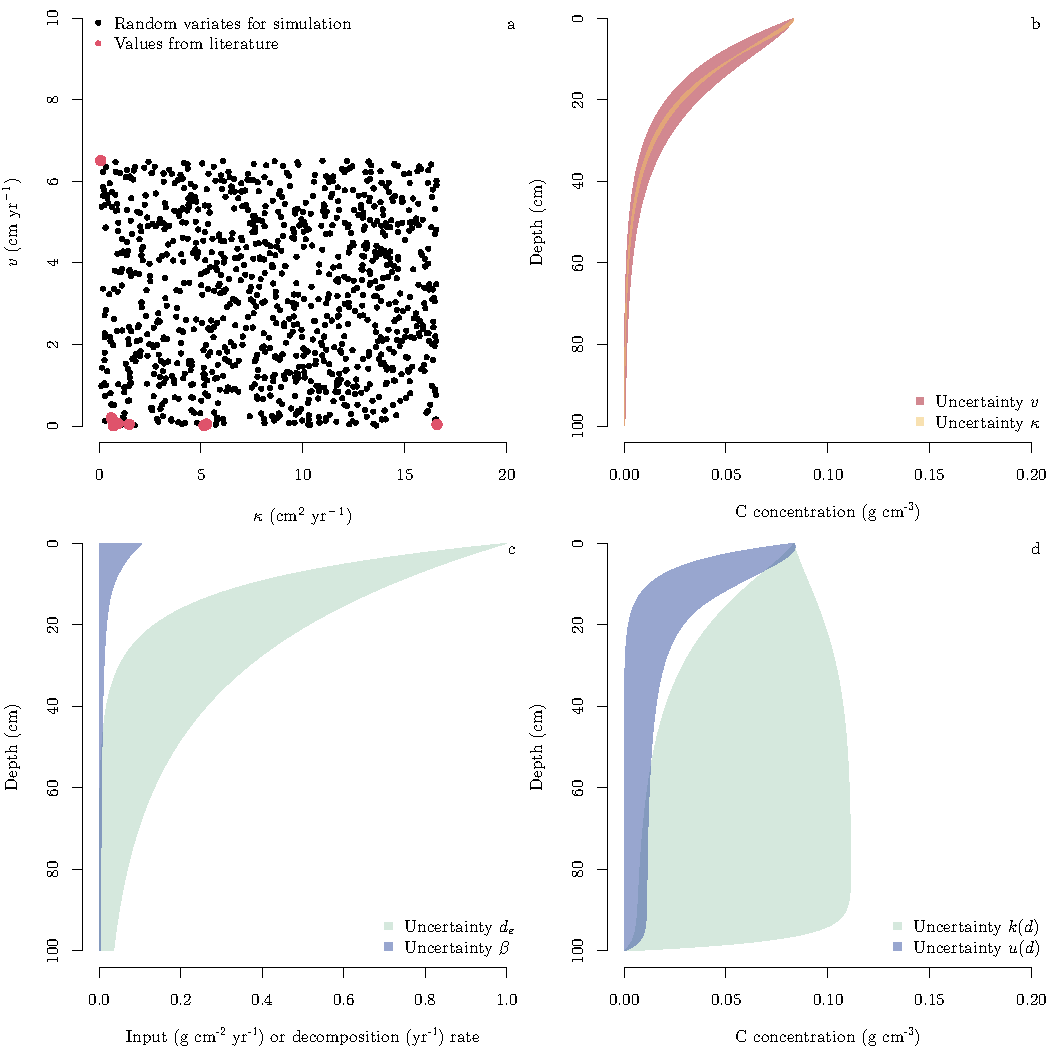
\includegraphics[width=\textwidth]{Figures/uncertainty.pdf} % requires the graphicx package
   \caption{Uncertainty analysis based on the components of equation \eqref{eq:simpleCase} using a Monte Carlo uncertainty approach in which 1000 random variates of model parameters were chosen from a uniform distribution $U$. (a) Set of 1000 random variates of parameters $\kappa \sim U(0.09, 16.58)$ and $v \sim U(0.01, 6.51)$, and the set of values available from the literature (Table \ref{tab:Models}). (b) Prediction uncertainty in carbon concentration due to uncertainty in $\kappa$ and $v$. (c) Uncertainty in the distribution of root inputs ($u(d)$) due to uncertainty in parameter $\beta \sim U(0.9, 1.0)$, and uncertainty in decomposition rate distribution ($k(d)$) due to uncertainty in parameter $d_e \sim U(10, 100)$. (d) Prediction uncertainty in carbon concentration due to uncertainty in root input distribution and decomposition rate distribution. }
   \label{fig:uncertainty}
\end{figure}

Overall, the sensitivity analysis presented in Figures \ref{fig:AdvectionDiffusion} and \ref{fig:rootDecomp}, and the uncertainty analysis in Figure \ref{fig:uncertainty} indicate that the vertical distribution of root inputs and decomposition play a larger role in determining the shape of soil carbon profiles than transport processes represented as diffusion and advection. 

\section{Assessing C sequestration and the fate of new C inputs}
\subsection{Fate, transit time, and carbon sequestration in the subsoil}
In the context of climate change mitigation, we are generally interested in evaluating the capacity of soils for storing carbon at relevant timescales associated with management and policy outcomes. In many cases, we are interested in comparing different soils; and in other cases, we are interested in evaluating the effectiveness of different soil management practices. In any case, we need to use appropriate metrics to evaluate the environmental benefit of carbon sequestration. 

If we aim at promoting soil C sequestration, it is then important to analyze the fate of new inputs entering the soil, assess for how long the new carbon remains stored, and how much warming can be avoided while the C is stored \citep{Sierra2021BGS, Crow2022}. For this purpose, we can use the following metrics: fate, transit time, and carbon sequestration, which are mathematically defined as follows.

For a compartmental system in equilibrium, where carbon inputs are balanced with C losses, the fate of C entering at a time $t_0$ can be obtained as a function that predicts the mass of C remaining in the soil at time $t$, thus we define $\tau = t- t_0$, and  
\begin{equation} \label{eq:m}
\bm{m}(\tau) = e^{\tau \mathbf{B}} \ \bm{u},
\end{equation}
as in \citet{Sierra2021JE}, where $\bm{m}(\tau)$ is a vector with the mass remaining for each compartment. This mass remaining is related to the transit time of carbon, which is defined as the time it takes carbon atoms to pass through the entire network of compartments until C leaves the soil system \citep{Bolin1973, Manzoni2009JGR, Sierra2018JAMES}. The transit time distribution of carbon can be expressed as \citep{Metzler2018MG}
\begin{equation} \label{eq:transitTime}
f_T(\tau) = -\bm{1}^{\top} \ \mathbf{B} \ e^{\tau \mathbf{B}} \frac{\bm{u}}{\Vert \bm{u} \Vert},
\end{equation}
and represents the relative proportion of carbon leaving the system at a time $\tau$. In soils, transit time distributions generally have a long tail, indicating that most carbon entering soils are respired quickly but small proportions can stay for long times \citep{Sierra2018GBC}. 


Carbon Sequestration (CS) is the storage of a certain amount of carbon over a certain period of time. It evaluates the fate of new inputs entering the soil integrated over a time horizon. The amount of sequestration quantified by the CS metric depends on both the amount of inputs entering the soil and the time it takes this carbon to return to the atmosphere in the form of respiration. This amount of time is proportional to the transit time of carbon. 


%\subsection{The transit time distribution as a tool to assess C sequestration}
For a compartmental system at equilibrium, CS can be obtained as \citep{Sierra2021BGS}
\begin{equation} \label{eq:CS}
 \mathrm{CS}(t) = \int_{t_0}^t \Vert e^{\tau \ \mathbf{B}} \ \bm{u} \Vert \mathrm{d} \tau,
\end{equation}
which is the integral of the total amount of mass remaining in the soil from a cohort of inputs entering at $t_0$.

If a particular transport-decomposition model can be discretized and expressed as a compartmental system following standard numerical methods \citep{LeVeque2007, Lanczos}, one can use equations \ref{eq:m}, \ref{eq:transitTime}, and \ref{eq:CS} to quantify the fate, transit time and CS of a particular soil and compare results with those from another soil, or with the outcomes of different forms of management. 

Alternatively, $\bm{m}(t)$ and $f_T(\tau)$ can be obtained using impulse response experiments with existing transport models that are difficult to express as a compartmental system \citep{Thompson1999, Metzler2018MG}. The approach consists of running a model until reaching equilibrium, and at this point add a pulse of carbon and observe the mass remaining of the pulse over time, which is an approximation to $\bm{m}(t) $. One can also observe the respiration flux after the addition of the pulse, which is an approximation to the transit time distribution $f_T(\tau)$ \citep{Metzler2018MG}. The results from pulse-response experiments should provide very valuable information to assess the fate of new inputs entering the soil and whether they remain for relevant periods of time. 

%the transit time distribution can be obtained by the expression \citep{Metzler2018MG}
%\begin{equation} \label{eq:transitTime}
%f(\tau) = -\bm{1}^{\top} \ \mathbf{B} \ e^{\tau \mathbf{B}} \ \bm{u}
%\end{equation}

%\subsection{Example: a pulse response experiment with the COMISSION model}

\subsection{Numerical example}
In the previous example, we saw that transport, decomposition, and lateral root inputs play an important role in determining the shape of soil C profiles at equilibrium. We evaluate now with an example how fast/slow transport, combined with fast/slow decomposition in soil profiles can affect the fate, transit time and carbon sequestration of a soil. Our aim is to assess the fate of new carbon inputs and whether they remain in soil for timescales relevant for climate change mitigation.

Given that our previous example showed that diffusion plays a minor role in comparison to advection for moving carbon downwards, we set a fixed value of $\kappa = 1$ cm$^2$ yr$^{-1}$ and varied the values of $v$. For simulations with fast transport, the values were $v = 5$ cm yr$^{-1}$, and for simulations with slow transport $v = 0.1$ cm yr$^{-1}$. Decomposition rates were considered fast with values of $k_0 = 1$ yr$^{-1}$ and slow with $k_0 = 0.1$ yr$^{-1}$ at the surface (Table \ref{tab:simulationSetup}) and declining with depth according to equation \ref{eq:kd}. In all simulations, we considered a root input profile with an intermediate value of $\beta = 0.95$, i.e. not too shallow nor too deep roots. 

% Requires the booktabs if the memoir class is not being used
\begin{table}[h]
   \centering
   \caption{Parameters used and results obtained for simulations evaluating the effect of transport and decomposition on the fate, transit time and carbon sequestration of new inputs. Tf--Df: transport fast, decomposition fast; Tf--Ds: transport fast, decomposition slow; Ts--Df: transport slow, decomposition fast; Ts-Ds: transport slow, decomposition slow.}
   \begin{tabular}{@{} lcccr @{}} % Column formatting, @{} suppresses leading/trailing space
%\begin{tabular}{l|r|r|r|r}
\toprule
 & Tf--Df & Tf--Ds & Ts--Df & Ts--Ds\\
\midrule
$\kappa$ (cm$^2$ yr$^{-1}$) & 1.000 & 1.000 & 1.000 & 1.000\\
$v$ (cm yr$^{-1}$) & 5.000 & 5.000 & 0.100 & 0.100\\
$k_0$ (yr$^{-1}$) & 1.000 & 0.100 & 1.000 & 0.100\\
$\beta$ & 0.950 & 0.950 & 0.950 & 0.950\\
Proportion remaining after 1 yr & 0.449   & 0.914 & 0.424  & 0.875\\
Proportion remaining after 10 yr & 0.002  & 0.480 & 0.001 &  0.392 \\
Proportion remaining after 50 yr & 0.000  & 0.000 & 0.000  & 0.022 \\
Mean transit time (yr) & 1.333  & 9.699 & 1.217 & 11.498 \\
Median transit time (yr) & 0.859  & 9.444 & 0.799  & 7.096 \\
CS($t \to \infty$) & 16.028 & 363.721 &12.587 &133.416 \\
\bottomrule
\end{tabular}
   \label{tab:simulationSetup}
\end{table}

Simulation results showed that most C inputs entering at any given time only stay in the soil a few years, and only under slow decomposition, some C may remain for a few decades (Figure \ref{fig:Mt}, Table \ref{tab:simulationSetup}). Decomposition rates seem to play a stronger control on the fate of C inputs than vertical transport rates. Under fast decomposition, most carbon was lost in 5 years independently from transport velocity, and very small proportions travelled through the soil profile because the carbon was decomposed before it had a chance to move downwards. Under slow decomposition and fast transport, some carbon is preserved longer because it decomposes at slower rates at deeper layers, but eventually this transported carbon is also decomposed in a few decades (Figure \ref{fig:Mt}).

\begin{figure}[htbp]
   \centering
   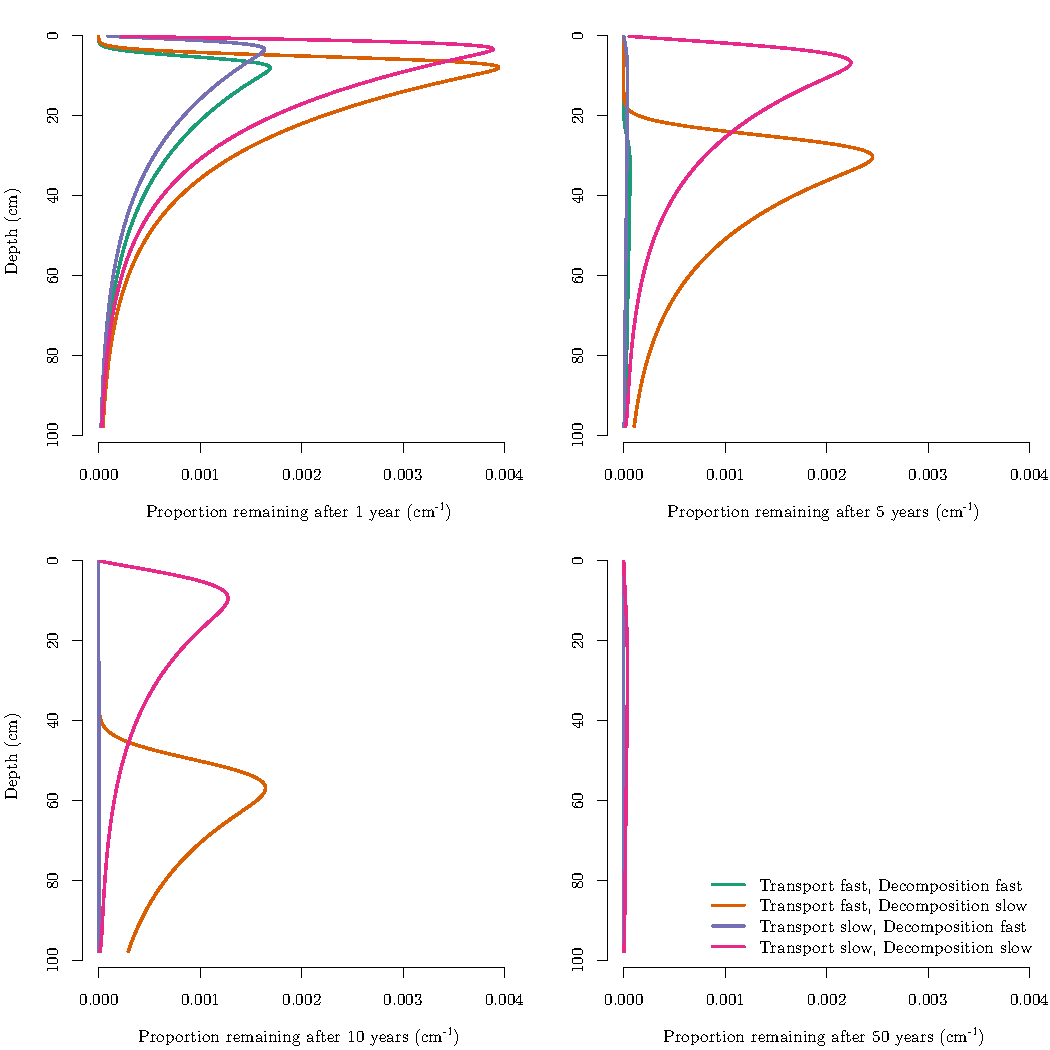
\includegraphics[width=\textwidth]{Figures/Mt.pdf} % requires the graphicx package
   \caption{Proportion of C remaining in a soil profile of an amount of lateral inputs entering the soil at $t=0$ represented with equation \ref{eq:ud} with $\beta = 0.95$. After 50 years most of the carbon that entered at $t=0$ is not present in the soil, even for the scenario with slow transport and decomposition rates. }
   \label{fig:Mt}
\end{figure}

The transit time distribution of C through the entire soil profile for these different simulations showed that the large majority of C entering the soil at any given time is lost within the first year (Figure \ref{fig:transitTime}a). Fifty percent of the C that enters the soil is lost in 0.86 years in the scenario with fast decomposition and fast transport, while in the scenario with slow decomposition and fast transport 50\% of the new carbon is lost in 9.4 years (Table \ref{tab:simulationSetup}). The slow decomposition scenarios showed a very different tail in the transit time distribution compared to the fast decomposition scenarios, with a larger proportion of carbon staying for longer times under slow decomposition. Therefore, the mean transit time is influenced by these long tails, with the mean transit time in the fast transport slow decomposition scenario of 1.3 years, and 11.5 years in the slow transport slow decomposition scenario (Table \ref{tab:simulationSetup}a). Despite slow decomposition however, most of the new inputs do not stay for timescales beyond a few decades at the maximum. 

At steady-state, significantly more carbon is stored in the case of slow decomposition, particularly in the scenario of fast transport and slow decomposition (Figure \ref{fig:transitTime}b). However, to reach this large steady-state C concentrations, very long timescales of carbon accumulation are required. According to the transit time distributions, very small amounts of new C inputs remain in the long-term, therefore it would take a considerably long time (beyond decades) to reach these steady-state C values. 

\begin{figure}[htbp]
   \centering
   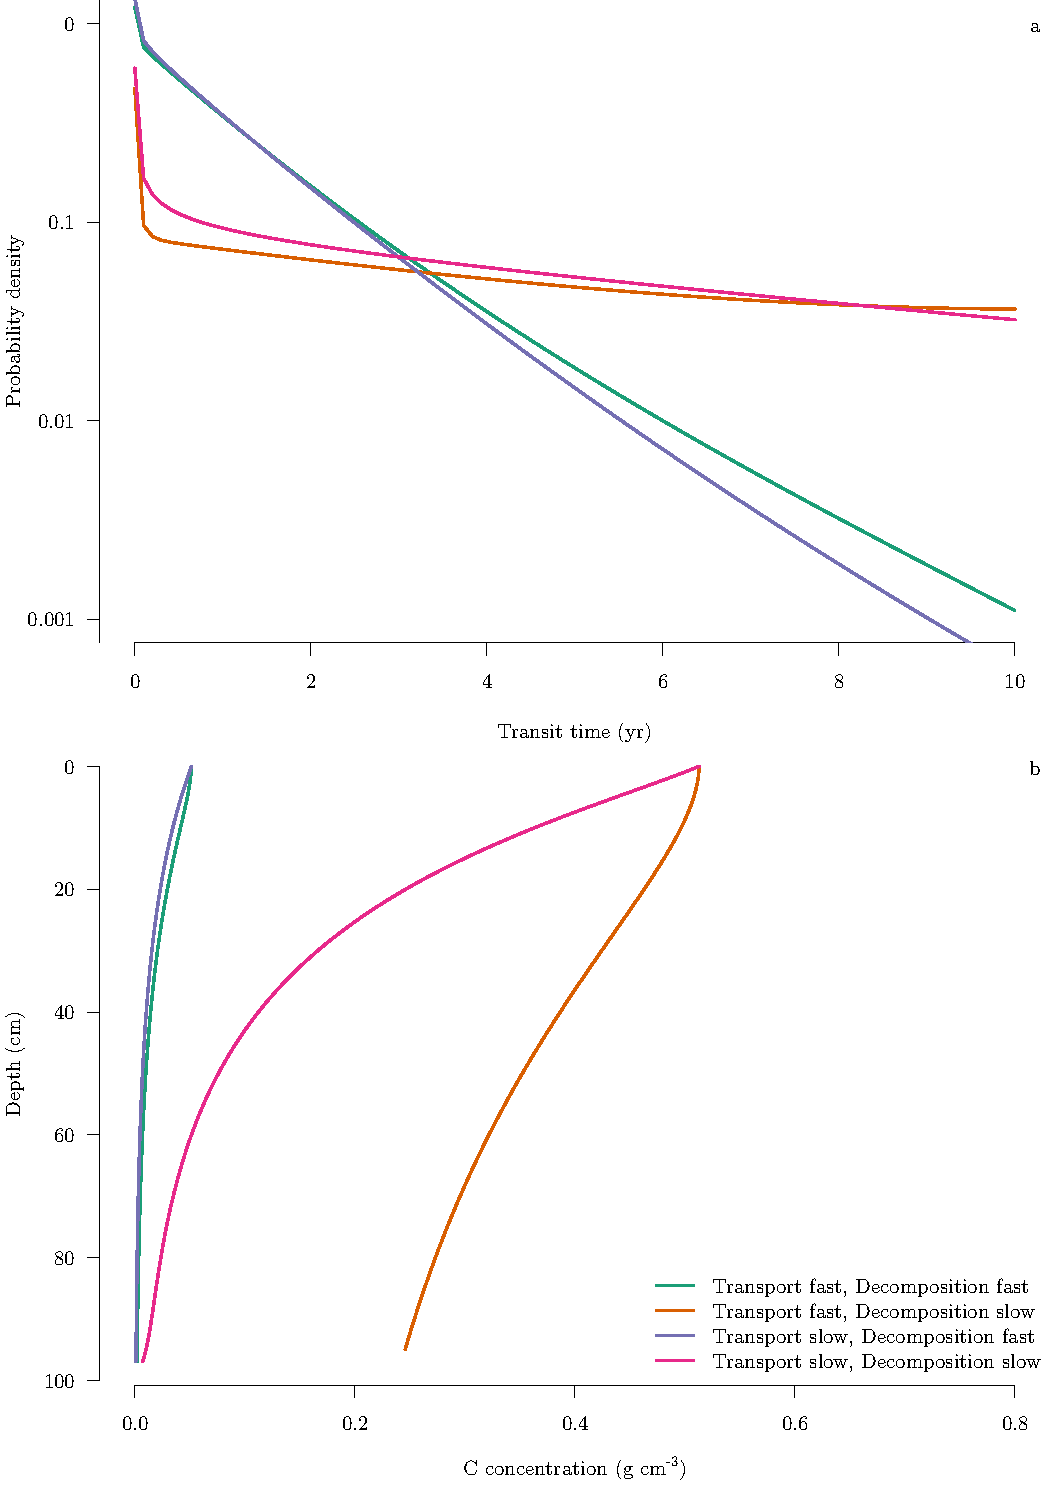
\includegraphics[width=\textwidth]{Figures/transitTimes.pdf} % requires the graphicx package
   \caption{(a) Transit time distributions for four different scenarios of transport and decomposition in the subsoil. These distributions represent the proportion of C leaving the soil system at different times since the C entered the soil. Note the logarithmic y axis. (b) Values of C concentration along the depth profile at steady-state.}
   \label{fig:transitTime}
\end{figure}

\section{Empirical evidence from soil profiles}
The two numerical examples from the previous section suggest that (i) the change of soil C with depth is largely influenced by the difference between root inputs and decomposition, and to a lesser degree by vertical transport processes such as diffusion and advection; (ii) most new carbon inputs entering the soil do not remain stored for long timescales. In the following section, we will explore global-scale datasets of soil C profiles to test whether these theoretical model predictions have empirical support on observations.

\subsection{The shape of the vertical C profile across regions}
The International Soil Radiocarbon Database (ISRaD) is a comprehensive and well curated collection of soil carbon and radiocarbon data  \citep{Lawrence2020}. We used version 1.7.8 of the database and extracted information on soil C concentration with depth down to 1 m. Data from 600 individual profiles were grouped by K\"oppen-Geiger climate zones \citep{Beck2018} and averaged by 1 cm depth increments. Volcanic soils (classified as such in the field) were treated as a separate group given their distinct vertical C profile. A mass-preserving spline function (equal-area quadratic smoothing spline) was applied to each profile to account for the varying depth intervals in which samples across profiles were taken \citep{Ponce1986,Bishop1999}. This spline function interpolates C concentration for a continuum of depths, i.e. an approximation to the function $x(d)$ for each of the groups (Figure \ref{fig:Cprofiles}). 


\begin{figure}[htbp]
   \centering
   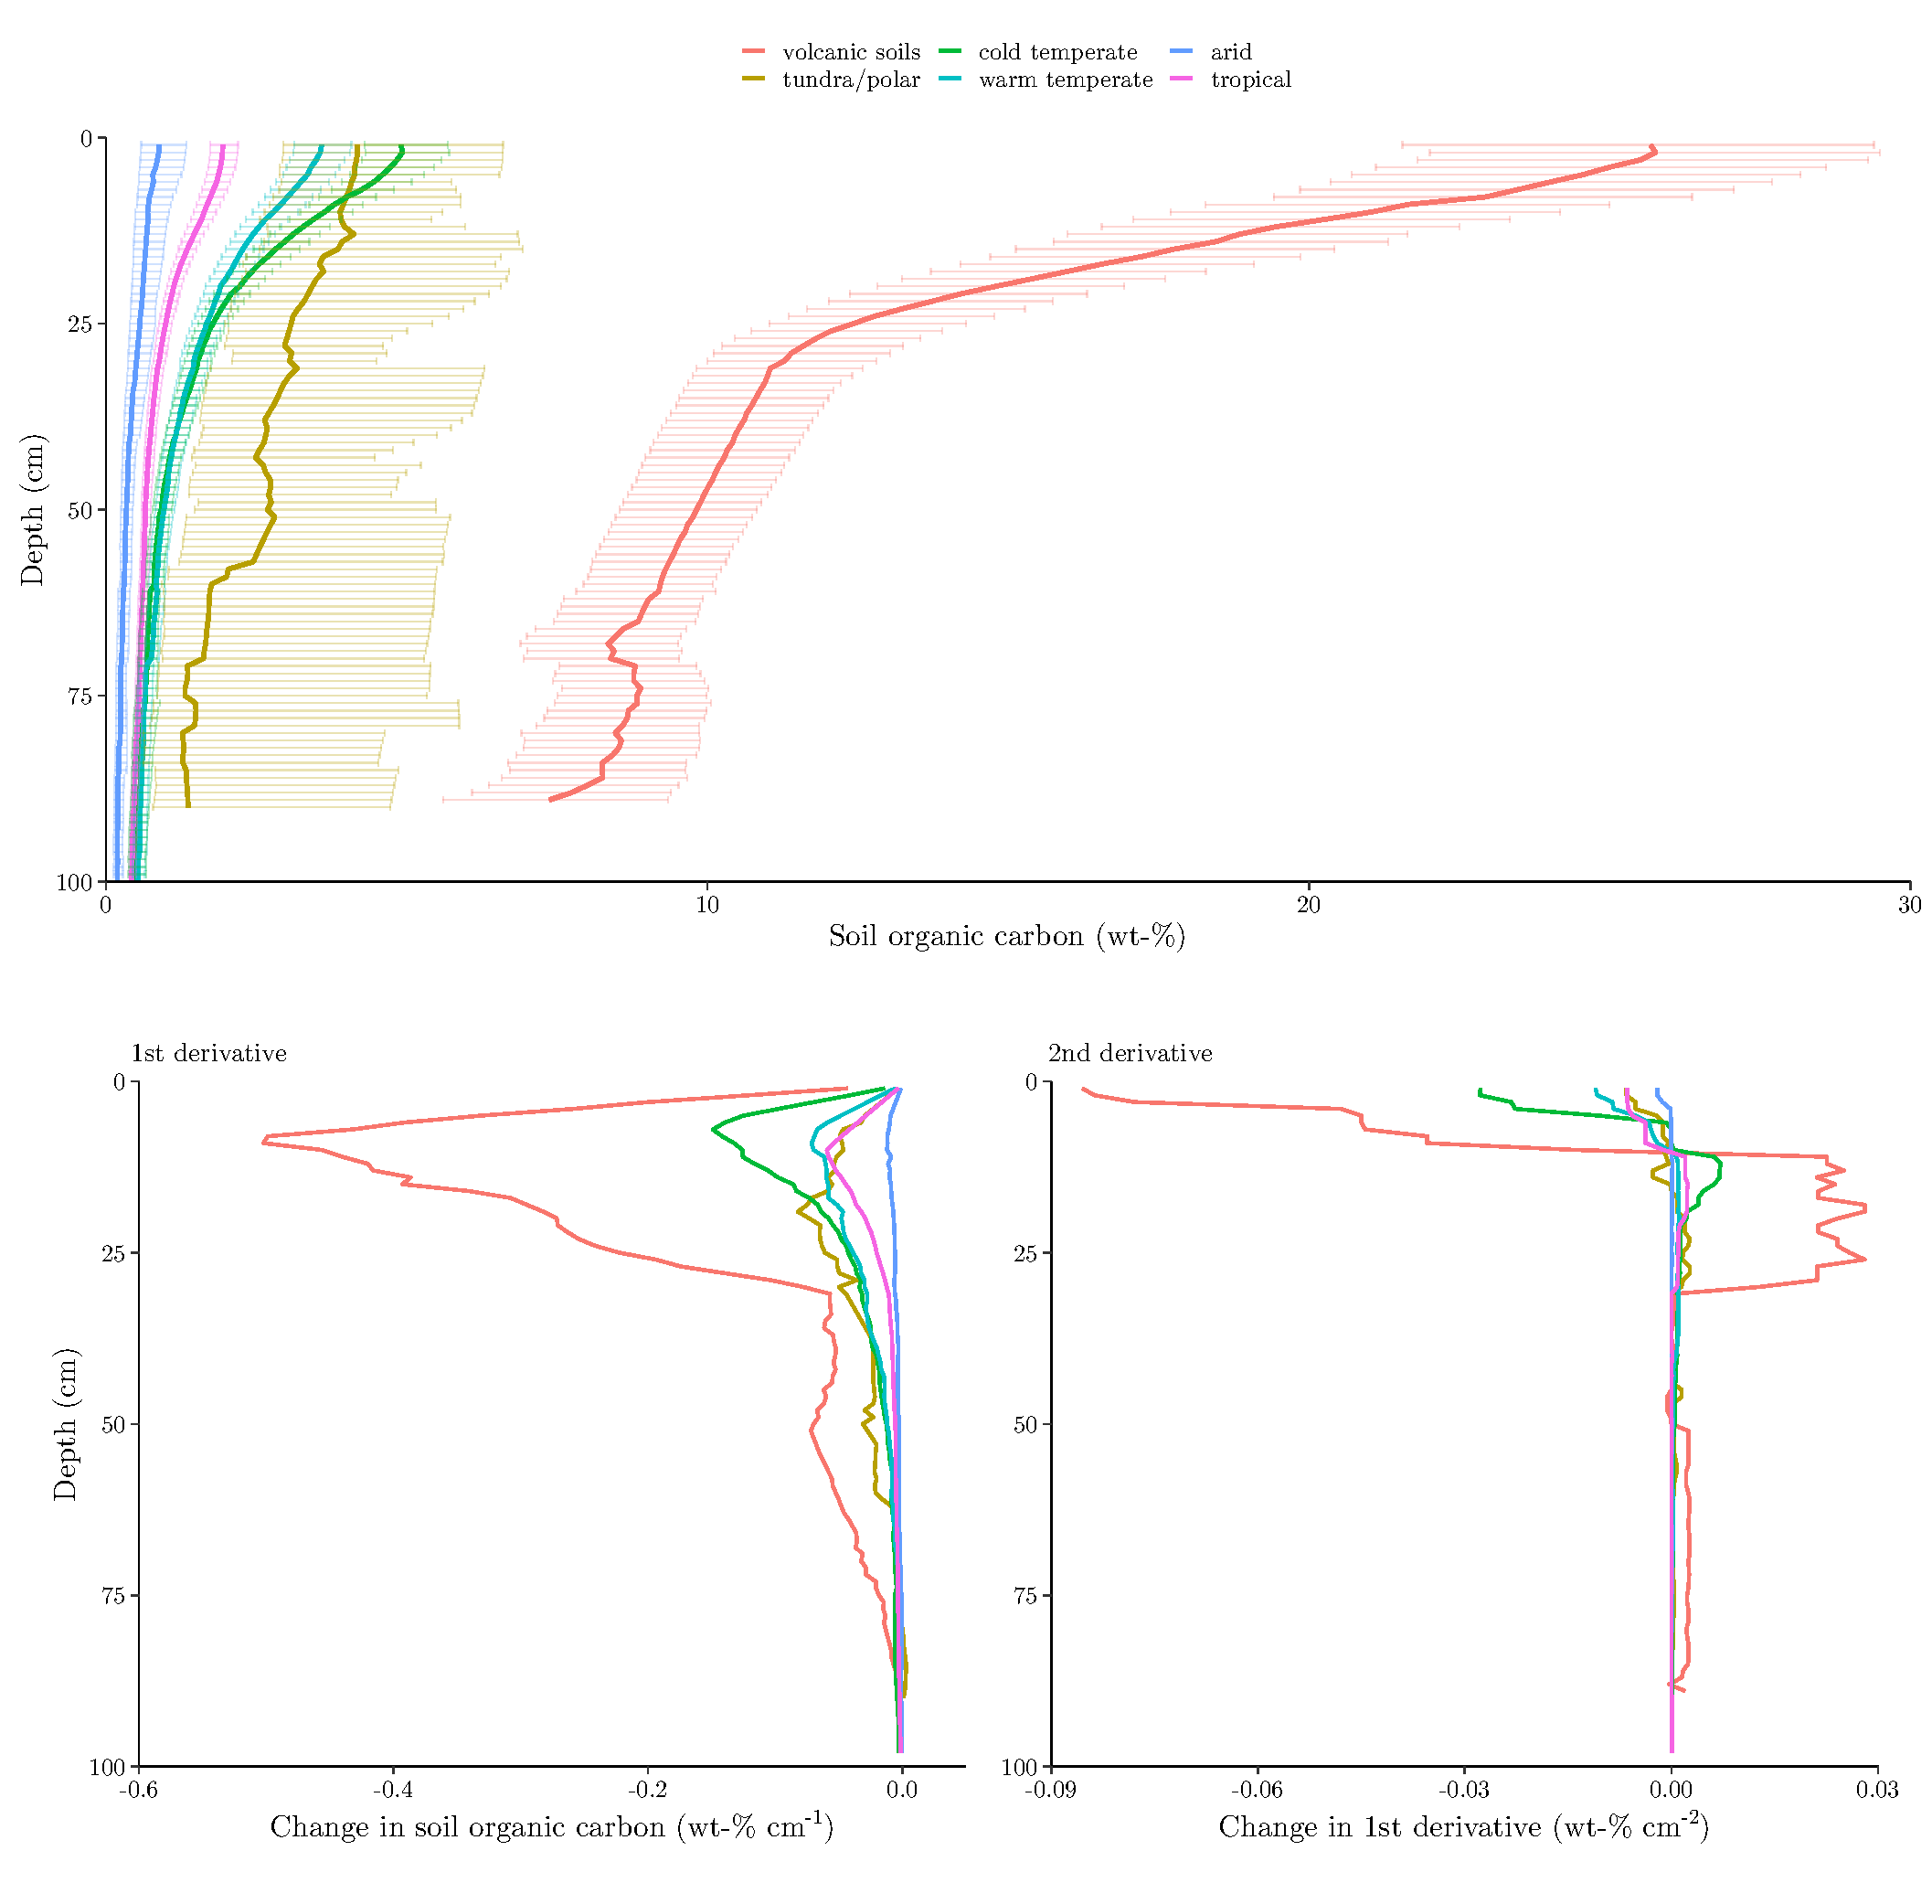
\includegraphics[width=\textwidth]{Figures/profiles.pdf} % requires the graphicx package
   \caption{Soil carbon concentrations with 1st and 2nd derivatives with respect to depth obtained from the International Soil Radiocarbon Database, with data from 600 profiles aggregated by biogeographical regions. Thick lines for each group represent the mean across available observations and fitted to a spline curve. Horizontal lines represent standard deviation across available observations. }
   \label{fig:Cprofiles}
\end{figure}

Soil carbon decreased rapidly with depth in most soil profiles reaching values close to zero at 1 m depth (Figure \ref{fig:Cprofiles}), with the exception of soils from tundra/polar regions and volcanic soils, which still contain relatively large quantities of C at 90 cm depth. Please note that these values are reported as concentrations with respect to mass of soil. Bulk density data is not commonly reported for individual profiles and much less for individual depth horizons. Therefore, comparisons with the simulation experiments from previous sections must be done only with respect to qualitative aspects and not with respect to quantitative values. 

%\begin{figure}[htbp]
%   \centering
%   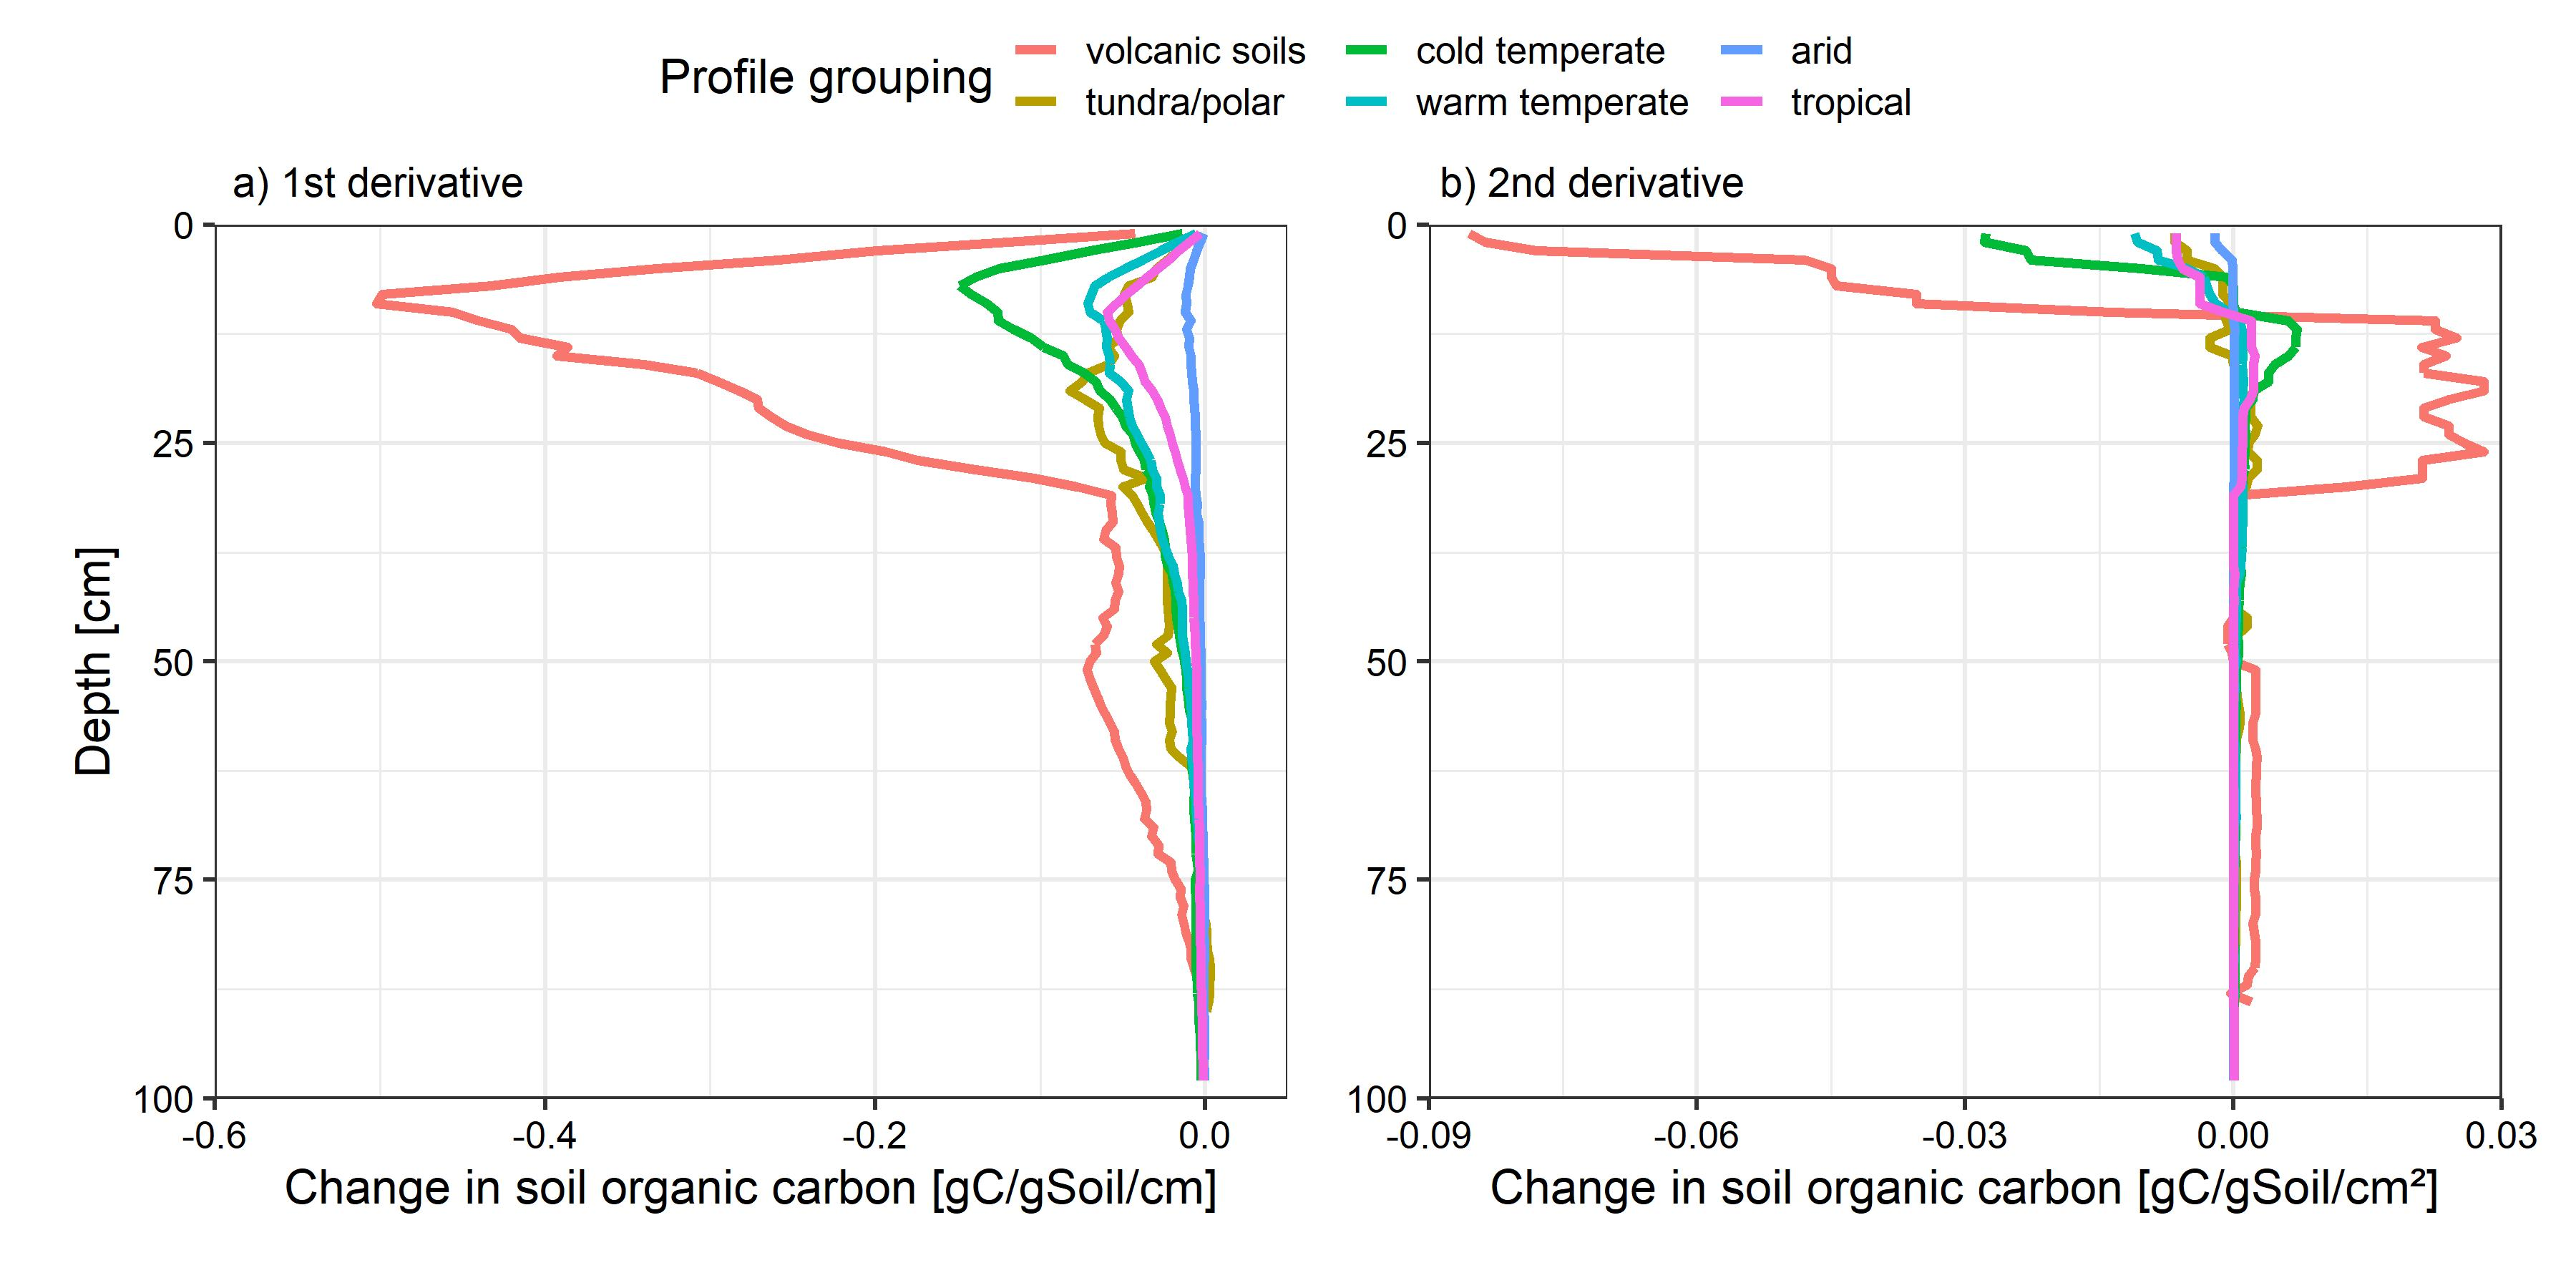
\includegraphics[width=\textwidth]{Figures/ISRaD_msp_14C_SOC_climate_depth_deriv_2023-03-13.jpeg} % requires the graphicx package
%   \caption{First and second derivative of soil C profiles extracted from ISRaD and grouped by biogeographical region, with the exception of volcanic soils.}
%   \label{fig:Derivatives}
%\end{figure}

The first derivative of soil C concentrations with respect to depth ($\partial x(d)/ \partial d$, Figure \ref{fig:Cprofiles})  was negative for all groups, indicating that soil C always decreases with depth for these aggregated profiles. This is in  agreement with our previous simulations in which the first derivatives were always negative. We observed for all groups a peak in the first derivative where it reaches a maximum negative value, indicating that soil C decreases more strongly at some intermediate depth between 10 and 20 cm (Figure \ref{fig:Cprofiles}). According to equation \ref{eq:simpleCase}, a maximum negative value of the first derivative can only occur at depths where the microbial decomposition flux ($k(d) x(d)$) has its maximum value, i.e. when microbes are consuming the maximum amount of carbon possible.

The value of the first derivative had the largest values overall for volcanic soils, and the lowest values for arid soils. In both cases decomposition rates may be slow compared to other soils; in volcanic soils the presence of amorphous non-crystalline surfaces promote sorption of organic matter to minerals and therefore slow decomposition and strong C accumulation \citep{Marin-Spiotta2011, Crow2015}; in arid soils low moisture availability leads to slow decomposition rates, but also low primary productivity leads to low carbon stocks \citep{Moyano2013, Sierra2015JAMES}. Therefore, negative values of the first derivative are strongly dependent on the C stocks ($x(d)$), and to a lesser extend on the decomposition rate ($k(d)$). The decomposition rate obviously plays a major role in determine the size of the C stock in conjunction with the input fluxes at depth, but the rate of decline of C with depth is mostly influenced by the resulting C stock. In addition, the last term of equation \ref{eq:simpleCase} also reveals that for systems with slow advection velocities $v$ approaching zero, small differences between lateral inputs and decomposition may be amplified. In other words, the large values of the negative derivative for the volcanic soils may be the result of very low advective movement of DOC, amplifying small differences between lateral inputs and decomposition.

Overall, the data from soil C profiles aggregated by regional groups and volcanic soils provide evidence supporting the idea that vertical transport may play a secondary role in determining the rate of soil C decrease with depth. The difference between lateral root inputs and decomposition may play a primary role in determining the shape of soil C profiles, and this difference may be amplified at low advection velocity rates. Diffusive movement of soil C seems to play a small role in these aggregated groups, something suggested by the low values of the second derivative (Figure \ref{fig:Cprofiles}); however, diffusion may have some control on the peak of C decrease found close to the surface in these profiles. 

\subsection{Transit times of C from vertical profiles}
Using data from ISRaD and a dataset on root input profiles, \citet{Xiao2022} obtained estimates of mean ages and mean transit times for soil C profiles at the global scale. The global averages revealed that mean transit times of C are always younger than the mean age of C stored at all soil depths (Figure \ref{fig:AgeTTprofiles}). In other words, despite the C stored in the soil being hundreds to thousands of years old, the C respired is only a few years to decades old. This result is consistent with our transit time simulations that showed mean transit times of only a few years (Figure \ref{fig:transitTime}, Table \ref{tab:simulationSetup}). However, the actual values of mean transit time obtained from the data are actually much higher than those from the model results. This is to be expected given that the model used for the example only considered one single pool with a relatively fast decomposition rate, but in reality soil carbon is highly heterogeneous and a significant proportion of its total carbon cycles at much slower rates, which would contribute to longer transit times.  In addition, sorption of OM to mineral surfaces may increase with depth, making the overall decomposition of C at depth more limited \citep{Ahrens2020}. Nevertheless, model simulations and observations agree in that new C inputs to soil only remain stored in timescales of years to decades. 

Fast mean transit times were observed for tropical forest, grassland and cropland soils, while long transit times in the order of decades to centuries were only observed for tundra and boreal forest soils (Figure \ref{fig:AgeTTprofiles}). These results are consistent with the idea that low temperatures and energy limitation may play a significant role in controlling the transit time of C at the biome level \citep{Lu2018, Xiao2022, Sierra2023PTRS}, with fast transit times in warm regions and longer transit times in cold high-latitude regions.

Because transit times are directly related to Carbon Sequestration CS (equations \ref{eq:transitTime} and \ref{eq:CS}), we expect only tundra and boreal forest soils to store C in the subsoil at timescales relevant for climate change mitigation, i.e. in the order of decades to centuries. In fact, previous studies have found that a large proportion of carbon used by microorganisms in the subsoil is recent and does not contribute to C stabilization in the subsoil \citep{Balesdent2018, Scheibe2023}. Therefore, we would expect lower values of CS for tropical forests, grasslands and cropland soils in comparison with boreal forests and tundra soils. 
However, it is important to keep in mind that productivity in these high-latitude regions is relatively low compared to temperate and equatorial latitudes \citep{Xiao2023}. CS as defined in equation \ref{eq:CS} accounts for this trade-off between the amount of inputs and its transit time through the soil, and it can be used to more specifically assess the climate mitigation potential of specific amounts of C added to the soil.

\begin{figure}[htbp]
   \centering
   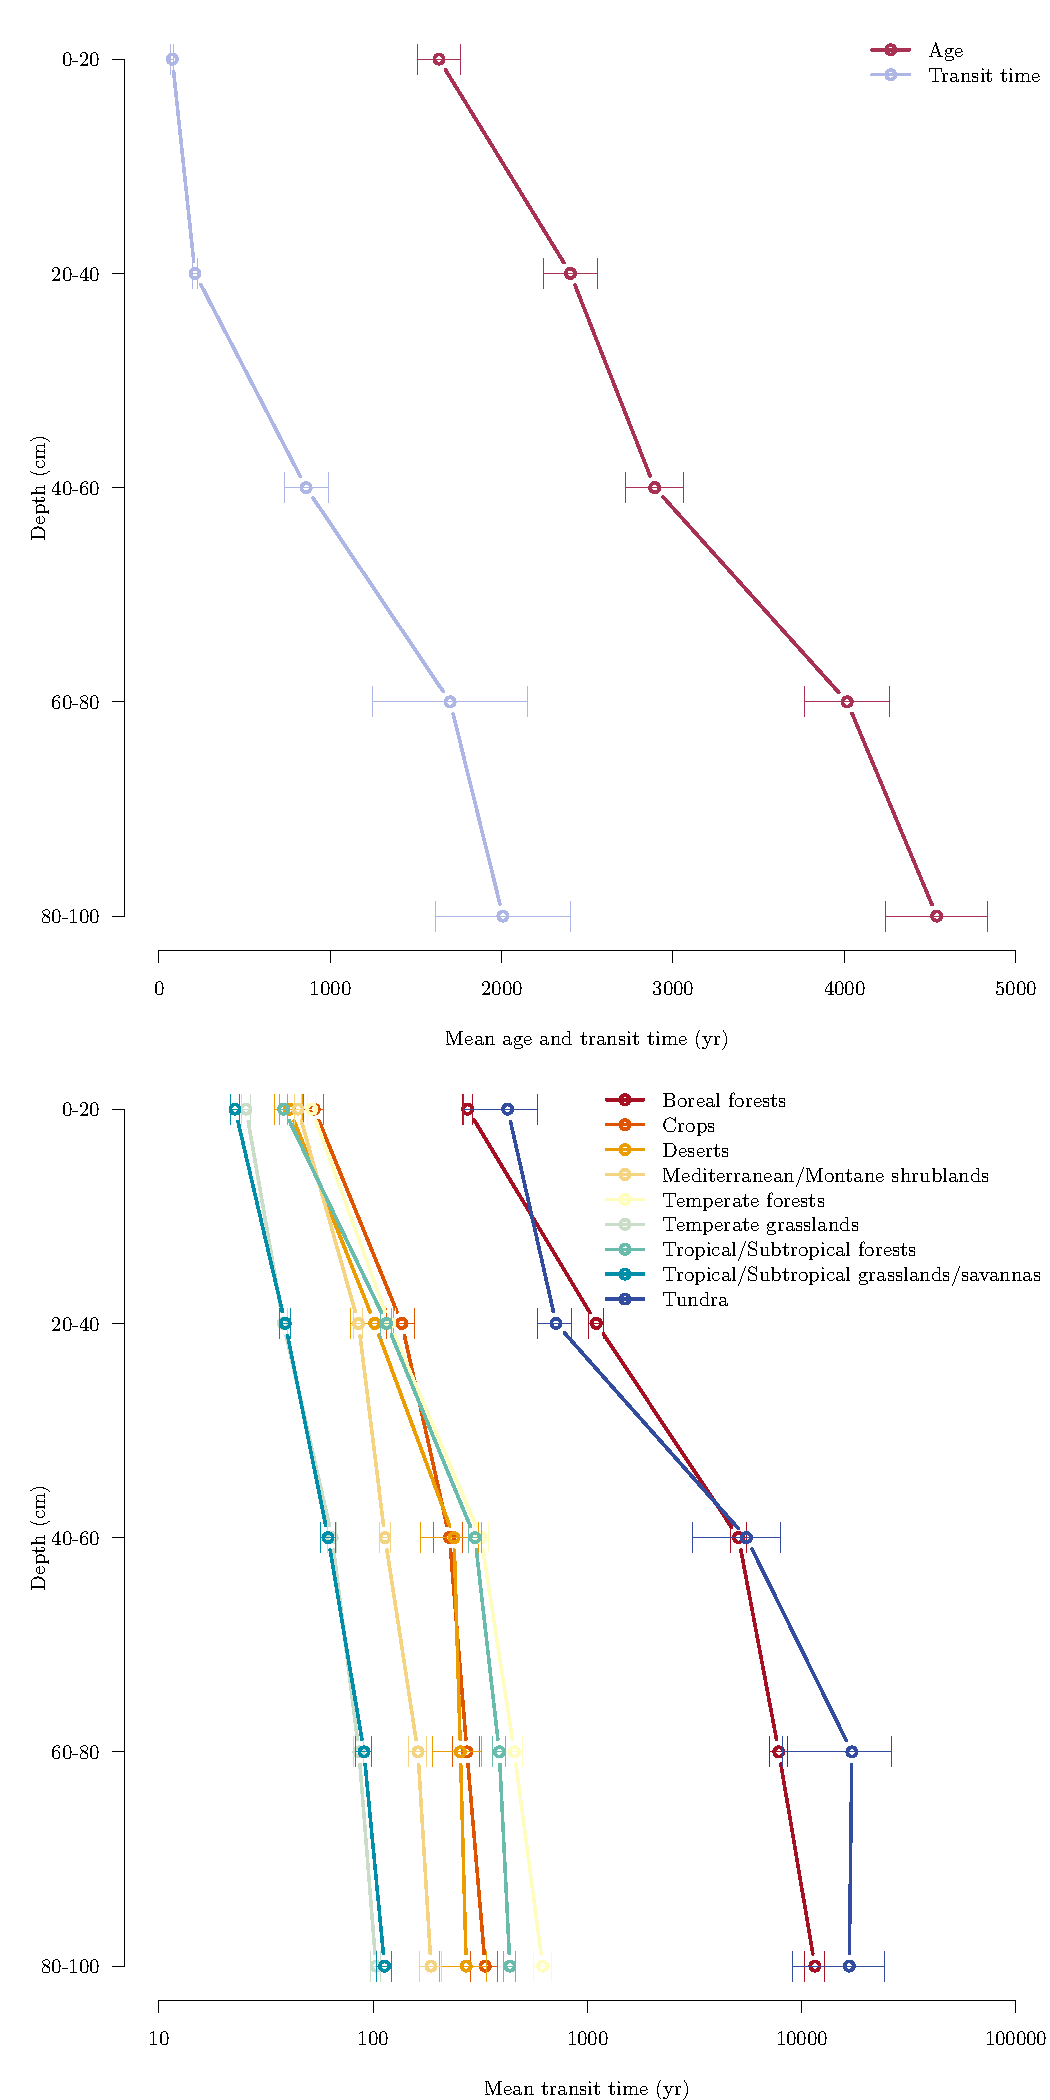
\includegraphics[scale=0.65]{Figures/biomeTT.pdf} % requires the graphicx package
   \caption{Estimates of mean age and mean transit time of carbon based on measurements of root inputs and soil radiocarbon obtained from ISRaD. The left panel shows global-scale average values of mean age and mean transit time. The lower panel shows averages of mean transit time aggregated by biome.}
   \label{fig:AgeTTprofiles}
\end{figure}

\section{Implications for soil C management}
Our analysis of a general model of soil C profile formation, together with the analysis of observations of soil carbon concentrations and transit times, provide relevant insights that can inform land management for carbon sequestration and climate change mitigation. 
Even though current observations show that C concentrations decrease strongly with depth in most soils and new C inputs transit relatively fast, there are potentials to increase C storage with depth and increase the transit time of carbon across the entire profile. 

%Data on C concentrations and their change with depth in global soil profiles (Figures \ref{fig:Cprofiles} and \ref{fig:Derivatives}) show that C stocks decline strongly with depth for most soils. 
If soils would be managed to increase subsoil C storage, the change of C concentrations with depth should be less dramatic and change less with respect to topsoil (Figure \ref{fig:managementObjective}). From equation \ref{eq:firstDeriv}, it can be inferred that a management objective could be framed in terms of keeping the first derivative of C concentration with respect to depth close to zero, so the storage of carbon in subsoil remains relatively similar to levels in topsoil. Using the model of constant advection and diffusion coefficients at steady-state (equation \ref{eq:firstDeriv}), we can frame this management objective as 
\begin{equation}
\frac{\partial x(d)}{\partial d} = \frac{\kappa}{v} \frac{\partial^2 x(d)}{\partial^2 d} + \frac{g(d)}{v} = 0,
\end{equation} 
and because the derivative of a constant value of zero is equals to zero, the second derivative term vanishes from this equation and the management objective reduces to
\begin{equation} \label{eq:objective}
 \frac{g(d)}{v} = 0.
\end{equation} 


\begin{figure}[htbp]
   \centering
   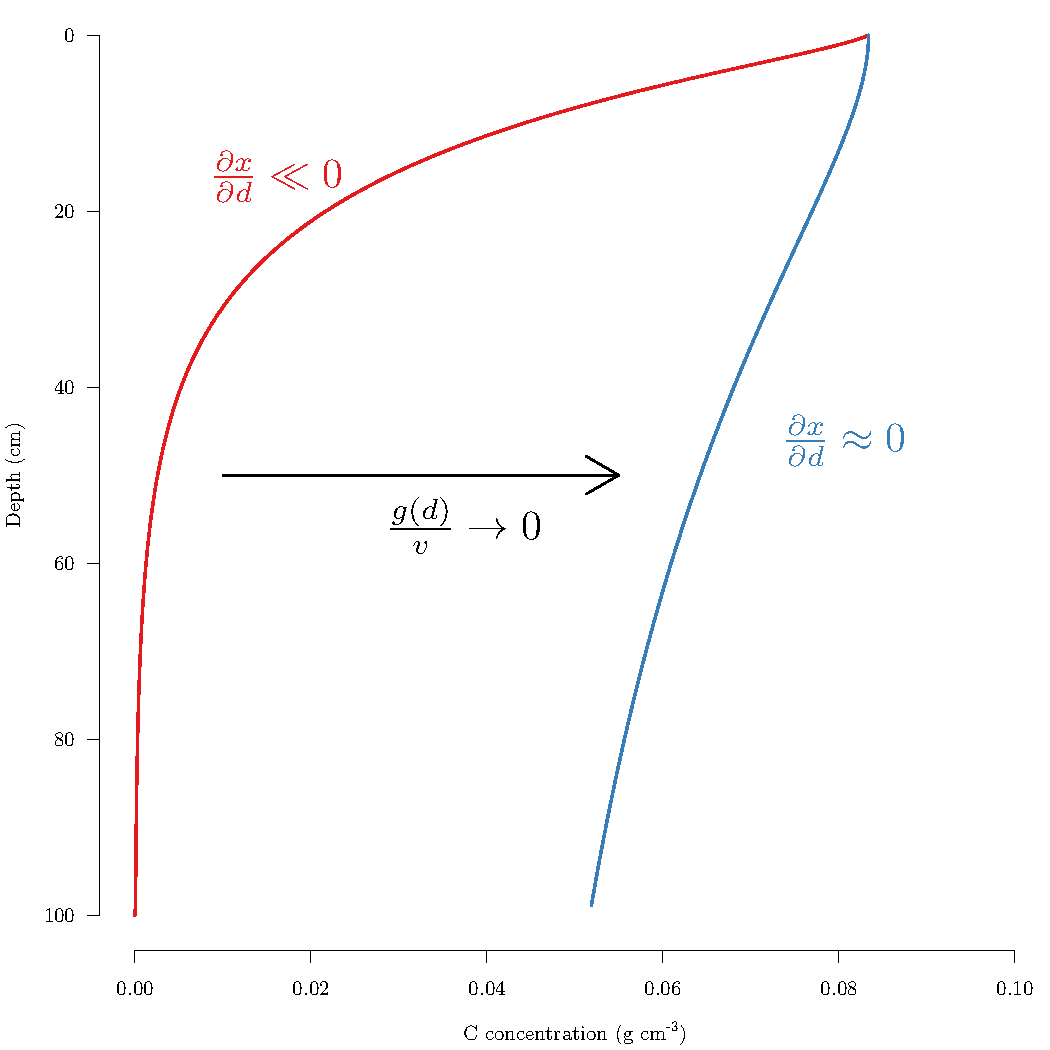
\includegraphics[width=\textwidth]{Figures/managementObjective.pdf} % requires the graphicx package
   \caption{Graphical example for defining a management objective to increase C storage in the subsoil. By decreasing the ratio $g(d)/v$ as close to zero as possible, the decrease of C concentration with depth is less steep and more carbon can be stored in the subsoil. For this example, advection velocity was increased from 1 to 100 cm yr$^{1}$.}
   \label{fig:managementObjective}
\end{figure}

This equation suggest that an effective way to achieve the goal of increasing C storage in the subsoil would be through increasing advective transport of C from top to subsoil; i.e. increasing values of $v$ so the ratio of equation \ref{eq:objective} approaches zero (Figure \ref{fig:managementObjective}). Provided C inputs are high, their vertical advective movement should contribute to increase total carbon storage. In other words, even though vertical C transfer does not seem to play a significant role in explaining current data on soil C profiles, management activities could be implemented to increase vertical C transfers to horizons where it can be stabilized on available mineral surfaces \citep[cf.][]{Ahrens2020, Georgiou2022} and protect it from decomposition. Equation \ref{eq:firstDeriv} also suggest that a small difference between C inputs and decomposition across all depths ($g(d) \approx 0$) helps to decrease the gradient of C decline with depth. For example, exogenous amendments of organic matter with low decomposition rates could help to reduce this difference and reduce C decline with depth. There may be many other ways to achieve this management goal, and a challenge for future research would be to test this theoretical prediction through innovative experiments.

Equation \ref{eq:objective} also suggests that changes in particle diffusion have little or no effect in contributing to increase carbon storage in the subsoil. This may imply that the diffusive mixing of carbon due to tillage plays no relevant role for increasing carbon in the entire profile. 

\section{Summary and conclusions}
We reviewed the main processes that contribute to the formation of soil C profiles, and the mathematical models that are used to represent them. 
Our main findings were: 
\begin{enumerate*}
\item The main processes that contribute to the formation of soil C profiles are root productivity and rhizodeposition, microbial decomposition, advective processes such as liquid phase transport, and diffusive processes such as bioturbation, cryoturbation, and tillage. 
\item These processes can be expressed in models under the general paradigm of the diffusion-advection-reaction equation, with most previously proposed models being a special case of this general paradigm. 
\item Advective and diffusive processes seem to be of secondary importance in explaining the shape of vertical soil C profiles. The difference between vertical carbon inputs and decomposition seems to play a primary role in explaining the decline of soil C with depth. 
\item The transit time of C is only a few years to decades in most soils, which implies that promoting the addition of new C inputs to soils would only contribute to climate change mitigation in timescales of years to decades. Carbon sequestration at longer timescales is only possible in slow cycling systems such as tundra and boreal forest soils, but primary production is relatively low in these regions.
\item Increasing C storage in the subsoil could be achieved by increasing rates of vertical transport through advective processes, or by reducing the difference between plant inputs and decomposition at all depths. Innovative experiments and management practices are needed to test this prediction based on current theoretical understanding of carbon dynamics in the subsoil. 
\end{enumerate*}

Although soils store large quantities of C in the subsoil and this carbon is hundreds to thousands of years old, our review suggest that new carbon that enters the soil is cycled quickly by the activity of microorganisms with relatively fast transit times. Therefore, promoting new C inputs to subsoil may not have a significant contribution to climate change mitigation as it could be inferred from carbon stocks and ages in the subsoil alone. Conservation of existing subsoil C stocks seems to be a more relevant and important aspect because the timescales required to form existing soil C stocks were on the order of centuries to millenia and there are important risks that through land use change, or non-sustainable agricultural practices, important portions of these existing stocks may be lost quickly. 

\section*{Acknowledgements}
CAS would like to acknowledge financial support provided by the Faculty of Forest Sciences at the Swedish University of Agricultural Sciences, and the Max Planck Society. SvF received funding from the International Max Planck Research School for Global Biogeochemical Cycles (IMPRS-gBGC). This study has also received funding from the European Unions’ Horizon 2020 research and innovation programme under grant agreement No. 862695 EJP SOIL.

\section*{Data availability and reproducibility of results}
All code and data required to reproduce the results of this manuscript is available at \url{https://github.com/MPIBGC-TEE/subsoilCseq}. Upon acceptance, all files will be archived in \href{https://zenodo.org/}{Zenodo} with a corresponding digital object identifier. 


\bibliographystyle{apalike}
\bibliography{refsDepth.bib}


\end{document}  